% !TEX TS-program = xelatex
\RequirePackage[l2tabu,orthodox]{nag}  % Можно в логе получать рекомендации относительно правильного использования пакетов и предупреждения об устаревших и нерекомендуемых пакетах
\documentclass[a4paper,14pt,oneside,openany]{memoir}  % Формат А4, 14pt (ГОСТ Р 7.0.11-2011, 5.3.6)


%%% Вывод типов ссылок в библиографии %%%
\makeatletter
\@ifundefined{c@mediadisplay}{
	\newcounter{mediadisplay}
	\setcounter{mediadisplay}{0}
	% 0 --- не делать ничего; надписи [Текст] и [Эл. ресурс] будут выводиться только в ссылках с заполненным полем `media`;
	% 1 --- автоматически добавлять надпись [Текст] к ссылкам с незаполненным полем `media`; таким образом, у всех источников будет указан тип, что соответствует требованиям ГОСТ
	% 2 --- автоматически удалять надписи [Текст], [Эл. Ресурс] и др.; не соответствует ГОСТ
	% 3 --- автоматически удалять надпись [Текст]; не соответствует ГОСТ
	% 4 --- автоматически удалять надпись [Эл. Ресурс]; не соответствует ГОСТ
}{}
\makeatother


% %%% INSTRUCTIONS %%%
% 1) Ссылки с архива, как и любого другого эл. ресурса, нужно будет определить как @online вместо дефолтного @article из школяра.
% 2) Обязательно нужно добавить два поля: url и urldate, чтобы появились требуемые ГОСТом адрес электронного ресурса и дата последнего посещения. Пример:
%		url={https://arxiv.org/abs/2502.17029},
% 		urldate={2025-09-21},
% 3) Поле типа "journal={arXiv preprint arXiv:1412.6980}" можно удалить, так как эта информация более не нужна. Опционально можно перенести содержимое в поле howpublished, но я так не делал.
% 4) Обязательно нужно было добавлять поле "media={eresource}", чтобы появилась требуемая ГОСТом пометка "[Electronic Resource]", но я добавил ниже код в \DeclareSourcemap{...}, который добавляет это поле в каждый @online автоматически.
  				% Общие настройки шаблона
\newif\ifsynopsis           % Условие, проверяющее, что документ --- автореферат


%%% Основные пакеты %%%
\usepackage{etoolbox}  % для проверки условий, оставляем для возможного расширения
\usepackage{comment}   % для возможности исключать блоки текста


%%% Поля и разметка страницы %%%
\usepackage{geometry}  % задание полей
\usepackage{pdflscape} % альбомные страницы с корректной ориентацией PDF
% \usepackage{lscape} % простая альбомная ориентация


%%% Математика %%%
\usepackage{amsmath,amssymb,amsfonts,amsthm,amscd}
\usepackage{mathtools}  % multlined и др.
\usepackage{xfrac}      % красивые дроби
\usepackage[
locale = DE,
list-separator       = {;\,},
list-final-separator = {;\,},
list-pair-separator  = {;\,},
list-units           = single,
range-units          = single,
range-phrase={\text{\ensuremath{-}}},
fraction-function    = \sfrac,
separate-uncertainty,
]{siunitx}[=v2]
\sisetup{inter-unit-product = \ensuremath{{}\cdot{}}}


%%%% Установки для размера шрифта 14 pt %%%%
%% Формирование переменных и констант для сравнения (один раз для всех подключаемых файлов)%%
%% должно располагаться до вызова пакета fontspec или polyglossia, потому что они сбивают его работу
\newlength{\curtextsize}
\newlength{\bigtextsize}
\setlength{\bigtextsize}{13.9pt}

\makeatletter
%\show\f@size    % неплохо для отслеживания, но вызывает стопорение процесса,
% если документ компилируется без команды  -interaction=nonstopmode
\setlength{\curtextsize}{\f@size pt}
\makeatother


%%% Кодировки и шрифты %%%
\usepackage{polyglossia}         % поддержка многоязычности
\setmainlanguage{english}        % основной язык
\setotherlanguage{russian}       % если вдруг нужен русский

\PassOptionsToPackage{no-math}{fontspec} % опция для fontspec, если нужны математические шрифты
\usepackage{fontspec} % шрифты для XeLaTeX

% Базовые шрифты (обычно нужно скачивать):
\setmainfont{Times New Roman} % ГОСТовский стандартный шрифт
\setsansfont{Arial}
\setmonofont{Courier New}[Scale=0.87] % подгоняет высоту под основной текст (по версии ChatGPT)
% Обеспечиваем кириллицу для этих семейств
\newfontfamily\cyrillicfont{Times New Roman}
\newfontfamily\cyrillicfontsf{Arial}
\newfontfamily\cyrillicfonttt{Courier New}[Scale=0.87]

% Публично доступные аналоги в Debian/Ubuntu:
%\setmainfont{Liberation Serif} % альтернативный свободный аналог Times
%\setsansfont{Liberation Sans}
%\setmonofont{Liberation Mono}[Scale=0.87]
%% Обеспечиваем кириллицу для этих семейств
%\newfontfamily\cyrillicfont{Liberation Serif}
%\newfontfamily\cyrillicfontsf{Liberation Sans}
%\newfontfamily\cyrillicfonttt{Liberation Mono}[Scale=0.87]


%%% Абзацы %%%
\indentafterchapter  % Красная строка после заголовков типа chapter
\usepackage{indentfirst}  % Отступ в первом абзаце после секций/глав
% TODO: как будто после секций не работает


%%% Цвета (если нужно для таблиц/графиков) %%%
\usepackage[dvipsnames]{xcolor}


%%% Таблицы %%%
\usepackage{longtable,ltcaption} % Длинные таблицы
\usepackage{multirow,makecell}   % Улучшенное форматирование таблиц
\usepackage{tabu, tabulary}      % таблицы с автоматически подбирающейся
% шириной столбцов (tabu обязательно
% до hyperref вызывать)

\makeatletter
%https://github.com/tabu-issues-for-future-maintainer/tabu/issues/26
\@ifpackagelater{longtable}{2020/02/07}{
	\def\tabuendlongtrial{%
		\LT@echunk  \global\setbox\LT@gbox \hbox{\unhbox\LT@gbox}\kern\wd\LT@gbox
		\LT@get@widths
	}%
}{}
\makeatother

\usepackage{threeparttable}      % автоматический подгон ширины подписи таблицы


%%% Общие утилиты %%%
%\usepackage{soulutf8}	% soulutf8.sty: warning: 29: This package is obsolete, use the soul package directly.
\usepackage{soul}		% Поддержка переносоустойчивых подчёркиваний и зачёркиваний
\usepackage{icomma}  	% Запятая в десятичных дробях
\usepackage[hyphenation,lastparline]{impnattypo} % Оптимизация расстановки переносов и длины последней строки абзаца


%%% Гиперссылки %%%
\let\CYRDZE\relax
%\usepackage[draft]{hyperref}
\usepackage{hyperref}
%\usepackage{hyperref}%[2012/11/06]


%%% Изображения %%%
\usepackage{graphicx}%[2014/04/25]  % Подключаем пакет работы с графикой
\usepackage{caption}                % Подписи рисунков и таблиц
\usepackage{subcaption}             % Подписи подрисунков и подтаблиц
\usepackage{pdfpages}               % Добавление внешних pdf файлов
\usepackage[export]{adjustbox}


%%% Счётчики %%%
\usepackage{aliascnt}
\usepackage[figure,table]{totalcount}   % Счётчик рисунков и таблиц
\usepackage{totcount}   % Пакет создания счётчиков на основе последнего номера
% подсчитываемого элемента (может требовать дважды
% компилировать документ)
% \usepackage{totpages}   % Счётчик страниц, совместимый с hyperref (ссылается
% на номер последней страницы). Желательно ставить
% последним пакетом в преамбуле


%%% Продвинутое управление групповыми ссылками (пока только формулами) %%%
\usepackage{cleveref}   % продвинутое управление ссылками
\usepackage{kvsetkeys}  % для корректной обработки пробелов в \label
% Добавление возможности использования пробелов в \labelcref
% https://tex.stackexchange.com/a/340502/104425
\makeatletter
\let\org@@cref\@cref
\renewcommand*{\@cref}[2]{%
	\edef\process@me{%
		\noexpand\org@@cref{#1}{\zap@space#2 \@empty}%
	}\process@me
}
\makeatother

\usepackage{placeins} % для \FloatBarrier


%%% User-specific packages %%%
\usepackage{upgreek} % прямые греческие ради русской традиции
\usepackage{pifont}         % adds nice "v" and "x" symbols
\usepackage{bbm}
%\usepackage[ruled]{algorithm2e}  				% Пакеты общие для диссертации и автореферата
\synopsisfalse                      		% Этот документ --- не автореферат
%%% Прикладные пакеты %%%
%\usepackage{calc}               % Пакет для расчётов параметров, например длины

%%% Для добавления Стр. над номерами страниц в оглавлении
%%% http://tex.stackexchange.com/a/306950
\usepackage{afterpage}

%%% Списки %%%
\usepackage{enumitem}

%%% Оформление списка обозначений
\usepackage[intoc]{nomencl}
\makenomenclature
\setlength{\nomitemsep}{-.8\parsep}
 		% Пакеты только для диссертации
%%%%%%%%%%%%%%%%%%%%%%%%%%%%%%%%%%%%%%%%%%%%%%%%%%%%%%
%%%% Файл упрощённых настроек шаблона диссертации %%%%
%%%%%%%%%%%%%%%%%%%%%%%%%%%%%%%%%%%%%%%%%%%%%%%%%%%%%%

%%% Инициализирование переменных, не трогать!  %%%
\newcounter{intvl}
\newcounter{otstup}
\newcounter{contnumeq}
\newcounter{contnumfig}
\newcounter{contnumtab}
\newcounter{pgnum}
\newcounter{chapstyle}
\newcounter{headingdelim}
\newcounter{headingalign}
\newcounter{headingsize}
%%%%%%%%%%%%%%%%%%%%%%%%%%%%%%%%%%%%%%%%%%%%%%%%%%%%%%


%%% Область упрощённого управления оформлением %%%

%% Интервал между заголовками и между заголовком и текстом %%
% Заголовки отделяют от текста сверху и снизу
% тремя интервалами (ГОСТ Р 7.0.11-2011, 5.3.5)
\setcounter{intvl}{3}               % Коэффициент кратности к размеру шрифта

%% Отступы у заголовков в тексте %%
\setcounter{otstup}{0}              % 0 --- без отступа; 1 --- абзацный отступ

%% Нумерация формул, таблиц и рисунков %%
% Нумерация формул
\setcounter{contnumeq}{0}   % 0 --- пораздельно (во введении подряд, без номера раздела);
% 1 --- сквозная нумерация по всей диссертации
% Нумерация рисунков
\setcounter{contnumfig}{0}  % 0 --- пораздельно (во введении подряд, без номера раздела);
% 1 --- сквозная нумерация по всей диссертации
% Нумерация таблиц
\setcounter{contnumtab}{0}  % 0 --- пораздельно (во введении подряд, без номера раздела);
% 1 --- сквозная нумерация по всей диссертации

%% Оглавление %%
\setcounter{pgnum}{1}       % 0 --- номера страниц никак не обозначены;
% 1 --- Стр. над номерами страниц (дважды компилировать после изменения настройки)
\settocdepth{subsection}    % до какого уровня подразделов выносить в оглавление
\setsecnumdepth{subsection} % до какого уровня нумеровать подразделы

%% Текст и форматирование заголовков %%
\setcounter{chapstyle}{1}     % 0 --- разделы только под номером;
% 1 --- разделы с названием "Глава" перед номером
\setcounter{headingdelim}{0}  % 0 --- номер отделен пропуском в 1em или \quad; сам ГОСТ написан по этому правилу
% 1 --- номера разделов и приложений отделены точкой с пробелом, подразделы пропуском без точки;
% 2 --- номера разделов, подразделов и приложений отделены точкой с пробелом.

%% Выравнивание заголовков в тексте %%
\setcounter{headingalign}{0}  % 0 --- по центру;
% 1 --- по левому краю

%% Размеры заголовков в тексте %%
\setcounter{headingsize}{0}   % 0 --- по ГОСТ, все всегда 14 пт;
% 1 --- пропорционально изменяющийся размер в зависимости от базового шрифта

%% Подпись таблиц %%
%\newcommand{\tabindent}{0cm} % Смещение строк подписи после первой строки
\newlength{\tabindent}
\setlength{\tabindent}{0cm}   % Более надежное определение длин по версии ChatGPT

% Тип форматирования заголовка таблицы:
\newcommand{\tabformat}{plain} % plain --- название и текст в одной строке
% split --- название и текст в разных строках

%%% Настройки форматирования таблицы `plain`
% Выравнивание по центру подписи, состоящей из одной строки:
\newcommand{\tabsinglecenter}{false} % true  --- выравнивать
% false --- не выравнивать
% Выравнивание подписи таблиц:
\newcommand{\tabjust}{justified} % justified   --- выравнивать как обычный текст («по ширине»)
% centering   --- выравнивать по центру
% centerlast  --- выравнивать по центру только последнюю строку
% centerfirst --- выравнивать по центру только первую строку (не рекомендуется)
% raggedleft  --- выравнивать по правому краю
% raggedright --- выравнивать по левому краю

% Разделитель записи «Таблица #» и названия таблицы
%\newcommand{\tablabelsep}{~\cyrdash\ } % Undefined control sequence in current template
\newcommand{\tablabelsep}{~\textemdash\ } % safer in English

%%% Настройки форматирования таблицы `split`

% Положение названия таблицы:
% \centering   --- выравнивать по центру
% \raggedleft  --- выравнивать по правому краю
% \raggedright --- выравнивать по левому краю
\newcommand{\splitformatlabel}{\raggedleft}

% Положение текста подписи:
% \centering   --- выравнивать по центру
% \raggedleft  --- выравнивать по правому краю
% \raggedright --- выравнивать по левому краю
\newcommand{\splitformattext}{\raggedright}

%% Подпись рисунков %%
%Разделитель записи «Рисунок #» и названия рисунка
%\newcommand{\figlabelsep}{~\cyrdash\ }  % (ГОСТ 2.105, 4.3.1) но Undefined control sequence in current template
\newcommand{\figlabelsep}{~\textemdash\ }


%%% Цвета гиперссылок %%%
% Latex color definitions: http://latexcolor.com/
% \definecolor{linkcolor}{rgb}{0.9,0,0}
% \definecolor{citecolor}{rgb}{0,0.6,0}
% \definecolor{urlcolor}{rgb}{0,0,1}
\definecolor{linkcolor}{rgb}{0,0,0} %black
\definecolor{citecolor}{rgb}{0,0,0} %black
\definecolor{urlcolor}{rgb}{0,0,0} %black
      		% Упрощённые настройки шаблона
% Новые переменные, которые могут использоваться во всём проекте
% ГОСТ 7.0.11-2011
% 9.2 Оформление текста автореферата диссертации
% 9.2.1 Общая характеристика работы включает в себя следующие основные структурные
% элементы:
% актуальность темы исследования;
\newcommand{\actualityTXT}{Актуальность темы.}
% степень ее разработанности;
\newcommand{\progressTXT}{Степень разработанности темы.}
% цели и задачи;
\newcommand{\aimTXT}{Целью}
\newcommand{\tasksTXT}{задачи}
% научную новизну;
\newcommand{\noveltyTXT}{Научная новизна:}
% теоретическую и практическую значимость работы;
%\newcommand{\influenceTXT}{Теоретическая и практическая значимость}
% или чаще используют просто
\newcommand{\influenceTXT}{Практическая значимость}
% методологию и методы исследования;
\newcommand{\methodsTXT}{Методология и методы исследования.}
% положения, выносимые на защиту;
\newcommand{\defpositionsTXT}{Основные положения, выносимые на~защиту:}
% степень достоверности и апробацию результатов.
\newcommand{\reliabilityTXT}{Достоверность}
\newcommand{\probationTXT}{Апробация работы.}

\newcommand{\contributionTXT}{Личный вклад.}
\newcommand{\publicationsTXT}{Публикации.}

%%% Заголовки библиографии:

% для автореферата:
\newcommand{\bibtitleauthor}{Публикации автора по теме диссертации}
\newcommand{\bibtitleauthorEn}{Author's publications on the dissertation subject}

% для стиля библиографии `\insertbiblioauthorgrouped`
\newcommand{\bibtitleauthorvak}{В изданиях из списка ВАК РФ}
\newcommand{\bibtitleauthorscopus}{В изданиях, входящих в международную базу цитирования Scopus}
\newcommand{\bibtitleauthorwos}{В изданиях, входящих в международную базу цитирования Web of Science}
\newcommand{\bibtitleauthorother}{В прочих изданиях}
\newcommand{\bibtitleauthorconf}{В сборниках трудов конференций}
\newcommand{\bibtitleauthorpatent}{Зарегистрированные патенты}
\newcommand{\bibtitleauthorprogram}{Зарегистрированные программы для ЭВМ}

% для стиля библиографии `\insertbiblioauthorimportant`:
\newcommand{\bibtitleauthorimportant}{Наиболее значимые \protect\MakeLowercase\bibtitleauthor}

% для списка литературы в диссертации и списка чужих работ в автореферате:
\newcommand{\bibtitlefull}{Список литературы} % (ГОСТ Р 7.0.11-2011, 4)
\newcommand{\bibtitlefullEn}{Bibliography}

% Aliases for popular symbols
\newtheorem{lemma}{Lemma}
% \newtheorem{theorem}{Theorem}
% \newtheorem{remark}{Remark}
\newtheorem{assumption}{Assumption}
\newtheorem{corollary}{Corollary}

\newcommand{\bp}{\mathbf{p}}
\newcommand{\bx}{\mathbf{x}}
\newcommand{\bV}{\mathbb{V}}
\newcommand{\cE}{{\cal E}}
\newcommand{\cV}{{\cal V}}
%\newcommand{\cP}{{\cal P}}
\newcommand{\cN}{{\cal N}}
\newcommand{\cG}{{\cal G}}

\DeclareMathOperator*{\argmax}{argmax}
\DeclareMathOperator*{\argmin}{argmin}
\DeclareMathOperator{\Var}{Var}
\newcommand{\mc}[1]{\mathcal{#1}}
\newcommand{\id}{\mathbbm{1}}
\newcommand{\rmi}{\mathrm{i}}
\newcommand{\placeholder}{\ast}

\newcommand{\ra}[0]{\rightarrow}
\newcommand{\R}[0]{\mathbb{R}}
\newcommand{\cmark}{\ding{51}}%
\newcommand{\xmark}{\ding{55}}%
         		% Новые переменные, для всего проекта
%%% Основные сведения %%%
\newcommand{\thesisAuthorLastName}{Широких}
\newcommand{\thesisAuthorOtherNames}{Борис Николаевич}
\newcommand{\thesisAuthorInitials}{Б.\,Н.}
\newcommand{\thesisAuthorLastNameEn}{Shirokikh}
\newcommand{\thesisAuthorOtherNamesEn}{Boris Nikolaevich}
\newcommand{\thesisAuthorInitialsEn}{B.\,N.}

\newcommand{\thesisAuthor}             % Диссертация, ФИО автора
{%
	\texorpdfstring{% \texorpdfstring takes two arguments and uses the first for (La)TeX and the second for pdf
		\thesisAuthorLastName~\thesisAuthorOtherNames% так будет отображаться на титульном листе или в тексте, где будет использоваться переменная
	}{%
		\thesisAuthorLastName, \thesisAuthorOtherNames% эта запись для свойств pdf-файла. В таком виде, если pdf будет обработан программами для сбора библиографических сведений, будет правильно представлена фамилия.
	}
}
\newcommand{\thesisAuthorEn}             % Диссертация, ФИО автора
{%
	\texorpdfstring{% \texorpdfstring takes two arguments and uses the first for (La)TeX and the second for pdf
		\thesisAuthorLastNameEn~\thesisAuthorOtherNamesEn% так будет отображаться на титульном листе или в тексте, где будет использоваться переменная
	}{%
		\thesisAuthorLastNameEn, \thesisAuthorOtherNamesEn% эта запись для свойств pdf-файла. В таком виде, если pdf будет обработан программами для сбора библиографических сведений, будет правильно представлена фамилия.
	}
}

\newcommand{\thesisAuthorShort}        % Диссертация, ФИО автора инициалами
{\thesisAuthorInitials~\thesisAuthorLastName}
\newcommand{\thesisAuthorShortEn}        % Диссертация, ФИО автора инициалами
{\thesisAuthorInitialsEn~\thesisAuthorLastNameEn}

%\newcommand{\thesisUdk}                % Диссертация, УДК
%{\fixme{xxx.xxx}}
\newcommand{\thesisTitle}              % Диссертация, название
{Доменная адаптация глубоких сверточных нейросетей для обработки медицинских изображений\\}
\newcommand{\thesisTitlePDF}{Доменная адаптация глубоких сверточных нейросетей для обработки медицинских изображений}
\newcommand{\thesisTitleEn}              % Диссертация, название
{Domain Adaptation of Deep Convolutional Neural Networks in Medical Imaging}
\newcommand{\thesisSpecialtyNumber}    % Диссертация, специальность, номер
{1.2.1}
\newcommand{\thesisSpecialtyTitle}     % Диссертация, специальность, название (название взято с сайта ВАК для примера)
{Искусственный интеллект и машинное обучение}
\newcommand{\thesisSpecialtyTitleEn}     % Диссертация, специальность, название (название взято с сайта ВАК для примера)
{Artificial intelligence and machine learning}
%% \newcommand{\thesisSpecialtyTwoNumber} % Диссертация, вторая специальность, номер
%% {\fixme{XX.XX.XX}}
%% \newcommand{\thesisSpecialtyTwoTitle}  % Диссертация, вторая специальность, название
%% {\fixme{Теория и~методика физического воспитания, спортивной тренировки,
		%% оздоровительной и~адаптивной физической культуры}}
\newcommand{\thesisDegree}             % Диссертация, ученая степень
{кандидата физико-математических наук}
\newcommand{\thesisDegreeEn}             % Диссертация, ученая степень
{Doctor of Philosophy in Physics and Mathematics}
\newcommand{\thesisDegreeShort}        % Диссертация, ученая степень, краткая запись
{канд.~физ.-мат.~наук}
\newcommand{\thesisDegreeShortEn}        % Диссертация, ученая степень, краткая запись
{PhD.~in Phys.-Math.}
\newcommand{\thesisCity}               % Диссертация, город написания диссертации
{Москва}
\newcommand{\thesisCityEn}               % Диссертация, город написания диссертации
{Moscow}
\newcommand{\thesisYear}               % Диссертация, год написания диссертации
{2025}
\newcommand{\thesisOrganization}       % Диссертация, организация
{Автономная некоммерческая образовательная организация высшего образования <<Сколковский институт науки и технологий>>}
\newcommand{\thesisOrganizationNonTitle}       % Диссертация, организация
{Автономная некоммерческая образовательная организация высшего образования <<Сколковский институт науки и технологий>>}
\newcommand{\thesisOrganizationEn}       % Диссертация, организация
{Autonomous Non-Profit Organization for Higher Education\\<<Skolkovo Institute of Science and Technology>>}
\newcommand{\thesisOrganizationEnNonTitle}       % Диссертация, организация
{Autonomous Non-Profit Organization for Higher Education <<Skolkovo Institute of Science and Technology>>}
\newcommand{\thesisOrganizationShort}  % Диссертация, краткое название организации для доклада
{Сколтех}
\newcommand{\thesisOrganizationShortEn}  % Диссертация, краткое название организации для доклада
{Skoltech}

\newcommand{\thesisInOrganization}     % Диссертация, организация в предложном падеже: Работа выполнена в ...
{Автономной некоммерческой образовательной организации высшего профессионального образования <<Сколковский институт науки и технологий>>}

%% \newcommand{\supervisorDead}{}           % Рисовать рамку вокруг фамилии
\newcommand{\supervisorFio}              % Научный руководитель, ФИО
{Иван Валерьевич Оселедец}
\newcommand{\supervisorRegalia}          % Научный руководитель, регалии
{доктор физико-математических наук}
\newcommand{\supervisorFioShort}         % Научный руководитель, ФИО
{И.\,В.~Оселедец}
\newcommand{\supervisorRegaliaShort}     % Научный руководитель, регалии
{д.ф.-м.н.}

\newcommand{\supervisorFioEn}              % Научный руководитель, ФИО
{Ivan Valeryevich Oseledets}
\newcommand{\supervisorRegaliaEn}          % Научный руководитель, регалии
{Doctor of Physical and Mathematical Sciences}
\newcommand{\supervisorFioShortEn}         % Научный руководитель, ФИО
{I.\,V.~Oseledets}
\newcommand{\supervisorRegaliaShortEn}     % Научный руководитель, регалии
{D.Sc.}

%% \newcommand{\supervisorTwoDead}{}        % Рисовать рамку вокруг фамилии
%% \newcommand{\supervisorTwoFio}           % Второй научный руководитель, ФИО
%% {\fixme{Фамилия Имя Отчество}}
%% \newcommand{\supervisorTwoRegalia}       % Второй научный руководитель, регалии
%% {\fixme{уч. степень, уч. звание}}
%% \newcommand{\supervisorTwoFioShort}      % Второй научный руководитель, ФИО
%% {\fixme{И.\,О.~Фамилия}}
%% \newcommand{\supervisorTwoRegaliaShort}  % Второй научный руководитель, регалии
%% {\fixme{уч.~ст.,~уч.~зв.}}

\newcommand{\opponentOneFio}           % Оппонент 1, ФИО
{\fixme{Фамилия Имя Отчество}}
\newcommand{\opponentOneRegalia}       % Оппонент 1, регалии
{\fixme{доктор физико-математических наук, профессор}}
\newcommand{\opponentOneJobPlace}      % Оппонент 1, место работы
{\fixme{Не очень длинное название для места работы}}
\newcommand{\opponentOneJobPost}       % Оппонент 1, должность
{\fixme{старший научный сотрудник}}

\newcommand{\opponentTwoFio}           % Оппонент 2, ФИО
{\fixme{Фамилия Имя Отчество}}
\newcommand{\opponentTwoRegalia}       % Оппонент 2, регалии
{\fixme{кандидат физико-математических наук}}
\newcommand{\opponentTwoJobPlace}      % Оппонент 2, место работы
{\fixme{Основное место работы c длинным длинным длинным длинным названием}}
\newcommand{\opponentTwoJobPost}       % Оппонент 2, должность
{\fixme{старший научный сотрудник}}

%% \newcommand{\opponentThreeFio}         % Оппонент 3, ФИО
%% {\fixme{Фамилия Имя Отчество}}
%% \newcommand{\opponentThreeRegalia}     % Оппонент 3, регалии
%% {\fixme{кандидат физико-математических наук}}
%% \newcommand{\opponentThreeJobPlace}    % Оппонент 3, место работы
%% {\fixme{Основное место работы c длинным длинным длинным длинным названием}}
%% \newcommand{\opponentThreeJobPost}     % Оппонент 3, должность
%% {\fixme{старший научный сотрудник}}

\newcommand{\opponentOneFioEn}           % Оппонент 1, ФИО
{\fixme{Name name name}}
\newcommand{\opponentOneRegaliaEn}       % Оппонент 1, регалии
{\fixme{Doctor of physcial and mathematical sciences, Professor}}
\newcommand{\opponentOneJobPlaceEn}      % Оппонент 1, место работы
{\fixme{Somewhat long job place name}}
\newcommand{\opponentOneJobPostEn}       % Оппонент 1, должность
{\fixme{Senior research scientist}}

\newcommand{\opponentTwoFioEn}           % Оппонент 2, ФИО
{\fixme{Name name name}}
\newcommand{\opponentTwoRegaliaEn}       % Оппонент 2, регалии
{\fixme{Doctor of physcial and mathematical sciences}}
\newcommand{\opponentTwoJobPlaceEn}      % Оппонент 2, место работы
{\fixme{Main job place with a long long long long long long, reeeeally long title}}
\newcommand{\opponentTwoJobPostEn}       % Оппонент 2, должность
{\fixme{Senior research scientist}}

\newcommand{\leadingOrganizationTitle} % Ведущая организация, дополнительные строки. Удалить, чтобы не отображать в автореферате
{...}
\newcommand{\leadingOrganizationTitleEn} % Ведущая организация, дополнительные строки. Удалить, чтобы не отображать в автореферате
{...}

\newcommand{\defenseDate}              % Защита, дата
{«30» октября 2025 года в 16 часов 00 минут}
\newcommand{\defenseDateEn}              % Защита, дата
{October 30, 2025, at 16:00 p.m.}
\newcommand{\defenseCouncilNumber}     % Защита, номер диссертационного совета
{1.2.2.2.}
\newcommand{\defenseCouncilNumberEn}     % Защита, номер диссертационного совета
{1.2.2.2.}
\newcommand{\defenseCouncilTitle}      % Защита, учреждение диссертационного совета
{\fixme{Название учреждения}}
\newcommand{\defenseCouncilTitleEn}      % Защита, учреждение диссертационного совета
{\fixme{Defence council title}}
\newcommand{\defenseCouncilAddress}    % Защита, адрес учреждение диссертационного совета
{Территория Инновационного Центра «Сколково», Большой бульвар д.30, стр.1, Москва 121205}
\newcommand{\defenseCouncilAddressEn}    % Защита, адрес учреждение диссертационного совета
{The territory of the Skolkovo Innovation Center, Bolshoy Boulevard, 30, p.1, Moscow 121205}
\newcommand{\defenseCouncilPhone}      % Телефон для справок
{\fixme{+7~(0000)~00-00-00}}

\newcommand{\defenseSecretaryFio}      % Секретарь диссертационного совета, ФИО
{Копелевич Григорий Александрович}
\newcommand{\defenseSecretaryRegalia}  % Секретарь диссертационного совета, регалии
{кандидат физико-математических наук}            % Для сокращений есть ГОСТы, например: ГОСТ Р 7.0.12-2011 + http://base.garant.ru/179724/#block_30000

\newcommand{\defenseSecretaryFioEn}      % Секретарь диссертационного совета, ФИО
{Kopelevich Grigoriy Aleksandrovich}
\newcommand{\defenseSecretaryRegaliaEn}  % Секретарь диссертационного совета, регалии
{Candidate of Physical and Mathematical Sciences}    

\newcommand{\synopsisLibrary}          % Автореферат, название библиотеки
{Сколтеха и на сайте организации https://dissovet.skoltech.ru}
\newcommand{\synopsisDate}             % Автореферат, дата рассылки
{<<\rule[-0.1cm]{0.75cm}{0.15mm}>>\rule[-0.1cm]{3cm}{0.15mm} \the\year~г}

\newcommand{\synopsisLibraryEn}          % Автореферат, название библиотеки
{library of Skoltech or on the website https://dissovet.skoltech.ru}
\newcommand{\synopsisDateEn}             % Автореферат, дата рассылки
{<<\rule[-0.1cm]{0.75cm}{0.15mm}>>\rule[-0.1cm]{3cm}{0.15mm}, \the\year}

% To avoid conflict with beamer class use \providecommand
\providecommand{\keywords}%            % Ключевые слова для метаданных PDF диссертации и автореферата
{}
             		% Основные сведения

%%% Шаблон %%%
% Абзацный отступ. Должен быть одинаковым по всему тексту и равен пяти знакам (ГОСТ Р 7.0.11-2011, 5.3.7).
\AtBeginDocument{\setlength{\parindent}{2.5em}}


%%% Таблицы %%%
\DeclareCaptionLabelSeparator{tabsep}{\tablabelsep} % нумерация таблиц
\DeclareCaptionFormat{split}{\splitformatlabel#1\par\splitformattext#3}

\captionsetup[table]{
	format=\tabformat,                % формат подписи (plain|hang)
	font=normal,                      % нормальные размер, цвет, стиль шрифта
	skip=0pt,                         % отбивка под подписью
	parskip=0pt,                      % отбивка между параграфами подписи
	position=above,                   % положение подписи
	justification=\tabjust,           % центровка
	indent=\tabindent,                % смещение строк после первой
	labelsep=tabsep,                  % разделитель
	singlelinecheck=\tabsinglecenter, % не выравнивать по центру, если умещается в одну строку
}


%%% Рисунки %%%
\DeclareCaptionLabelSeparator{figsep}{\figlabelsep} % нумерация рисунков

\captionsetup[figure]{
	format=plain,                     % формат подписи (plain|hang)
	font=normal,                      % нормальные размер, цвет, стиль шрифта
	skip=.0pt,                        % отбивка под подписью %%% skip=6pt, чтобы подпись не прилипала к рисунку.
	parskip=.0pt,                     % отбивка между параграфами подписи
	position=below,                   % положение подписи
	singlelinecheck=true,             % выравнивание по центру, если умещается в одну строку
	justification=\tabjust,
	%justification=centerlast,		  % в ГОСТе нет требования - так что пофиг.
	labelsep=figsep,                  % разделитель
}


%%% Настройки гиперссылок %%%
\hypersetup{
	linktocpage=true,           % ссылки с номера страницы в оглавлении, списке таблиц и списке рисунков
	%    linktoc=all,                % both the section and page part are links
	%    pdfpagelabels=false,        % set PDF page labels (true|false)
	plainpages=false,           % Forces page anchors to be named by the Arabic form  of the page number, rather than the formatted form
	colorlinks,                 % ссылки отображаются раскрашенным текстом, а не раскрашенным прямоугольником, вокруг текста
	linkcolor={linkcolor},      % цвет ссылок типа ref, eqref и подобных
	citecolor={citecolor},      % цвет ссылок-цитат
	urlcolor={urlcolor},        % цвет гиперссылок
	%    hidelinks,                  % Hide links (removing color and border)
	%    pdftitle={\thesisTitle},    % Заголовок
	pdftitle={\thesisTitlePDF},    % Заголовок
	pdfauthor={\thesisAuthor},  % Автор
	pdfsubject={\thesisSpecialtyNumber\ \thesisSpecialtyTitle},      % Тема
	%    pdfcreator={Создатель},     % Создатель, Приложение
	%    pdfproducer={Производитель},% Производитель, Производитель PDF
	pdfkeywords={\keywords},    % Ключевые слова
	pdflang={ru},
}


%%% Списки %%%
% Используем короткое тире (endash) для ненумерованных списков 
\renewcommand{\labelitemi}{\normalfont -} % ГОСТ 2.105-95, пункт 4.1.7, требует дефиса
%\renewcommand{\labelitemi}{\normalfont\bfseries{--}} % а так лучше смотрится

%%% Списки по ГОСТ (адаптация для англ. текста) %%%
% ГОСТ 2.105–95, п. 4.1.7: перечисления строчными буквами.
% В англ. диссертации — используем латиницу вместо кириллицы.
% 1-й уровень — латинские буквы: a), b), c) ...
%\renewcommand{\theenumi}{\alph{enumi}}
%\renewcommand{\labelenumi}{\theenumi)}
% 2-й уровень — арабские цифры: 1), 2), 3) ...
%\renewcommand{\theenumii}{\arabic{enumii}}
%\renewcommand{\labelenumii}{\theenumii)}
% 3-й уровень — латинские буквы: a), b), c) ...
% (на случай глубокой вложенности, хотя обычно не используется)
%\renewcommand{\theenumiii}{\alph{enumiii}}
%\renewcommand{\labelenumiii}{\theenumiii)}

\setlist{nosep,%                                    % Единый стиль для всех списков (пакет enumitem), без дополнительных интервалов.
	labelindent=\parindent,leftmargin=*%            % Каждый пункт, подпункт и перечисление записывают с абзацного отступа (ГОСТ 2.105-95, 4.1.8)
}


%%% Для параграфа Dissertation structure %%%
%%http://www.linux.org.ru/forum/general/6993203#comment-6994589 (используется totcount)
\makeatletter
\def\formtotal#1#2#3#4#5{%
	\newcount\@c
	\@c\totvalue{#1}\relax
	\newcount\@last
	\newcount\@pnul
	\@last\@c\relax
	\divide\@last 10
	\@pnul\@last\relax
	\divide\@pnul 10
	\multiply\@pnul-10
	\advance\@pnul\@last
	\multiply\@last-10
	\advance\@last\@c
	#2%
	\ifnum\@pnul=1#5\else%
	\ifcase\@last#5\or#3\or#4\or#4\or#4\else#5\fi
	\fi
}
\makeatother

\newcommand{\formbytotal}[5]{\total{#1}~\formtotal{#1}{#2}{#3}{#4}{#5}}
           	% Стили общие для диссертации и автореферата
%%% Переопределение именований, если иначе не сработает %%%
%\gappto\captionsrussian{
%    \renewcommand{\chaptername}{Глава}
%    \renewcommand{\appendixname}{Приложение} % (ГОСТ Р 7.0.11-2011, 5.7)
%}

%%% Изображения %%%
\graphicspath{{images/}{Dissertation/images/}}         % Пути к изображениям

%%% Интервалы %%%
%% По ГОСТ Р 7.0.11-2011, пункту 5.3.6 требуется полуторный интервал
%% Реализация средствами класса (на основе setspace) ближе к типографской классике.
%% И правит сразу и в таблицах (если со звёздочкой)
%\DoubleSpacing*     % Двойной интервал
\OnehalfSpacing*    % Полуторный интервал
%\setSpacing{1.42}   % Полуторный интервал, подобный Ворду (возможно, стоит включать вместе с предыдущей строкой)

%%% Макет страницы %%%
% Выставляем значения полей (ГОСТ 7.0.11-2011, 5.3.7)
\geometry{a4paper, top=2cm, bottom=2cm, left=2.5cm, right=1cm, nofoot, nomarginpar} %, heightrounded, showframe
\setlength{\topskip}{0pt}   %размер дополнительного верхнего поля
\setlength{\footskip}{12.3pt} % снимет warning, согласно https://tex.stackexchange.com/a/334346

%%% Выравнивание и переносы %%%
%% http://tex.stackexchange.com/questions/241343/what-is-the-meaning-of-fussy-sloppy-emergencystretch-tolerance-hbadness
%% http://www.latex-community.org/forum/viewtopic.php?p=70342#p70342
\tolerance 1414
\hbadness 1414
\emergencystretch 1.5em % В случае проблем регулировать в первую очередь
\hfuzz 0.3pt
\vfuzz \hfuzz
%\raggedbottom
%\sloppy                 % Избавляемся от переполнений
\clubpenalty=10000      % Запрещаем разрыв страницы после первой строки абзаца
\widowpenalty=10000     % Запрещаем разрыв страницы после последней строки абзаца
\brokenpenalty=4991     % Ограничение на разрыв страницы, если строка заканчивается переносом

%%% Блок управления параметрами для выравнивания заголовков в тексте %%%
\newlength{\otstuplen}
\setlength{\otstuplen}{\theotstup\parindent}
\ifnumequal{\value{headingalign}}{0}{% выравнивание заголовков в тексте
    \newcommand{\hdngalign}{\centering}                % по центру
    \newcommand{\hdngaligni}{}% по центру
    \setlength{\otstuplen}{0pt}
}{%
    \newcommand{\hdngalign}{}                 % по левому краю
    \newcommand{\hdngaligni}{\hspace{\otstuplen}}      % по левому краю
} % В обоих случаях вроде бы без переноса, как и надо (ГОСТ Р 7.0.11-2011, 5.3.5)

%%% Оглавление %%%
\renewcommand{\cftchapterdotsep}{\cftdotsep}                % отбивка точками до номера страницы начала главы/раздела

%% Переносить слова в заголовке не допускается (ГОСТ Р 7.0.11-2011, 5.3.5). Заголовки в оглавлении должны точно повторять заголовки в тексте (ГОСТ Р 7.0.11-2011, 5.2.3). Прямого указания на запрет переносов в оглавлении нет, но по той же логике невнесения искажений в смысл, лучше в оглавлении не переносить:
\setrmarg{2.55em plus1fil}                             %To have the (sectional) titles in the ToC, etc., typeset ragged right with no hyphenation
\renewcommand{\cftchapterpagefont}{\normalfont}        % нежирные номера страниц у глав в оглавлении
\renewcommand{\cftchapterleader}{\cftdotfill{\cftchapterdotsep}}% нежирные точки до номеров страниц у глав в оглавлении
%\renewcommand{\cftchapterfont}{}                       % нежирные названия глав в оглавлении

\ifnumgreater{\value{headingdelim}}{0}{%
    \renewcommand\cftchapteraftersnum{.\space}       % добавляет точку с пробелом после номера раздела в оглавлении
}{}
\ifnumgreater{\value{headingdelim}}{1}{%
    \renewcommand\cftsectionaftersnum{.\space}       % добавляет точку с пробелом после номера подраздела в оглавлении
    \renewcommand\cftsubsectionaftersnum{.\space}    % добавляет точку с пробелом после номера подподраздела в оглавлении
    \renewcommand\cftsubsubsectionaftersnum{.\space} % добавляет точку с пробелом после номера подподподраздела в оглавлении
    \AfterEndPreamble{% без этого polyglossia сама всё переопределяет
        \setsecnumformat{\csname the#1\endcsname.\space}
    }
}{%
    \AfterEndPreamble{% без этого polyglossia сама всё переопределяет
        \setsecnumformat{\csname the#1\endcsname\quad}
    }
}

\renewcommand*{\cftappendixname}{\appendixname\space} % Слово Приложение в оглавлении

%%% Колонтитулы %%%
% Порядковый номер страницы печатают на середине верхнего поля страницы (ГОСТ Р 7.0.11-2011, 5.3.8)
\makeevenhead{plain}{}{\rmfamily\thepage}{}
\makeoddhead{plain}{}{\rmfamily\thepage}{}
\makeevenfoot{plain}{}{}{}
\makeoddfoot{plain}{}{}{}
\pagestyle{plain}

%%% добавить Стр. над номерами страниц в оглавлении
%%% http://tex.stackexchange.com/a/306950
\newif\ifendTOC

\ifnumequal{\value{englishthesis}}{0}{
    \newcommand*{\tocheader}{
        \ifnumequal{\value{pgnum}}{1}{%
            \ifendTOC\else\hbox to \linewidth%
              {\noindent{}~\hfill{Стр.}}\par%
              \ifnumless{\value{page}}{3}{}{%
                \vspace{0.5\onelineskip}
              }
              \afterpage{\tocheader}
            \fi%
        }{}%
        }%
}{
    \newcommand*{\tocheader}{
        \ifnumequal{\value{pgnum}}{1}{%
            \ifendTOC\else\hbox to \linewidth%
              {\noindent{}~\hfill{Page}}\par%
              \ifnumless{\value{page}}{3}{}{%
                \vspace{0.5\onelineskip}
              }
              \afterpage{\tocheader}
            \fi%
        }{}%
        }%
}


%%% Оформление заголовков глав, разделов, подразделов %%%
%% Работа должна быть выполнена ... размером шрифта 12-14 пунктов (ГОСТ Р 7.0.11-2011, 5.3.8). То есть не должно быть надписей шрифтом более 14. Так и поставим.
%% Эти установки будут давать одинаковый результат независимо от выбора базовым шрифтом 12 пт или 14 пт
\newcommand{\basegostsectionfont}{\fontsize{14pt}{16pt}\selectfont\bfseries}

\makechapterstyle{thesisgost}{%
    \chapterstyle{default}
    \setlength{\beforechapskip}{0pt}
    \setlength{\midchapskip}{0pt}
    \setlength{\afterchapskip}{\theintvl\curtextsize}
    \renewcommand*{\chapnamefont}{\basegostsectionfont}
    \renewcommand*{\chapnumfont}{\basegostsectionfont}
    \renewcommand*{\chaptitlefont}{\basegostsectionfont}
    \renewcommand*{\chapterheadstart}{}
    \ifnumgreater{\value{headingdelim}}{0}{%
        \renewcommand*{\afterchapternum}{.\space}   % добавляет точку с пробелом после номера раздела
    }{%
        \renewcommand*{\afterchapternum}{\quad}     % добавляет \quad после номера раздела
    }
    \renewcommand*{\printchapternum}{\hdngaligni\hdngalign\chapnumfont \thechapter}
    \renewcommand*{\printchaptername}{}
    \renewcommand*{\printchapternonum}{\hdngaligni\hdngalign}
}

\makeatletter
\makechapterstyle{thesisgostchapname}{%
    \chapterstyle{thesisgost}
    \renewcommand*{\printchapternum}{\chapnumfont \thechapter}
    \renewcommand*{\printchaptername}{\hdngaligni\hdngalign\chapnamefont \@chapapp} %
}
\makeatother

\chapterstyle{thesisgost}

\setsecheadstyle{\basegostsectionfont\hdngalign}
\setsecindent{\otstuplen}

\setsubsecheadstyle{\basegostsectionfont\hdngalign}
\setsubsecindent{\otstuplen}

\setsubsubsecheadstyle{\basegostsectionfont\hdngalign}
\setsubsubsecindent{\otstuplen}

\sethangfrom{\noindent #1} %все заголовки подразделов центрируются с учетом номера, как block

\ifnumequal{\value{chapstyle}}{1}{%
    \chapterstyle{thesisgostchapname}
    \renewcommand*{\cftchaptername}{\chaptername\space} % будет вписано слово Глава перед каждым номером раздела в оглавлении
}{}%

%%% Интервалы между заголовками
\setbeforesecskip{\theintvl\curtextsize}% Заголовки отделяют от текста сверху и снизу тремя интервалами (ГОСТ Р 7.0.11-2011, 5.3.5).
\setaftersecskip{\theintvl\curtextsize}
\setbeforesubsecskip{\theintvl\curtextsize}
\setaftersubsecskip{\theintvl\curtextsize}
\setbeforesubsubsecskip{\theintvl\curtextsize}
\setaftersubsubsecskip{\theintvl\curtextsize}

%%% Вертикальные интервалы глав (\chapter) в оглавлении как и у заголовков
% раскомментировать следующие 2
% \setlength{\cftbeforechapterskip}{0pt plus 0pt}   % ИЛИ эти 2 строки из учебника
% \renewcommand*{\insertchapterspace}{}
% или эту
% \renewcommand*{\cftbeforechapterskip}{0em}


%%% Блок дополнительного управления размерами заголовков
\ifnumequal{\value{headingsize}}{1}{% Пропорциональные заголовки и базовый шрифт 14 пт
    \renewcommand{\basegostsectionfont}{\large\bfseries}
    \renewcommand*{\chapnamefont}{\Large\bfseries}
    \renewcommand*{\chapnumfont}{\Large\bfseries}
    \renewcommand*{\chaptitlefont}{\Large\bfseries}
}{}

%%% Счётчики %%%

%% Упрощённые настройки шаблона диссертации: нумерация формул, таблиц, рисунков
\ifnumequal{\value{contnumeq}}{1}{%
    \counterwithout{equation}{chapter} % Убираем связанность номера формулы с номером главы/раздела
}{}
\ifnumequal{\value{contnumfig}}{1}{%
    \counterwithout{figure}{chapter}   % Убираем связанность номера рисунка с номером главы/раздела
}{}
\ifnumequal{\value{contnumtab}}{1}{%
    \counterwithout{table}{chapter}    % Убираем связанность номера таблицы с номером главы/раздела
}{}

\AfterEndPreamble{
%% регистрируем счётчики в системе totcounter
    \regtotcounter{totalcount@figure}
    \regtotcounter{totalcount@table}       % Если иным способом поставить в преамбуле то ошибка в числе таблиц
    \regtotcounter{TotPages}               % Если иным способом поставить в преамбуле то ошибка в числе страниц
    \newtotcounter{totalappendix}
    \newtotcounter{totalchapter}
}
  		% Стили для диссертации
% для вертикального центрирования ячеек в tabulary
\def\zz{\ifx\[$\else\aftergroup\zzz\fi}
%$ \] % <-- чиним подсветку синтаксиса в некоторых редакторах
\def\zzz{\setbox0\lastbox
\dimen0\dimexpr\extrarowheight + \ht0-\dp0\relax
\setbox0\hbox{\raise-.5\dimen0\box0}%
\ht0=\dimexpr\ht0+\extrarowheight\relax
\dp0=\dimexpr\dp0+\extrarowheight\relax
\box0
}


\theoremstyle{definition}
\newtheorem{definition}{Definition}[section]

\theoremstyle{definition}
\newtheorem{example}{Example}[section]

\theoremstyle{plain}
\newtheorem{theorem}{Theorem}[section]

\newtheorem{proposition}{Proposition}[section]

\theoremstyle{remark}
\newtheorem*{remark}{Remark}


\lstdefinelanguage{Renhanced}%
{keywords={abbreviate,abline,abs,acos,acosh,action,add1,add,%
        aggregate,alias,Alias,alist,all,anova,any,aov,aperm,append,apply,%
        approx,approxfun,apropos,Arg,args,array,arrows,as,asin,asinh,%
        atan,atan2,atanh,attach,attr,attributes,autoload,autoloader,ave,%
        axis,backsolve,barplot,basename,besselI,besselJ,besselK,besselY,%
        beta,binomial,body,box,boxplot,break,browser,bug,builtins,bxp,by,%
        c,C,call,Call,case,cat,category,cbind,ceiling,character,char,%
        charmatch,check,chol,chol2inv,choose,chull,class,close,cm,codes,%
        coef,coefficients,co,col,colnames,colors,colours,commandArgs,%
        comment,complete,complex,conflicts,Conj,contents,contour,%
        contrasts,contr,control,helmert,contrib,convolve,cooks,coords,%
        distance,coplot,cor,cos,cosh,count,fields,cov,covratio,wt,CRAN,%
        create,crossprod,cummax,cummin,cumprod,cumsum,curve,cut,cycle,D,%
        data,dataentry,date,dbeta,dbinom,dcauchy,dchisq,de,debug,%
        debugger,Defunct,default,delay,delete,deltat,demo,de,density,%
        deparse,dependencies,Deprecated,deriv,description,detach,%
        dev2bitmap,dev,cur,deviance,off,prev,,dexp,df,dfbetas,dffits,%
        dgamma,dgeom,dget,dhyper,diag,diff,digamma,dim,dimnames,dir,%
        dirname,dlnorm,dlogis,dnbinom,dnchisq,dnorm,do,dotplot,double,%
        download,dpois,dput,drop,drop1,dsignrank,dt,dummy,dump,dunif,%
        duplicated,dweibull,dwilcox,dyn,edit,eff,effects,eigen,else,%
        emacs,end,environment,env,erase,eval,equal,evalq,example,exists,%
        exit,exp,expand,expression,External,extract,extractAIC,factor,%
        fail,family,fft,file,filled,find,fitted,fivenum,fix,floor,for,%
        For,formals,format,formatC,formula,Fortran,forwardsolve,frame,%
        frequency,ftable,ftable2table,function,gamma,Gamma,gammaCody,%
        gaussian,gc,gcinfo,gctorture,get,getenv,geterrmessage,getOption,%
        getwd,gl,glm,globalenv,gnome,GNOME,graphics,gray,grep,grey,grid,%
        gsub,hasTsp,hat,heat,help,hist,home,hsv,httpclient,I,identify,if,%
        ifelse,Im,image,\%in\%,index,influence,measures,inherits,install,%
        installed,integer,interaction,interactive,Internal,intersect,%
        inverse,invisible,IQR,is,jitter,kappa,kronecker,labels,lapply,%
        layout,lbeta,lchoose,lcm,legend,length,levels,lgamma,library,%
        licence,license,lines,list,lm,load,local,locator,log,log10,log1p,%
        log2,logical,loglin,lower,lowess,ls,lsfit,lsf,ls,machine,Machine,%
        mad,mahalanobis,make,link,margin,match,Math,matlines,mat,matplot,%
        matpoints,matrix,max,mean,median,memory,menu,merge,methods,min,%
        missing,Mod,mode,model,response,mosaicplot,mtext,mvfft,na,nan,%
        names,omit,nargs,nchar,ncol,NCOL,new,next,NextMethod,nextn,%
        nlevels,nlm,noquote,NotYetImplemented,NotYetUsed,nrow,NROW,null,%
        numeric,\%o\%,objects,offset,old,on,Ops,optim,optimise,optimize,%
        options,or,order,ordered,outer,package,packages,page,pairlist,%
        pairs,palette,panel,par,parent,parse,paste,path,pbeta,pbinom,%
        pcauchy,pchisq,pentagamma,persp,pexp,pf,pgamma,pgeom,phyper,pico,%
        pictex,piechart,Platform,plnorm,plogis,plot,pmatch,pmax,pmin,%
        pnbinom,pnchisq,pnorm,points,poisson,poly,polygon,polyroot,pos,%
        postscript,power,ppoints,ppois,predict,preplot,pretty,Primitive,%
        print,prmatrix,proc,prod,profile,proj,prompt,prop,provide,%
        psignrank,ps,pt,ptukey,punif,pweibull,pwilcox,q,qbeta,qbinom,%
        qcauchy,qchisq,qexp,qf,qgamma,qgeom,qhyper,qlnorm,qlogis,qnbinom,%
        qnchisq,qnorm,qpois,qqline,qqnorm,qqplot,qr,Q,qty,qy,qsignrank,%
        qt,qtukey,quantile,quasi,quit,qunif,quote,qweibull,qwilcox,%
        rainbow,range,rank,rbeta,rbind,rbinom,rcauchy,rchisq,Re,read,csv,%
        csv2,fwf,readline,socket,real,Recall,rect,reformulate,regexpr,%
        relevel,remove,rep,repeat,replace,replications,report,require,%
        resid,residuals,restart,return,rev,rexp,rf,rgamma,rgb,rgeom,R,%
        rhyper,rle,rlnorm,rlogis,rm,rnbinom,RNGkind,rnorm,round,row,%
        rownames,rowsum,rpois,rsignrank,rstandard,rstudent,rt,rug,runif,%
        rweibull,rwilcox,sample,sapply,save,scale,scan,scan,screen,sd,se,%
        search,searchpaths,segments,seq,sequence,setdiff,setequal,set,%
        setwd,show,sign,signif,sin,single,sinh,sink,solve,sort,source,%
        spline,splinefun,split,sqrt,stars,start,stat,stem,step,stop,%
        storage,strstrheight,stripplot,strsplit,structure,strwidth,sub,%
        subset,substitute,substr,substring,sum,summary,sunflowerplot,svd,%
        sweep,switch,symbol,symbols,symnum,sys,status,system,t,table,%
        tabulate,tan,tanh,tapply,tempfile,terms,terrain,tetragamma,text,%
        time,title,topo,trace,traceback,transform,tri,trigamma,trunc,try,%
        ts,tsp,typeof,unclass,undebug,undoc,union,unique,uniroot,unix,%
        unlink,unlist,unname,untrace,update,upper,url,UseMethod,var,%
        variable,vector,Version,vi,warning,warnings,weighted,weights,%
        which,while,window,write,\%x\%,x11,X11,xedit,xemacs,xinch,xor,%
        xpdrows,xy,xyinch,yinch,zapsmall,zip},%
    otherkeywords={!,!=,~,$,*,\%,\&,\%/\%,\%*\%,\%\%,<-,<<-},%$
    alsoother={._$},%$
    sensitive,%
    morecomment=[l]\#,%
    morestring=[d]",%
    morestring=[d]'% 2001 Robert Denham
}%

%решаем проблему с кириллицей в комментариях (в pdflatex) https://tex.stackexchange.com/a/103712
\lstset{extendedchars=true,keepspaces=true,literate={Ö}{{\"O}}1
    {Ä}{{\"A}}1
    {Ü}{{\"U}}1
    {ß}{{\ss}}1
    {ü}{{\"u}}1
    {ä}{{\"a}}1
    {ö}{{\"o}}1
    {~}{{\textasciitilde}}1
    {а}{{\selectfont\char224}}1
    {б}{{\selectfont\char225}}1
    {в}{{\selectfont\char226}}1
    {г}{{\selectfont\char227}}1
    {д}{{\selectfont\char228}}1
    {е}{{\selectfont\char229}}1
    {ё}{{\"e}}1
    {ж}{{\selectfont\char230}}1
    {з}{{\selectfont\char231}}1
    {и}{{\selectfont\char232}}1
    {й}{{\selectfont\char233}}1
    {к}{{\selectfont\char234}}1
    {л}{{\selectfont\char235}}1
    {м}{{\selectfont\char236}}1
    {н}{{\selectfont\char237}}1
    {о}{{\selectfont\char238}}1
    {п}{{\selectfont\char239}}1
    {р}{{\selectfont\char240}}1
    {с}{{\selectfont\char241}}1
    {т}{{\selectfont\char242}}1
    {у}{{\selectfont\char243}}1
    {ф}{{\selectfont\char244}}1
    {х}{{\selectfont\char245}}1
    {ц}{{\selectfont\char246}}1
    {ч}{{\selectfont\char247}}1
    {ш}{{\selectfont\char248}}1
    {щ}{{\selectfont\char249}}1
    {ъ}{{\selectfont\char250}}1
    {ы}{{\selectfont\char251}}1
    {ь}{{\selectfont\char252}}1
    {э}{{\selectfont\char253}}1
    {ю}{{\selectfont\char254}}1
    {я}{{\selectfont\char255}}1
    {А}{{\selectfont\char192}}1
    {Б}{{\selectfont\char193}}1
    {В}{{\selectfont\char194}}1
    {Г}{{\selectfont\char195}}1
    {Д}{{\selectfont\char196}}1
    {Е}{{\selectfont\char197}}1
    {Ё}{{\"E}}1
    {Ж}{{\selectfont\char198}}1
    {З}{{\selectfont\char199}}1
    {И}{{\selectfont\char200}}1
    {Й}{{\selectfont\char201}}1
    {К}{{\selectfont\char202}}1
    {Л}{{\selectfont\char203}}1
    {М}{{\selectfont\char204}}1
    {Н}{{\selectfont\char205}}1
    {О}{{\selectfont\char206}}1
    {П}{{\selectfont\char207}}1
    {Р}{{\selectfont\char208}}1
    {С}{{\selectfont\char209}}1
    {Т}{{\selectfont\char210}}1
    {У}{{\selectfont\char211}}1
    {Ф}{{\selectfont\char212}}1
    {Х}{{\selectfont\char213}}1
    {Ц}{{\selectfont\char214}}1
    {Ч}{{\selectfont\char215}}1
    {Ш}{{\selectfont\char216}}1
    {Щ}{{\selectfont\char217}}1
    {Ъ}{{\selectfont\char218}}1
    {Ы}{{\selectfont\char219}}1
    {Ь}{{\selectfont\char220}}1
    {Э}{{\selectfont\char221}}1
    {Ю}{{\selectfont\char222}}1
    {Я}{{\selectfont\char223}}1
    {і}{{\selectfont\char105}}1
    {ї}{{\selectfont\char168}}1
    {є}{{\selectfont\char185}}1
    {ґ}{{\selectfont\char160}}1
    {І}{{\selectfont\char73}}1
    {Ї}{{\selectfont\char136}}1
    {Є}{{\selectfont\char153}}1
    {Ґ}{{\selectfont\char128}}1
}

% Ширина текста минус ширина надписи 999
\newlength{\twless}
\newlength{\lmarg}
\setlength{\lmarg}{\widthof{999}}   % ширина надписи 999
\setlength{\twless}{\textwidth-\lmarg}

\lstset{ %
%    language=R,                     %  Язык указать здесь, если во всех листингах преимущественно один язык, в результате часть настроек может пойти только для этого языка
    numbers=left,                   % where to put the line-numbers
    numberstyle=\fontsize{12pt}{14pt}\selectfont\color{Gray},  % the style that is used for the line-numbers
    firstnumber=1,                  % в этой и следующей строках задаётся поведение нумерации 5, 10, 15...
    stepnumber=5,                   % the step between two line-numbers. If it's 1, each line will be numbered
    numbersep=5pt,                  % how far the line-numbers are from the code
    backgroundcolor=\color{white},  % choose the background color. You must add \usepackage{color}
    showspaces=false,               % show spaces adding particular underscores
    showstringspaces=false,         % underline spaces within strings
    showtabs=false,                 % show tabs within strings adding particular underscores
    frame=leftline,                 % adds a frame of different types around the code
    rulecolor=\color{black},        % if not set, the frame-color may be changed on line-breaks within not-black text (e.g. commens (green here))
    tabsize=2,                      % sets default tabsize to 2 spaces
    captionpos=t,                   % sets the caption-position to top
    breaklines=true,                % sets automatic line breaking
    breakatwhitespace=false,        % sets if automatic breaks should only happen at whitespace
%    title=\lstname,                 % show the filename of files included with \lstinputlisting;
    % also try caption instead of title
    basicstyle=\fontsize{12pt}{14pt}\selectfont\ttfamily,% the size of the fonts that are used for the code
%    keywordstyle=\color{blue},      % keyword style
    commentstyle=\color{ForestGreen}\emph,% comment style
    stringstyle=\color{Mahogany},   % string literal style
    escapeinside={\%*}{*)},         % if you want to add a comment within your code
    morekeywords={*,...},           % if you want to add more keywords to the set
    inputencoding=utf8,             % кодировка кода
    xleftmargin={\lmarg},           % Чтобы весь код и полоска с номерами строк была смещена влево, так чтобы цифры не вылезали за пределы текста слева
}

%http://tex.stackexchange.com/questions/26872/smaller-frame-with-listings
% Окружение, чтобы листинг был компактнее обведен рамкой, если она задается, а не на всю ширину текста
\makeatletter
\newenvironment{SmallListing}[1][]
{\lstset{#1}\VerbatimEnvironment\begin{VerbatimOut}{VerbEnv.tmp}}
{\end{VerbatimOut}\settowidth\@tempdima{%
        \lstinputlisting{VerbEnv.tmp}}
    \minipage{\@tempdima}\lstinputlisting{VerbEnv.tmp}\endminipage}
\makeatother

\DefineVerbatimEnvironment% с шрифтом 12 пт
{Verb}{Verbatim}
{fontsize=\fontsize{12pt}{14pt}\selectfont}

\newfloat[chapter]{ListingEnv}{lol}{Листинг}

\renewcommand{\lstlistingname}{Листинг}

%Общие счётчики окружений листингов
%http://tex.stackexchange.com/questions/145546/how-to-make-figure-and-listing-share-their-counter
% Если смешивать плавающие и не плавающие окружения, то могут быть проблемы с нумерацией
\makeatletter
\AfterEndPreamble{% https://tex.stackexchange.com/a/252682
    \let\c@ListingEnv\relax % drop existing counter "ListingEnv"
    \newaliascnt{ListingEnv}{lstlisting} % команда требует пакет aliascnt
    \let\ftype@lstlisting\ftype@ListingEnv % give the floats the same precedence
}
\makeatother

% значок С++ — используйте команду \cpp
\newcommand{\cpp}{%
    C\nolinebreak\hspace{-.05em}%
    \raisebox{.2ex}{+}\nolinebreak\hspace{-.10em}%
    \raisebox{.2ex}{+}%
}

%%%  Чересстрочное форматирование таблиц
%% http://tex.stackexchange.com/questions/278362/apply-italic-formatting-to-every-other-row
\newcounter{rowcnt}
\newcommand\altshape{\ifnumodd{\value{rowcnt}}{\color{red}}{\vspace*{-1ex}\itshape}}
% \AtBeginEnvironment{tabular}{\setcounter{rowcnt}{1}}
% \AtEndEnvironment{tabular}{\setcounter{rowcnt}{0}}

%%% Ради примера во второй главе
\let\originalepsilon\epsilon
\let\originalphi\phi
\let\originalkappa\kappa
\let\originalle\le
\let\originalleq\leq
\let\originalge\ge
\let\originalgeq\geq
\let\originalemptyset\emptyset
\let\originaltan\tan
\let\originalcot\cot
\let\originalcsc\csc

\ifnumequal{\value{englishthesis}}{0}{
    %%% Русская традиция начертания математических знаков
    \renewcommand{\le}{\ensuremath{\leqslant}}
    \renewcommand{\leq}{\ensuremath{\leqslant}}
    \renewcommand{\ge}{\ensuremath{\geqslant}}
    \renewcommand{\geq}{\ensuremath{\geqslant}}
    \renewcommand{\emptyset}{\varnothing}

    %%% Русская традиция начертания математических функций (на случай копирования из зарубежных источников)
    \renewcommand{\tan}{\operatorname{tg}}
    \renewcommand{\cot}{\operatorname{ctg}}
    \renewcommand{\csc}{\operatorname{cosec}}

    %%% Русская традиция начертания греческих букв (греческие буквы вертикальные, через пакет upgreek)
    \renewcommand{\epsilon}{\ensuremath{\upvarepsilon}}   %  русская традиция записи
    \renewcommand{\phi}{\ensuremath{\upvarphi}}
    %\renewcommand{\kappa}{\ensuremath{\varkappa}}
    \renewcommand{\alpha}{\upalpha}
    \renewcommand{\beta}{\upbeta}
    \renewcommand{\gamma}{\upgamma}
    \renewcommand{\delta}{\updelta}
    \renewcommand{\varepsilon}{\upvarepsilon}
    \renewcommand{\zeta}{\upzeta}
    \renewcommand{\eta}{\upeta}
    \renewcommand{\theta}{\uptheta}
    \renewcommand{\vartheta}{\upvartheta}
    \renewcommand{\iota}{\upiota}
    \renewcommand{\kappa}{\upkappa}
    \renewcommand{\lambda}{\uplambda}
    \renewcommand{\mu}{\upmu}
    \renewcommand{\nu}{\upnu}
    \renewcommand{\xi}{\upxi}
    \renewcommand{\pi}{\uppi}
    \renewcommand{\varpi}{\upvarpi}
    \renewcommand{\rho}{\uprho}
    %\renewcommand{\varrho}{\upvarrho}
    \renewcommand{\sigma}{\upsigma}
    %\renewcommand{\varsigma}{\upvarsigma}
    \renewcommand{\tau}{\uptau}
    \renewcommand{\upsilon}{\upupsilon}
    \renewcommand{\varphi}{\upvarphi}
    \renewcommand{\chi}{\upchi}
    \renewcommand{\psi}{\uppsi}
    \renewcommand{\omega}{\upomega}
}{} 		% Стили для специфических пользовательских задач

%%% Библиография через biblatex + biblatex-gost, движок biber %%%
\usepackage{csquotes} % рекомендуется для biblatex

\usepackage[
backend=biber,         % движок
bibencoding=utf8,      % кодировка bib-файла
sorting=none,          % порядок литературы как в bib-файле
style=gost-numeric,    % стиль ГОСТ
language=autobib,      % язык цитат подстраивается под babel/polyglossia
autolang=other,        % многоязычная библиография
clearlang=true,         % сброс поля language если совпадает с основным языком
defernumbers=true,     % номера в списке литературы после всех цитирований
sortcites=true,        % сортировка нескольких цитат в скобках
doi=false,             % отключаем DOI
isbn=false             % отключаем ISBN
]{biblatex}


\ExecuteBibliographyOptions{defernumbers=true,refsection=none}


%%% Подключение файлов bib %%%
%\addbibresource[label=bl-external]{biblio/external_rebiber.bib}
\addbibresource[label=bl-external]{biblio/external.bib}
\addbibresource[label=bl-author]{biblio/author.bib}
\addbibresource[label=bl-registered]{biblio/registered.bib}




%\DeclareSourcemap{
	%	\maps[overwrite]{
		%		\map{
			%			\pertype{online}
			%			\step[fieldset=media, fieldvalue=eresource]
			%		}
		%	}
	%}

%http://tex.stackexchange.com/a/141831/79756
%There is a way to automatically map the language field to the langid field. The following lines in the preamble should be enough to do that.
%This command will copy the language field into the langid field and will then delete the contents of the language field. The language field will only be deleted if it was successfully copied into the langid field.
\DeclareSourcemap{ %модификация bib файла перед тем, как им займётся biblatex
	\maps{
		\map{% перекидываем значения полей language в поля langid, которыми пользуется biblatex
			\step[fieldsource=language, fieldset=langid, origfieldval, final]
			\step[fieldset=language, null]
		}
		\map{% перекидываем значения полей numpages в поля pagetotal, которыми пользуется biblatex
			\step[fieldsource=numpages, fieldset=pagetotal, origfieldval, final]
			\step[fieldset=numpages, null]
		}
		\map{% перекидываем значения полей pagestotal в поля pagetotal, которыми пользуется biblatex
			\step[fieldsource=pagestotal, fieldset=pagetotal, origfieldval, final]
			\step[fieldset=pagestotal, null]
		}
		\map[overwrite]{% перекидываем значения полей shortjournal, если они есть, в поля journal, которыми пользуется biblatex
			\step[fieldsource=shortjournal, final]
			\step[fieldset=journal, origfieldval]
			\step[fieldset=shortjournal, null]
		}
		\map[overwrite]{% перекидываем значения полей shortbooktitle, если они есть, в поля booktitle, которыми пользуется biblatex
			\step[fieldsource=shortbooktitle, final]
			\step[fieldset=booktitle, origfieldval]
			\step[fieldset=shortbooktitle, null]
		}
		%		\map{% если в поле medium написано "Электронный ресурс", то устанавливаем поле media, которым пользуется biblatex, в значение eresource.
			%			\step[fieldsource=medium,
			%			match=\regexp{Электронный\s+ресурс},
			%			final]
			%			\step[fieldset=media, fieldvalue=eresource]
			%			\step[fieldset=medium, null]
			%		}
		\map{%
			\pertype{online}
			\step[fieldset=media, fieldvalue=eresource]
		}
		\map[overwrite]{% стираем значения всех полей issn
			\step[fieldset=issn, null]
		}
		\map[overwrite]{% стираем значения всех полей abstract, поскольку ими не пользуемся, а там бывают "неприятные" латеху символы
			\step[fieldsource=abstract]
			\step[fieldset=abstract,null]
		}
		\map[overwrite]{ % переделка формата записи даты
			\step[fieldsource=urldate,
			match=\regexp{([0-9]{2})\.([0-9]{2})\.([0-9]{4})},
			replace={$3-$2-$1$4}, % $4 вставлен исключительно ради нормальной работы программ подсветки синтаксиса, которые некорректно обрабатывают $ в таких конструкциях
			final]
		}
		\map[overwrite]{ % стираем ключевые слова
			\step[fieldsource=keywords]
			\step[fieldset=keywords,null]
		}
		% реализация foreach различается для biblatex v3.12 и v3.13.
		% Для версии v3.13 эта конструкция заменяет последующие 7 структур map
		\map[overwrite,foreach={authorvak,authorscopus,authorwos,authorconf,authorother,authorpatent,authorprogram}]{ % записываем информацию о типе публикации в ключевые слова
			\step[fieldsource=$MAPLOOP,final=true]
			\step[fieldset=keywords,fieldvalue={,biblio$MAPLOOP},append=true]
		}
		\map[overwrite]{ % добавляем ключевые слова, чтобы различать источники
			\perdatasource{biblio/external.bib}
			\step[fieldset=keywords, fieldvalue={,biblioexternal},append=true]
		}
		\map[overwrite]{ % добавляем ключевые слова, чтобы различать источники
			\perdatasource{biblio/author.bib}
			\step[fieldset=keywords, fieldvalue={,biblioauthor},append=true]
		}
		\map[overwrite]{ % добавляем ключевые слова, чтобы различать источники
			\perdatasource{biblio/registered.bib}
			\step[fieldset=keywords, fieldvalue={,biblioregistered},append=true]
		}
		\map[overwrite]{ % добавляем ключевые слова, чтобы различать источники
			\step[fieldset=keywords, fieldvalue={,bibliofull},append=true]
		}
		%        \map[overwrite]{% стираем значения всех полей series
			%            \step[fieldset=series, null]
			%        }
		\map[overwrite]{% перекидываем значения полей howpublished в поля organization для типа online
			\step[typesource=online, typetarget=online, final]
			\step[fieldsource=howpublished, fieldset=organization, origfieldval]
			\step[fieldset=howpublished, null]
		}
	}
}

\ifnumequal{\value{mediadisplay}}{1}{
	\DeclareSourcemap{
		\maps{%
			\map{% использование media=text по умолчанию
				\step[fieldset=media, fieldvalue=text]
			}
		}
	}
}{}
\ifnumequal{\value{mediadisplay}}{2}{
	\DeclareSourcemap{
		\maps{%
			\map[overwrite]{% удаление всех записей media
				\step[fieldset=media, null]
			}
		}
	}
}{}
\ifnumequal{\value{mediadisplay}}{3}{
	\DeclareSourcemap{
		\maps{
			\map[overwrite]{% стираем значения всех полей media=text
				\step[fieldsource=media,match={text},final]
				\step[fieldset=media, null]
			}
		}
	}
}{}
\ifnumequal{\value{mediadisplay}}{4}{
	\DeclareSourcemap{
		\maps{
			\map[overwrite]{% стираем значения всех полей media=eresource
				\step[fieldsource=media,match={eresource},final]
				\step[fieldset=media, null]
			}
		}
	}
}{}

\ifsynopsis
\else
\DeclareSourcemap{ %модификация bib файла перед тем, как им займётся biblatex
	\maps{
		\map[overwrite]{% стираем значения всех полей addendum
			\perdatasource{biblio/author.bib}
			\step[fieldset=addendum, null] %чтобы избавиться от информации об объёме авторских статей, в отличие от автореферата
		}
	}
}
\fi


%%% Тире как разделитель в библиографии традиционной руской длины:
\renewcommand*{\newblockpunct}{\addperiod\addnbspace\textemdash\space\bibsentence}


%%% В списке литературы обозначение одной буквой диапазона страниц англоязычного источника %%%
\DefineBibliographyStrings{english}{%
	pages = {p\adddot} %заглавность буквы затем по месту определяется работой самого biblatex
}


%%% Исправление длины тире в диапазонах %%%
% \cyrdash --- тире «русской» длины, \textendash --- en-dash
\DefineBibliographyExtras{russian}{%
	\protected\def\bibrangedash{%
		\textendash\penalty\value{abbrvpenalty}}% almost unbreakable dash
	\protected\def\bibdaterangesep{\bibrangedash}%тире для дат
}
\DefineBibliographyExtras{english}{%
	\protected\def\bibrangedash{%
		\textendash\penalty\value{abbrvpenalty}}% almost unbreakable dash
	\protected\def\bibdaterangesep{\bibrangedash}%тире для дат
}

%Set higher penalty for breaking in number, dates and pages ranges
\setcounter{abbrvpenalty}{10000} % default is \hyphenpenalty which is 12

%Set higher penalty for breaking in names
\setcounter{highnamepenalty}{10000} % If you prefer the traditional BibTeX behavior (no linebreaks at highnamepenalty breakpoints), set it to ‘infinite’ (10 000 or higher).
\setcounter{lownamepenalty}{10000}


%%% Макросы автоматического подсчёта количества авторских публикаций.
% Печатают невидимую (пустую) библиографию, считая количество источников.
% http://tex.stackexchange.com/a/66851/79756
%
\makeatletter
\newtotcounter{citenum}
\defbibenvironment{counter}
{\setcounter{citenum}{0}\renewcommand{\blx@driver}[1]{}} % begin code: убирает весь выводимый текст
{} % end code
{\stepcounter{citenum}} % item code: cчитает "печатаемые в библиографию" источники

\newtotcounter{citeauthorvak}
\defbibenvironment{countauthorvak}
{\setcounter{citeauthorvak}{0}\renewcommand{\blx@driver}[1]{}}
{}
{\stepcounter{citeauthorvak}}

\newtotcounter{citeauthorscopus}
\defbibenvironment{countauthorscopus}
{\setcounter{citeauthorscopus}{0}\renewcommand{\blx@driver}[1]{}}
{}
{\stepcounter{citeauthorscopus}}

\newtotcounter{citeauthorwos}
\defbibenvironment{countauthorwos}
{\setcounter{citeauthorwos}{0}\renewcommand{\blx@driver}[1]{}}
{}
{\stepcounter{citeauthorwos}}

\newtotcounter{citeauthorother}
\defbibenvironment{countauthorother}
{\setcounter{citeauthorother}{0}\renewcommand{\blx@driver}[1]{}}
{}
{\stepcounter{citeauthorother}}

\newtotcounter{citeauthorconf}
\defbibenvironment{countauthorconf}
{\setcounter{citeauthorconf}{0}\renewcommand{\blx@driver}[1]{}}
{}
{\stepcounter{citeauthorconf}}

\newtotcounter{citeauthor}
\defbibenvironment{countauthor}
{\setcounter{citeauthor}{0}\renewcommand{\blx@driver}[1]{}}
{}
{\stepcounter{citeauthor}}

\newtotcounter{citeauthorvakscopuswos}
\defbibenvironment{countauthorvakscopuswos}
{\setcounter{citeauthorvakscopuswos}{0}\renewcommand{\blx@driver}[1]{}}
{}
{\stepcounter{citeauthorvakscopuswos}}

\newtotcounter{citeauthorscopuswos}
\defbibenvironment{countauthorscopuswos}
{\setcounter{citeauthorscopuswos}{0}\renewcommand{\blx@driver}[1]{}}
{}
{\stepcounter{citeauthorscopuswos}}

\newtotcounter{citeregistered}
\defbibenvironment{countregistered}
{\setcounter{citeregistered}{0}\renewcommand{\blx@driver}[1]{}}
{}
{\stepcounter{citeregistered}}

\newtotcounter{citeauthorpatent}
\defbibenvironment{countauthorpatent}
{\setcounter{citeauthorpatent}{0}\renewcommand{\blx@driver}[1]{}}
{}
{\stepcounter{citeauthorpatent}}

\newtotcounter{citeauthorprogram}
\defbibenvironment{countauthorprogram}
{\setcounter{citeauthorprogram}{0}\renewcommand{\blx@driver}[1]{}}
{}
{\stepcounter{citeauthorprogram}}

\newtotcounter{citeexternal}
\defbibenvironment{countexternal}
{\setcounter{citeexternal}{0}\renewcommand{\blx@driver}[1]{}}
{}
{\stepcounter{citeexternal}}
\makeatother

\defbibheading{nobibheading}{} % пустой заголовок, для подсчёта публикаций с помощью невидимой библиографии
\defbibheading{pubgroup}{\section*{#1}} % обычный стиль, заголовок-секция
\defbibheading{pubsubgroup}{\noindent\textbf{#1}} % для подразделов "по типу источника"


%%% Команды для вывода списка литературы %%%
\newcommand*{\insertbibliofull}{\printbibliography[keyword=bibliofull]}
\newcommand*{\insertbiblioauthor}{\printbibliography[heading=pubgroup, keyword=biblioauthor, title=\bibtitleauthorEn]}
\newcommand*{\insertbiblioexternal}{\printbibliography[heading=pubgroup, keyword=biblioexternal, title=\bibtitlefullEn]}
\newcommand*{\insertbiblioregistered}{\printbibliography[heading=none, keyword=biblioregistered, title={}]}
%\newcommand*{\insertbiblioauthorimportant}{\printbibliography[heading=pubgroup, section=2, filter=papersregistered, title=\bibtitleauthorimportant]}

% Вариант вывода печатных работ автора, с группировкой по типу источника.
% Порядок команд `\printbibliography` должен соответствовать порядку в файле common/characteristic.tex
%\newcommand*{\insertbiblioauthorgrouped}{
	%	\section*{\bibtitleauthor}
	%	\ifsynopsis
	%	\printbibliography[heading=pubsubgroup, section=0, keyword=biblioauthorvak,    title=\bibtitleauthorvak,resetnumbers=true] % Работы автора из списка ВАК (сброс нумерации)
	%	\else
	%	\printbibliography[heading=pubsubgroup, section=0, keyword=biblioauthorvak,    title=\bibtitleauthorvak,resetnumbers=false] % Работы автора из списка ВАК (сквозная нумерация)
	%	\fi
	%	\printbibliography[heading=pubsubgroup, section=0, keyword=biblioauthorwos,    title=\bibtitleauthorwos,resetnumbers=false]% Работы автора, индексируемые Web of Science
	%	\printbibliography[heading=pubsubgroup, section=0, keyword=biblioauthorscopus, title=\bibtitleauthorscopus,resetnumbers=false]% Работы автора, индексируемые Scopus
	%	\printbibliography[heading=pubsubgroup, section=0, keyword=biblioauthorpatent, title=\bibtitleauthorpatent,resetnumbers=false]% Патенты
	%	\printbibliography[heading=pubsubgroup, section=0, keyword=biblioauthorprogram,title=\bibtitleauthorprogram,resetnumbers=false]% Программы для ЭВМ
	%	\printbibliography[heading=pubsubgroup, section=0, keyword=biblioauthorconf,   title=\bibtitleauthorconf,resetnumbers=false]% Тезисы конференций
	%	\printbibliography[heading=pubsubgroup, section=0, keyword=biblioauthorother,  title=\bibtitleauthorother,resetnumbers=false]% Прочие работы автора
	%}




\DeclareFieldFormat{number}{Is.\ #1}
% biblatex-gost defines \DeclareFieldFormat{number}{No.\ #1} by default.
% The line above resets it to print the ~raw number only~ Issue instead Number (GOST feature).
\DeclareFieldFormat{pages}{P.\ #1}
% For some reason, it does not print "P." in the case of a single page.


\newbibmacro*{my:urldate}{\printtext{(visited on \thefield{urlmonth}/\thefield{urlday}/\thefield{urlyear})}}


\newbibmacro*{my:core}{%
	% 1) Authors
	\printnames{author}%
	\addperiod\space%
	% 2) Title
	\printfield[titlecase]{title}%
	\setunit{\addspace//\space}%
	% 3) Journal
	\iffieldundef{journaltitle}%
		{\printfield[emph]{booktitle}}%
		{\printfield[emph]{journaltitle}}%
	\newunit\newblock%
	% 4) Year
	\printfield{year}%
	\newunit\newblock%
	% 5) Volume / Issue
	\iffieldundef{volume}{}{\printtext{\printfield{volume}}}%
	\iffieldundef{number}{}{\setunit{\addcomma\space}\printtext{\printfield{number}}}%
	\newunit\newblock%
	% 6) Pages
	\iffieldundef{pages}{}{\printtext{\printfield{pages}}}%
}


\newbibmacro*{my:online}{%
	% 1) Authors
	\printnames{author}%
	\addperiod\space%
	% 2) Title [Electronic Resource]
	\printfield[titlecase]{title}\setunit{\space}\printtext{[Electronic Resource]}%
	\newunit\newblock%
	% 3) Year
	\printfield{year}%
	\newunit\newblock%
	% 4) URL
	\printfield{url}\setunit{\space}%
	\usebibmacro{my:urldate}%
}


% --- Force AUTHOR-FIRST layout ---
\makeatletter
\AtBeginDocument{%
	\DeclareBibliographyDriver{article}{%
		\usebibmacro{bibindex}%
		\usebibmacro{begentry}%
		\usebibmacro{my:core}%  ← your logic
		\usebibmacro{finentry}%
	}%
	\DeclareBibliographyDriver{inproceedings}{%
		\usebibmacro{bibindex}%
		\usebibmacro{begentry}%
		\usebibmacro{my:core}%  ← your logic
		\usebibmacro{finentry}%
	}%
	\DeclareBibliographyDriver{incollection}{%
		\usebibmacro{bibindex}%
		\usebibmacro{begentry}%
		\usebibmacro{my:core}%  ← your logic
		\usebibmacro{finentry}%
	}%
	\DeclareBibliographyDriver{book}{%
		\usebibmacro{bibindex}%
		\usebibmacro{begentry}%
		\usebibmacro{my:core}%  ← your logic
		\usebibmacro{finentry}%
	}%
	\DeclareBibliographyDriver{online}{%
		\usebibmacro{bibindex}%
		\usebibmacro{begentry}%
		\usebibmacro{my:online}%  ← your logic
		\usebibmacro{finentry}%
	}%
}
\makeatother




\usepackage{totpages}   % Счётчик страниц, совместимый с hyperref (ссылается
% на номер последней страницы). Желательно ставить
% последним пакетом в преамбуле

\begin{document}
	
	%%% Структура диссертации (ГОСТ Р 7.0.11-2011, 4)
	% Титульный лист (ГОСТ Р 7.0.11-2001, 5.1)
\thispagestyle{empty}
\begin{center}
\thesisOrganization
\end{center}
%
\vspace{0pt plus4fill} %число перед fill = кратность относительно некоторого расстояния fill, кусками которого заполнены пустые места
\IfFileExists{figures/nosuchfigure.pdf}{
  \begin{minipage}[b]{0.5\linewidth}
    \begin{flushleft}
      \includegraphics[height=0.75cm]{figures/Skoltech_Logo-eps-converted-to}
    \end{flushleft}
  \end{minipage}%
  \begin{minipage}[b]{0.5\linewidth}
    \begin{flushright}
      На правах рукописи\\
%      \textsl {УДК \thesisUdk}
    \end{flushright}
  \end{minipage}
}{
\begin{flushright}
На правах рукописи

%\textsl {УДК \thesisUdk}
\end{flushright}
}
%
\vspace{0pt plus6fill} %число перед fill = кратность относительно некоторого расстояния fill, кусками которого заполнены пустые места
\begin{center}
{\large \thesisAuthor}
\end{center}
%
\vspace{0pt plus1fill} %число перед fill = кратность относительно некоторого расстояния fill, кусками которого заполнены пустые места
\begin{center}
\textbf {\large %\MakeUppercase
\thesisTitle}

\vspace{0pt plus1fill} %число перед fill = кратность относительно некоторого расстояния fill, кусками которого заполнены пустые места
{\large \textbf{Специальность: \thesisSpecialtyNumber.~\thesisSpecialtyTitle}}

\ifdefined\thesisSpecialtyTwoNumber
{\large Специальность \thesisSpecialtyTwoNumber\ ---\par <<\thesisSpecialtyTwoTitle>>}
\fi
% \vspace{0pt plus2fill} %число перед fill = кратность относительно некоторого расстояния fill, кусками которого заполнены пустые места
% {%\small
% Специальность \thesisSpecialtyNumber\ 

% <<\thesisSpecialtyTitle>>
% }

% \ifdefined\thesisSpecialtyTwoNumber
% {%\small
% Специальность \thesisSpecialtyTwoNumber\ 

% <<\thesisSpecialtyTwoTitle>>
% }
% \fi

\vspace{0pt plus2fill} %число перед fill = кратность относительно некоторого расстояния fill, кусками которого заполнены пустые места
ДИССЕРТАЦИЯ

на соискание учёной степени

\thesisDegree
\end{center}
%
\vspace{0pt plus4fill} %число перед fill = кратность относительно некоторого расстояния fill, кусками которого заполнены пустые места
\begin{flushright}
\ifdefined\supervisorTwoFio
Научные руководители:

\supervisorRegalia

\ifdefined\supervisorDead
\framebox{\supervisorFio}
\else
\supervisorFio
\fi

\supervisorTwoRegalia

\ifdefined\supervisorTwoDead
\framebox{\supervisorTwoFio}
\else
\supervisorTwoFio
\fi
\else
Научный руководитель:

\supervisorRegalia

\ifdefined\supervisorDead
\framebox{\supervisorFio}
\else
\supervisorFio
\fi
\fi

\end{flushright}
%
\vspace{0pt plus4fill} %число перед fill = кратность относительно некоторого расстояния fill, кусками которого заполнены пустые места
{\centering\thesisCity\ --- \thesisYear\par}
           		% Титульный лист
	% Титульный лист (ГОСТ Р 7.0.11-2001, 5.1)
\thispagestyle{empty}
\begin{center}
\thesisOrganizationEn
\end{center}
%
\vspace{0pt plus4fill} %число перед fill = кратность относительно некоторого расстояния fill, кусками которого заполнены пустые места
\IfFileExists{figures/no.pdf}{
  \begin{minipage}[b]{0.5\linewidth}
    \begin{flushleft}
      \includegraphics[height=0.75cm]{figures/Skoltech_Logo-eps-converted-to}
    \end{flushleft}
  \end{minipage}%
  \begin{minipage}[b]{0.5\linewidth}
    \begin{flushright}
      As a manuscript\\
%      \textsl {УДК \thesisUdk}
    \end{flushright}
  \end{minipage}
}{
\begin{flushright}
As a manuscript

%\textsl {УДК \thesisUdk}
\end{flushright}
}
%
\vspace{0pt plus6fill} %число перед fill = кратность относительно некоторого расстояния fill, кусками которого заполнены пустые места
\begin{center}
{\large \thesisAuthorEn}
\end{center}
%
\vspace{0pt plus1fill} %число перед fill = кратность относительно некоторого расстояния fill, кусками которого заполнены пустые места
\begin{center}
\textbf {\large %\MakeUppercase
\thesisTitleEn}

\vspace{0pt plus1fill} %число перед fill = кратность относительно некоторого расстояния fill, кусками которого заполнены пустые места
{\large \textbf{Speciality: \thesisSpecialtyNumber.~\thesisSpecialtyTitleEn}}

\ifdefined\thesisSpecialtyTwoNumberEn
{\large Speciality \thesisSpecialtyTwoNumberEn\ "---\par <<\thesisSpecialtyTwoTitleEn>>}
\fi
% \vspace{0pt plus2fill} %число перед fill = кратность относительно некоторого расстояния fill, кусками которого заполнены пустые места
% {%\small
% Speciality \thesisSpecialtyNumber\ ---

% <<\thesisSpecialtyTitleEn>>
% }

% \ifdefined\thesisSpecialtyTwoNumber
% {%\small
% Специальность \thesisSpecialtyTwoNumber\ ---

% <<\thesisSpecialtyTwoTitle>>
% }
% \fi

\vspace{0pt plus2fill} %число перед fill = кратность относительно некоторого расстояния fill, кусками которого заполнены пустые места
DISSERTATION

for a degree of

\thesisDegreeEn
\end{center}
%
\vspace{0pt plus4fill} %число перед fill = кратность относительно некоторого расстояния fill, кусками которого заполнены пустые места
\begin{flushright}
\ifdefined\supervisorTwoFio
Scientific advisors:

\supervisorRegaliaEn

\ifdefined\supervisorDead
\framebox{\supervisorFioEn}
\else
\supervisorFioEn
\fi

\supervisorTwoRegalia

\ifdefined\supervisorTwoDead
\framebox{\supervisorTwoFio}
\else
\supervisorTwoFio
\fi
\else
Scientific advisor:

\supervisorRegaliaEn

\ifdefined\supervisorDead
\framebox{\supervisorFioEn}
\else
\supervisorFioEn
\fi
\fi

\end{flushright}
%
\vspace{0pt plus4fill} %число перед fill = кратность относительно некоторого расстояния fill, кусками которого заполнены пустые места
{\centering\thesisCityEn\ --- \thesisYear\par}
				% En titlepage
	\chapter*{Аннотация}

В данной диссертационной работе рассматриваются задачи доменной адаптации нейронных сетей для сегментации трёхмерных медицинских изображений. Работа структурирована на четыре основных части.

В первой части исследуется влияние доменного сдвига на различные слои сегментационной модели. Установлено, что карты признаков начальных слоёв особенно чувствительны к изменениям распределения данных, что приводит к существенному снижению точности. Показано, что адаптация именно этих слоёв даёт лучшие результаты. Также предлагается метод SpotTUnet, автоматически определяющий наиболее подверженные доменному сдвигу слои и обеспечивающий интерпретируемость процесса адаптации модели.

Вторая часть посвящена доменным сдвигам в изображениях компьютерной томографии (КТ), вызванным вариациями ядер реконструкции. Предлагаются два метода: FBPAug --- метод аугментации, моделирующий процесс реконструкции, и F-Consistency --- метод адаптации на основе данных, использующий попарные КТ-изображения, реконструированные с различными ядрами. Оба подхода значительно повышают согласованность предсказаний и обобщающую способность моделей.%, в том числе в задаче сегментации признаков COVID-19.

В третьей части представлены эталонный набор M3DA и коллекция данных BGP, предназначенные для оценки и повышения надёжности методов доменной адаптации. M3DA демонстрирует ограничения существующих методов и предоставляет комплексную платформу для разработки устойчивых решений при различных сценариях доменного сдвига. Также публикуется аннотированная коллекция данных BGP для задачи сегментации глиобластомы, предназначенная, в частности, для оценки алгоритмов адаптации в реалистичных клинических условиях с высокой неоднородностью данных.

Четвёртая часть посвящена задаче обнаружения аномалий в трёхмерных медицинских изображениях. Показано, что существующие методы обладают серьёзными ограничениями и часто дают высокий уровень ложноположительных срабатываний. Для разработки более устойчивых моделей сегментации, способных распознавать нетипичные случаи в реальной клинической практике, нами создаётся и публикуется соответствующий эталонный набор данных.

	\chapter*{Abstract}

The most flexible and general approach to modeling random perturbations in constrained optimization is the use of Chance Constraints (CC). This type of constraint allows for the pre-setting of the probability of violating the initial constraints, thereby preventing excessive conservatism in the solution. Generally, CCs do not admit a closed-form expression, which prevents their direct use in numerical methods. To circumvent this limitation, various types of data-driven approximations have been proposed, notably the Scenario Approximation (SA). Despite theoretical guarantees for obtaining a feasibe solution with high probability, the required amount of data (scenarios) is high, leading to a high-dimensional optimization problem. This dissertation proposes methods and algorithms for evaluating the CC value and solving optimization problems with CCs, which are significantly less demanding in terms of the amount of data (scenarios) needed to obtain a feasible solution with high probability.

A method for evaluating the value of CC was developed using an optimization-statistical approach of adaptive importance sampling and demonstrated for the feasibility estimation of the current generation mode in the power grid. Two approaches to scenario selection for SA were proposed for the optimization with additive and multiplicative uncertainty. The basis of the approach is the identification of the region of redundant scenarios that are not representative in terms of constraint violations. Their efficiency is demonstrated for optimal power flow problem.

According to the research results, a significant improvement in the convergence rate of the variance of the estimate to the minimum was demonstrated for evaluating the value of CC, reducing dependence on the dimensionality of the problem to $O(\sqrt{\log K})$, where 
$K$ is the number of constraints. The previous results claim linear dependence  - $O(K)$. Numerical experiments showed that the proposed method is more stable in certain synthetic settings, compared to other modern methods and more efficient for electrical networks setups. For optimization with CC, it was theoretically shown that the number of required scenarios to obtain a feasible solution with high probability is reduced, and numerically, the required number of scenarios was reduced by an average of 2 times.
	% Оглавление (ГОСТ Р 7.0.11-2011, 5.2)
\ifdefmacro{\microtypesetup}{\microtypesetup{protrusion=false}}{} % не рекомендуется применять пакет микротипографики к автоматически генерируемому оглавлению
\tableofcontents*
\addtocontents{toc}{\protect\tocheader}
\endTOCtrue
\ifdefmacro{\microtypesetup}{\microtypesetup{protrusion=true}}{}        		% Оглавление
	
	\ifnumequal{\value{contnumfig}}{1}{}{\counterwithout{figure}{chapter}}
	\ifnumequal{\value{contnumtab}}{1}{}{\counterwithout{table}{chapter}}
	
	

\addcontentsline{toc}{chapter}{Introduction}
\chapter*{Introduction}
\label{chap:Introduction}


\underline{\textbf{The relevance of the research area. The degree of its development.}}
The rapid advancements in Deep Learning (DL) have established a strong foundation for automating medical image segmentation tasks~\cite{lee2017deep}. Segmentation algorithms, particularly those based on Convolutional Neural Networks (CNNs), have achieved near human-level performance across a variety of clinical applications, including brain tumor, lung cancer, organ-at-risk, and liver tumor segmentation. These algorithms continue to evolve, offering increasingly accurate results.

%In our previous work, we have demonstrated the practical impact of carefully developed DL methods in real clinical workflows. For instance, we contributed to the radiotherapeutic delineation process at the Moscow Gamma-Knife Center by developing a model that provides accurate brain metastases segmentation contours~\cite{shirokikh2022systematic}. Additionally, our work on automatic COVID-19 identification and severity triage has been successfully integrated into the Moscow healthcare system, streamlining patient management~\cite{goncharov2021ct,covid-program}.

A major focus of our research was to evaluate and integrate DL methods into real-world clinical workflows. One of the earliest examples is the deployment of an automatic segmentation system for stereotactic radiosurgery of brain metastases at the Moscow Gamma Knife Center~\cite{shirokikh2022systematic}. Radiosurgery demands submillimeter precision in target delineation, where even minor variability between specialists can affect the radiation dose distribution and, consequently, treatment outcomes. The developed CNN-based segmentation model significantly improved the clinical workflow by reducing inter-rater detection disagreements by 48\%, enhancing contouring consistency (surface Dice score increased from 0.845 to 0.871), and halving the delineation time. The model was validated through a prospective clinical study involving four experts and twenty patients, showing its potential as a reliable assistant in radiosurgical planning. This work demonstrated that DL-based tools can yield measurable improvements in diagnostic precision and efficiency, highlighting their immediate clinical applicability and setting a methodological precedent for future clinical evaluations of DL systems.

Another practically oriented line of research addressed the COVID-19 pandemic, during which the radiology departments of Moscow healthcare institutions faced extreme diagnostic loads. In collaboration with the Research and Practical Clinical Center for Diagnostics and Telemedicine Technologies, we developed a DL-based triage system for chest CT scans~\cite{goncharov2021ct,covid-program}. The proposed multitask convolutional network jointly performed COVID-19 identification and severity quantification, effectively prioritizing patients for urgent care. Trained on approximately 1500 CT studies and evaluated on an independent test set of 123 studies, the model achieved ROC AUC scores up to 0.97 for COVID-19 identification versus healthy controls and a 0.97 Spearman correlation for severity estimation. This system was successfully integrated into the Moscow healthcare workflow, accelerating patient sorting and resource allocation during the pandemic.% Beyond its immediate public health value, the project demonstrated the robustness and adaptability of DL systems in large-scale, heterogeneous medical environments.

These two implementations -- one in precision radiosurgery, the other in large-scale public healthcare -- demonstrate the high clinical relevance and transformative potential of DL methods in medical imaging.

Despite these successes, the widespread adoption of DL in medical imaging remains hindered by the significant drop in neural network performance when applied to data that differs from the training set. This challenge, known as \textbf{domain shift}, is particularly prevalent in medical imaging due to variations in scanner acquisition parameters, the introduction of new imaging modalities, and differences in patient populations. Our research has highlighted severe performance degradation due to domain shifts in tasks such as brain segmentation from Magnetic Resonance Imaging (MRI)~\cite{shirokikh2020first,zakazov2021anatomy}, COVID-19 segmentation from chest Computer Tomography (CT)~\cite{saparov2021zero,shimovolos2022adaptation} images, and several others~\cite{vasiliuk2023limitations,shirokikh2025m3da}.

Addressing these distributional differences between training and testing data is essential, requiring the development of robust Domain Adaptation (DA) methods. Although the importance of developing DA methods specifically in medical imaging has been emphasized in numerous studies~\cite{gulrajani2020search,uda_survey_2020,zhuang2020comprehensive,peng2018visda,zhang2021empirical}, we outline several critical gaps remaining in the literature.

One such gap is the lack of robustness to particular types of domain shifts, including variations in MRI intensity distributions, CT reconstruction kernels, radiation dosages, and presence/absence of the contrast agents. We systematically investigate these challenges and propose novel DA methods either tailored to specific domain shift scenarios or applied universally across all of them.

Additionally, we note the lack of standardized DA evaluation in 3D medical imaging. To this end, we propose the M3DA benchmark, a large-scale framework designed to comprehensively assess DA methods across multiple, clinically relevant domain shift scenarios, filling a crucial gap in the field. We also publish the Burdenko's Glioblastoma Progression (BGP) dataset, a systematic and annotated data collection for glioblastoma segmentation, enabling in-the-wild DA evaluation in highly heterogeneous clinical data.

To summarize, this thesis is dedicated to developing novel methods, constructing standardized benchmarks, and expanding publicly available datasets in the field of domain adaptation in 3D medical image segmentation, bringing DL models closer to robust, real-world clinical deployment.


%\paragraph{Relevance of the work.}
%
%
%The aforementioned DL advancements hold immense potential for improving diagnostic accuracy, reducing human error, and enhancing the overall efficiency of healthcare systems. However, the clinical application of DL models is significantly challenged by their susceptibility to domain shifts -- variations between the data on which models are trained and the data encountered in real-world clinical environments. Such shifts lead to a dramatic decline in model performance.
%
%This work directly addresses the issue of domain shift in 3D medical image segmentation, contributing to the development of more robust and generalizable DL models. The methods proposed in this thesis, such as SpotTUnet, FBPAug, and F-Consistency, are designed to mitigate the adverse effects, ensuring that segmentation models maintain their accuracy on the target domains. Moreover, the introduction of new adaptation techniques, DA and Out-of-Distribution (OOD) benchmarks, and the annotated publicly available dataset for 3D medical imaging fills significant gaps in the current literature.


\underline{\textbf{Goals and problems addressed.}}
The primary goal of this thesis is to address the challenges posed by domain shifts in 3D medical image segmentation, which are a significant obstacle to the reliable and accurate performance of DL models in real-world clinical settings. By investigating various sources of domain shifts, particularly in MRI and CT images, the thesis aims to develop robust methods that improve the generalization of segmentation models across different imaging domains. This work not only focuses on enhancing the performance of models through developing fine-tuning and domain adaptation (DA) methods but also introduces novel benchmarks and a dataset to ensure that these models can effectively handle out-of-distribution (OOD) data, which is critical for the safe deployment of deep learning (DL) in medical applications. To achieve the goal of the dissertation, the following problems are addressed:

\begin{enumerate}
    \item To investigate the domain shift effects on segmentation model performance, particularly in MRI and CT images.
    \item Develop and evaluate new robust methods to mitigate domain shifts, i.e., to improve the consistency and generalization of deep neural network segmentation models across varied imaging conditions.
    \item Establish benchmarks and datasets for DA and OOD detection in medical imaging to facilitate the evaluation and development of robust methods for 3D medical image segmentation.
    \item Examine existing DA and OOD detection methods and propose or indicate improvements.
\end{enumerate}


\underline{\textbf{Scientific novelty.}}%The scientific novelty is built up from the following results:
\begin{enumerate}
	\item A novel gradient-based method, SpotTUnet, was proposed and implemented to automatically identify and fine-tune the neural network layers most susceptible to domain shifts in supervised domain adaptation settings, improving segmentation performance under limited data availability.
	\item A knowledge-driven augmentation technique, Filtered Back-Projection Augmentation (FBPAug), was developed for the first time to simulate the effect of CT reconstruction kernel variability, significantly improving segmentation consistency.
	\item A data-driven unsupervised domain adaptation method, F-Consistency, was developed for the first time to address CT reconstruction kernel variability by enforcing feature map similarity between paired images. The method achieves state-of-the-art performance under kernel-induced domain shifts and establishes a foundation for future self-supervised learning approaches using FBPAug-generated pairs and the F-Consistency criterion.
	\item A large-scale benchmark, M3DA, was introduced for evaluating unsupervised domain adaptation methods in 3D medical image segmentation, revealing critical limitations of existing approaches – none of which close more than 61\% of the performance gap between source and target domains.
	\item A new publicly available dataset was collected and published for primary glioblastoma segmentation in radiotherapy planning. It allows for testing domain adaptation methods in the close to clinical scenarios.
	\item A benchmark for out-of-distribution detection in 3D medical imaging was constructed for the first time, containing multiple challenge scenarios and exposing critical limitations of existing OOD detection methods.
\end{enumerate}


\underline{\textbf{Theoretical and practical significance.}}
The developed methods, including SpotTUnet, FBPAug, and F-Consistency, demonstrate strong potential for improving the robustness of medical segmentation models across diverse imaging protocols and clinical environments. The introduced M3DA and OOD detection benchmarks provide systematic tools for evaluating domain adaptation and reliability of segmentation algorithms in real-world scenarios. Furthermore, the published Burdenko Glioblastoma Progression dataset offers a clinically relevant testbed for developing and validating domain adaptation methods in radiotherapy planning. Altogether, the results of this dissertation contribute to advancing the safe deployment of deep learning in clinical practice and help bridge the gap between algorithmic development and medical application.

The majority of methods and benchmarks have publicly available source code:

\begin{enumerate}
	% \fontsize{10pt}{11pt}\selectfont
	\item First-layers fine-tuning: \href{https://github.com/kechua/DART20}{https://github.com/kechua/DART20}
	\item Domain Shift Anatomy: \hfill \hfill \linebreak \href{https://github.com/neuro-ml/domain_shift_anatomy}{https://github.com/neuro-ml/domain\_shift\_anatomy}
	\item Filtered Back-Projection Augmentation: \hfill \hfill \linebreak \href{https://github.com/STNLd2/FBPAug}{https://github.com/STNLd2/FBPAug}
	\item M3DA benchmark: \href{https://github.com/BorisShirokikh/M3DA}{https://github.com/BorisShirokikh/M3DA}
	\item {Burdenko's Glioblastoma Progression Dataset: \hfill \hfill \linebreak \href{https://www.cancerimagingarchive.net/collection/burdenko-gbm-progression/}{cancerimagingarchive.net/collection/burdenko-gbm-progression/}}
	\item Benchmark for Out-of-distribution detection on 3D medical images: \hfill \linebreak \href{https://github.com/francisso/OOD-benchmark}{https://github.com/francisso/OOD-benchmark}
	\item Intensity Histogram Features algorithm: \hfill \hfill \linebreak \href{https://github.com/BorisShirokikh/MOOD\_submission\_Sample-level\_AIRI}{github.com/BorisShirokikh/MOOD\_submission\_Sample-level\_AIRI}
\end{enumerate}

In addition to being published and open-sourced, FBPAug has been integrated into multiple products at IRA Labs Ltd, including a COVID-19 segmentation algorithm registered as Intellectual Property\footnote{\href{https://www.fips.ru/registers-doc-view/fips\_servlet?DB=EVM\&DocNumber=2021612647}{https://www.fips.ru/registers-doc-view/fips\_servlet?DB=EVM\&DocNumber=2021612647}}, further demonstrating the practical significance of this work. The corresponding \underline{certificate of state registration of computer programs} could be found in Appendix~\ref{app:reg}.


\underline{\textbf{Research methodology.}} The research focuses on machine learning and deep learning techniques to solve the stated problems. Methodology also included methods of linear algebra, analysis, probability theory, mathematical statistics, numerical optimization methods, software development and mathematical models of computer tomography. Most of the methods are implemented in Python programming language and its low-level libraries.

%\newpage


\underline{\textbf{Propositions submitted for defense.}}

\begin{enumerate}
	
	\item A novel supervised domain adaptation method, SpotTUnet, was developed to automatically identify and fine-tune layers most affected by domain shift. The method improved segmentation performance in MRI across diverse clinical domains and provided interpretable insights into layer-wise shift susceptibility. Used as a visualization or guidance tool, SpotTUnet contributed to the development of the further proposed methods, such as F-Consistency and IHF.
	\item A knowledge-driven augmentation technique, FBPAug, was proposed to address domain shifts caused by different CT reconstruction kernels. The method significantly increased prediction consistency across paired reconstructions, improving Dice score from 0.46 to 0.76 in COVID-19 lung segmentation. Furthermore, FBPAug was used to develop most of the commercially used CT segmentation algorithms, significantly improving their robustness.
	\item A data-driven unsupervised adaptation method, F-Consistency, was introduced to leverage paired CT images reconstructed with different kernels. By enforcing feature map similarity, the method achieved state-of-the-art results in kernel-induced domain shift settings, further increasing Dice score to 0.80.
	\item The M3DA benchmark was constructed for the large-scale evaluation of unsupervised DA methods in 3D medical image segmentation. It comprises four publicly available datasets and eight clinically relevant domain shift setups, including shifts across modalities, acquisition protocols, and contrast settings.
	\item A new dataset, Burdenko’s Glioblastoma Progression (BGP), was collected and published to evaluate segmentation models in a realistic DA scenario. It includes multi-sequence MRI scans from 180 patients acquired across multiple clinical sites and scanner vendors, enabling testing under heterogeneous acquisition variability.
	\item A benchmark for OOD detection in 3D medical segmentation was proposed, containing several clinically relevant challenge cases. It revealed fundamental limitations of existing OOD methods and established practical evaluation criteria for real-world robustness assessment.
	\item An effective OOD detection method, Intensity Histogram Features (IHF), was developed. With the lowest computational cost, it achieved top-2 ranking in the Medical Out-of-Distribution Challenge (MOOD) 2022 and 2023, making it a strong baseline and analysis tool for domain shifts in 3D medical images.

    % The convexity of the optimization problem is shown, stochastic gradient's expression is derived and, finally, the iterative method's convergence is shown. The method's performance is demonstrated against other estimation algorithms on power systems examples.
    % the proof was provided. The numerical demonstration is carried out on power systems test cases and compared to classical SA construction algorithms.
    %The Gaussianity assumption is demostrated to be valid using Shapiro-Wilks statistical tests on real time series. 
    % The theorem on solution reliability and the number of samples required for reduced problems is stated, the proof was provided. The numerical demonstration is carried out on power systems test cases and compared to advanced scenario reduction methods and ambiguous chance constrained method.
 
\end{enumerate}


\underline{\textbf{Validity of the obtained results. Approbation.}} The statements and conclusions formulated in the dissertation have received qualified approbation at the following international and Russian scientific conferences:

\begin{enumerate}
	\item Domain Adaptation and Representation Transfer MICCAI 2020 Workshop. Lima, Peru, October 2020.
    \item Cross-Modality Domain Adaptation for Medical Image Segmentation (challenge-associated satellite event at MICCAI). Strasbourg, France, September 2021.
    \item Conference on Medical Image Computing and Computer Assisted Intervention (MICCAI). Strasbourg, France, September 2021.
    \item Information Technologies and Systems (ITaS) conference. November 2021.
    \item Medical Out-of-Distribution Analysis Challenge (challenge-associated satellite event at MICCAI). Singapore, September 2022.
    \item Information Technologies and Systems (ITaS) conference. Istra, Russia, September 2023.
\end{enumerate}

The reliability of the results is ensured by comprehensive experimental evaluation across multiple datasets, diverse experimental settings, and multiple methods of statistical analysis, with all validation procedures in accordance with the leading work in the area. The reproducibility of findings was validated through systematic benchmarking of multiple deep learning algorithms and repeated experiments to ensure statistical significance of the results. All the proposed methods are compared with existing methods for domain adaptation or OOD detection using measurable metrics.

The credibility is also confirmed by two publications of research results in Q1 peer-reviewed scientific journals, two publications in Q2 peer-reviewed journals, and three peer-reviewed conference proceedings, including one in proceedings of the Rank A conference. All of these journals and proceedings are indexed in Scopus and Web of Science.


\underline{\textbf{Personal contribution of the author.}}
The content of the dissertation and the main statements submitted for defense reflect the author’s personal contribution to the published works, obtained personally by the author or with his direct participation. The author’s contribution includes the formulation of research objectives, literature analysis, design and execution of extensive computational experiments, and interpretation of the obtained results. The dissertation aims and objectives were formulated jointly by the author, the author’s scientific supervisor, Prof. Ivan V. Oseledets, and Dr. Mikhail G. Belyaev (IRA Labs Ltd).

Preparation of the seven publications (four in peer-reviewed journals and three in conference proceedings) was carried out together with co-authors, with the author’s contribution being decisive. In particular, the author proposed the core methodologies for domain adaptation and out-of-distribution detection, developed experimental pipelines, and analyzed experimental results. Additionally, the author contributed to the development of a software product registered by the state and to the creation of a publicly available medical imaging dataset.
%All the results of the dissertation were obtained by the applicant personally. The applicant developed a deep learning structure-based method for identification of binding sites on macromolecules. The applicant is first on the author lists of all three major publications on the topic of the thesis.

%The content of the dissertation and the main statement submitted for defense reflect the author’s personal contribution to the published works and have been received personally by the author or with her direct participation. The author’s contribution includes setting research objectives, studying literature corresponding to the topic, designing and carrying out experiments, and analyzing the received results. The problem statements were formulated by A. Zaytsev, the author’s scientific supervisor, and the research results were discussed with the co-authors.

\underline{\textbf{Dissertation structure.}} % TODO: check after adding appendicies. % TODO: check spelling, e.g., page/pages
The dissertation consists of~an abstract, introduction, \formbytotal{totalchapter}{chapter}{}{s}{}, conclusions, lists of abbreviations, figures, tables, and \formbytotal{totalappendix}{appendix}{}{es}{}. The full volume of the dissertation is \formbytotal{TotPages}{page}{}{s}{s} with \formbytotal{totalcount@figure}{}{figure}{figures}{figures} and \formbytotal{totalcount@table}{}{table}{tables}{tables}. The list of references contains \formbytotal{citenum}{source}{}{s}{}.
%The thesis consists of an introduction, \totchapter chapters,  conclusion and three appendices.  The list of figures consists of \totfig\ items, the list of tables consists of \tottab\ items.
%The dissertation consists of an introduction, [number] chapters, and a conclusion. The dissertation is [number] pages long, including [number] figures, [number] algorithms, and [number] tables. The list of references contains [number] titles including [number] of publications by the author.

\underline{\textbf{Organization of the Dissertation.}}
The \underline{Introduction} substantiates the relevance of the work, formulates the research goals and problems, outlines the scientific novelty, and describes the methodology and practical significance of the results.
\underline{Chapter~\ref{chap:mri}} analyzes the internal sensitivity of convolutional neural networks to domain shifts in MRI segmentation. A gradient-based layer selection method (SpotTUnet) is proposed, allowing autonomous and interpretable fine-tuning under data-limited conditions.
\underline{Chapter~\ref{chap:ct}} addresses domain shifts arising from reconstruction kernel variability. Two novel approaches are developed: a theoretically grounded augmentation method (FBPAug) and an unsupervised adaptation framework (F-Consistency), both demonstrating state-of-the-art performance and practical applicability in clinical imaging.
\underline{Chapter~\ref{chap:da_bench}} introduces the large-scale M3DA benchmark for evaluating unsupervised domain adaptation in 3D medical image segmentation and presents the BGP dataset, offering a realistic “in-the-wild” validation scenario.
\underline{Chapter~\ref{chap:ood_bench}}  develops an evaluation framework for OOD detection in medical images and proposes a computationally efficient method, IHF, which achieves top-ranked results in international challenges.
The \underline{Conclusion} summarizes the main scientific results, their theoretical and practical significance, limitations, and outlines prospects for future research.
% (Domain Shift Anatomy)
% (Domain Adaptation in CT Images)
% (Benchmark for Domain Adaptation)
% (Benchmark for Out-of-Distribution Detection)



% Template and formatting:
% All Skoltech theses have an abstract
% One thesis had chapter summary at the end of each chapter. Looks like a good idea
% Introduction is apparently just a regular chapter
\input{common/characteristic}



    	% Введение
	

\chapter{Domain Shift Anatomy}
%\chapter{Domain shift in MR images}
\label{chap:mri}


% The inherent differences in image acquisition protocols can lead to significant performance degradation in convolutional neural networks (CNNs) when applied to unseen domains.
This chapter addresses the challenge of supervised domain adaptation in medical image segmentation, with a specific focus on the variability in MRI scans across different clinical sites. Firstly, we investigate that fine-tuning the initial layers of a convolutional neural network (CNN), which are more sensitive to low-level image features such as intensity variations, can more effectively mitigate domain shifts and enhance segmentation accuracy, particularly under conditions where annotated data is scarce. Then, we introduce SpotTUnet, a novel CNN architecture designed to autonomously determine the optimal layers for fine-tuning based on the characteristics of the target domain. SpotTUnet not only achieves competitive segmentation accuracy but also provides insights into which layers are most susceptible to domain shifts. Collectively, these two studies are invaluable for understanding the underlying dynamics of domain adaptation in medical image segmentation and can guide future research and practical implementations.
%improving the reliability of medical image segmentation across diverse clinical environments.

The results presented in this chapter are based on the author’s publications~\cite{shirokikh2020first,zakazov2021anatomy}.


\section{Background}

Convolutional Neural Networks (CNNs) have emerged as the most accurate methods for segmentation in many medical image analysis tasks \cite{shen2017deep}. The key strength of deep CNNs is their remarkable flexibility, enabled by a vast number of trainable parameters. However, this flexibility can also lead to significant performance degradation when the test data differs in distribution from the training data, a frequent issue in medical imaging \cite{wang2018deep}. This challenge is particularly pronounced in Magnetic Resonance Imaging (MRI), where variations in scanning protocols can result in differences in slice orientation, thickness, and, most critically, overall image intensities \cite{kamnitsas2017unsupervised,glocker2019machine,orbes2019multi}. Such differences between training and testing domains, commonly referred to as \textit{domain shift}, necessitate the use of Domain Adaptation (DA) methods.

Many existing DA approaches focus on fine-tuning the later layers of CNNs, operating under the assumption that low-level features are shared across domains and tasks, while high-level features are more susceptible to changes and thus require adaptation \cite{yosinski2014transferable}. For example, \cite{kushibar2019supervised} found that fine-tuning only the last CNN layer improved performance over simple transfer without adaptation, although no comparisons were made with other strategies. Similarly, \cite{valindria2018domain} fine-tuned the last CNN layer, though their work concentrated more on training case selection rather than the fine-tuning method itself. Comparisons of fine-tuning strategies have also been explored in works such as \cite{valverde2019one,ghafoorian2017transfer}, showing that the later layers are more beneficial to fine-tune.

Similarly, adversarial-based algorithms often focus on minimizing domain shift by analyzing high-level features generated in the final layers \cite{ganin2015unsupervised}. Thus, in the unsupervised DA setup on MR images, \cite{kamnitsas2017unsupervised} achieves better results adapting features from all the layers except for the first block, but the layers choice strategy remains unlearnable. Studies in out-of-distribution (OOD) detection, such as \cite{lee2018simple,erdil2020unsupervised}, have shown that the best performance is often achieved using confidence scores from intermediate or final layers. However, these studies typically involve datasets that are vastly different in nature (e.g., CIFAR-10 and SVHN), whereas in our case, an ``OOD sample'' refers to a scan from a new domain within the same imaging modality.

In contrast, research on non-medical images has suggested that domain shift effects may be most pronounced in the earliest layers of a CNN. For instance, \cite{aljundi2016lightweight} demonstrated that domain-specific variations in filter map distributions appear in the first layer, leading to the development of an unsupervised DA method targeting this layer. Their finding suggests that early layers may be more susceptible to domain shift than previously assumed. A related concept is explored in \cite{karani2021test}, which proposes a test-time domain adaptation strategy involving the fine-tuning of a shallow image-to-normalized-image CNN module. This approach can be thought of as fine-tuning the first layers of a network, integrating preprocessing with the main task network.

Further supporting the importance of early layers, \cite{dou2018unsupervised} hypothesized that cross-modality domain shifts (e.g., between MRI and CT) primarily affect the first layers. Although this hypothesis was not directly validated in their study, it points to a potential area of exploration. Similar motivations underlie the development of the unsupervised DA method in \cite{zhao2021robust}, where the earlier layers were selected for feature adaptation.

We hypothesize that the variations in MRI intensities are mostly low-level, which are primarily captured by the early convolutional layers, and can be effectively addressed by fine-tuning these initial layers. Through a comparative analysis of several fine-tuning strategies---including fine-tuning the entire network, the initial layers, and the final layers---we demonstrate that fine-tuning the initial layers significantly outperforms fine-tuning the final layers. Furthermore, in scenarios with extremely limited annotated data, fine-tuning the initial layers appears to be more effective than fine-tuning the entire network.

Nonetheless, the question of finding the optimal fine-tuning strategy remains, since we tested only a limited number of options. So we adopt SpotTune \cite{guo2019spottune}, a Transfer Learning (TL) approach, that offers an adaptive fine-tuning mechanism by learning a policy that determines which layers should be either fine-tuned or re-used. We extend the SpotTune approach to the DA problem in medical image segmentation, proposing a novel method called SpotTUnet. Moreover, we suggest an interpretation mechanism to indicate CNN layers that are most susceptible to domain shift, providing insights into the nature of MRI domain shifts. Thus, SpotTUnet not only improves the supervised DA results but also provides the interpretable visualization, \textit{domain shift anatomy}, which could be used to enhance the unsupervised DA methods.



%\let\labelitemi\labelitemii
%\noindent
%Our contribution in this chapter is threefold:
%\begin{enumerate}
%	\item \textbf{Predefined fine-tuning.} We show that fine-tuning the initial layers of a CNN significantly outperforms fine-tuning the final layers, and, under conditions of extremely limited data, it also outperforms fine-tuning the entire network.
%	\item \textbf{Adaptive fine-tuning.} We introduce SpotTUnet, the first adaptation of SpotTune \cite{guo2019spottune} for supervised DA in medical image segmentation. SpotTUnet performs on par with the best alternative fine-tuning methods across different data availability scenarios.
%	\item \textbf{Domain shift anatomy.} We provide a detailed analysis of optimal fine-tuning strategies across various data availability scenarios, offering insights into the underlying reasons for the observed performance differences.
%\end{enumerate}


%\section{Related work}

%The most common approach in DA is to fine-tune the final layers of a network. This is a natural extension of transfer learning, where it is generally assumed that the generality of features decreases with depth \cite{yosinski2014transferable}. Several studies have shown promising results using this strategy for domain adaptation. 

%In \cite{shirokikh2020first} fine-tuning of the first layers is compared to fine-tuning of the last layers and of the whole network. The conclusion is that fine-tuning of the first layers is superior to fine-tuning of the last ones and is even preferable to fine-tuning of the whole network in the case of annotated Target data scarcity.

% In this chapter, we explicitly test the selection of layers to fine-tune on MRI data, concluding that the initial layers is a better choice. Then, we move further and design a strategy for automatic and explainable layers selection in the supervised DA setup. Our approach is motivated by SpotTune \cite{guo2019spottune}, which learns a policy to choose between fine-tuning and re-using pretrained network layers and at the same time fine-tunes chosen layers on the target data. So our work builds on and refines previously described approaches in both supervised and unsupervised medical image DA.

% To this end, we compare our proposed SpotTUnet with the best existing unlearnable layer selection strategies within a supervised DA setup, demonstrating its effectiveness as an adaptation method and a tool for analyzing domain shift. Although many recent approaches have focused on achieving the best possible score on the target domain, our focus remains on understanding the domain shift and its impact on fine-tuning strategies.
%While authors of \cite{singh2020adaptation} demonstrate SpotTune to perform worse than histogram matching preprocessing in the medical image classification task, we argue that histogram matching is a task-specific method and show its extremely poor segmentation quality in our task.
% MultiTune \cite{wang2020multitune} has been recently developed as an alternative to SpotTune approach. However, it is not clear, whether the improvement comes from alternative architecture or from $L^2$-$SP$ regularization \cite{li2018explicit}, thus we separately validate $L^2$-$SP$ for SpotTune.


\section{Methods}


\subsection{Predefined fine-tuning}
\label{sec:mri:method:sft}

This section outlines the methodological approach used to compare the effectiveness of fine-tuning the (1) initial layers, (2) final layers, and (3) the entire network in the context of supervised domain adaptation (SDA) for medical image segmentation.

A standard CNN architecture commonly used in medical image segmentation tasks was selected as the base network. We used U-Net \cite{ronneberger2015u}, which is known for its strong performance in segmentation tasks. The network was first pretrained on a source domain, then a specific fine-tuning strategy on a target domain follows, depending on the scenario.\\

%\noindent
We explored three distinct fine-tuning strategies.

%\let\labelitemi\labelitemii
\begin{enumerate}
	
	\item \textbf{Fine-Tuning the Initial Layers:}
	\begin{itemize}
		\item \textbf{Definition:} Fine-tuning only the initial layers (e.g., the first three convolutional blocks) while keeping the rest of the network's weights frozen.
		\item \textbf{Hypothesis:} The initial layers capture low-level features (such as local intensities) that are susceptible to domain shifts in MRI, where intensity profiles vary significantly across different scanners or protocols.
	\end{itemize}
	
	\item \textbf{Fine-Tuning the Final Layers:}
	\begin{itemize}
		\item \textbf{Definition:} Fine-tuning only the final layers (e.g., the last three convolutional blocks) of the network, keeping the initial and intermediate layers frozen.
		\item \textbf{Hypothesis:} The final layers capture high-level semantic features that are more likely to be specific to the task and therefore need adaptation when applied to a new domain.
	\end{itemize}
	
	\item \textbf{Fine-Tuning the Whole Network:}
	\begin{itemize}
		\item \textbf{Definition:} Fine-tuning all layers of the network simultaneously, allowing the model to adapt at both low-level and high-level feature representations.
		\item \textbf{Hypothesis:} While this approach allows full flexibility in adapting to the new domain, it may lead to overfitting and weaker adaptation results, particularly when the amount of target domain data is limited.
	\end{itemize}
	
\end{enumerate}


Additionally, we introduced minor changes to keep up with the state-of-the-art level of architectures. We use residual blocks \cite{he2016deep} instead of simple convolutions, for this was shown to improve segmentation quality \cite{milletari2016v}. We also apply convolutional layer with $1 \times 1 \times 1$ kernel to the skip-connections. We change the channel-wise concatenation at the end of skip-connections to the channel-wise summation --  it reduces memory consumption and preserves the number of channels in the following residual blocks. We keep it without changes for the rest of the experiments. The network architecture and visual explanation for fine-tuning strategies are given in Figure~\ref{fig:mri:unet2d_da}. %To reduce the dependence of the results on the architecture we also carried out the experiments for vanilla U-Net.


\begin{landscape}
\begin{figure}[p]
	\centering
	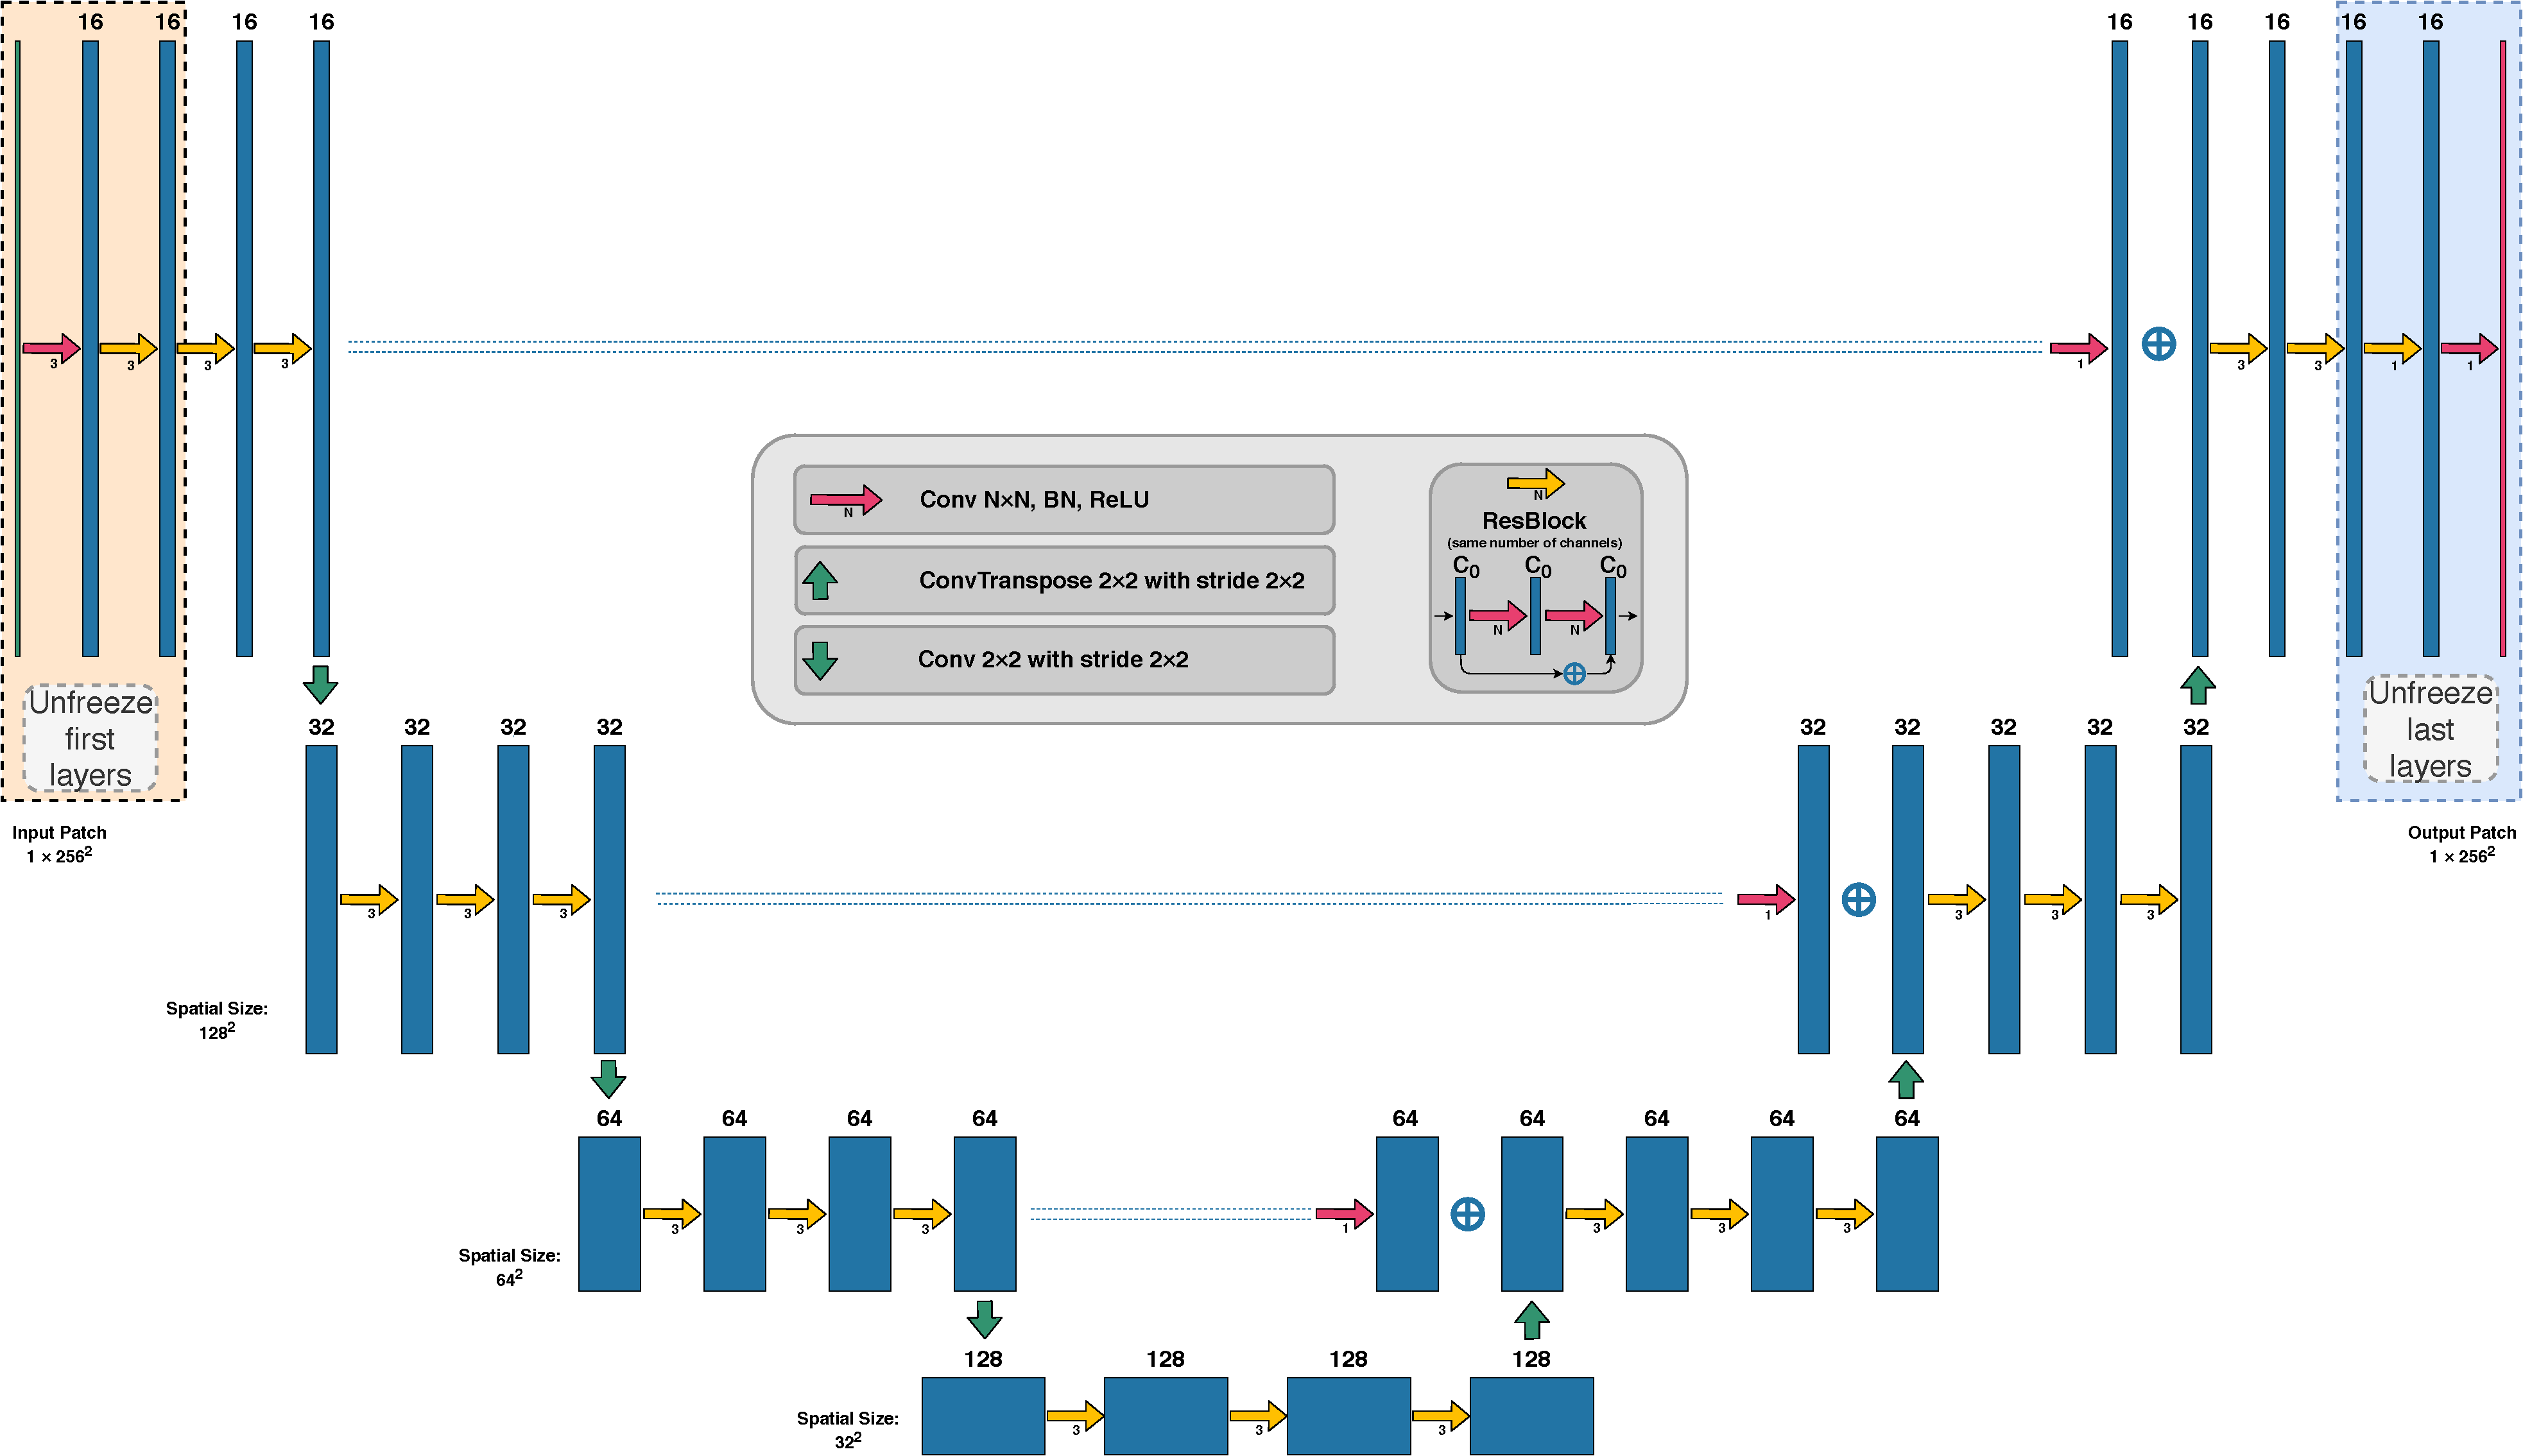
\includegraphics[width=\linewidth]{Dissertation/Figures/2_mri/unet2d_da.pdf}
	\caption{The architecture of 2D U-Net with minor modification we use in our work.} %In the scenarios implying network weights freezing, either the first or last three convolutional layers are available for fine-tuning. These layers contain an equal amount of filters (16) of the same size, which means that in both scenarios an approximately equal number of parameters is fine-tuned.}
	\label{fig:mri:unet2d_da}
\end{figure}
\end{landscape}


\subsection{Adaptive fine-tuning}

Supervised DA in medical image segmentation traditionally relies on explicit decisions regarding which layers of a neural network should be fine-tuned. But there is no clear consensus on whether the initial or final layers should be targeted. Moreover, with the increasing complexity of neural network architectures---often involving skip connections and residual pathways---the challenge extends to identifying the ``first'' layers within these intricate structures. Residual networks, for instance, can behave like ensembles of shallower networks \cite{veit2016residual}, complicating the decision-making process regarding which layers to adapt for optimal domain transfer.
%\cite{bakas2018identifying}

To address these challenges, we propose an extension of the SpotTune framework \cite{guo2019spottune} tailored for supervised DA in medical image segmentation, which we call \textbf{SpotTUnet}. SpotTUnet introduces a dynamic and adaptive approach to layer selection, leveraging a policy network to make real-time decisions on whether to fine-tune or freeze specific layers within a network.

SpotTUnet consists of three main components: two copies of the main segmentation network and a policy network, as illustrated in Figure~\ref{fig:spottune_seg}. The segmentation  U-Net network, which is described in Section~\ref{sec:mri:method:sft}, is initially pretrained on the source domain dataset. Then, this model is duplicated into two versions and supplemented with the policy network:

\begin{enumerate}
	
	\item \textbf{Frozen Network (Blue Blocks):} The first copy retains the pretrained weights and remains fixed during the fine-tuning process. This network serves as a baseline, preserving the knowledge learned from the source domain.
	
	\item \textbf{Fine-Tuned Network (Orange Blocks):} The second copy is subject to fine-tuning on the target domain dataset. This network adapts to the new domain, with its weights initialized with the pretrained ones and being updated based on the target data.
	
	\item \textbf{Policy Network (Red Blocks):} This model is responsible for predicting whether each block in the segmentation network should use the frozen or fine-tuned version. It outputs a pair of logits for each of the $N$ blocks (block represents a residual block in our case). A softmax function is applied to these logits, converting them into probabilities for a binary classification task:
	\begin{itemize}
		\item Class 0: Use the frozen block from the pretrained network.
		\item Class 1: Use the fine-tuned block from the updated network.
	\end{itemize}
	
\end{enumerate}


\begin{landscape}
\begin{figure}[p]
	\centering
	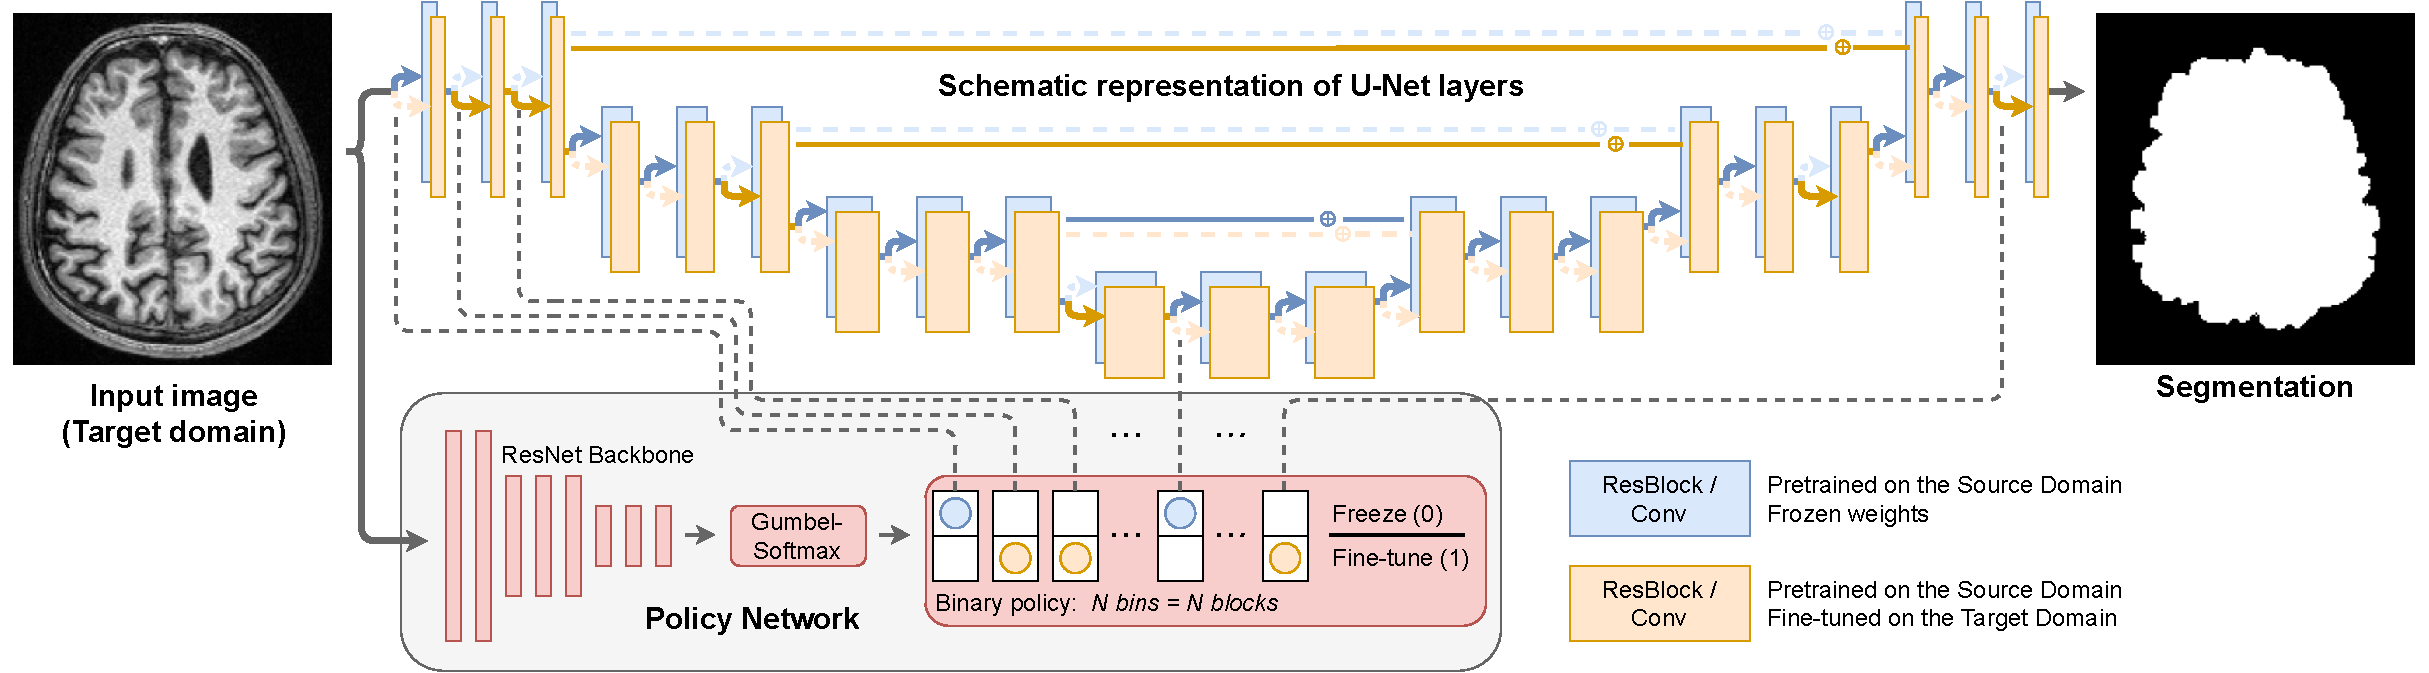
\includegraphics[width=\linewidth]{Dissertation/Figures/2_mri/spottune_seg.pdf}
	\caption{SpotTUnet architecture for the supervised DA in medical image segmentation.}% The U-Net backbone is pretrained on the source domain. This network is frozen (blue blocks) and has a copy (orange blocks) that is fine-tuned on the target domain. The policy network is simultaneously trained on the target domain to output binary decisions for each pair of blocks from the segmentation networks: use the frozen block (blue) vs. use the fine-tuned block (orange).}
	\label{fig:spottune_seg}
\end{figure}
\end{landscape}



The output for the $l$-th block is then computed as:

\begin{equation}
	x_l = I_l ( x ) F_l ( x_{l-1} ) + (1 - I_l ( x )) \tilde{F}_l ( x_{l-1} ),
\end{equation}

\noindent
where $F_l$ and $\tilde{F}_l$ represent the frozen and fine-tuned versions of the $l$-th block, respectively, and $I_l(x)$ is the binary indicator derived from the Policy Network’s prediction.

Policy Network is trained concurrently with the fine-tuning of the segmentation network. During each iteration, Policy Network makes ``soft'' predictions for each block, which we binarize (into $I_l(x)$) to determine whether to use the frozen or fine-tuned block. To ensure gradient flow through the binary decision-making process, we employ the Gumbel-Softmax trick~\cite{jang2017categorical} in the following way.% This approach allows gradients to be propagated through the binary indicator $I_l(x)$, enabling end-to-end training.

The binary indicator $I_l(x) \in \{0, 1\}$ represents a discrete decision, which is inherently non-differentiable. To enable gradient-based optimization, we replace this hard decision with a differentiable approximation based on the Gumbel–Softmax (also known as the Concrete) distribution.

Let the Policy Network produce for each block $l$ a pair of unnormalized logits

\[
\mathbf{z}_l(x) = [z_{l,0}(x),\, z_{l,1}(x)],
\]

\noindent
corresponding to the probabilities of using the frozen ($I_l=0$) or fine-tuned ($I_l=1$) version of the block. The categorical sampling operation

\[
I_l(x) \sim \mathrm{Categorical}(\pi_{l,0}, \pi_{l,1}), \quad
\pi_{l,i} = \frac{\exp(z_{l,i})}{\sum_{j} \exp(z_{l,j})},
\]

\noindent
is replaced by a continuous relaxation:

\begin{equation}
	\tilde{I}_l(x) =
	\frac{
		\exp\!\left((z_{l,1} + g_1)/\tau\right)
	}{
		\exp\!\left((z_{l,0} + g_0)/\tau\right) +
		\exp\!\left((z_{l,1} + g_1)/\tau\right)
	},
	\label{eq:gumbelsoftmax}
\end{equation}

\noindent
where $g_0, g_1$ are independent samples from the $\mathrm{Gumbel}(0,1)$ distribution,

\[ g = -\log(-\log u), \quad u \sim \mathrm{Uniform}(0,1), \]

\noindent
and $\tau > 0$ is a temperature parameter controlling the smoothness of the approximation. In the limit $\tau \to 0$, the expression in~\eqref{eq:gumbelsoftmax} approaches a hard binary decision, while for higher $\tau$ values, it yields a smooth, differentiable interpolation between the two options. %During training, $\tau$ is typically annealed towards zero to gradually enforce discreteness while preserving gradient flow in the early stages of optimization.

In our framework, we define the effective indicator as

\[
I_l(x) =
\begin{cases}
	1, & \tilde{I}_l(x) > 0.5, \\
	0, & \text{otherwise},
\end{cases}
\quad \text{(forward pass)}
\]

\noindent
while in the backward pass, gradients are propagated through the continuous relaxation $\tilde{I}_l(x)$. This approach ensures that the Policy Network receives meaningful gradients even though the decision process is discrete at inference time.
% , often referred to as the \emph{straight-through Gumbel--Softmax estimator},

\textbf{Regularization of the Adaptive Policy.} While the Gumbel–Softmax relaxation enables end-to-end optimization of the discrete adaptation policy, it does not by itself control the complexity of the resulting fine-tuning pattern. Without additional constraints, the Policy Network may assign all blocks to be fine-tuned, which can lead to over-parameterization and overfitting -- a critical issue when the amount of annotated target-domain data is limited.

To address this, we introduce a regularization term that penalizes the number of fine-tuned blocks directly at the policy level. In addition to the standard segmentation loss~($\mathcal{L}_{segm}$), the total loss is defined as


\begin{equation}
	\mathcal{L} \;=\; \mathcal{L}_{segm}
	\;+\;
	\lambda \sum_{l=1}^{N} \big(1 - I_l(x)\big),
	\label{eq:loss_total}
\end{equation}

\noindent
where $\lambda$ is a regularization coefficient controlling the trade-off between segmentation performance and the sparsity of adaptation. This term can be viewed as an $\mathbb{L}_1$ penalty on the Policy Network’s binary outputs $\{I_l(x)\}_{l=1}^N$, directly encouraging the network to activate fewer fine-tuned blocks.

Conceptually, this formulation replaces the global structural constraint used in the original SpotTune method~\cite{guo2019spottune}. In SpotTune, the so-called \emph{Global-$k$} policy enforces that all images share the same subset of $k$ fine-tuned layers, thereby coupling the adaptation decisions across the dataset. In contrast, our approach defines an \emph{instance-wise} policy governed by~\eqref{eq:loss_total}, in which each image $x$ may activate a different combination of fine-tuned and frozen blocks, while the $\mathbb{L}_1$ penalty ensures that the overall number of active (fine-tuned) blocks remains low.

This modification has two main advantages. First, it provides a simpler and more interpretable regularization mechanism, with only one tunable hyperparameter~$\lambda$ instead of the discrete variable~$k$. Second, it better adapts to varying amounts of available target data: for larger datasets, the model can afford to fine-tune more blocks, whereas in low-data regimes, the regularization naturally promotes more frozen configurations, reducing overfitting risk. In practice, the $\mathbb{L}_1$ regularization term serves as an adaptive sparsity prior on the Policy Network outputs, enabling flexible yet controlled domain adaptation behavior across different training conditions.

Below we compare SpotTUnet with the other fine-tuning approaches and extensively analyze domain shift anatomy using obtained Policy Network.


%\paragraph{Policy learning and differentiable relaxation.}
%Policy Network is trained concurrently with the fine-tuning of the segmentation network. During each iteration the Policy Network produces soft logits for each block, which are then mapped to a (relaxed) binary decision that selects between the frozen and fine-tuned versions of the block. To permit gradient flow through this inherently discrete decision we employ the Gumbel--Softmax (Concrete) relaxation [?]. Concretely, let the Policy Network output unnormalized logits
%\[
%\mathbf{z}_l(x) = \bigl(z_{l,0}(x),\, z_{l,1}(x)\bigr),
%\qquad \pi_{l,i} = \frac{\exp(z_{l,i})}{\sum_j \exp(z_{l,j})}.
%\]
%We draw independent Gumbel samples $g_0,g_1 \overset{\mathrm{iid}}{\sim}\mathrm{Gumbel}(0,1)$ (via $g=-\log(-\log u)$, $u\sim\mathcal{U}(0,1)$) and form the continuous relaxation
%\begin{equation}
%	\tilde{I}_l(x) \;=\;
%	\frac{\exp\bigl((z_{l,1}(x) + g_1)/\tau\bigr)}
%	{\exp\bigl((z_{l,0}(x) + g_0)/\tau\bigr) + \exp\bigl((z_{l,1}(x) + g_1)/\tau\bigr)},
%	\label{eq:gumbelsoftmax_relax}
%\end{equation}
%where $\tau>0$ is a temperature parameter. For training we use the straight-through style implementation: in the forward pass the binary indicator is taken as
%\[
%I_l(x) \;=\; \mathbf{1}\{\tilde{I}_l(x) > 0.5\},
%\]
%while in the backward pass gradients are propagated through the continuous quantity $\tilde{I}_l(x)$ (i.e., the backward pass uses $\partial \tilde{I}_l/\partial z$). This practical scheme reduces the train–test mismatch while preserving train-time gradient information. 
%
%The formal justification for replacing the discrete sampler by the Gumbel--Softmax relaxation is twofold. First, for any fixed $\tau>0$ the mapping in \eqref{eq:gumbelsoftmax_relax} is smooth and admits low-variance reparameterized gradients with respect to the logits, enabling standard backpropagation. Second, as the temperature is annealed, the Gumbel--Softmax distribution concentrates on the simplex vertices and its samples converge to one-hot samples from the categorical distribution; thus the relaxation smoothly interpolates between a fully continuous gate and the desired discrete gate, and optimizing the relaxed objective with an annealing schedule approximates optimizing the original discrete objective in the low-temperature limit. For details on the density, reparameterization and the limiting behaviour see \cite{Jang2017,Maddison2017}.
%
%Consequently, our full training objective remains
%\[
%\mathcal{L} \;=\; \mathcal{L}_{segm} \;+\; \lambda \sum_{l=1}^N \big(1 - I_l(x)\big),
%\]
%with $I_l(x)$ implemented as above (forward hard threshold, backward relaxed gradient). In practice we anneal $\tau$ during training and tune $\lambda$ to trade off segmentation accuracy and the number of fine-tuned blocks.



\section{Experiments}


\subsection{Data}

We conducted all experiments using the publicly available CC359 dataset \cite{souza2018open}, which consists of 359 head MRI scans. These scans were acquired using scanners from three different vendors: Siemens, Philips, and General Electric. Each vendor's scanners operate at two different magnetic field strengths, 1.5 T and 3 T, resulting in a total of six distinct domains within the dataset. The data distribution is balanced across these domains, with the exception of the Philips 1.5 T domain, which contains only 59 subjects. Using this dataset, we address the brain segmentation task from brain MRI scans.

For preprocessing, we applied two straightforward steps. First, all scans were resampled to a uniform voxel resolution of $1 \times 1 \times 1$ mm using linear interpolation. Second, the voxel intensities of the resampled images were normalized to a range between 0 and 1 before being fed into the network. No additional preprocessing was applied to the data.


\subsection{Experimental setup}
%\label{sec:mri:exp:setup}

We conducted three primary groups of experiments to evaluate our approach. Throughout this section, the term \textit{scan} refers to a complete 3D MRI study, while \textit{slice} denotes a 2D section of a scan.

\textbf{Baseline and Oracle.} To assess the suitability of the CC359 dataset for DA experiments, we first established a \textbf{Baseline} for cross-domain model transferability. We trained six separate models, each on a distinct domain, and then tested each model across the remaining target domains. This Baseline provides a foundational comparison for subsequent experiments.

The model's performance within the source domain was evaluated using 3-fold cross-validation, referred to as the \textbf{Oracle} score. This score represents the ``ideal'' reference score for all transfer methods, though it is theoretically possible for some methods to surpass Oracle in certain cases.

In the subsequent transfer experiments, models trained on the entire source domain were transferred to target domains. We evaluated the effectiveness of these methods by calculating the fraction of the performance gap between the oracle and the baseline that each method was able to close. This metric provides a clear and interpretable measure of methods performance.


\textbf{Predefined fine-tuning.} The first focus of our study is on three supervised domain adaptation strategies: fine-tuning the entire model (all layers), fine-tuning only the initial layers, and fine-tuning only the final layers.

Our goal was to assess the performance of these strategies under varying conditions of data availability, particularly in scenarios with an extreme scarcity of target domain data. Preliminary experiments indicated that segmentation quality begins to decline when fewer than five scans are available, which aligns with findings from previous studies \cite{valverde2019one}, where segmentation performance decreased as the number of voxels in the ground truth mask was reduced. By using a 2D network, we were able to work with a subset of slices from a single scan instead of reducing the ground truth mask, which was not feasible for our task.

We varied the amount of available data, starting with 3 and 1 target MRI scans. Leveraging our 2D architecture, we further subsampled slices from a single scan at fractions of $1/2$, $1/3$, $1/6$, $1/12$, $1/24$, and $1/36$. In these scenarios, slices were evenly sampled with a consistent step; for example, in the $1/3$ scenario, slices 0, 3, 6, and so forth were selected. The total numbers of slices available for fine-tuning are 800, 270, 135, 90, 45, 24, 12, 8, respectively.

We repeat these experiments for each of the 30 source-target pairs in the CC359 dataset.


\textbf{Adaptive fine-tuning.} Again, the six domains in the dataset yielded $30$ source-target pairs, leading to $30$ supervised DA experiments. Since we needed to select SpotTUnet hyperparameters, we reserved one source domain (Siemens, $1.5$ T) and its corresponding 5 source-target pairs for SpotTUnet validation, using the remaining 25 pairs to test designed DA approaches.

For the $5$ validation pairs, we first tuned the temperature parameter of Gumbel-Softmax ($\tau$) through grid-search, exploring values $\tau \in \{ .01, .1 , .5, 1, 2, 5 \}$. The number of annotated slices from the target domain was fixed at 270 (equivalent to one scan). Next, we optimized the $\lambda$ parameter for each level of target data availability via grid-search over $\lambda \in \{0, 1, 3 , 5, 7, 10, 12, 15, 20 \} \times 10^{-3}$. The latter validation experiment and all testing experiments addressed the same scenarios for target data scarcity, with $8$, $12$, $24$, $45$, $90$, $270$, and $800$ slices available for fine-tuning. The optimal $\lambda$ value was fixed for each data scarcity scenario and applied to SpotTUnet during testing on the remaining $25$ pairs.

%\textbf{Discussion of the additional setups.} Despite the authors of \cite{isensee2018no} suggest focusing on the pipeline rather than the peculiarities of an architecture, we support our claim with the same line of experiments with vanilla U-Net architecture \cite{ronneberger2015u}. Moreover, extremely limited amounts of data available raise the question of augmentation, thus we repeat all the experiments for both architectures, introducing simple augmentation techniques: rotations and symmetric flips. We place all the results for vanilla U-Net and the results for the original net trained with augmentation in Supplementary Materials while discussing them in Sec. \ref{sec:results}.

%In our preliminary experiments we also tried other supervised DA setups. First, instead of fine-tuning, we trained the model from scratch on joint data from the source and the target domains. Secondly, we trained the model from scratch on data from the target domain only. We do not include aforementioned strategies in the further analysis for they yield extremely poor results.


\subsection{Evaluation metrics}

The quality in medical image segmentation problems is typically assessed using the Dice Score \cite{bakas2018identifying}, which is defined as

\begin{equation}
	\label{eq:dice_score}
	\text{Dice Score} = \frac{2 \cdot |A \cap B|}{|A| + |B|},
\end{equation}

\noindent
where $A$ and $B$ represent the predicted and ground truth masks (sets of voxels), respectively. This metric measures the voxel-wise overlap between the two masks, providing a volumetric assessment of segmentation quality. However, in brain segmentation, the accuracy of delineating the brain's edges is a crucial indicator of model performance. Given that edge regions constitute a relatively small portion of the brain's overall volume, the Dice Score may lack sensitivity in capturing the quality of boundary delineation.

To address this limitation, we also employ the Surface Dice Score~\cite{nikolov2021clinically}, which specifically evaluates how closely the predicted and ground truth surfaces align. Although the Surface Dice metric shares the same mathematical formula as the Dice Score (\ref{eq:dice_score}), in this context, $A$ and $B$ correspond to the surfaces of the segmented regions rather than entire volumes. The key difference lies in the concept of \textit{tolerance}, which specifies the maximum allowable distance between corresponding surface voxels for them to be considered as matching. For our experiments, we report results using a tolerance of 1 mm, as we find this threshold to be sufficiently sensitive to variations in the predictions across different methods.

To further evaluate the effectiveness of each domain adaptation (DA) method, we calculate the proportion of the gap between the Oracle and Baseline scores that the method closes. This proportion, denoted as $D_R$, is defined as follows:

Finally, to assess each DA method for a particular source-target pair we calculate the share of the gap between Oracle and Baseline this method closes. We denote this share $D_R$ and define it the following way:

\begin{equation}
	D_R = \dfrac{D - D_B}{D_O - D_B} = \dfrac{\Delta(transferring)}{\Delta(oracle)},
\end{equation}

\noindent
where $D_O$ represents the Oracle Surface Dice Score on the target domain, $D_B$ is the Baseline score on the target domain, and $D$ is the score of the adaptation method under consideration. This metric provides a clear and interpretable measure of how effectively each DA method improves upon the Baseline, relative to the Oracle.


\subsection{Architecture and Training}

In this study, we opted for a 2D U-Net architecture \cite{ronneberger2015u} rather than a 3D CNN, as it allows us to explore the performance of various approaches on a very limited amount of labeled data from the target domain--specifically, a subset of slices from a single scan. All necessary modifications to the original U-Net architecture are detailed in Section~\ref{sec:mri:method:sft}. Additionally, we conducted baseline experiments using a 3D U-Net \cite{cciccek20163d}, observing a similar decline in segmentation quality. We also repeated the experimental pipeline with the vanilla U-Net to confirm the consistency of our results.

On the source domain, the model was trained for 100 epochs, beginning with a learning rate of $10^{-2}$, which was reduced to $10^{-3}$ at epoch 80. For domain transfer, we fine-tuned the model for 60 epochs, starting with a learning rate of $10^{-3}$ and reducing it to $10^{-4}$ at epoch 45. Each epoch comprised 100 iterations of stochastic gradient descent with Nesterov momentum (set to $0.9$). During each iteration, we randomly sampled a slice, cropped it to a size of $256 \times 256$, and formed a mini-batch of $32$ such samples, which were then passed through the network. Binary Cross-Entropy was used as the segmentation loss function ($\mathcal{L}_{segm}$).

Training for 100 epochs required approximately 4 hours on a 16GB NVIDIA Tesla V100 GPU on Zhores supercomputer \cite{zacharov2019zhores}.


\section{Results}


\subsection{Baseline and Oracle}

Table~\ref{tab:mri_baseline} illustrates the domain shift problem in our experiments. When evaluating the 2D U-Net model on the source domain using cross-validation, we observe high Surface Dice values, representing the \textit{Oracle} performance (diagonal elements). However, when the model is transferred to a different domain without fine-tuning (non-diagonal elements, referred to as the \textit{Baseline}), there is a significant drop in segmentation quality. The best scores are highlighted in bold, while the lowest are indicated in italics to emphasize the impact of domain shift.




\begin{table}[h!]
	\centering
	\caption{\textbf{Cross-domain model performance without fine-tuning.} Column headers represent the source domains on which the model was trained, while row headers correspond to the target domains on which the model was tested. ``Sm,'' ``GE,'' and ``Ph'' refer to vendors Siemens, GE, and Philips, respectively. Results are reported as Surface Dice Scores, with corresponding standard deviations in parentheses.}
	\label{tab:mri_baseline}
	
	\begin{tabular}{lcccccc}
		\toprule
		& Sm, 1.5T & Sm, 3T & GE, 1.5T & GE, 3T & Ph, 1.5T & Ph, 3T \\
		\midrule
		Sm, 1.5T & \textbf{.85 (.12)} & .51 (.15) & .72 (.08) & .56 (.13) & .71 (.10) & .71 (.07) \\
		
		Sm, 3T   & .72 (.08) & \textbf{.88 (.03)} & .70 (.07) & .67 (.10) & .63 (.10) & .66 (.06) \\
		
		GE, 1.5T & .39 (.14) & \textit{.09 (.05)} & \textbf{.87 (.05)} & \textit{.30 (.10)} & .55 (.19) & .48 (.08) \\
		
		GE, 3T   & .80 (.05) & .63 (.13) & .66 (.10) & \textbf{.89 (.03)} & .67 (.10) & .67 (.06) \\
		
		Ph, 1.5T & .63 (.08) & \textit{.25 (.07)} & \textbf{.87 (.03)} & .43 (.06) & \textbf{.89 (.03)} & .46 (.08) \\
		
		Ph, 3T   & .54 (.13) & .34 (.13) & .70 (.11) & .37 (.10) & .47 (.14) &  \textbf{.86 (.04)} \\
		\bottomrule
	\end{tabular}
\end{table}



\subsection{Predefined fine-tuning}

In this section, we compare three approaches to supervised DA: fine-tuning the entire model (\textit{all layers}), fine-tuning only the \textit{initial (first) layers}, and fine-tuning only the \textit{final (last) layers}.

We analyze how the relative improvement score $D_R$ depends on the amount of training data available from the target domain. Figure~\ref{fig:gap} shows the average scores across 30 possible source-target domain pairs. The figure also presents the distribution densities of these scores for each strategy.

\begin{figure}[h!]
	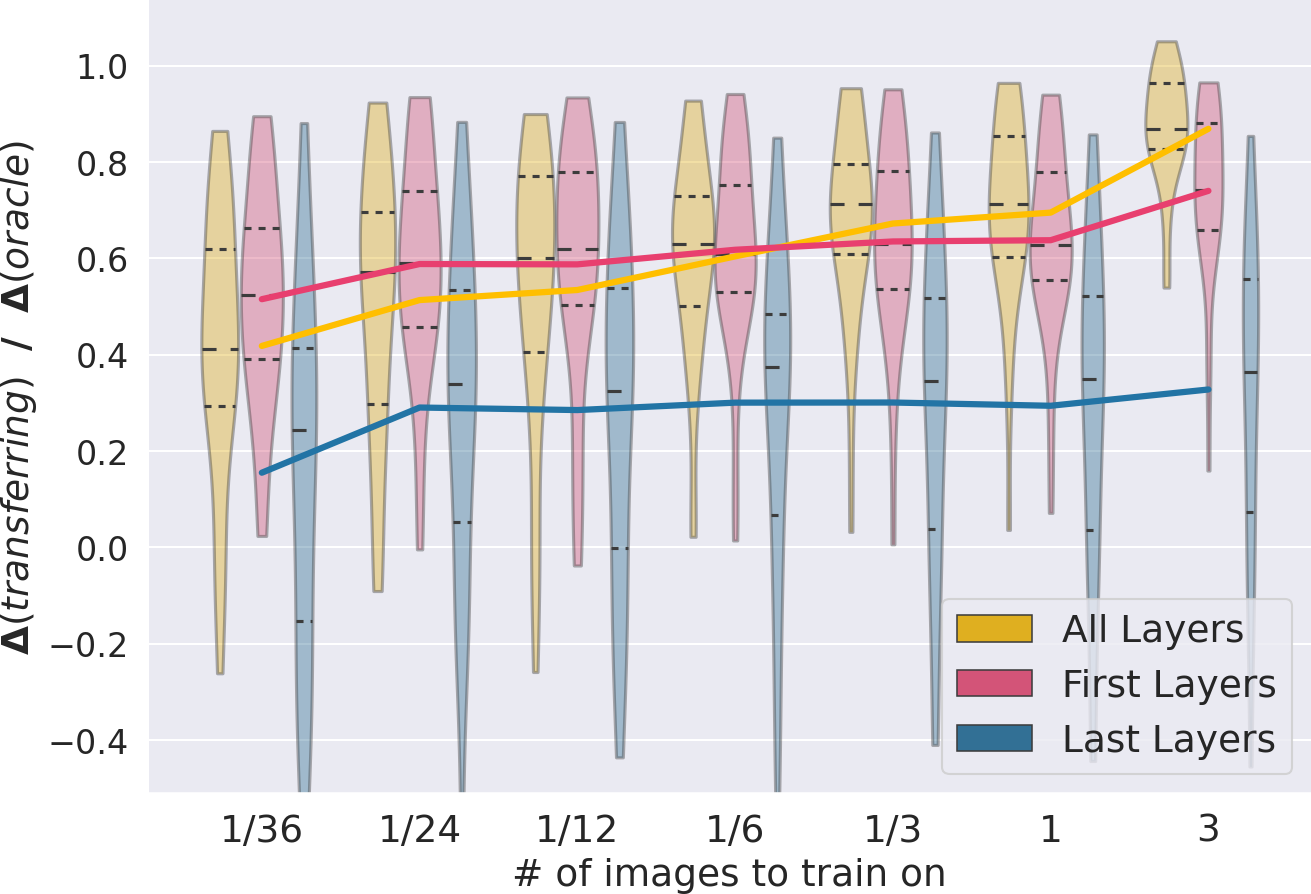
\includegraphics[width=\linewidth]{Dissertation/Figures/2_mri/gap.png}
	\caption{Dependence of the relative Surface Dice improvement (y-axis, $D_R$) on the availability of target domain data (x-axis) for the three transfer strategies. The lines represent average scores, while the density distributions reflect scores across 30 source-target pairs for each strategy.}
	\label{fig:gap}
\end{figure}

In Figure~\ref{fig:winners}, we report the number of source-target pairs where a given method outperforms the others (summing to 30 across all methods for each setup). Contrary to common assumptions, our results show that fine-tuning the initial layers significantly outperforms fine-tuning the final layers in our task. This finding suggests that low-level features, which correspond to the image's intensity profile, can be more effectively re-learned than high-level features, which are associated with different brain structures and distinct shapes.

\begin{figure}[h]
	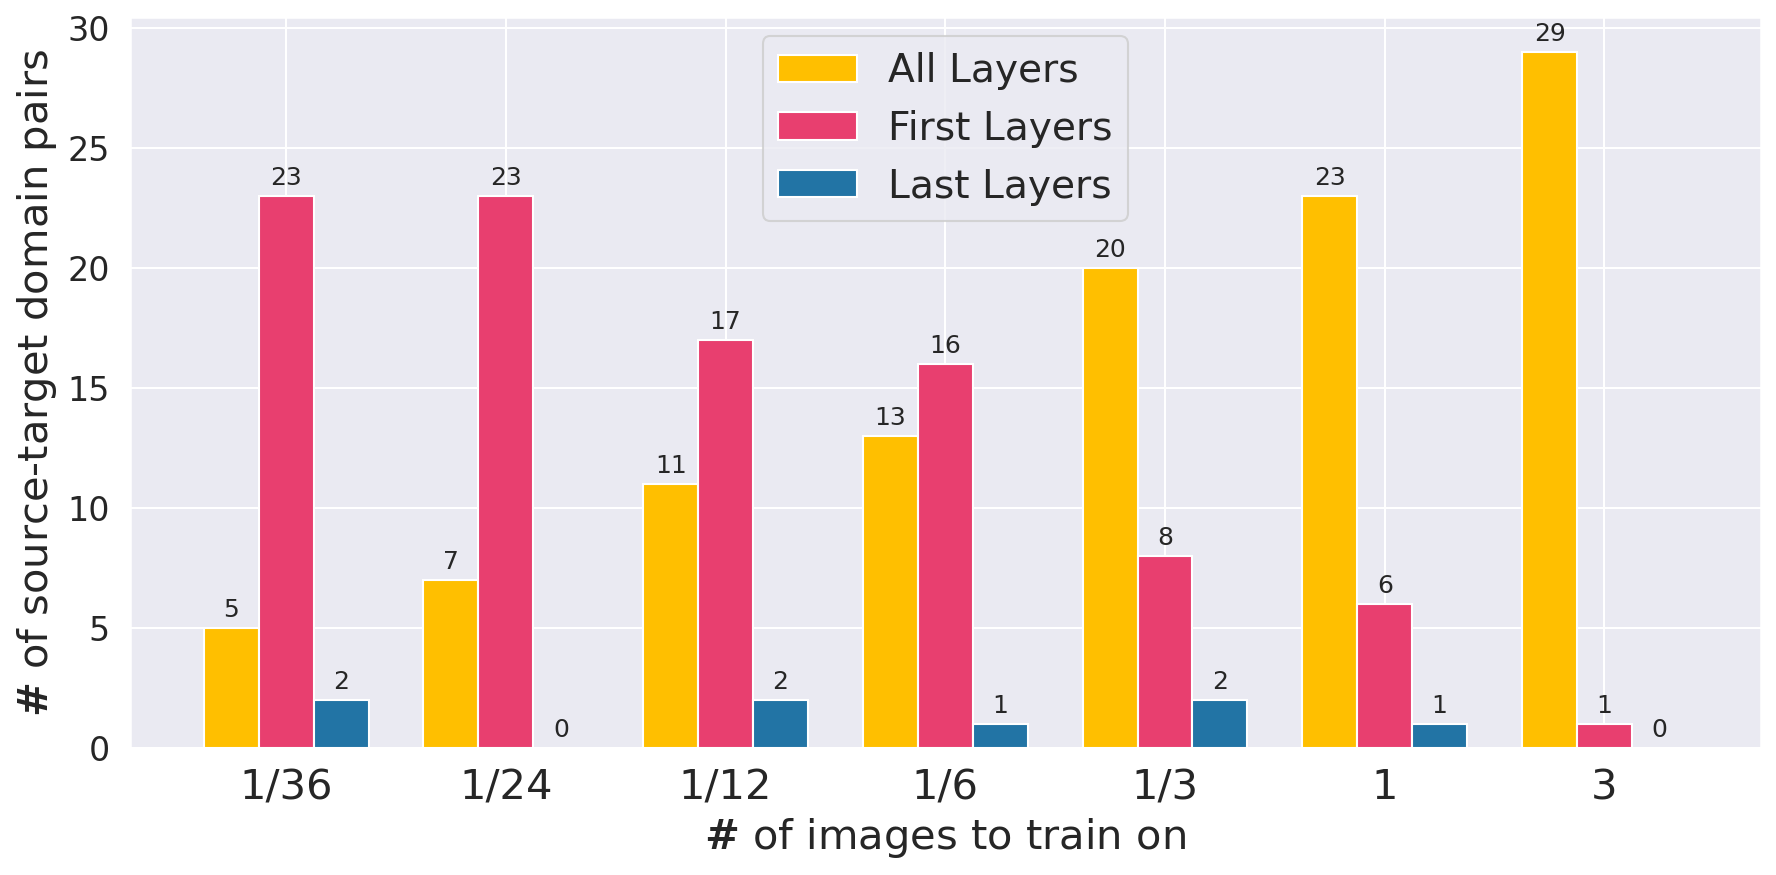
\includegraphics[width=\linewidth]{Dissertation/Figures/2_mri/winners_1.png}
	\caption{Effectiveness of each domain adaptation strategy based on target domain data availability. Each bar represents the number of source-target pairs for which a given method is the most effective.}
	\label{fig:winners}
\end{figure}


Moreover, under conditions of extreme data scarcity, fine-tuning the initial layers proves to be more advantageous than fine-tuning the entire model. This makes the former approach particularly valuable in practical scenarios where annotated target domain data is limited.


The observed trends remain consistent even when substituting U-Net with residual blocks with the vanilla U-Net or adding augmentation. %\todo{Results for these setups are available in the Supplementary materials.}% TODO: add supplementary results to Appendix


\subsection{Adaptive fine-tuning}

%We begin by tuning and selecting the hyperparameters for SpotTUnet through validation.

The temperature of the Gumbel-Softmax is set to $\tau = 0.1$, while the optimal regularization parameter $\lambda$ is determined separately for each data scarcity scenario; see Figure~\ref{fig:lambda}. It is important to note that the stability of Gumbel-Softmax training is highly sensitive to the choice of $\tau$, so we recommend validating different values of $\tau$ early in the deployment of SpotTune-like architectures.

\begin{figure}[h]
	\centering
	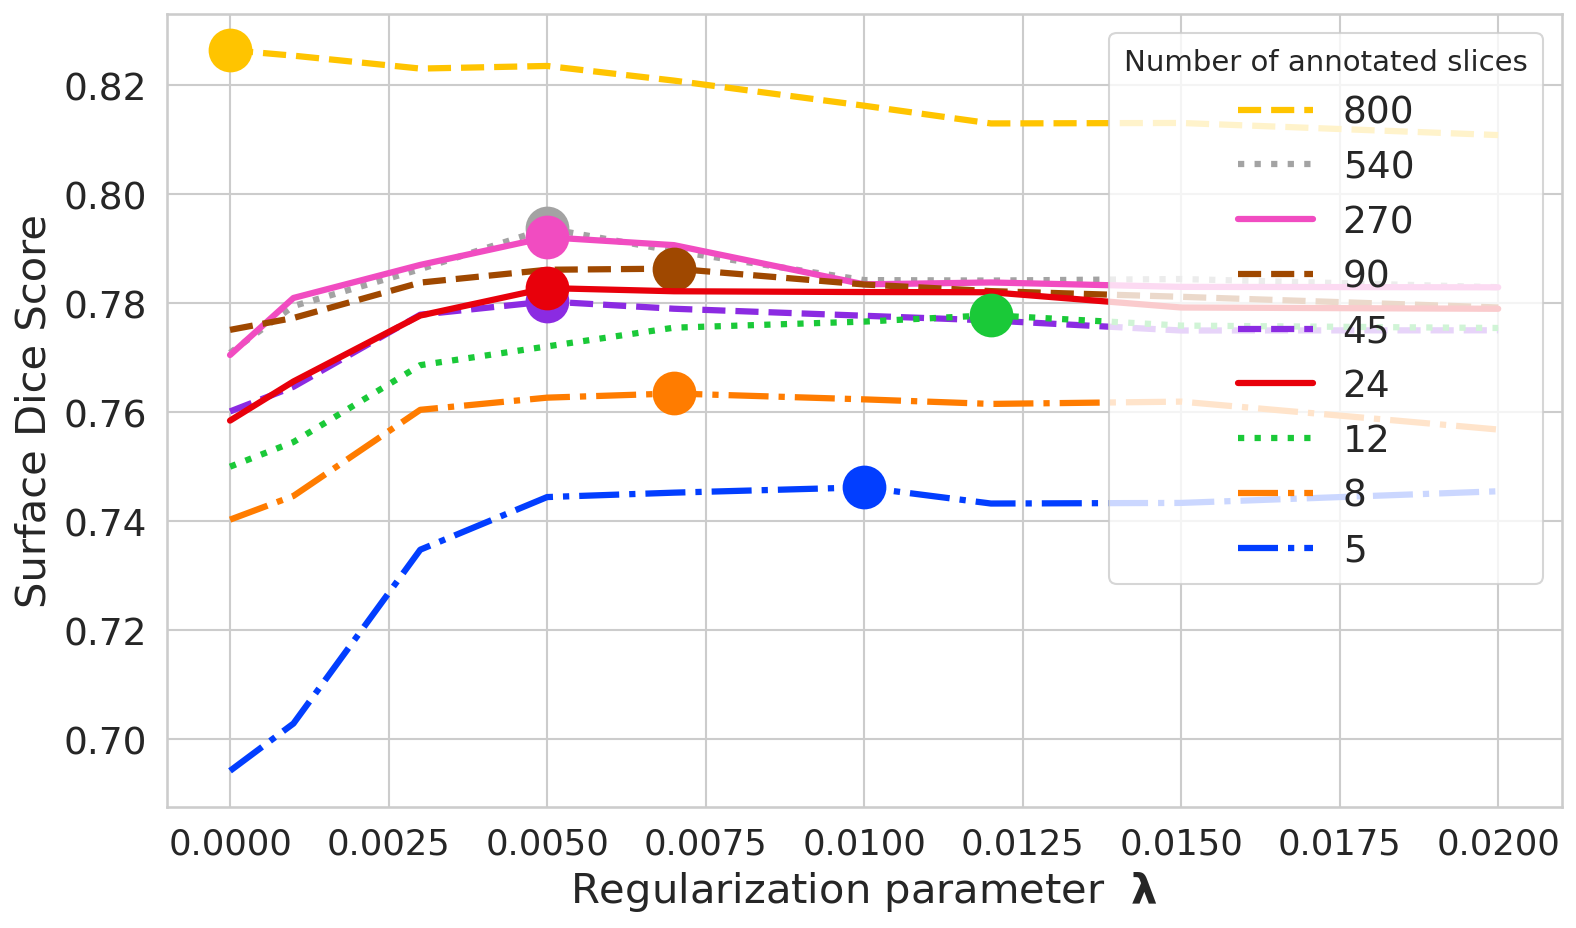
\includegraphics[width=\textwidth]{Dissertation/Figures/2_mri/k_reg.png}
	\caption{\textbf{Validation performance of SpotTUnet as a function of the regularization parameter $\lambda$.} Each point represents the average Surface Dice Score across 5 validation experiments. Each line corresponds to a different amount of annotated data from the target domain, with bold points indicating the optimal $\lambda$ values based on Surface Dice Score.}
	\label{fig:lambda}
\end{figure}

We found that a positive regularization term significantly benefits most data scarcity setups: the surface Dice Score with the optimal $\lambda$ is significantly higher ($p < 10^{-3}$, one-sided Wilcoxon signed-rank test) than that of the corresponding model without regularization. The only exception is the case with 800 available target slices (approximately three 3D images), where the optimal $\lambda$ is close to zero, and increasing $\lambda$ leads to a drop in quality (Figure~\ref{fig:lambda}). This suggests that while SpotTUnet can learn the optimal policy without regularization when target data is abundant, regularization significantly enhances DA performance when target data is scarce.

Next, we compare SpotTUnet with the previously developed approaches: \textit{Fine-Tune All Layers} and \textit{Fine-Tune First Layers}. Strategy of \textit{fine-tuning the last layers} is excluded from comparison due to previously shown poor performance. Figure~\ref{fig:sdcs} shows the distributions of the Surface Dice Scores (violin plots) alongside their average values (lines). Our results demonstrate that SpotTune performs on par with the best of the other methods, regardless of the severity of target data scarcity.

\begin{figure}[h]
	\centering
	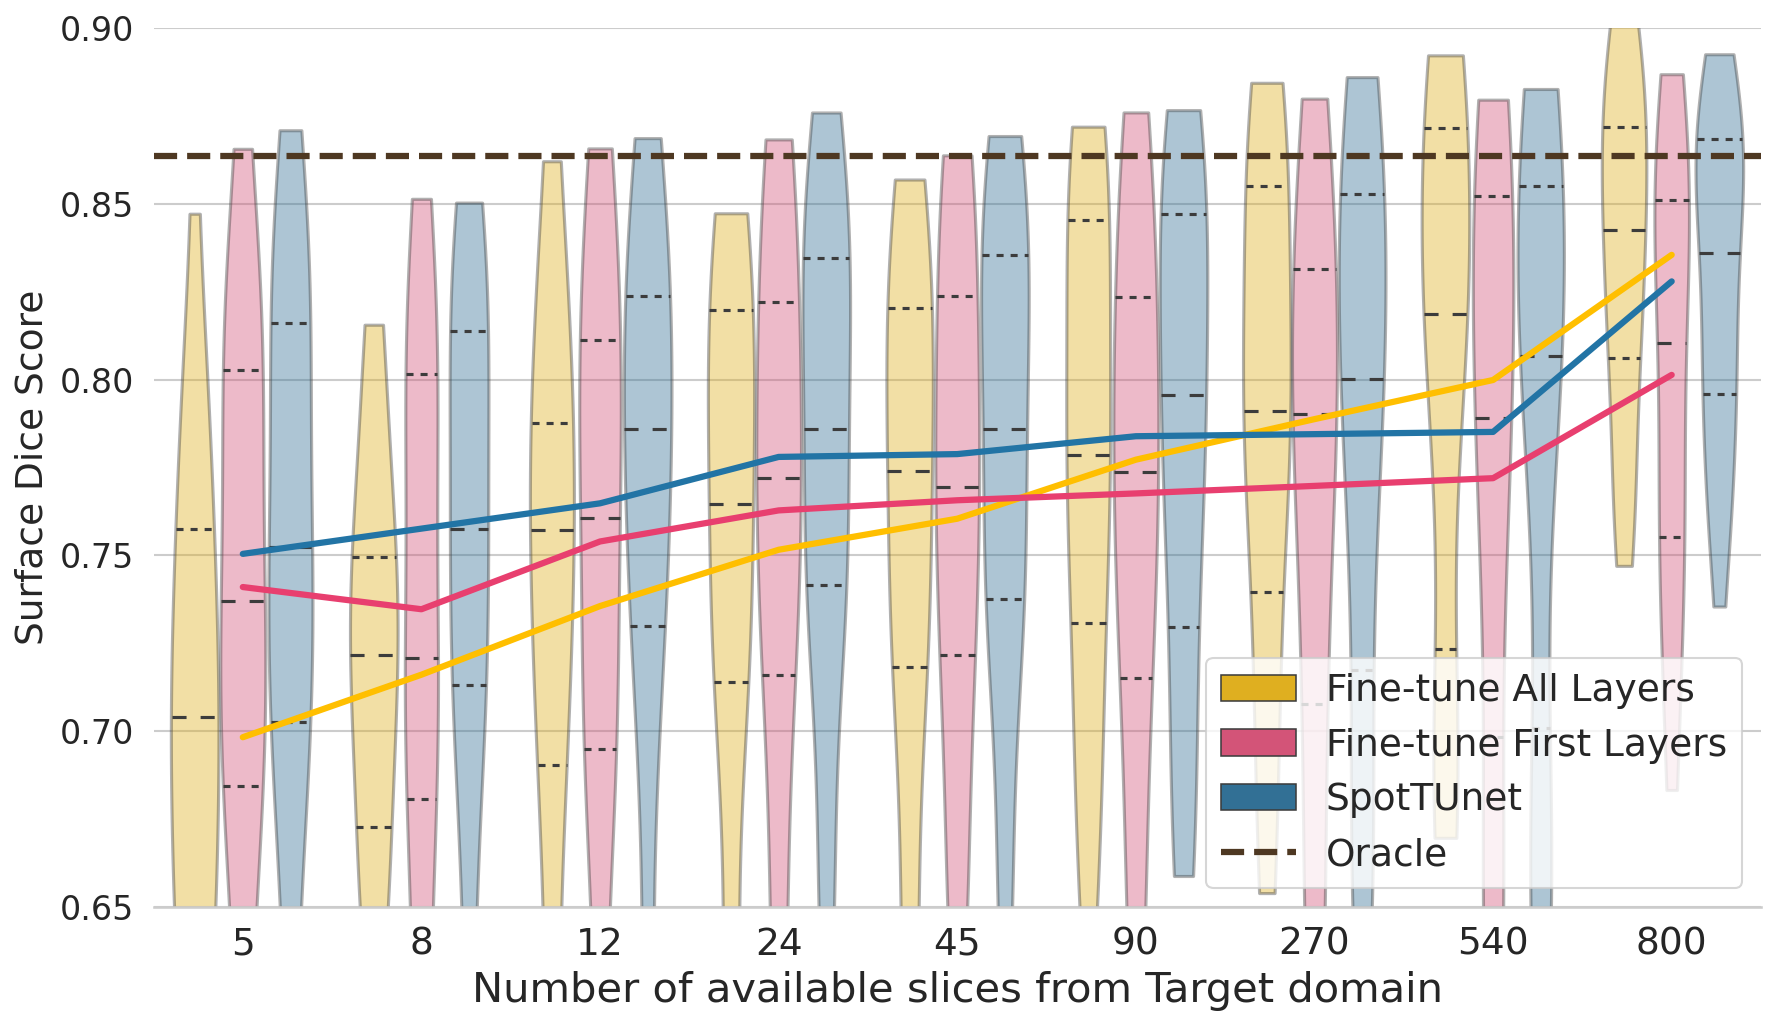
\includegraphics[width=\textwidth]{Dissertation/Figures/2_mri/sdsc.png}
	\caption{Performance of methods as a function of target domain data availability.}
	\label{fig:sdcs}
\end{figure}

Finally, we examine the policy learned by SpotTUnet on the test data by calculating the frequency with which each layer is fine-tuned versus kept pretrained and frozen. The layer-wise visualization is shown in Figure~\ref{fig:layerswise_template}. We find that blocks in the encoder part of the U-Net are more frequently fine-tuned, particularly when annotated data is scarce. However, these are not necessarily the first layers (e.g., those preserving the original resolution), which contrasts with our previous findings, reported in \cite{shirokikh2020first}. We hypothesize that the SpotTUnet policy highlights layers that should be fine-tuned for optimal performance. Consequently, feature maps preceding these frequently fine-tuned layers might be more susceptible to domain shifts. It may be worthwhile to explore whether unsupervised DA approaches \cite{kamnitsas2017unsupervised, zhao2021robust} could benefit from passing these domain-shift-prone feature maps to adversarial networks---a hypothesis we leave for future research.

\begin{landscape}
\begin{figure}[p]
	\centering
	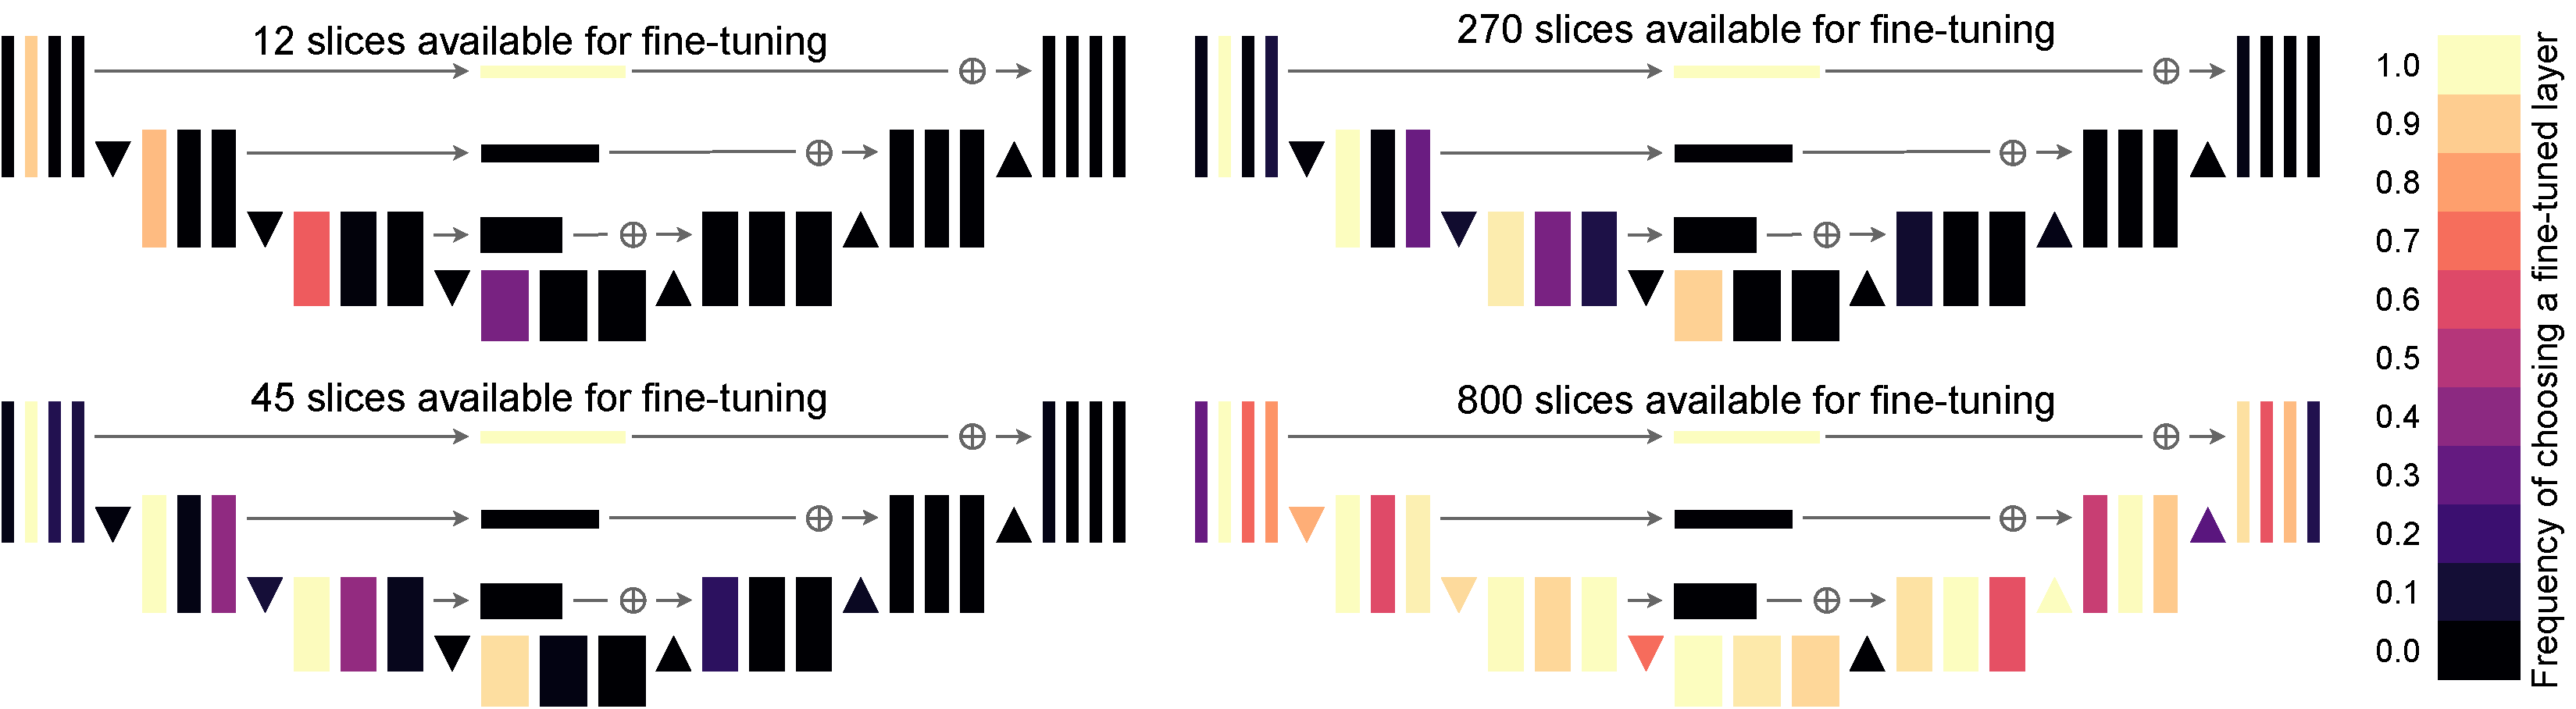
\includegraphics[width=\linewidth]{Dissertation/Figures/2_mri/layerwise_template.pdf}
	\caption{Visualization of SpotTUnet's learned policy for different amounts of available target slices: 12 (upper-left), 45 (bottom-left), 270 (upper-right), and 800 (bottom-right). Colored blocks correspond to residual blocks, with triangular blocks indicating convolutions that perform $\times 2$ up- or down-sampling.}
	\label{fig:layerswise_template}
\end{figure}
\end{landscape}

The differences between the policies observed here and those reported in the original SpotTune paper \cite{guo2019spottune} (where mostly final layers were fine-tuned) can be attributed to the fundamental differences between Transfer Learning (TL) and DA. In TL, the data often varies significantly in nature, so fine-tuning the later layers is necessary. In DA, however, the datasets are semantically similar (e.g., brain MRI scans), meaning that domain shifts are primarily low-level, requiring fine-tuning of the earlier layers.


\section{Summary}

The study in this chapter highlights a significant drop in segmentation quality when naively transferring models between the domains of the CC359 dataset. We hypothesize that the low-level feature maps in this dataset are more susceptible to domain shifts than those from deeper layers, making the initial layers a primary source of performance degradation. Our findings support this hypothesis, demonstrating that fine-tuning the initial layers yields better results than fine-tuning the final layers. Moreover, in scenarios with limited annotated data in the target domain, fine-tuning the initial layers proves to be more effective than fine-tuning the entire network.

We also introduce a new approach for supervised domain adaptation in medical image segmentation, called SpotTUnet. Our experiments show that SpotTUnet maintains the quality of previous methods while eliminating the need to switch between different approaches based on the availability of target data. Additionally, SpotTUnet autonomously learns which layers to fine-tune for optimal performance in the target domain, offering a valuable policy that identifies the network layers most affected by domain shifts. We believe this policy could guide the development of more robust unsupervised domain adaptation methods by specifically targeting the initial or SpotTUnet-identified layers.



	

%\chapter{Domain shift in CT images}
\chapter{Mitigating Domain Shift from CT Reconstruction Kernels}
\label{chap:ct}

%Domain shift is one of the most salient challenges in medical computer vision. Due to immense variability in scanners’ parameters and imaging protocols, even images obtained from the same person and the same scanner could differ significantly.
In this chapter, we consider variability in computed tomography (CT) images caused by different convolution kernels used in the reconstruction process, the critical domain shift factor in CT. The choice of convolution kernel affects pixel granularity, image smoothness, and noise levels, resulting in images that, while anatomically identical, differ in style.

We analyze several datasets of paired CT images where smooth and sharp images were reconstructed from the same sinograms using different kernels. Despite identical anatomy, the consistency between predictions on these paired images is surprisingly low, with an average Dice score of just $0.46$. Furthermore, we observe a significant decline in COVID-19 segmentation accuracy when models are trained and tested on different reconstruction kernels.

To address this domain shift, we propose two methods. The first is Filtered Back-Projection Augmentation (FBPAug), a novel knowledge-driven augmentation technique designed to simulate domain shifts associated with varying reconstruction kernels. \text{FBPAug} improves prediction consistency from a Dice score of $0.46$ to $0.76$, surpassing other augmentation methods. The second method, F-Consistency, is an unsupervised domain adaptation (DA) approach that leverages paired, unlabeled CT images reconstructed with different kernels. This method enforces similarity in the network’s hidden representations by minimizing the mean squared error (MSE) between feature maps of paired images. Given sufficient paired data, F-Consistency further enhances prediction consistency to a Dice score of $0.80$, outperforming FBPAug, other unsupervised DA methods, and demonstrating superior generalization to unseen kernels.

The results presented in this chapter are based on the author’s publications~\cite{saparov2021zero,shimovolos2022adaptation}.


\section{Background}

Computed tomography (CT) is a widely used method for medical imaging. CT images are reconstructed from the raw acquisition data, represented in the form of a sinogram. Sinograms are two-dimensional profiles of tissue attenuation as a function of the scanner's gantry angle. Here, one of the most common reconstruction algorithms is Filtered Back Projection (FBP) \cite{schofield2020image}. This algorithm has an important free parameter called \textit{convolution kernel}. The choice of a convolution kernel defines a trade-off between image smoothness and noise level \cite{schaller2003spatial}. Reconstruction with a high-resolution kernel yields \textit{sharp} pixels and a high noise level. In contrast, usage of a lower-resolution kernel results in \textit{smooth} pixels and a low noise level. Depending on the clinical purpose, radiologists use different kernels for image reconstruction.

Modern deep neural networks (DNN) are successfully used to automate computing clinically relevant anatomical characteristics and assist with disease diagnosis. However, DNNs are sensitive to changes in data distribution which are known as \textit{domain shift}. Domain shift typically harms models' performance even for simple medical images such as chest X-rays \cite{zech2018variable}. In CT images, factors contributing to domain shift include slice thickness and inter-slice interval, different radiation dose, and reconstruction algorithms, e.g., FBP parameters \cite{kloenne2020domain}. The latter problem is a subject of our interest.
%One could perceptually compare the same image reconstructed with two different kernels in Figure~\ref{fig:consistency_preds}, e.g., B1 and B2.

Recently, several studies have reported a drop in the performance of convolutional neural networks (CNN), trained on \textit{sharp} images while being tested on \textit{smooth} images, e.g., in lung cancer \cite{choe2019deep} and emphysema segmentation \cite{lee2019ct}. The authors of \cite{sandfort2019data} proposed using generative adversarial networks (GAN) to generate realistic CT images imitating arbitrary convolution kernels. A more straightforward approach, simultaneously proposed in \cite{missert2019simulation}, \cite{choe2019deep}, and \cite{lee2019ct}, suggests using a CNN to convert images reconstructed with one kernel to images reconstructed with another. Later, such image-to-image networks can be used either as an augmentation during training or as a preprocessing step during inference.

In this chapter, we show that the domain shift induced by the difference in reconstruction kernels also decreases the quality of the COVID-19 segmentation algorithms. To do so, we construct two domains from the publicly available data: the \textit{source} domain with the \textit{smooth} reconstruction kernels and \textit{target} domain with the \textit{sharp} reconstruction kernels. We train the segmentation model on the source domain and test it on the target domain and validate the most relevant DA methods. In our comparison, we include all related augmentation methods, unsupervised adversarial learning \cite{ganin2015unsupervised}, and two proposed methods \cite{saparov2021zero,shimovolos2022adaptation}.
 
The first proposed method is FBP Augmentation (FBPAug), a novel augmentation method based on the FBP reconstruction algorithm. This augmentation mimics processing steps used in proprietary manufacturer's reconstruction software. We initially apply Radon transformation to all training CT images to obtain their sinograms. Then, we reconstruct images using FBP but with different randomly selected convolution kernels. To show the effectiveness of our method, we compare segmentation masks obtained on a set of paired images, reconstructed from the same sinograms with different convolutional kernels.%These paired images are perfectly aligned; the only difference is their style, smooth or sharp.

We note that the large pools of unlabeled chest CT image pairs which differ only in reconstruction kernels within every pair are publicly available, e.g., \cite{morozov2021simplified}. The intuition here is that the adaptation methods should outperform the augmentation one when a broader range of real-world data is available. Specifically, in such conditions, we propose the second method which enforces the cross-domain feature maps consistency between paired images; we call our method F-Consistency. F-Consistency minimizes the mean squared error (MSE) between the network’s hidden representations (feature maps) of paired images. We expect that explicitly enforcing consistency on the paired images should outperform the adversarial learning that emulates similar behavior minimizing the adversarial loss.

%Our work highlights a domain shift problem in the COVID-19 segmentation task and suggests an efficient solution to this problem. These are our three main contributions:
%% We summarize our three main contributions as follows:
%
%\begin{itemize}
%	
%	\item Firstly, we demonstrate that the difference in CT reconstruction kernels affects the segmentation quality of COVID-19 lesions. The model without adaptation achieves only a $0.56$ Dice Score on the unseen domain, while the best adaptation methods scores $0.64$. In terms of similarity between predictions on the paired images, the baseline Dice Score is $0.46$, which is almost two times lower than the $0.80$ achieved by our method.
%	
%	\item Secondly, we propose FPBAug, a knowledge-driven and efficient approach to augment CT images in sinogram space, emulating reconstruction with different kernels. We show that our method outperforms other augmentation approaches. Moreover, neither specific preparation of source domain data nor target domain data is required, so our publicly released \href{https://github.com/STNLd2/FBPAug}{FBPAug} can be used as a plug-and-play module for zero-shot domain adaptation in CT-based tasks.
%	
%	\item Thirdly, we propose the flexible adaptation approach that outperforms the other considered methods when provided with enough unlabeled data. We also show that our method better generalizes to unseen CT reconstruction kernels and it is less sensitive to the absence of the semantic content (COVID-19 lesions) than the other methods trained on unlabeled data.
%	
%\end{itemize}


\section{Methods}

\subsection{Filtered Back-Projection Augmentation}


We begin by recalling the discrete formulation of the inverse Radon transform, known as the Filtered Back-Projection (FBP) algorithm. In analytical Computed Tomography (CT), FBP provides an explicit inversion of the projection operator under the assumption of parallel-beam geometry. The algorithm consists of two consecutive operations: (i) filtering of the measured projection data, and (ii) reconstruction of the attenuation map by the Back-Projection (BP) operator. In the continuous setting, both operations correspond to well-defined integral transforms, whereas in practice they are implemented in discrete form for a finite set of projection angles.

In the ideal continuous case, reconstruction requires filtering the projection data prior to back-projection in order to compensate for the frequency attenuation inherent in the Radon transform. The optimal filter in the noise-free setting is the so-called \textit{ramp filter}, whose frequency response grows linearly with spatial frequency, thereby restoring high-frequency components corresponding to sharp tissue boundaries. Denoting the ramp kernel by $\kappa(t)$, its Fourier transform is given by

\[
\mathcal{F}[\kappa(t)](w) = |w|.
\]

This ideal filter amplifies high-frequency components and is thus highly sensitive to noise, motivating the use of smoothed or modified filters in practical CT systems.

Under these assumptions, the reconstructed attenuation map, i.e., image, $I(x, y)$ is obtained as

\begin{equation}
	\label{eq:main_eq}
	I(x, y) = \text{FBP}(p_\theta(t)) = \text{BP}(p_\theta(t) * \kappa(t)),
\end{equation}

\noindent
where $t = t(x,y) = x\cos\theta + y\sin\theta$ and $*$ denotes convolution along the detector coordinate. This expression follows directly from the Fourier Slice Theorem, which relates the 1D Fourier transform of a projection to a central slice of the 2D Fourier transform of the original image. And $p_{\theta} (t) = \mathcal{R}[I](t, \theta)$ denote the projection (Radon transform) of the image at angle $\theta$.

In the discrete case, let a finite set of projection angles be given by $\theta_i = (i - 1) \Delta \theta$, with uniform spacing $\Delta \theta = \pi / n$. The discrete Back-Projection operator acts on a family of filtered projections $\{ p_{\theta_i} (t)\}_{i=1}^n$, as

\[
BP(p_\theta(t))(x, y) = \frac{\Delta\theta}{2\pi}\sum\limits_{i=1}^n p_{\theta_i}(x\cos\theta_i + y\sin\theta_i) \approx \frac{1}{2n}\sum\limits_{i=1}^n p_{\theta_i}(x\cos\theta_i + y\sin\theta_i),
\]

\noindent
where the normalization ensures that the discrete operator approximates the continuous integral over $[0, \pi)$.

It is important to note that the ramp kernel $\kappa(t)$ in \eqref{eq:main_eq} is a generalized function and cannot be expressed as an ordinary function because the integral of $|w|$ in inverse Fourier transform does not converge. Nevertheless, practical implementation relies on the convolution theorem, $\mathcal{F}(f*g) = \mathcal{F}(f)\cdot\mathcal{F}(g)$, and on the linearity of both the Fourier and Back-Projection (finite weighted sum) operators, which allows one to write

\[
\mathcal{F}^{-1}\mathcal{F}[I(x, y)] = \mathcal{F}^{-1}\mathcal{F}[\text{BP}(p_\theta * \kappa)] = \text{BP}(\mathcal{F}^{-1}\mathcal{F}[p_\theta * \kappa]) = \text{BP}(\mathcal{F}^{-1}\{\mathcal{F}[p_\theta]\cdot|w|\}),\]
\[I(x, y) = \text{BP}\left(\mathcal{F}^{-1}\{\mathcal{F}[p_\theta]\cdot|w|\}\right).\]

In real CT systems, the ideal ramp filter is replaced by a family of empirical filters that modulate the frequency response to suppress noise or enhance edges, commonly referred to as reconstruction kernels (e.g., ``soft'', ``standard'', or ``bone'' kernels). However, the exact analytical form of these kernels remains proprietary, as it constitutes part of the intellectual property of CT manufacturers.

But now, as the application of convolution filters in the frequency domain is mathematically defined, we can construct our own parametric family of kernels that approximate this behavior. This family allows for continuous control over the degree of sharpness or smoothness in the reconstructed image and provides an interpretable and reproducible alternative to vendor-specific filters.

We propose a family of convolution kernels $k_{a,b}$ with the following Fourier transform:

\[\mathcal{F}[k_{a,b}](w) = \mathcal{F}[\kappa](w)(1 + a \mathcal{F}[\kappa](w)^b) = |w|(1 + a|w|^b),\]

\noindent
where $a \in \R$ controls the degree of enhancement and $b > 0$ determines the spectral roll-off. For $a > 0$ and larger $b$, high frequencies are amplified, producing sharper images; for $a < 0$, the response is damped, yielding smoother reconstructions.

Finally, given a CT image $I$ reconstructed with an unknown or fixed kernel, we simulate its appearance under another kernel by applying the inverse Radon-transform-based operator

\[\hat{I}(x, y) = \text{BP}\left(\mathcal{F}^{-1}\{\mathcal{F}[\mathcal{R}(I)]\cdot\mathcal{F}[k_{a,b}]\}\right),\]

\noindent
where $\mathcal{R}(I)$ denotes the Radon transform of the image. Unlike purely spatial convolution augmentations, this formulation operates in the projection domain and therefore preserves the physical consistency of the CT acquisition model. Figure~\ref{fig:crops} illustrates the effect of applying sharpening augmentation to a soft-kernel image (Figure~\ref{fig:crops}(a) to (c)) and vice versa (Figure~\ref{fig:crops}(b) to (d)). The resulting images remain physically plausible while exhibiting controlled variations in contrast and edge sharpness, which enhances the robustness of downstream learning models to variations in reconstruction protocol.

%Here, $a$ and $b$ are the parameters that influence the sharpness or smoothness of an output image and $\mathcal{R}(I)$ is a Radon transform of image $I$. The output of the Radon transform is a set of projections. Fig. \ref{fig:crops} shows an example of applying sharping augmentation on a soft kernel image (Fig. \ref{fig:crops}(a) to (c)) and vice versa: applying softening augmentation on a sharp kernel image (Fig. \ref{fig:crops}(b) to (d)). 


\begin{figure}[h]
	\centering
	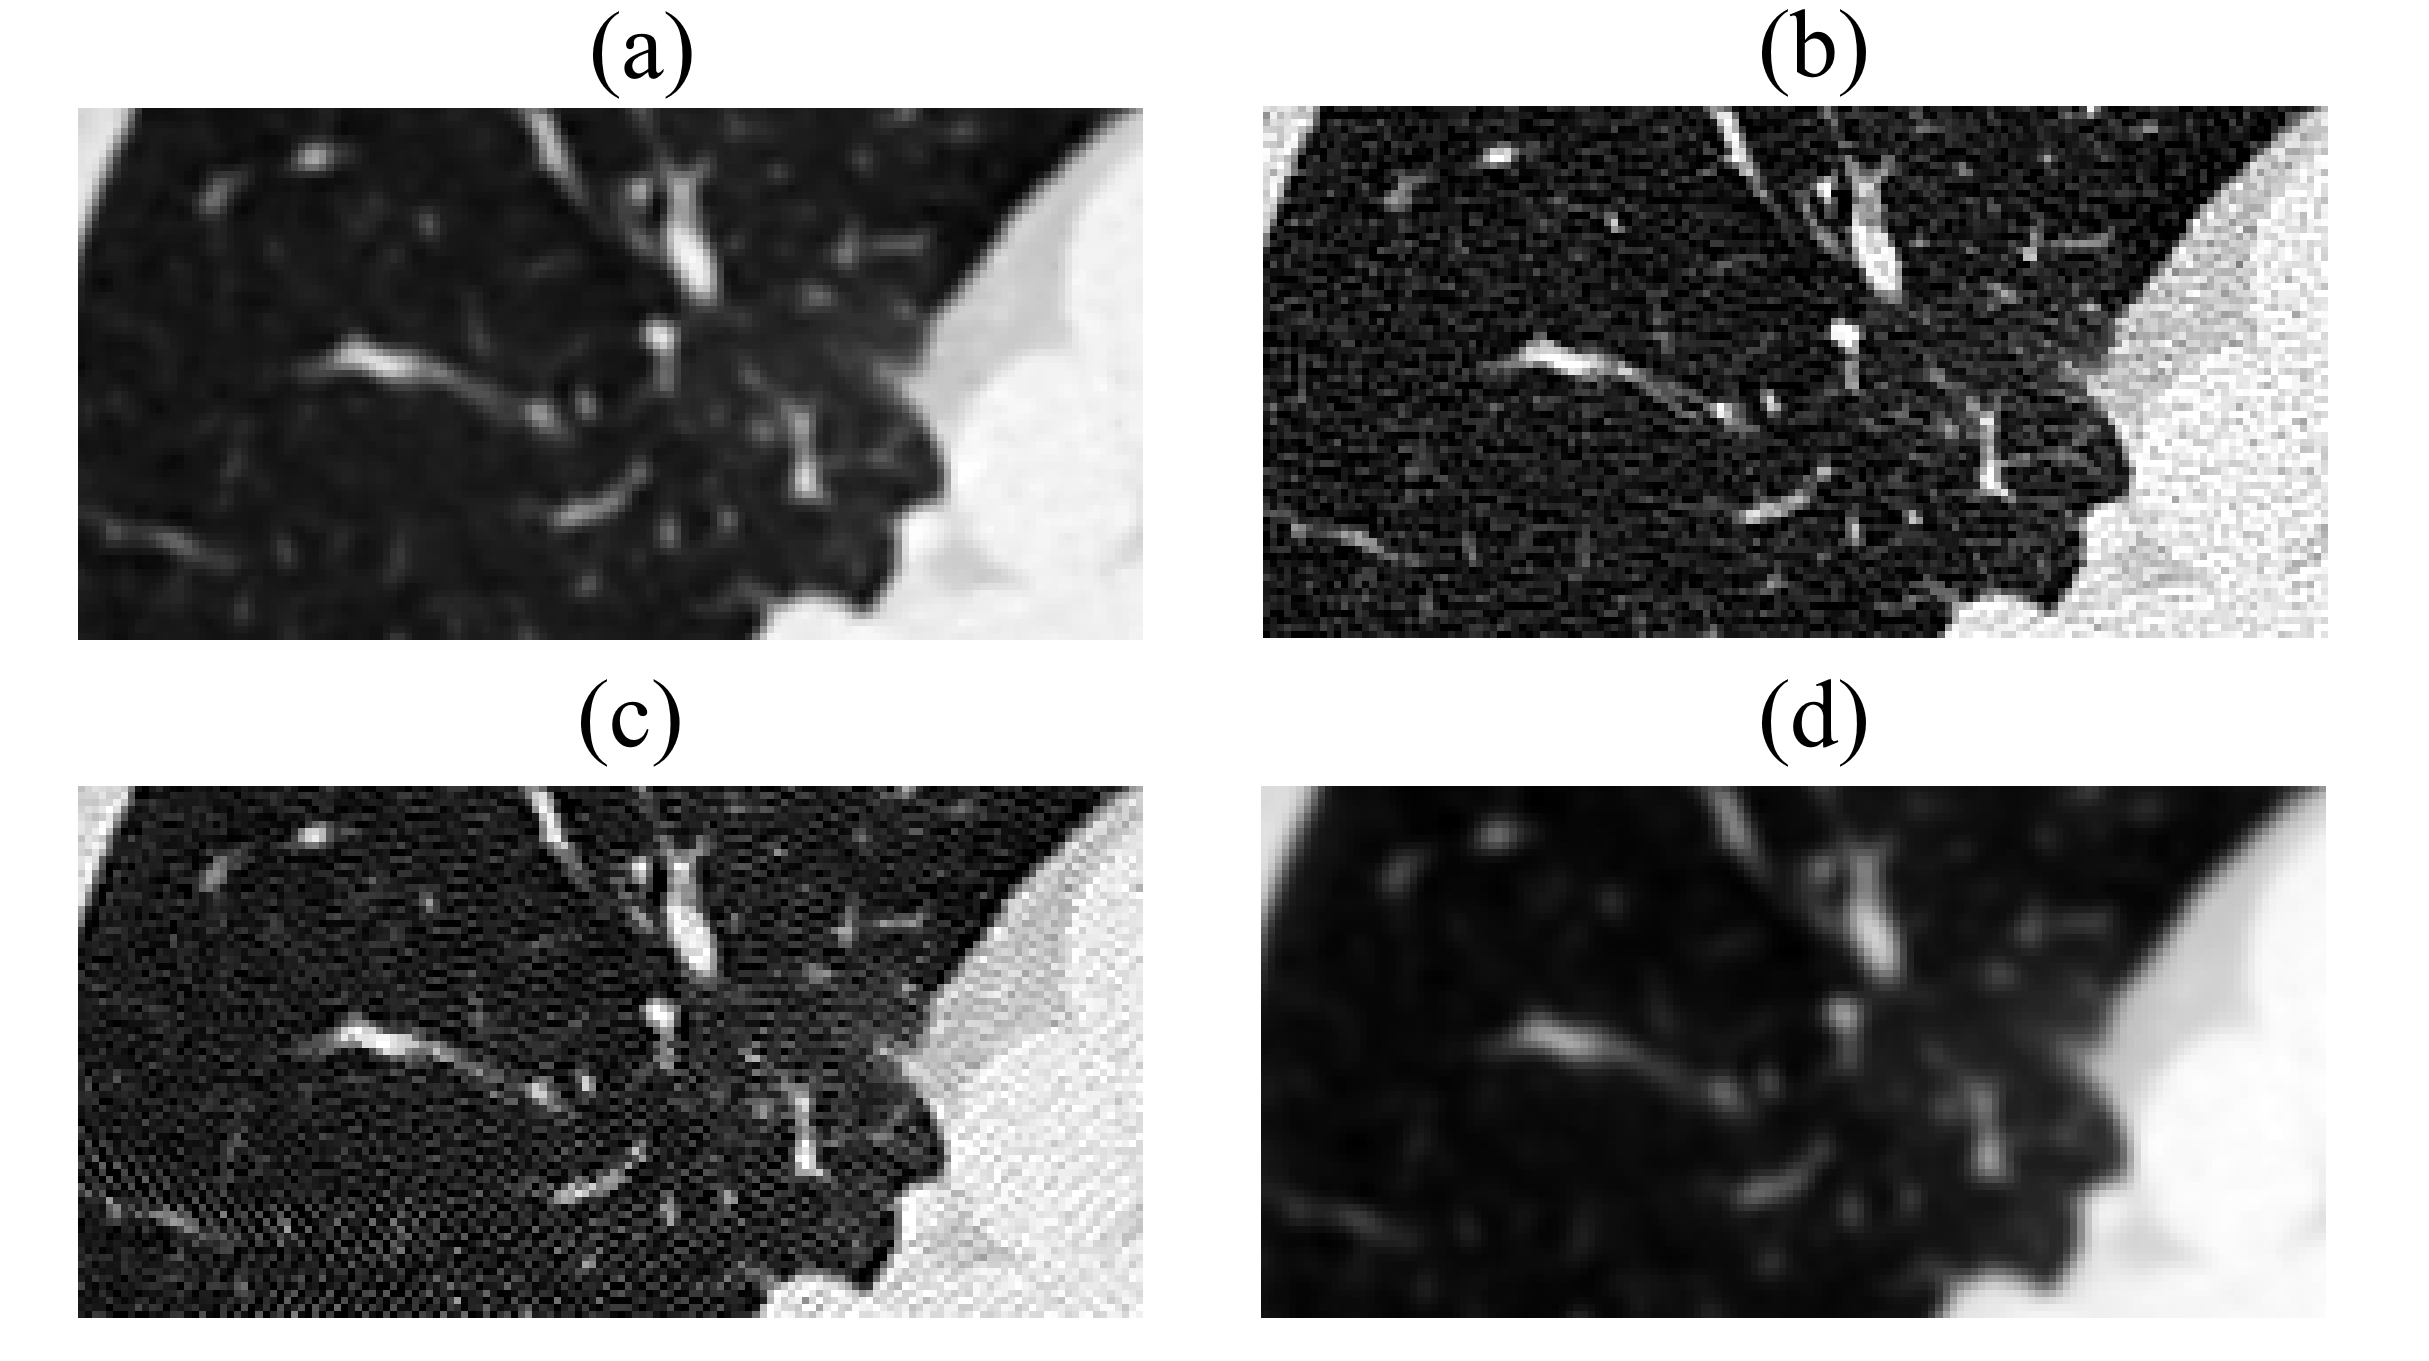
\includegraphics[width=\linewidth]{Dissertation/Figures/3_ct/4crops.png}%[width=7cm][width=7cm]
	\caption{\textbf{An example of paired CT slices (top row) and the effect of the augmentation by the proposed method (bottom row).} The top row contains original images: a slice reconstructed either with a smooth kernel (a) or sharp kernel (b). The bottom row shows augmented images: the top-left image processed by FBPAug with parameters $a=30,~b=3$ shifting it from smooth to sharp (c); the top-right image processed by FBPAug with parameters $a=-1,~b=0.7$ from sharp to smooth (d).}
	\label{fig:crops}
\end{figure}


\subsection{Cross-Domain Features Consistency}

We train all segmentation methods using the annotated dataset $S_s = \{ ( x_i, y_i ) \}_{i=1}^{N_s}$, where $x$ is a volumetric CT image, $y$ is a corresponding binary mask, and $N_s$ is the total size of training dataset. The dataset $S_s$ consists of images reconstructed with smooth kernels; we call it source dataset. We test all methods using the annotated dataset $S_t = \{ ( x_i, y_i ) \}_{i=1}^{N_t}$. The dataset $S_t$ consists of the $N_t$ images reconstructed with the sharp kernels; we call it target dataset. Although $S_t$ contains annotations, we use them only to calculate the final score.

Adaptation methods use additional paired dataset $S_2 = \{ ( x_i, \tilde{x}_i ) \}_{i=1}^{N_2}$, which has no annotations. However, every image $x \in S_2$ has a paired image $\tilde{x}$ reconstructed from the same sinogram but with a different kernel. Here, we assume that $x$ belongs to the source domain and $\tilde{x}$ belongs to the target domain.

Similar to the adversarial approaches (e.g., \cite{ganin2015unsupervised}), we propose to remove style-specific kernel information from the feature maps. However, we additionally exploit the paired nature of the unlabeled dataset $S_2$. Instead of the adversarial loss, we minimize the distance between feature maps of paired images. Let us denote feature extractor $H_f$, the part of segmentation model that maps input images $x$ into the feature space, and segmentation head $H_p$, the complement part of segmentation model that predicts binary mask $\hat{y} = H_p \left( H_f \left( x \right) \right)$. Further, we denote the feature vector for every image $x$ as $f$, $f = H_f (x; \: \theta_f)$. For the paired image $\tilde{x}$, we use the similar notation $\tilde{f}$.%In Figure~\ref{fig:method_schematic}, $H_f$ and $H_p$ correspond to the encoder and decoder parts of the model, respectively.

During the training, we minimize the sum of segmentation loss and distance between paired features ($f$ and $\tilde{f}$). Thus, the optimization problem is
\begin{align}
	\label{eq:f-consistency_opt}
	\begin{split}
		E (\theta_f, \theta_p) &= \sum_{i = 1}^{N_s} L_s (H_p(H_f (x_i; \: \theta_f); \: \theta_p), \: y_i) \: \\
		& + \: \alpha \sum_{j = 1}^{N_2} L_c (H_f (x_j; \theta_{f}), \: H_f (\tilde{x}_j; \theta_f)) \\
		& = \sum_{i = 1}^{N_s} L_s \left(\hat{y}_i ,\: y_i \right) \: + \: \alpha \sum_{j = 1}^{N_2} L_c (f_j,\: \tilde{f}_j ),  
	\end{split} \\
	(\hat{\theta}_f, \hat{\theta}_p) & = \argmin_{\theta_f, \theta_p} E(\theta_f, \theta_p),
\end{align}
where $L_s$ is the segmentation loss (Binary Cross-Entropy) and $L_c$ is the consistency loss. For the consistency loss, we use mean squared error (MSE) between paired feature maps. Parameter $\alpha$ regulates the trade-off between two objectives. We call this method \textit{F-Consistency} since it enforces the consistency between paired feature maps.

We present our method schematically in Figure~\ref{fig:method_schematic}(5) along with the competitive approaches, e.g., Domain Adversarial Neural Network (DANN) \cite{ganin2015unsupervised}. Note that we do not need any additional model as discriminator in DANN in the case of F-Consistency. The features are aggregated from the same encoder layers as in DANN.

\begin{landscape}
\begin{figure}[p]
	\centering
	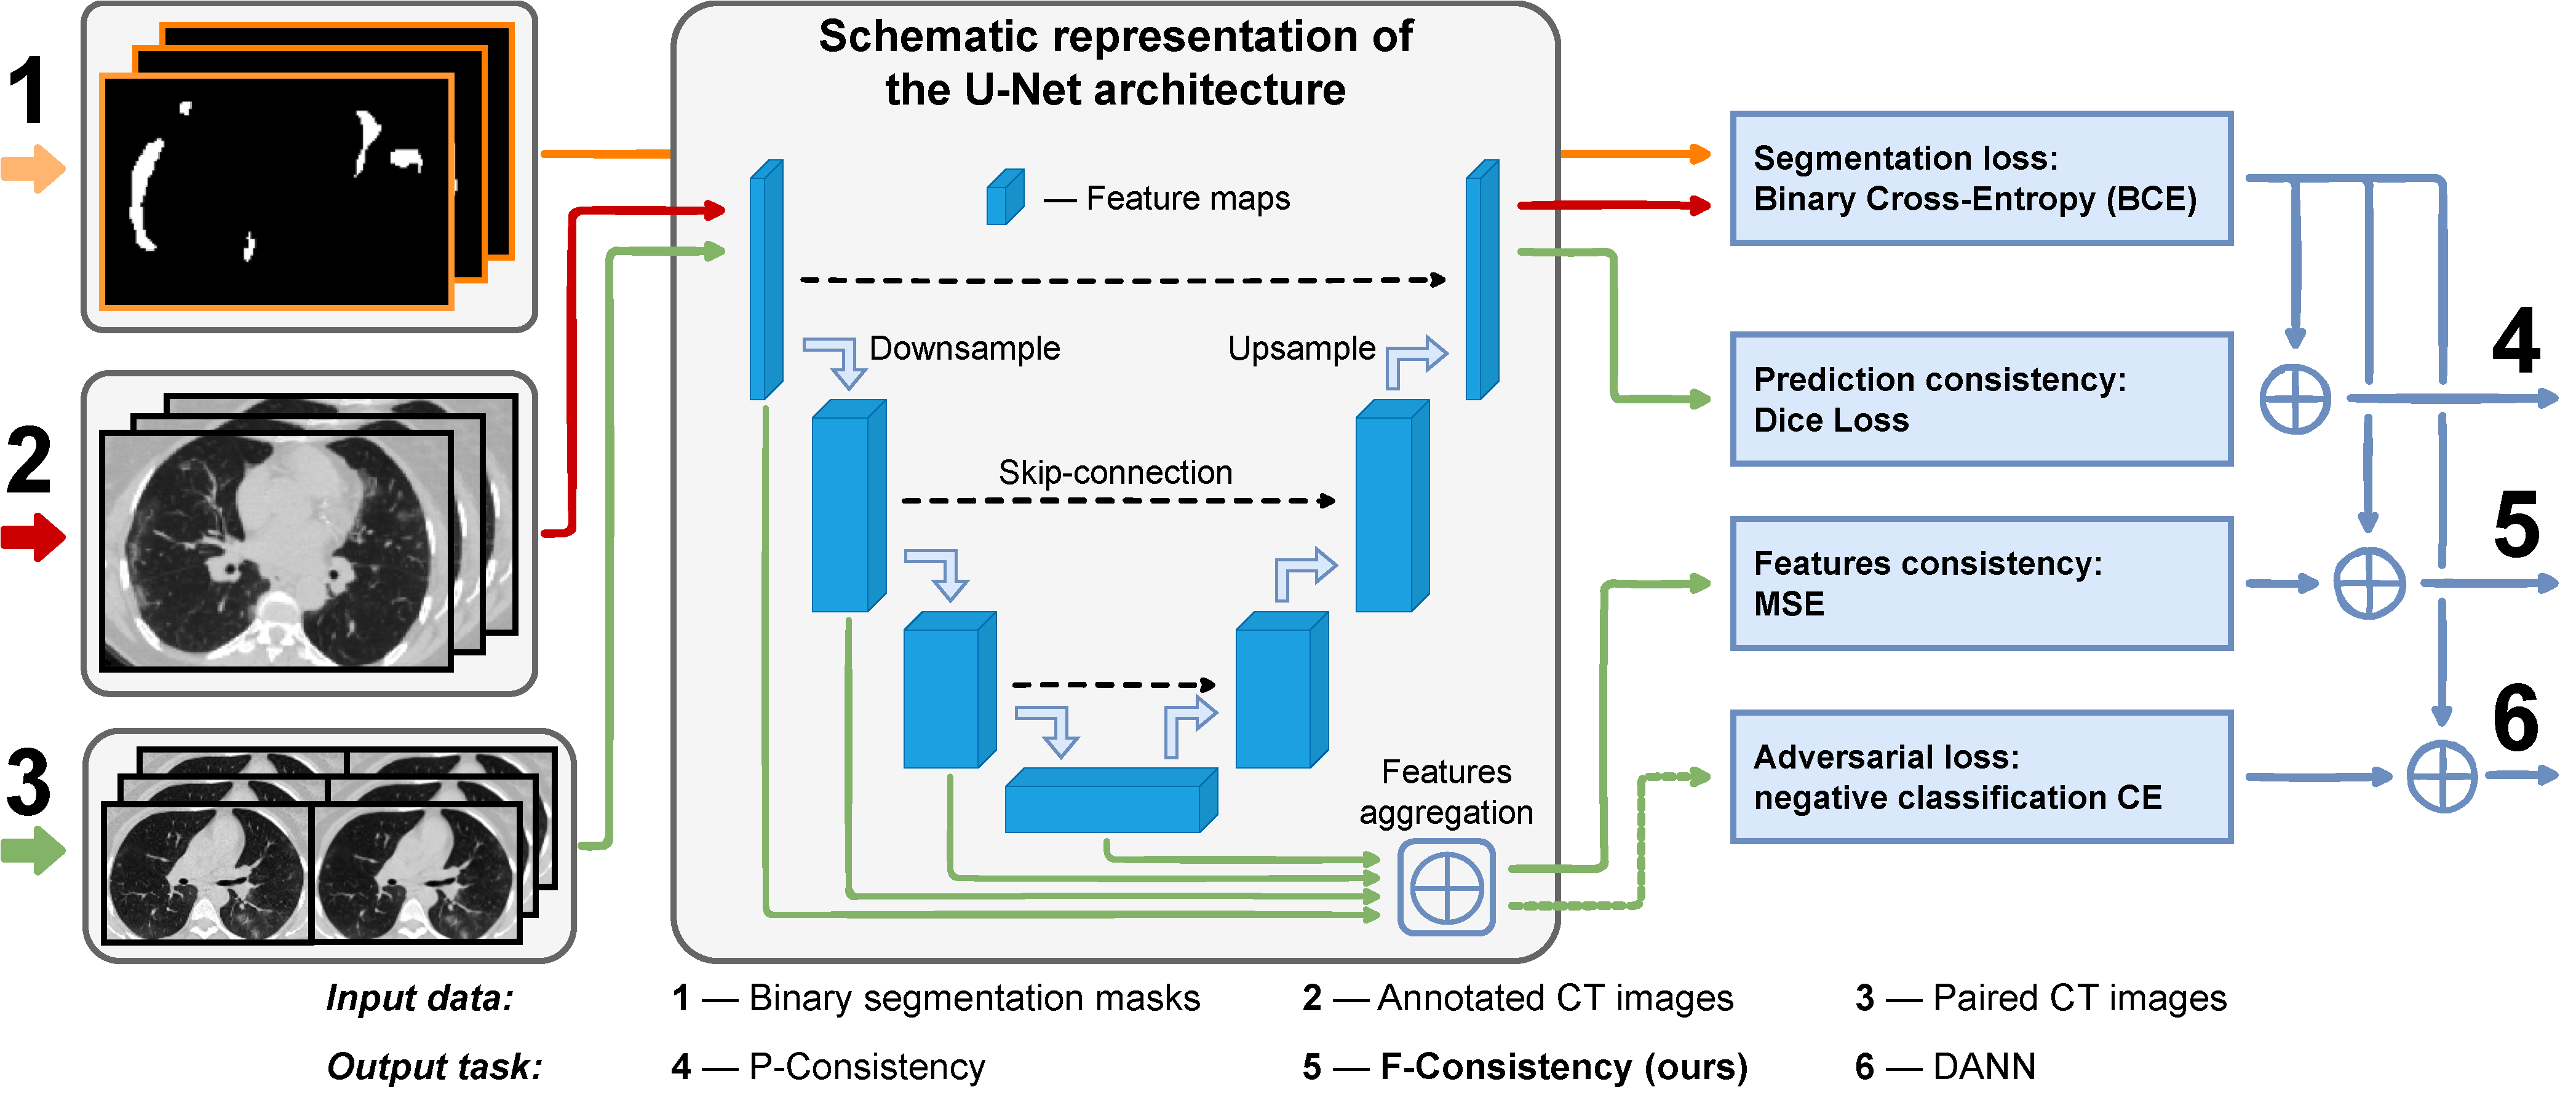
\includegraphics[width=\linewidth]{Dissertation/Figures/3_ct/method_schematic_4.pdf}
	\caption{Schematic representation of the proposed method, \textit{\textbf{F-Consistency}} (\textbf{5}), and its competitors, \textit{P-Consistency} (\textbf{4}) and \textit{DANN} (\textbf{6}). All methods build upon the same U-Net architecture, which we train to segment the COVID-19 binary mask (\textbf{1}) from the axial slices of chest CT images (\textbf{2}). These adaptation methods use unlabeled paired data (\textbf{3}) to improve the model performance on the target domain. We show the flow and different usage of the paired data in different methods with green.\label{fig:method_schematic}}
	%In the image, \textit{DANN} and \textit{F-Consistency} operate with the encoder layers but can be easily extended to the %decoder versions.
\end{figure}
\end{landscape}

\subsection{Cross-Domain Predictions Consistency}

A special case of F-Consistency is enforcing the consistency of paired predictions as the predictions are de facto the feature maps of the last network layer. This approach is proposed in \cite{orbes2019multi} also in the context of medical image segmentation. Further, we denote this method \textit{P-Consistency}. Visually, it could be compared with DANN and F-Consistency in Figure~\ref{fig:method_schematic}(4). The optimization problem is the same as in Equation~(\ref{eq:f-consistency_opt}), except $L_c$ is Dice Loss \cite{milletari2016v} and $f$ and $\tilde{f}$ are the last layer features, i.e., predictions.



\section{Data}

In our experiments, we use a combination of different datasets with chest CT images. The data could be divided into two subsets according to the experimental purposes. The first collection of datasets consists of images with annotated COVID-19 lesions, i.e., with binary masks of ground-glass opacity and consolidation. It serves to train the COVID-19 segmentation algorithms. The second collection consists of chest CT images which are reconstructed with different kernels but have no COVID-19 annotations. We filter the data into pairs of images reconstructed with the smooth and sharp kernels. This data is further used to adapt the models in an unsupervised manner.
% We detail every dataset of the segmentation collection in Section~\ref{ssec:data:segm}. 
% We detail the second collection in Section~\ref{ssec:data:paired}.


\subsection{Segmentation Data}

We use three publicly available datasets to train and test the segmentation algorithms: Mosmed-1110 \cite{morozov2020mosmeddata}, MIDRC \cite{tsai2021rsna}, and Medseg-9. We ensure that selected datasets contain original 3D chest CT imaging studies without third-party preprocessing artifacts. The images from the Mosmed-1110 and MIDRC datasets are reconstructed using smooth kernels, whereas Medseg-9 images have sharp reconstruction kernels. That allows us firstly to identify and then address the domain shift. We split the segmentation data into the source (COVID-train) and target (COVID-test) domains and describe them below. A summary of the segmentation datasets is presented in Table~\ref{tab:data_segm}.



%\begin{table}[H]
%	\centering
%	\caption{Summary of the segmentation datasets. {\textit{Effective size} means the number of annotated images after appropriate filtering.} \label{tab:data_segm}}
%	\newcolumntype{C}{>{\centering\arraybackslash}X}
%	\resizebox{\textwidth}{!}{%
%	\begin{tabularx}{\textwidth}{CCCCCC}
%		\toprule
%		\multirow{1.5}{*}{\textbf{Dataset}} & \multirow{1.5}{*}{\textbf{Source }}& \makecell{\textbf{Effective} \\ \textbf{Size}} & \multirow{1.5}{*}{\textbf{Kernels}} & \multirow{1.5}{*}{\textbf{Annotations}} &\multirow{1.5}{*}{ \textbf{Split}} \\
%		\midrule
%		\multirow{4}{*}{COVID-train} & \makecell{Mosmed-1110 \\ \cite{morozov2020mosmeddata}} & 50 & \makecell{unknown \\ smooth} & COVID-19 mask & \multirow{4}{*}{\makecell{5-fold \\ cross-val}} \\
%		\cmidrule(lr){2-5}
%		& \makecell{MIDRC \\ \cite{tsai2021rsna}} & 112 & \makecell{B/L/BONE/ \\ STANDARD \\ (smooth)} & COVID-19 mask & \\
%		\midrule
%		COVID-test & Medseg-9 & 9 & \makecell{unknown \\ sharp} & \makecell{COVID-19 mask, \\ lungs mask} & \makecell{hold-out \\ test} \\
%		\bottomrule
%	\end{tabularx}}
%\end{table}


\begin{table}[h]
	\centering
	\caption{Summary of the segmentation datasets.\label{tab:data_segm}}
	
	%\resizebox{\textwidth}{!}{%
		\begin{tabular}{c c c c c c}
			\toprule
			Dataset & Source & Size & Kernels & Annotations & Split \\
			\midrule
			\multirow{2}{*}[-1.0em]{\textit{COVID-train}} & Mosmed-1110 & 50 & \makecell{unknown \\ smooth} & COVID-19 & \multirow{2}{*}[-1.5em]{\makecell{5-fold \\ cross-val}} \\
			\cmidrule(lr){2-5}
			& MIDRC & 112 & \makecell{B/L/BONE/ \\ STANDARD \\ (smooth)} & COVID-19 & \\
			\midrule
			\textit{COVID-test} & Medseg-9 & 9 & \makecell{unknown \\ sharp} & \makecell{COVID-19, \\ lungs} & \makecell{hold-out \\ test} \\
			\bottomrule
			
	\end{tabular}%}
\end{table}


\textbf{Mosmed-1110.} This dataset consists of $1110$ chest CT scans collected in Moscow clinics during the first months of $2020$ \cite{morozov2020mosmeddata}. Scanning was performed on \textit{Canon (Toshiba) Aquilion 64} units using the standard scanner's protocol: inter-slice distance of $0.8$ mm and smooth reconstruction kernels in particular. However, the public version of Mosmed-1110 contains every $10th$ slice of the original series, which makes the resulting slice distance equal to $8.0$ mm. Additionally, the $50$ series have annotated binary masks depicting COVID-19 lesions (ground-glass opacity and consolidation). We use only these $50$ images in our experiments.
% Also, as one of the preprocessing steps, we crop images to lung masks. However, lungs are not annotated in the dataset. We obtain the lung masks using a standalone algorithm; see details in Section~\ref{ssec:exp:covid_segm}.


\textbf{MIDRC.} MIDRC-RICORD-1a is the publicly available dataset that contains $120$ chest CT studies \cite{tsai2021rsna}. The total number of volumetric series is $154$. According to the DICOM entries, {all} images have smooth reconstruction kernels. The dataset contains at least $12$ paired images (without considering the studies that contain more than two series). But we do not use these pairs to enforce consistency since both images have smooth kernels. Also, we use only the images that have non-empty annotations. The images that have empty binary masks of COVID-19 are discarded from both of the datasets. The resulting training dataset consists of $112$ volumetric images with smooth kernels.
% Also, the original dataset does not contain annotated lung masks. Therefore, similarly to \textit{Mosmed-1110}, we predict the lung masks with our standalone algorithm.
% All studies were performed using \textit{Phillips} scanner.

\textbf{Medseg-9.} MedSeg website ({\url{https://medicalsegmentation.com/covid19/}} (visited on 08/24/2022)) shares a publicly available dataset with $9$ annotated chest CT images from {Radiopaedia.org} ({\url{https://radiopaedia.org/articles/covid-19-3}} (visited on 08/19/2024)), all reconstructed with sharp kernels.


\subsection{Paired Images Data}
%\label{ssec:data:paired}

To train and evaluate the consistency of the segmentation algorithms, we use two sources of paired data. The first source is a publicly available dataset Cancer-500 \cite{morozov2021simplified}. But the Cancer-500 dataset does not contain COVID-19 cases. Thus, to properly evaluate the consistency of COVID-19 segmentation algorithms, we use the second source of private data that contains COVID-19 cases. 

From Cancer-500, we build the Paired-public dataset and use it only to train the segmentation algorithms in an unsupervised manner. Then, we build the Paired-private dataset from our private data. Besides training, we use this dataset to evaluate the consistency scores since it contains the segmentation target (COVID-19 lesions). The summary of the paired datasets is presented in Table~\ref{tab:data_paired}.



%\begin{table}[H]
%	\caption{Summary of the datasets with paired images.\label{tab:data_paired}}
%	\newcolumntype{C}{>{\centering\arraybackslash}X}
%	\begin{tabularx}{\textwidth}{CCCC}
%		\toprule
%		\textbf{Dataset} &\textbf{ Kernel Pair} (\textbf{smooth}/\textbf{sharp}) & \textbf{Training} & \textbf{Testing Pairs }\\
%		\midrule
%		\multirow{2}{*}{\makecell{Paired-public \\ \citep{cancer500}}} & FC07/FC55 & 22 & 0 \\
%		& FC07/FC51 & 98 & 0 \\
%		\midrule
%		\multirow{4}{*}{Paired-private} & FC07/FC55 & 60 & 20 \\
%		& FC07/FC51 & 30 & 11 \\
%		& SOFT/LUNG & 30 & 10 \\
%		& STANDARD/LUNG & 30 & 10 \\
%		\bottomrule
%	\end{tabularx}
%\end{table}


\begin{table}[h]
	\centering
	\caption{Summary of the datasets with paired images.\label{tab:data_paired}}
	\resizebox{\textwidth}{!}{%
		\begin{tabular}{c c c c}
			\toprule
			Dataset & Kernel pair (\textit{smooth}/\textit{sharp}) & Training & Testing pairs \\
			\midrule
			\multirow{2}{*}{\makecell{Paired-public \\ \cite{morozov2021simplified}}} & FC07/FC55 & 22 & 0 \\
			& FC07/FC51 & 98 & 0 \\
			\midrule
			\multirow{4}{*}{Paired-private} & FC07/FC55 & 60 & 20 \\
			& FC07/FC51 & 30 & 11 \\
			& SOFT/LUNG & 30 & 10 \\
			& STANDARD/LUNG & 30 & 10 \\
			\bottomrule
	\end{tabular}}
\end{table}


Both datasets do not contain any COVID-19 annotations and we do not need them since we use these datasets in unsupervised training.


\textbf{Paired-public dataset.} We build the Paired-public using a publicly available dataset, Cancer-500 \cite{morozov2021simplified}. The data was collected from $536$ randomly selected patients of Moscow clinics in 2018. All original images were obtained using a Toshiba scanner and reconstructed with FC07, FC51, or FC55 kernels. Here, FC07 is a smooth reconstruction kernel, whereas FC51 and FC55 are sharp kernels. From $536$ studies, we extracted $120$ pairs, comparing the shape and acquisition time of the corresponding DICOM series and filtering contrast-enhanced cases. As a result, the Paired-public dataset consists of $98$ FC07/FC51 and $22$ FC07/FC55 pairs. We use this dataset to train the domain adaptation algorithms on paired images. % 970 series. Details are provided in Tab.

However, the Paired-public dataset does not contain COVID-19 cases, since it was collected before the pandemic. The latter observation limits using this dataset to evaluate the consistency. Otherwise, we evaluate the quality of COVID-19 segmentation algorithms using images with no COVID-19 lesions, either evaluating the consistency of noisy or false positive predictions. For the same reason, one should also be careful using this data to enforce the consistency in the last network layers, e.g., in P-Consistency. The data without COVID-19 lesions can force the network to output trivial predictions.

Therefore, we introduce a private dataset for the extended consistency evaluation.


\textbf{Paired-private.} From the private collection of the chest CT images, we filter out $181$ pairs to create the Paired-private dataset. These images were initially collected from Moscow outpatient clinics during the year 2020. Scanning was performed on the Toshiba and GE medical systems units using diverse settings. We select the four most frequent kernel pairs with a total of six unique reconstruction kernels: FC07, FC51, FC55, LUNG, SOFT, and STANDARD. The distribution of these kernel pairs is given in Table~\ref{tab:data_paired}.

These images contain COVID-19 lesions, therefore we use the Paired-private dataset both for training and evaluation. The wider variety of kernels also allows us to test the generalization of algorithms to unseen kernels. More specifically, we consider kernels LUNG, SOFT, and STANDARD in the Paired-private dataset to be unseen for the model trained on Paired-public data or only FC07, FC51, and FC55 kernels (excluding the rest).


\section{Experiments}

\subsection{Segmentation model}

For all our experiments, we use a  slightly modified 2D U-Net \cite{ronneberger2015u}, introducing the standard architectural modifications, such as replacing every convolution layer with the Residual Block \cite{he2016deep}. We prefer the 2D model to 3D since in the Mosmed-1110 dataset images have an 8 mm inter-slice distance and the inter-slice distance of Covid-private images is in the range from 0.8 mm to 1.25 mm. Furthermore, the 2D model shows performance almost equal to the performance of the 3D model for COVID-19 segmentation \cite{goncharov2021ct}.% We also note that all considered methods are independent of the architecture choice.

\textbf{Preprocessing.} Before passing to the segmentation model, we apply the same preprocessing pipeline to all CT images. Preprocessing consists of four steps. (i) We rescale a CT image to have $1.75 \times 1.75$ mm axial resolution {using linear interpolation}. (ii) Then, the intensity values are clipped to the minimum of $-1000$ Hounsfield units (HU) and a maximum of $300$ HU. (iii) The resulting intensities are min-max-scaled to the $[0; 1]$ range. (iv) Finally, we crop the resulting image to the automatically generated lung mask.

We generate the lung mask by training a standalone CNN segmentation model. The training procedure and architecture are reproduced from \cite{goncharov2021ct}. The training of the lung segmentation model involves two external chest CT datasets: LIDC-IDRI~\cite{lidc} and NSCLC-Radiomics~\cite{nsclc1,nsclc2}. These datasets have no intersection with the other datasets used to train the COVID-19 segmentation models, so there is no possible data leak. The trained lung segmentation model achieves about $0.98$ Dice Score both on the cross-validation and on the Medseg-9 dataset (it contains annotated lung masks). The latter result indicates that the lung segmentation model is robust to different kinds of domain shift and, moreover to the appearance of novel lesions (COVID-19).

\textbf{Training details.} We train all models for 25000 iterations using Adam~\cite{kingma2014adam} optimizer with the default parameters and an initial learning rate of $10^{-4}$. Every 6000 iterations the learning rate is multiplied by $0.2$. Each iteration contains 32 randomly sampled 2D axial slices. Training of the plain segmentation model and similarly F-Consistency takes approximately 8 hours on Nvidia GTX 1080 (8 GB) (Santa Clara, CA, USA). Training of DANN and FBPAug takes 12 and 30 hours, respectively, in the same setting. The inference time is approximately 5 -- 10 seconds depending on the image size and it is the same for all methods. As a loss function, we use binary cross-entropy (BCE).

% With probability $0.5$ we rotate an image by multiply of $90$ degrees and flip an image horizontally or vertically.


\subsection{FBPAug experiments and results}

We compare the proposed method with three standard augmentations: gamma transformation (Gamma)~\cite{tureckova2020improving}, additive Gaussian noise (Noise), and random windowing (Windowing), the technique proposed in~\cite{kloenne2020domain}. As a baseline method, we train a network without any intensity augmentations (Baseline).

\textbf{Gamma} augments images using the following intensity transformation:

\[
	\hat{I}(x, y) = \left(\frac{I(x, y) - m}{M - m}\right)^\gamma \cdot(M - m) + m,
\]

\noindent
where $M = \max(I(x, y))$, $m=\min(I(x, y))$ with a parameter $\gamma$, such that we randomly sample the logarithm of $\gamma$ from $\mathcal{N}(0, 0.2)$. 

\textbf{Noise} is the additive gaussian noise drown from $\mathcal{N}(0, 0.1)$. 

\textbf{Windowing}  makes use of the fact that different tissue has diferent attenuation coefficient. We uniformly sample the center of the window $c$ from $[-700, -500]$ HU  and the width of the window $w$ from $[1300, 1700]$ HU. Then we clip the image to the $[c - w/2, c + w/2]$ HU range.

\textbf{FBPAug} parameters were sampled as follows. We uniformly sample $a$ from $[10.0, 40.0]$ and  $b$ from $[1.0, 4.0]$ in sharpening case and $a$ from $[-1.0, 0]$, $b$ from $[0.1, 1.0]$ in smoothing case.

Table~\ref{tab:fbpaug_res} summarizes our FBPAug results. First, experiments on COVID-test show that segmentation quality almost does not differ for compared methods. The three best augmentation approaches are not significantly different (Wilcoxon test P-values are 0.71 for FBPAug vs. Gamma and 0.17 for FBPAug vs. Windowing). Thus, our method at least does not harm segmentation performance and performs on-par with the best reported method for this dataset~\cite{goncharov2021ct}.



\begin{table}[h]
	\centering
	\caption{FBPAug comparison results. Numbers are mean (std) obtained on 3-fold cross-validation. Results for \textit{COVID-test} are segmentation Dice score compared with ground truth; results for \textit{Paired-private} are predictions agreement (between paired images) measured using Dice score.}
	% The best results in each column are shown in bold.
	\resizebox{\textwidth}{!}{%
	\begin{tabular}{lccccc}%{| l | c | c | c | c | c |}
		% \cmidrule(lr){2-5}
		\toprule
		& Baseline & FBPAug & Gamma & Noise & Windowing \\
		
		\midrule
		% COVID-test          &$~0.56 ~(0.23)~$  &    $~0.59 ~(0.22)~$&    $\bf~0.61 ~(0.19)~$&    $~0.56 ~(0.21)~$&    $~0.59 ~(0.18)~$\\
		% Paired-private         &$0.54 ~(0.27)$  &    $\bf0.92 ~(0.05)$&    $0.68 ~(0.21)$&    $0.79 ~(0.13)$&    $0.63 ~(0.23)$\\
		
		COVID-test          &$~0.56 ~(0.23)~$  &    $\mathbf{~0.62 ~(0.18)~}$&    $~0.61 ~(0.19)~$&    $~0.56 ~(0.21)~$&    $~0.59 ~(0.18)~$\\
		Paired-private         &$0.54 ~(0.27)$  &    $\mathbf{0.92 ~(0.05)}$&    $0.68 ~(0.21)$&    $0.79 ~(0.13)$&    $0.63 ~(0.23)$\\
		
		\bottomrule
	\end{tabular}}
	\label{tab:fbpaug_res}
\end{table}



Next, we observe a significant disagreement in predictions on paired (\textit{smooth} and \textit{sharp}) images for all methods, except FBPAug (Wilcoxon test P-values for FBPAug vs. every other method are all less than $10^{-6}$). For FBPAug and its best competitor, we show a Bland-Altman plot, comparing GGO volume estimates; see Figure~\ref{fig:bland-altman}. We note that the predictions of FBPAug model agree independent of the volume of GGO. Qualitatively, the improved predictions consistency of our proposed FBPAug on the images with smooth and sharp kernels could be seen in Figure~\ref{fig:fbpaug_pred}.

\begin{figure}[h]
	\centering
	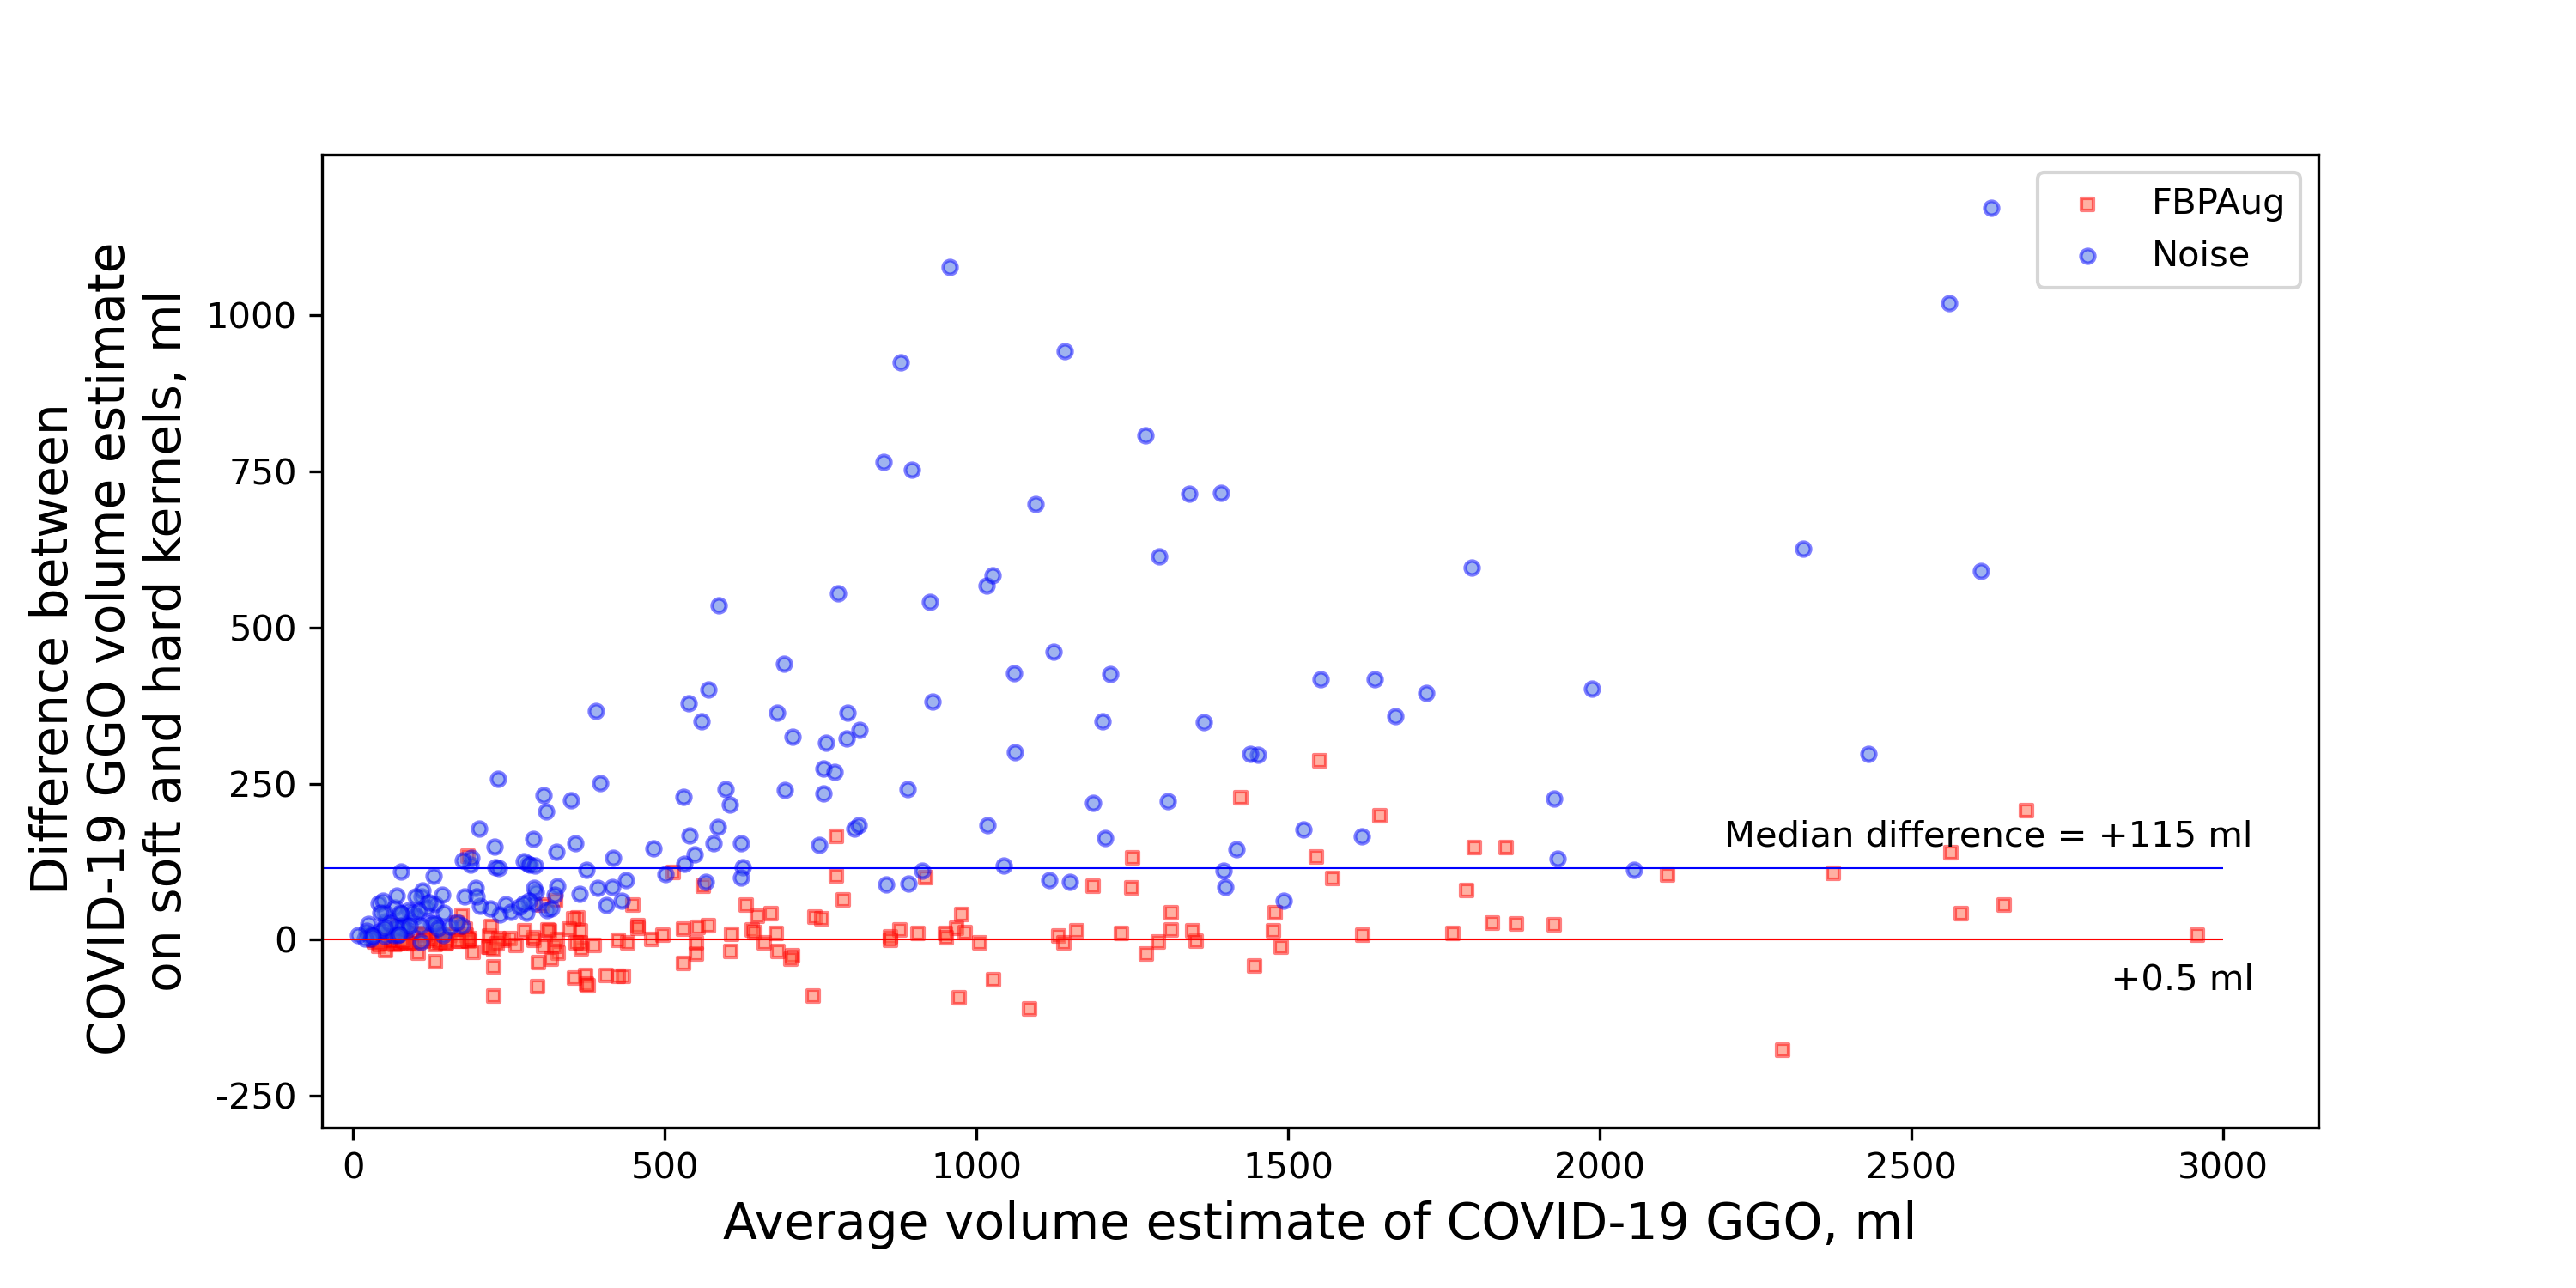
\includegraphics[width=\textwidth]{Dissertation/Figures/3_ct/bland-altman.png}
	\caption{Bland-Altman plot showing prediction agreement using FBPAug (proposed augmentation, red) and next best competitor (Gaussian noise, blue).}
	\label{fig:bland-altman}
\end{figure}

\begin{figure}[h]
	\centering
	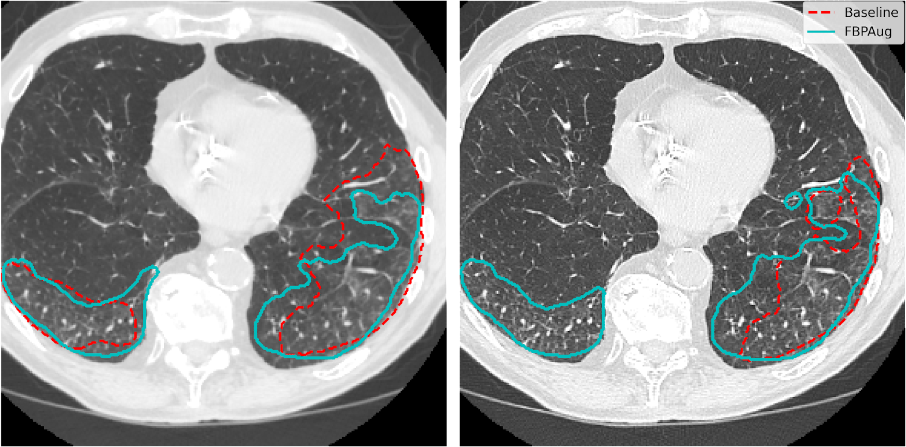
\includegraphics[width=\textwidth]{Dissertation/Figures/3_ct/contours_new.png}
	\caption{Example FBPAug predictions. Left -- image reconstructed with a \textit{smooth} kernel. Right -- image reconstructed with a \textit{sharp} kernel from the same sinogram.}
	\label{fig:fbpaug_pred}
\end{figure}


\subsection{F-consistency experiments and results}

We compare some of the key results statistically using a one-sided Wilcoxon signed-rank test. We report p-values in two testing setups: $p_1$ -- comparing five mean values after cross-validation, and $p_2$ -- comparing Dice Score on every image as an independent sample.


\textbf{Methods comparison.} To begin with, we show the existence of the domain shift problem within the COVID-19 segmentation task. The Dice Score of the baseline model on the COVID-test dataset is lower than the cross-validation score on the COVID-train dataset, $0.56$ against $0.60$. Also, this score is significantly lower than $0.64$ achieved by our adaptation method $\left(p_1 < 0.05,\: p_2 < 10^{-4} \right)$. Results could be found in Table~\ref{tab:res_final} comparing row Baseline to the others. For all adaptation methods, we observe an increase in the consistency score and segmentation quality on the target domain. Moreover, all methods maintain their quality on the source domain compared to Baseline.



%\begin{table}[H]
%	\caption{Comparison of all considered methods. The adaptation methods are trained using all training kernel pairs of the Paired-private dataset. F-/P-Cons stand for F-/P-Consistency, where F-Consistency is our proposed method. All results are Dice Scores in the format \textit{mean} $\pm$ \textit{std} calculated from $5$-fold cross-validation. We highlight the best scores in every column in \textbf{bold}.}
%	\begin{adjustwidth}{-\extralength}{0cm}
%		\newcolumntype{C}{>{\centering\arraybackslash}X}
%		\begin{tabularx}{\fulllength}{lCCCCCCC}
%			\toprule
%			
%			& \multirow{2.5}{*}{\textbf{COVID-train}} & \multirow{2.5}{*}{\textbf{COVID-test}} & \multicolumn{5}{c}{\textbf{Paired-Private} \textbf{Consistency}} \\
%			\cmidrule(lr){4-8}
%			& & & \textbf{FC07/55} & \textbf{FC07/51} & \textbf{SOFT/LUNG} & \textbf{STAND/LUNG}  & \textbf{Mean} \\
%			
%			
%			\midrule
%			Baseline & $\mathbf{0.60 \pm 0.04}$ & $0.56 \pm 0.03$ & $0.52 \pm 0.06$ & $0.39 \pm 0.07$ & $0.58 \pm 0.08$ & $0.28 \pm 0.05$ & $0.46 \pm 0.05$\\
%			
%			\cmidrule{1-8}
%			
%			FBPAug & $0.59 \pm 0.04$ & $0.62 \pm 0.03$ & $0.80 \pm 0.02$ & $0.71 \pm 0.03$ & $0.85 \pm 0.01$ & $0.65 \pm 0.03$ & $0.76 \pm 0.02$ \\
%			
%			
%			\cmidrule{1-8}
%			
%			%DANN (Dec) & $.57 \pm 0.04$ & $.61 \pm 0.04$ &  $.61 \pm 0.02$ & $.49 \pm 0.04$ & $.58 \pm 0.03$ & $.31 \pm 0.05$ & $.52 \pm 0.01$ \\
%			
%			%\cmidrule{1-8}
%			
%			DANN  & $0.58 \pm 0.05$ & $\mathbf{0.64 \pm 0.02}$ & $0.84 \pm 0.02$ & $0.70 \pm 0.02$ & $\mathbf{0.86 \pm 0.03}$ & $0.66 \pm 0.06$ & $0.78 \pm 0.02$ \\
%			
%			\cmidrule{1-8}
%			
%			P-Cons & $0.59 \pm 0.04$ & $0.61 \pm 0.01$ & $0.65 \pm 0.05$ & $0.60 \pm 0.02$ & $0.77 \pm 0.01$ & $0.47 \pm 0.04$ & $0.63 \pm 0.03$\\
%			
%			\cmidrule{1-8}
%			
%			
%			%F-Cons (Dec) & $\mathbf{.60 \pm 0.03}$ & $.58 \pm 0.02$ & $.62 \pm 0.05$ & $.54 \pm 0.03$ & $.75 \pm 0.01$ & $.40 \pm 0.06$ & $.58 \pm 0.02$ \\
%			
%			%\cmidrule{1-8}
%			
%			F-Cons &  $0.57 \pm 0.03$ & $\mathbf{0.64 \pm 0.03}$ & $\mathbf{0.88 \pm 0.01}$ & $\mathbf{0.72 \pm 0.04}$ & $0.83 \pm 0.02$ & $\mathbf{0.70 \pm 0.05}$ & $\mathbf{0.80 \pm 0.01}$ \\
%			
%			\bottomrule
%		\end{tabularx}
%		\label{tab:res_final}
%	\end{adjustwidth}
%\end{table}


\begin{table}[h]
	\centering
	\caption{Comparison of all considered methods, trained using all kernel pairs of the Paired-private dataset. All results are Dice Scores in the format \textit{mean (std)}.}
	\label{tab:res_final}
	%\resizebox{\textwidth}{!}{%
		\begin{tabular}{lcccccc}
			\toprule
			& \multirow{2.5}{*}{\shortstack{COVID-\\test}} & \multicolumn{5}{c}{Paired-private consistency} \\
			\cmidrule(lr){3-7}
			& & FC07/55 & FC07/51 & soft/lung & stnd/lung & mean \\
			\midrule
			
			Baseline & 0.56(0.03) & 0.52(0.06) & 0.39(0.07) & 0.58(0.08) & 0.28(0.05) & 0.46(0.05) \\
			
			\cmidrule{1-7}
			
			P-Cons & 0.61(0.01) & 0.65(0.05) & 0.60(0.02) & 0.77(0.01) & 0.47(0.04) & 0.63(0.03) \\
			
			\cmidrule{1-7}
			
			FBPAug & 0.62(0.03) & 0.80(0.02) & 0.71(0.03) & 0.85(0.01) & 0.65(0.03) & 0.76(0.02) \\
			
			\cmidrule{1-7}
			
			DANN & \textbf{0.64(0.02)} & 0.84(0.02) & 0.70(0.02) & \textbf{0.86(0.03)} & 0.66(0.06) & 0.78(0.02) \\		
			
			\cmidrule{1-7}
			
			F-Cons & \textbf{0.64(0.03)} & \textbf{0.88(0.01)} & \textbf{0.72(0.04)} & 0.83(0.02) & \textbf{0.70(0.05)} & \textbf{0.80(0.01)} \\
			
			\bottomrule
		\end{tabular}%}
\end{table}


% Further, we compare FBPAug to the best adaptation methods since it is a straightforward solution to the domain shift problem caused by the difference in the reconstruction kernels. Although FBPAug achieves comparable results on the target domain, F-Consistency outperforms it in terms of the average consistency score, $0.80$ Dice Score against $0.76$ $\left(p_1 < 0.05,\: p_2 < 10^{-5}\right)$. The results are also in Table~\ref{tab:res_final}, row FBPAug.

We compare P-Consistency (which operates with the last layer of decoder) with F-Consistency and show it resulting in the significantly lower consistency score, $0.63$ against $0.80$ $\left(p_1 < 0.05,\: p_2 < 10^{-10}\right)$. Thus, our findings align with the message of~\cite{zakazov2021anatomy} that the encoder layers contain more domain-specific information than the decoder ones.

F-consistency outperforms DANN. Although both methods score similar in target Dice Score, F-Consistency has an advantage over DANN in the consistency score: $0.80$ against $0.78$ $\left(p_1 < 0.05,\: p_2 < 10^{-2}\right)$. Our intuition here is F-Consistency explicitly enforces features alignment, while DANN enforces features to be indistinguishable for the discriminator. The latter differently impact the consistency score, and F-Consistency performs better.

We conclude comparison of the methods with the qualitative analysis. In Figure~\ref{fig:test_preds}, one could find examples of the Baseline, FBPAug, DANN, and F-Consistency predictions on the COVID-test dataset and compare them with the ground truth. All adaptation methods perform similar to the ground truth with minor inaccuracies, while Baseline gives massive false positive predictions on the unseen domain.%With the quantitative analysis above, these observations highlight the relevance of the domain adaptation problem in the COVID-19 segmentation task.

\begin{figure}[h]
	\centering
	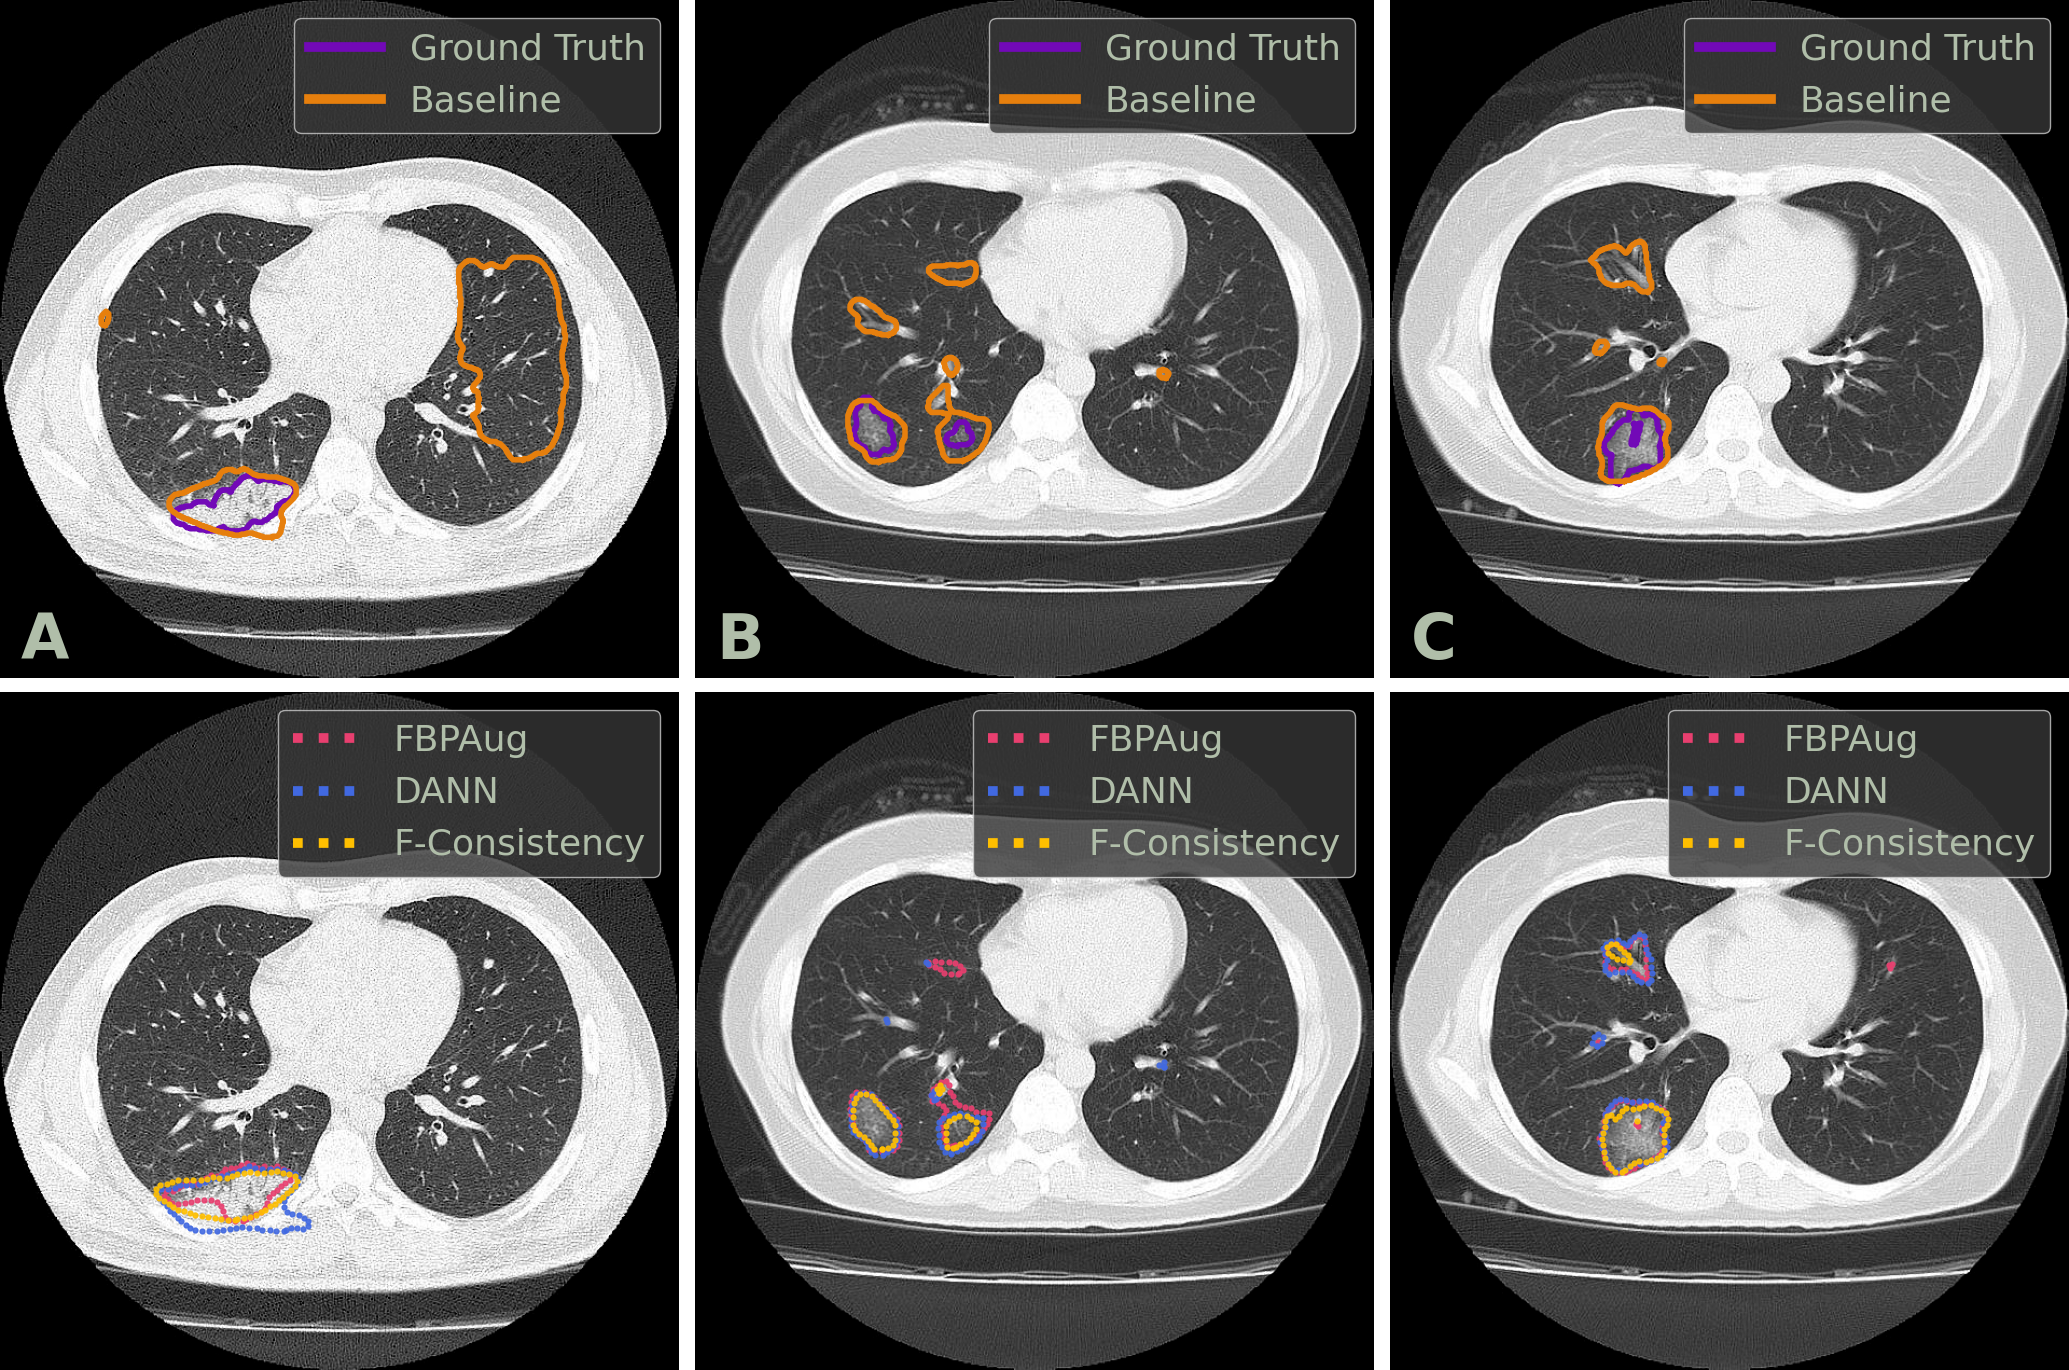
\includegraphics[width=\textwidth]{Dissertation/Figures/3_ct/test_preds.png}
	\caption{Examples of three axial CT slices (columns A, B, and C) from the COVID-test dataset with the corresponding predictions and ground truth annotations.}% Three columns, denoted \textbf{A}, \textbf{B}, and \textbf{C}, contains three unique slices.}% The top row contains the contours of the ground truth and baseline prediction. The bottom row contains the contours of the adaptation methods' predictions. DANN and F-Consistency correspond to DANN and F-Cons from Table~\ref{tab:res_final}, respectively.}
	\label{fig:test_preds}
\end{figure}

In Figure~\ref{fig:consistency_preds}, we visualize predictions of the same four methods on the paired images from the Paired-private dataset. For the Baseline, we observe an extreme inconsistency (Figure~\ref{fig:consistency_preds}~A) and massive false positive predictions in healthy lung tissues (Figure~\ref{fig:consistency_preds}~D) and even outside lungs (Figure~\ref{fig:consistency_preds}~B). For the adaptation methods, their predictions are visually more consistent inside every pair. Despite the high consistency scores, FBPAug and DANN output more aggressive predictions. FBPAug predicts motion artifacts near the body regions (Figure~\ref{fig:consistency_preds}~A) and triggers similarly to the Baseline on healthy lung tissues (Figure~\ref{fig:consistency_preds}~B). DANN is more conservative but triggers on the consolidation-like tissues (Figure~\ref{fig:consistency_preds}~C,~D). However, without the ground truth annotations on the paired data, we refer to this analysis as a discussion.

\begin{landscape}
\begin{figure}[p]
	% \centering
	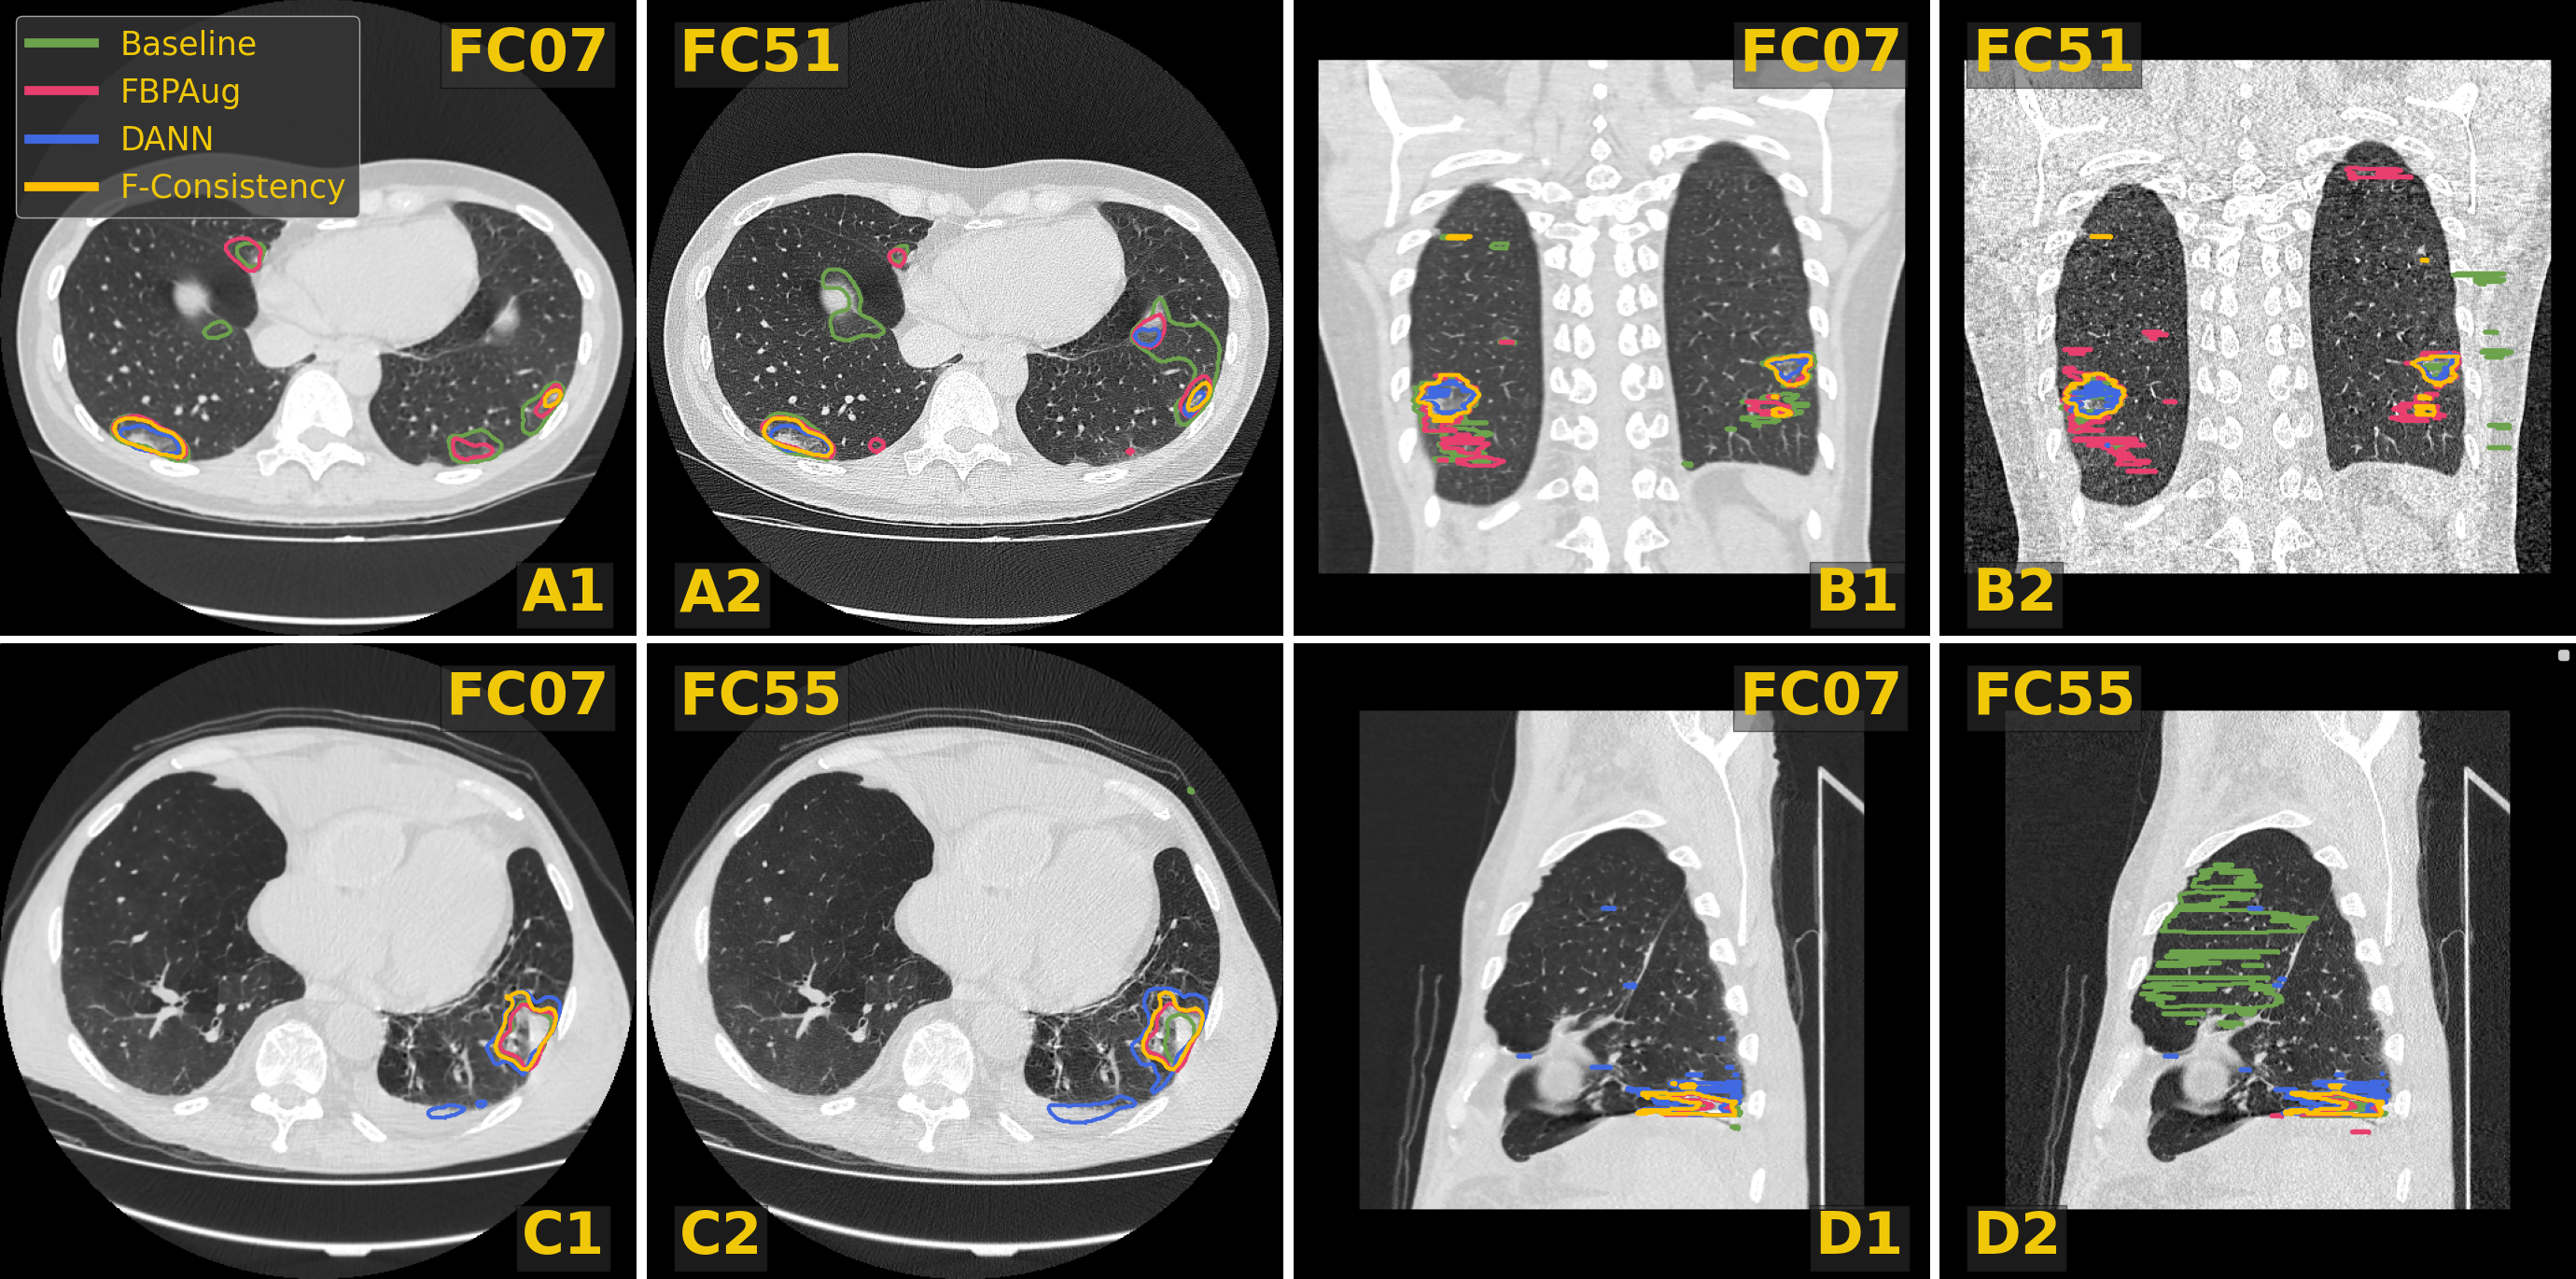
\includegraphics[width=\linewidth]{Dissertation/Figures/3_ct/consistency_preds.png}
	\caption{Examples of CT slices from the Private-paired dataset with the corresponding predictions on the paired images. Four doublets, denoted \textbf{A}, \textbf{B}, \textbf{C}, and \textbf{D}, contain corresponding slices from the smooth and sharp images. The doublets B and D are coronal and sagittal slices, respectively.}
	\label{fig:consistency_preds}
\end{figure}
\end{landscape}

%Below, we investigate the generalization of the models trained with fewer data and the trade-off between consistency and segmentation quality.


\textbf{Generalization with the less paired data.} We evaluate the models regularized using paired images from the Paired-public dataset. The dataset contains only FC07/FC51 and FC07/FC55 kernel pairs. Besides the previous setup, this data does not contain COVID-19 lesions. Thus, we show that some methods depend on the semantic content and poorly generalize to kernel styles. The results are shown in Table~\ref{tab:res_public}.



%\begin{table}[H]
%	\caption{Comparison of all adaptation methods from Table \ref{tab:res_final} except FBPAug trained on the Public-paired dataset. All results are Dice Scores in the format \textit{mean} $\pm$ \textit{std} calculated from $5$-fold cross-validation. We highlight the consistency scores near or below Baseline level in \textit{italic}. The best consistency scores are highlighted in \textbf{bold}.}
%	%\vspace{.2cm}
%	\begin{adjustwidth}{-\extralength}{0cm}
%		\newcolumntype{C}{>{\centering\arraybackslash}X}
%		\begin{tabularx}{\fulllength}{lCCCCCCC}
%			\toprule
%			
%			& \multirow{2.5}{*}{\shortstack{\textbf{COVID-Train}}} & \multirow{2.5}{*}{\textbf{COVID-Test}}& \multicolumn{5}{c}{\textbf{Paired-Private} \textbf{Consistency}} \\
%			\cmidrule(lr){4-8}
%			&  & & \textbf{FC07/55} & \textbf{FC07/51} & \textbf{LUNG/SOFT }& \textbf{LUNG/STAND }  & \textbf{Mean}\\
%			
%			\midrule
%			Baseline & $\mathbf{0.60 \pm 0.04}$ & $0.56 \pm 0.03$ & $0.52 \pm 0.06$ & $0.39 \pm 0.07$ & $0.58 \pm 0.08$ & $0.28 \pm 0.05$ & $0.46 \pm 0.05$\\
%			
%			% \cmidrule{1-8}
%			
%			% DANN (Dec) & $0.58 \pm 0.04$ & $0.63 \pm 0.04$ & $.62 \pm 0.03$ & $.49 \pm 0.07$ & $\mathit{.60 \pm 0.03}$ & $\mathit{.30 \pm 0.04}$ & $\mathit{.53 \pm 0.03}$ \\
%			
%			\cmidrule{1-8}
%			
%			% DANN & $.58 \pm 0.05$ & $.64 \pm 0.02$ & $.84 \pm 0.02$ & $.70 \pm 0.02$ & $.86 \pm 0.03$ & $.66 \pm 0.06$ & $.78 \pm 0.02$ \\
%			
%			% \cmidrule{1-8}
%			
%			DANN &  $\mathbf{0.60 \pm 0.03}$ &  $\mathbf{0.64 \pm 0.02}$ & $0.75 \pm 0.02$ & $\mathbf{0.64 \pm 0.05}$ & $0.67 \pm 0.03$ & $0.50 \pm 0.05$  & $0.66 \pm 0.02$ \\
%			
%			\cmidrule{1-8}
%			
%			% P-Cons & $0.59 \pm 0.04$ & $0.61 \pm 0.01$ & $0.65 \pm 0.05$ & $0.60 \pm 0.02$ & $0.77 \pm 0.01$ & $0.47 \pm 0.04$ & $0.63 \pm 0.03$\\
%			
%			% \cmidrule{1-8}
%			
%			P-Cons & $0.53 \pm 0.03$ & $0.58 \pm 0.03$ & $\mathit{0.54 \pm 0.05}$ & $\mathit{0.44 \pm 0.03}$ & $\mathit{0.57 \pm 0.04}$  & $\mathit{0.28 \pm 0.06}$ & $\mathit{0.47 \pm 0.03}$  \\
%			
%			\cmidrule{1-8}
%			
%			% F-Cons (Dec) & $0.60 \pm 0.03$ & $0.59 \pm 0.00$ & $\mathit{.54 \pm 0.05}$ & $\mathit{.47 \pm 0.05}$ & $\mathit{.64 \pm 0.05}$ & $\mathit{.31 \pm 0.06}$ &  $\mathit{.50 \pm 0.04}$ \\
%			
%			% \cmidrule{1-8}
%			
%			% F-Cons &  $0.57 \pm 0.03$ & $0.64 \pm 0.03$ & $0.88 \pm 0.01$ & $0.72 \pm 0.04$ & $0.83 \pm 0.02$ & $0.70 \pm 0.05$ & $0.80 \pm 0.01$ \\
%			
%			% \cmidrule{1-8}
%			
%			F-Cons & $0.59 \pm 0.04$ & $\mathbf{0.64 \pm 0.02}$ & $\mathbf{0.80 \pm 0.02}$ & $\mathbf{0.63 \pm 0.04}$ & $\mathbf{0.71 \pm 0.02}$ & $\mathbf{0.55 \pm 0.05}$ & $\mathbf{0.70 \pm 0.02}$  \\
%			
%			\bottomrule
%		\end{tabularx}
%		\label{tab:res_public}
%	\end{adjustwidth}
%\end{table}


\begin{table}[h]
	\centering
	\caption{Comparison of adaptation methods trained on the Public-paired dataset. All results are Dice scores in the format \textit{mean (std)} calculated from $5$-fold cross-validation.}
	%\vspace{.2cm}
	%\resizebox{\textwidth}{!}{%
		\begin{tabular}{lcccccc}
			\toprule
			& \multirow{2.5}{*}{\shortstack{COVID-\\test}} & \multicolumn{5}{c}{Paired-private consistency} \\
			\cmidrule(lr){3-7}
			& & FC07/55 & FC07/51 & soft/lung & stnd/lung & mean \\
			\midrule
			
			Baseline & 0.56(0.03) & 0.52(0.06) & 0.39(0.07) & 0.58(0.08) & 0.28(0.05) & 0.46(0.05) \\
			
			\cmidrule{1-7}
			
			P-Cons & 0.58(0.03) & 0.54(0.05) & 0.44(0.03) & 0.57(0.04) & 0.28(0.06) & 0.47(0.03) \\
			
			\cmidrule{1-7}
			
			DANN & \textbf{0.64(0.02)} & 0.75(0.02) & \textbf{0.64(0.05)} & 0.67(0.03) & 0.50(0.05) & 0.66(0.02) \\
			
			\cmidrule{1-7}
			
			F-Cons & \textbf{0.64(0.02)} & \textbf{0.80(0.02)} & 0.63(0.04) & \textbf{0.71(0.02)} & \textbf{0.55(0.05)} & \textbf{0.70(0.02)} \\
			
			\bottomrule
		\end{tabular}%}
		\label{tab:res_public}
\end{table}

We highlight two main findings from these results. Firstly, consistency of the method that operates with the decoder layers decreases to the level of Baseline; see P-Consistency in Table~\ref{tab:res_public}. Our intuition here is that the decoder version of the model can be more easily enforced to output the trivial predictions than the encoder one. Simultaneously, the images without COVID-19 lesions induce trivial predictions. Therefore, it might be easier for these models to differ the paired dataset from the source dataset by the semantic content and fail to align the stylistic features.

Finally, we observe our method, F-Consistency, to outperform the other adaptation methods training only on the publicly available data. At this point, FBPAug (Table~\ref{tab:res_final}) outperforms the adaptation methods. The latter indicates that the range of synthetically augmented data overlaps the range of Paired-public. So, if we have a large and representative set of paired data, enforcing consistency, as proposed F-consistency does, provides the best adaptation results. On the other hand, we can use the proposed augmentation method, FBPAug, in a zero-shot adaptation regime to achieve competitive performance if enough paired data is not provided.


\section{Summary}

We have proposed a new knowledge-driven augmentation method, FBPAug, to eliminate CT domain shifts related to the usage of different reconstruction kernels. It outperforms existing augmentation approaches and, in a zero-shot regime, other adaptation approaches. We also release the code, so FBPAug can be easily incorporated into any existing deep learning pipeline to ensure zero-shot domain adaptation in CT images.

Secondly, we have proposed an unsupervised domain adaptation method, F-Consistency, to address the same domain shift in CT reconstruction kernels. Our method uses a set of unlabeled CT image pairs and enforces the similarity between feature maps of paired images. We have shown that F-Consistency outperformed the other adaptation methods and FBPAug in the COVID-19 segmentation task \textit{when provided with enough unlabeled data}. Finally, through extensive evaluation, we have shown our method to generalize to the unseen reconstruction kernels better and without the specific semantic content.



	

%\chapter{Benchmark for DA in 3D Medical Image Segmentation}
\chapter{Systematically Evaluating DA Methods in 3D Medical Image Segmentation}
\label{chap:da_bench}


Domain shift presents a significant challenge in applying Deep Learning to the segmentation of 3D medical images from sources like Magnetic Resonance Imaging (MRI) and Computed Tomography (CT). Although numerous Domain Adaptation methods have been developed to address this issue, they are often evaluated under impractical data shift scenarios. Specifically, the medical imaging datasets used are often either private, too small for robust training and evaluation, or limited to single or synthetic tasks.

To overcome these limitations, we first introduce a M3DA benchmark comprising four publicly available, multiclass segmentation datasets. We have designed eight domain pairs featuring diverse and practically relevant distribution shifts. These include inter-modality shifts between MRI and CT and intra-modality shifts among various MRI acquisition parameters, different CT radiation doses, and presence or absence of contrast enhancement in images.

Within the proposed benchmark, we evaluate more than ten existing domain adaptation methods. Our results show that none of them can consistently close the performance gap between the domains. For instance, the most effective method reduces the performance gap by about 62\% across the tasks. This highlights the need for developing novel domain adaptation algorithms to enhance the robustness and scalability of deep learning models in medical imaging.

Secondly, we collect and publish the Burdenko's Glioblastoma Progression (BGP) dataset, a systematic and annotated data collection of glioblastoma MRI scans from multiple clinical sites, acquired using scanners from four different vendors and varying imaging protocols. This dataset provides a clinically relevant ``in-the-wild'' domain adaptation setup, where models must generalize across real-world acquisition variability. By including this dataset, we bridge the gap between methodological advancements in domain adaptation research and its practical deployment in clinical settings.


\section{Introduction}

Deep Learning (DL) methods have significantly advanced medical image analysis, achieving near-human-level performance in tasks like image classification, segmentation, pathology detection, and automated diagnosis \cite{medim_dl_survey_2017}. However, the widespread adoption of DL in medical imaging is hindered by the poor performance of neural networks on data from distributions different from their training set. This challenge, known as \textbf{domain shift}, is particularly prevalent in medical imaging due to changes in scanner acquisition parameters, the introduction of new imaging modalities, and population differences. Several studies have concluded that medical imaging is a crucial domain for the adoption of Domain Adaptation (DA) methods \cite{gulrajani2020search,uda_survey_2020,zhuang2020comprehensive,peng2018visda,zhang2021empirical}. Despite this, there is a lack of a common benchmark for testing DL methods in the field of 3D medical imaging.


\begin{figure*}[h]
	\centering
	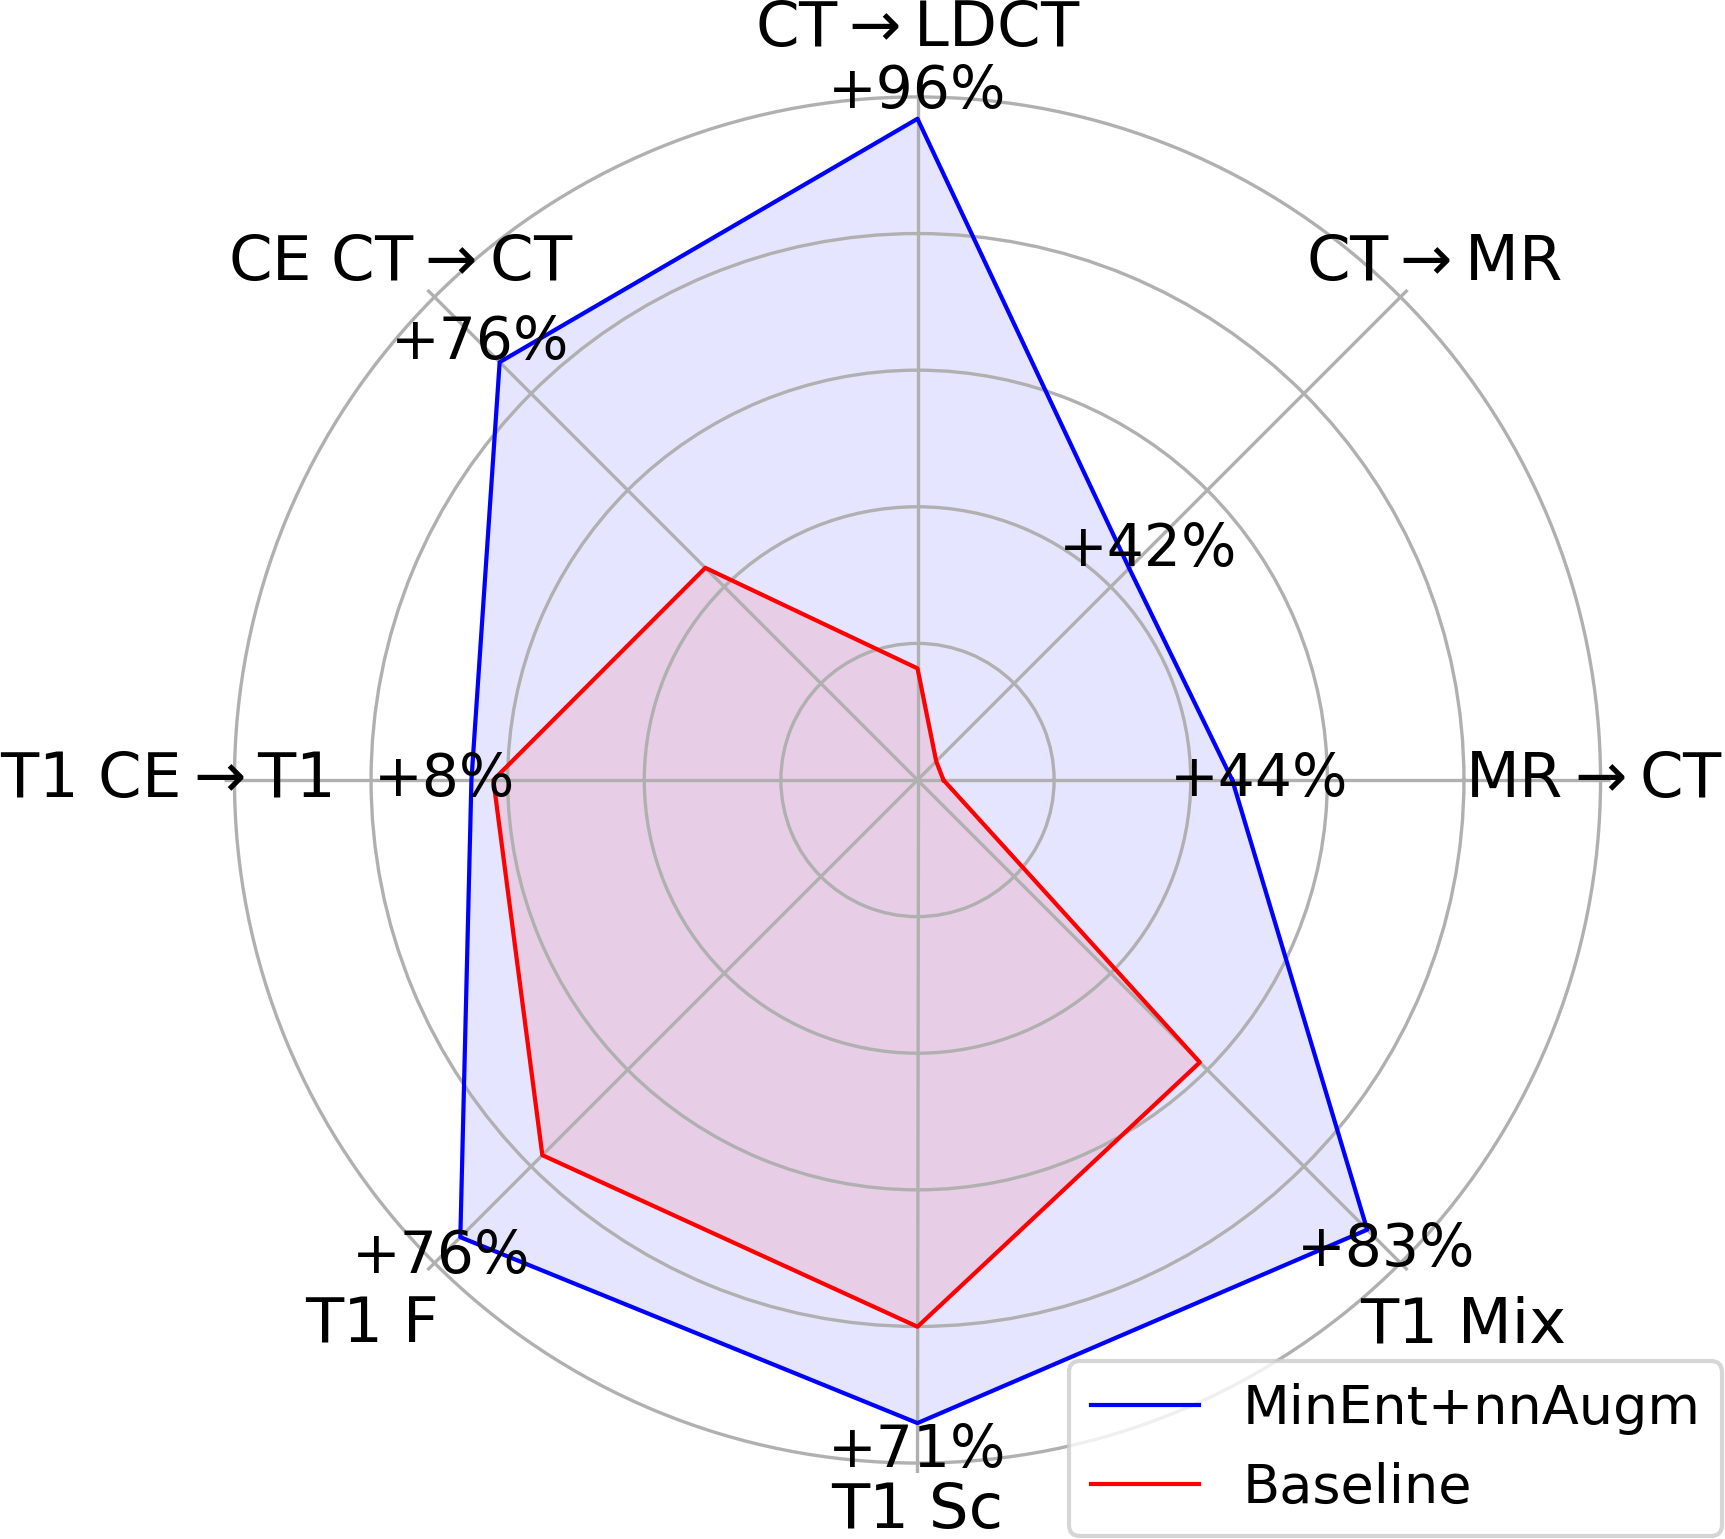
\includegraphics[width=0.80\linewidth]{Dissertation/Figures/4_da_bench/fig1_teaser.png}
	\caption{Using the best DA method in the M3DA benchmark closes only 62\% of the performance gap between domains on average. Here, \% indicates the gap closed between the baseline level and oracle (outer) circle.}
	\label{fig:teaser1}
\end{figure*}


\begin{figure*}[h]
	\centering
	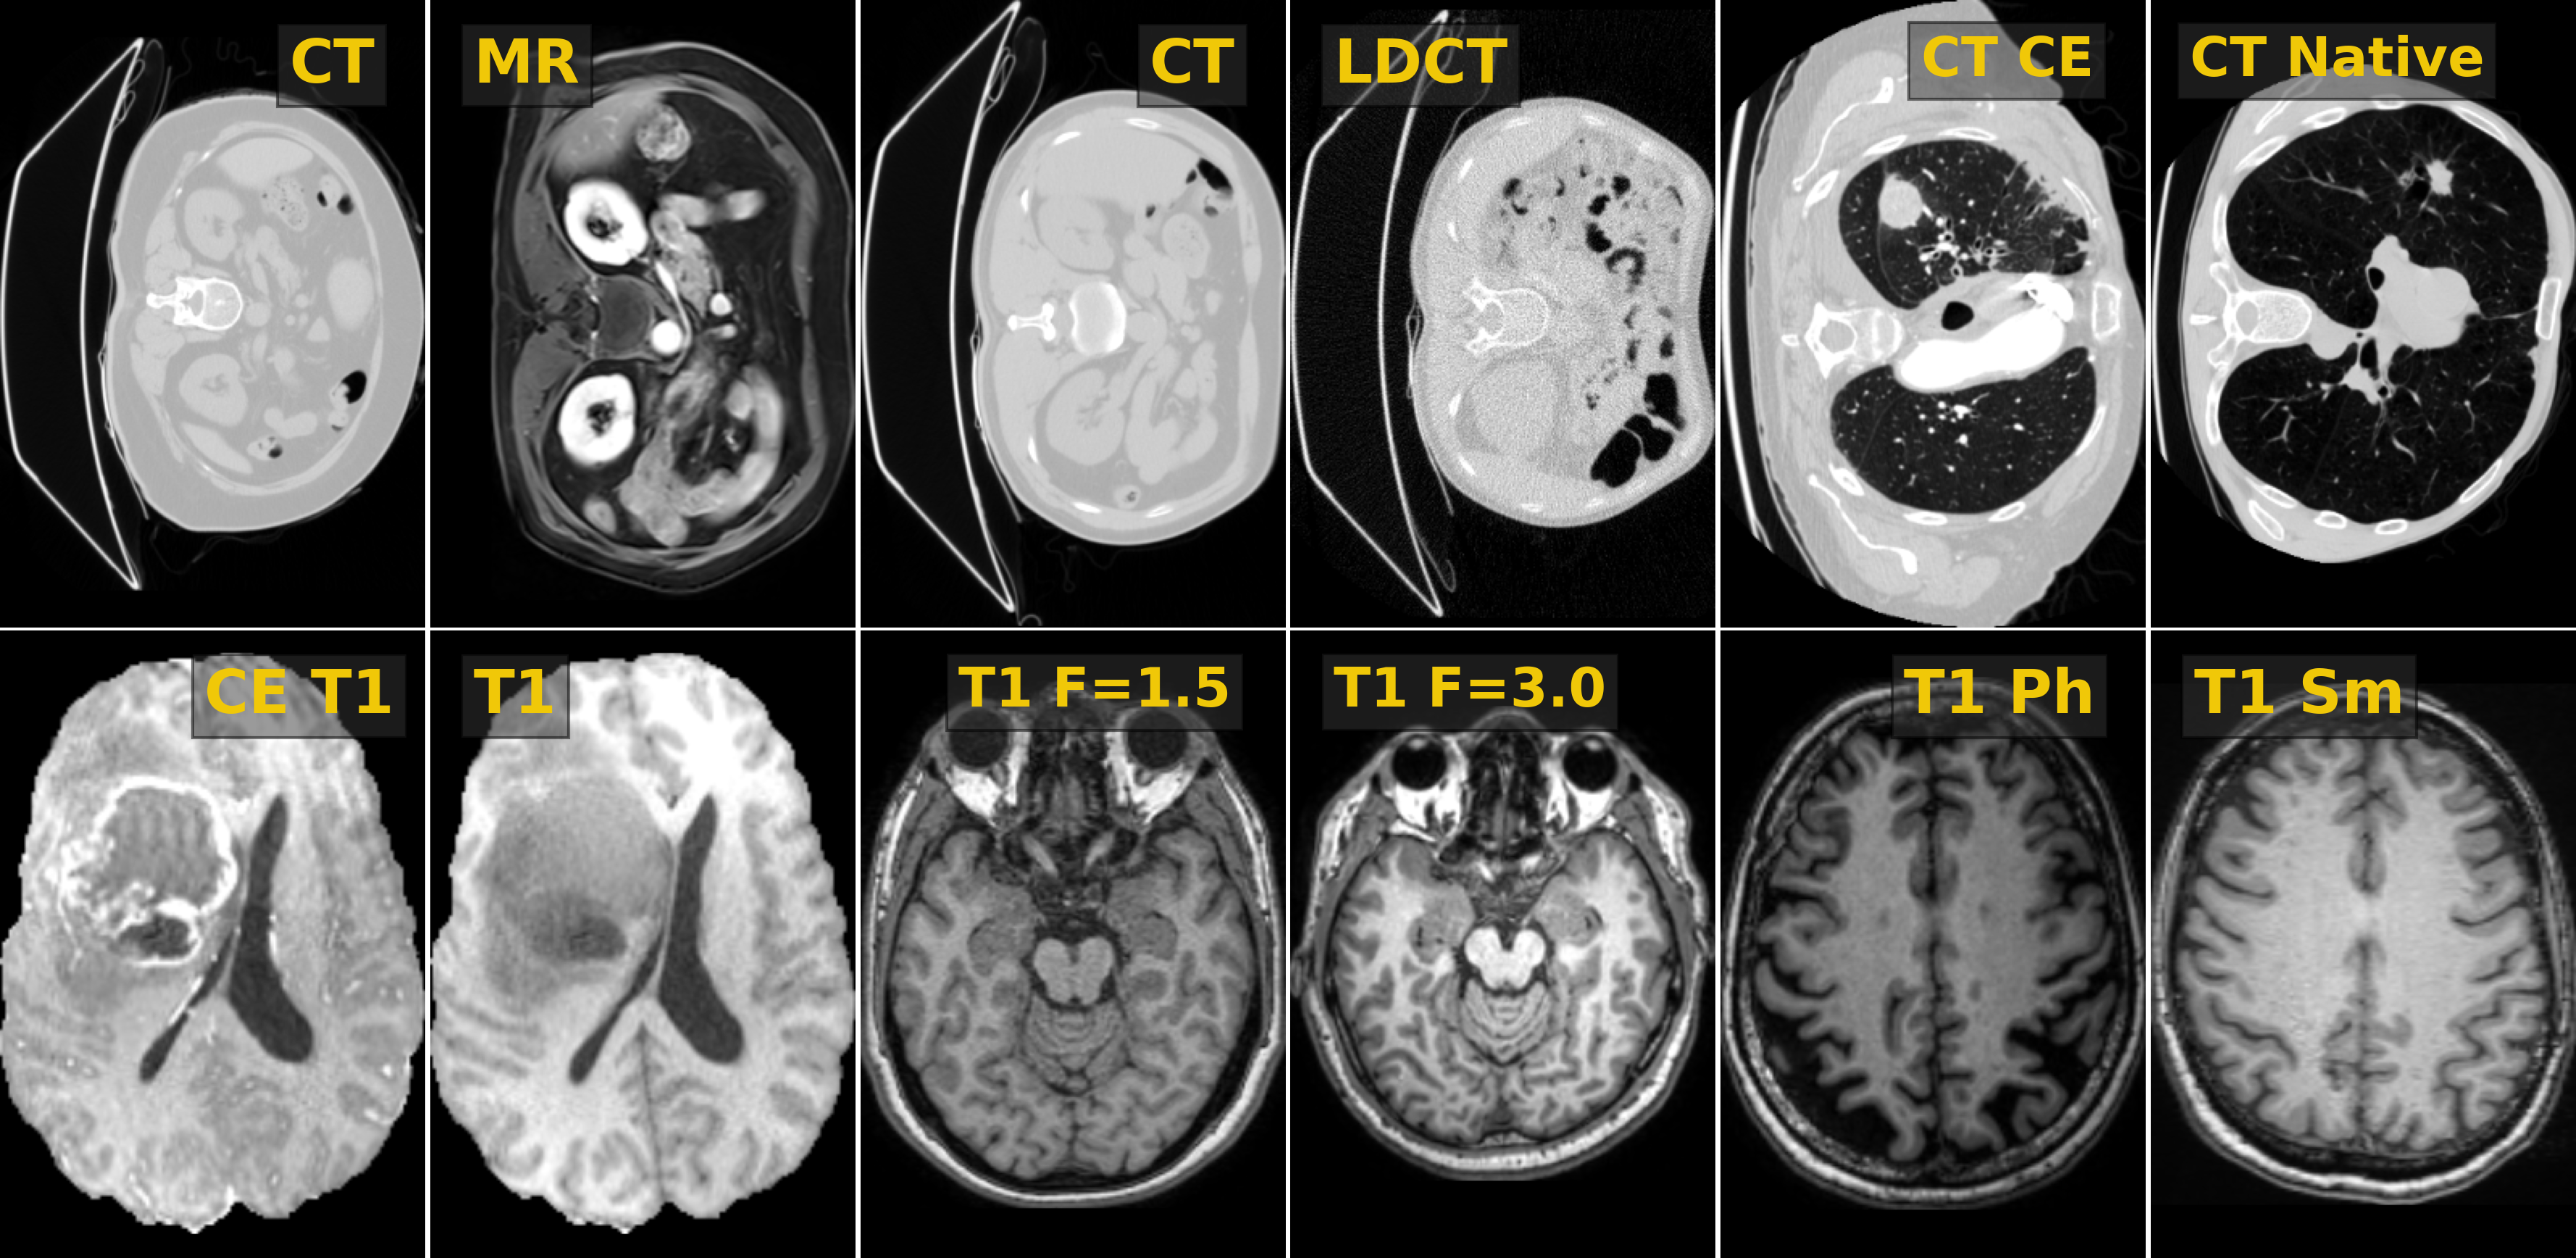
\includegraphics[width=1\linewidth]{Dissertation/Figures/4_da_bench/fig2_bench_examples.png}
	\caption{Examples from individual domains in M3DA without segmentation masks for visual comparison between domains. Left to right, top to bottom: CT to MR, CT to LDCT, CT CE to CT native, CE T1 to T1, T1 Field (1.5T to 3T), T1 Scanner (Philips to Siemens).}
	\label{fig:teaser2}
\end{figure*}


\begin{figure*}[h]
	\centering
	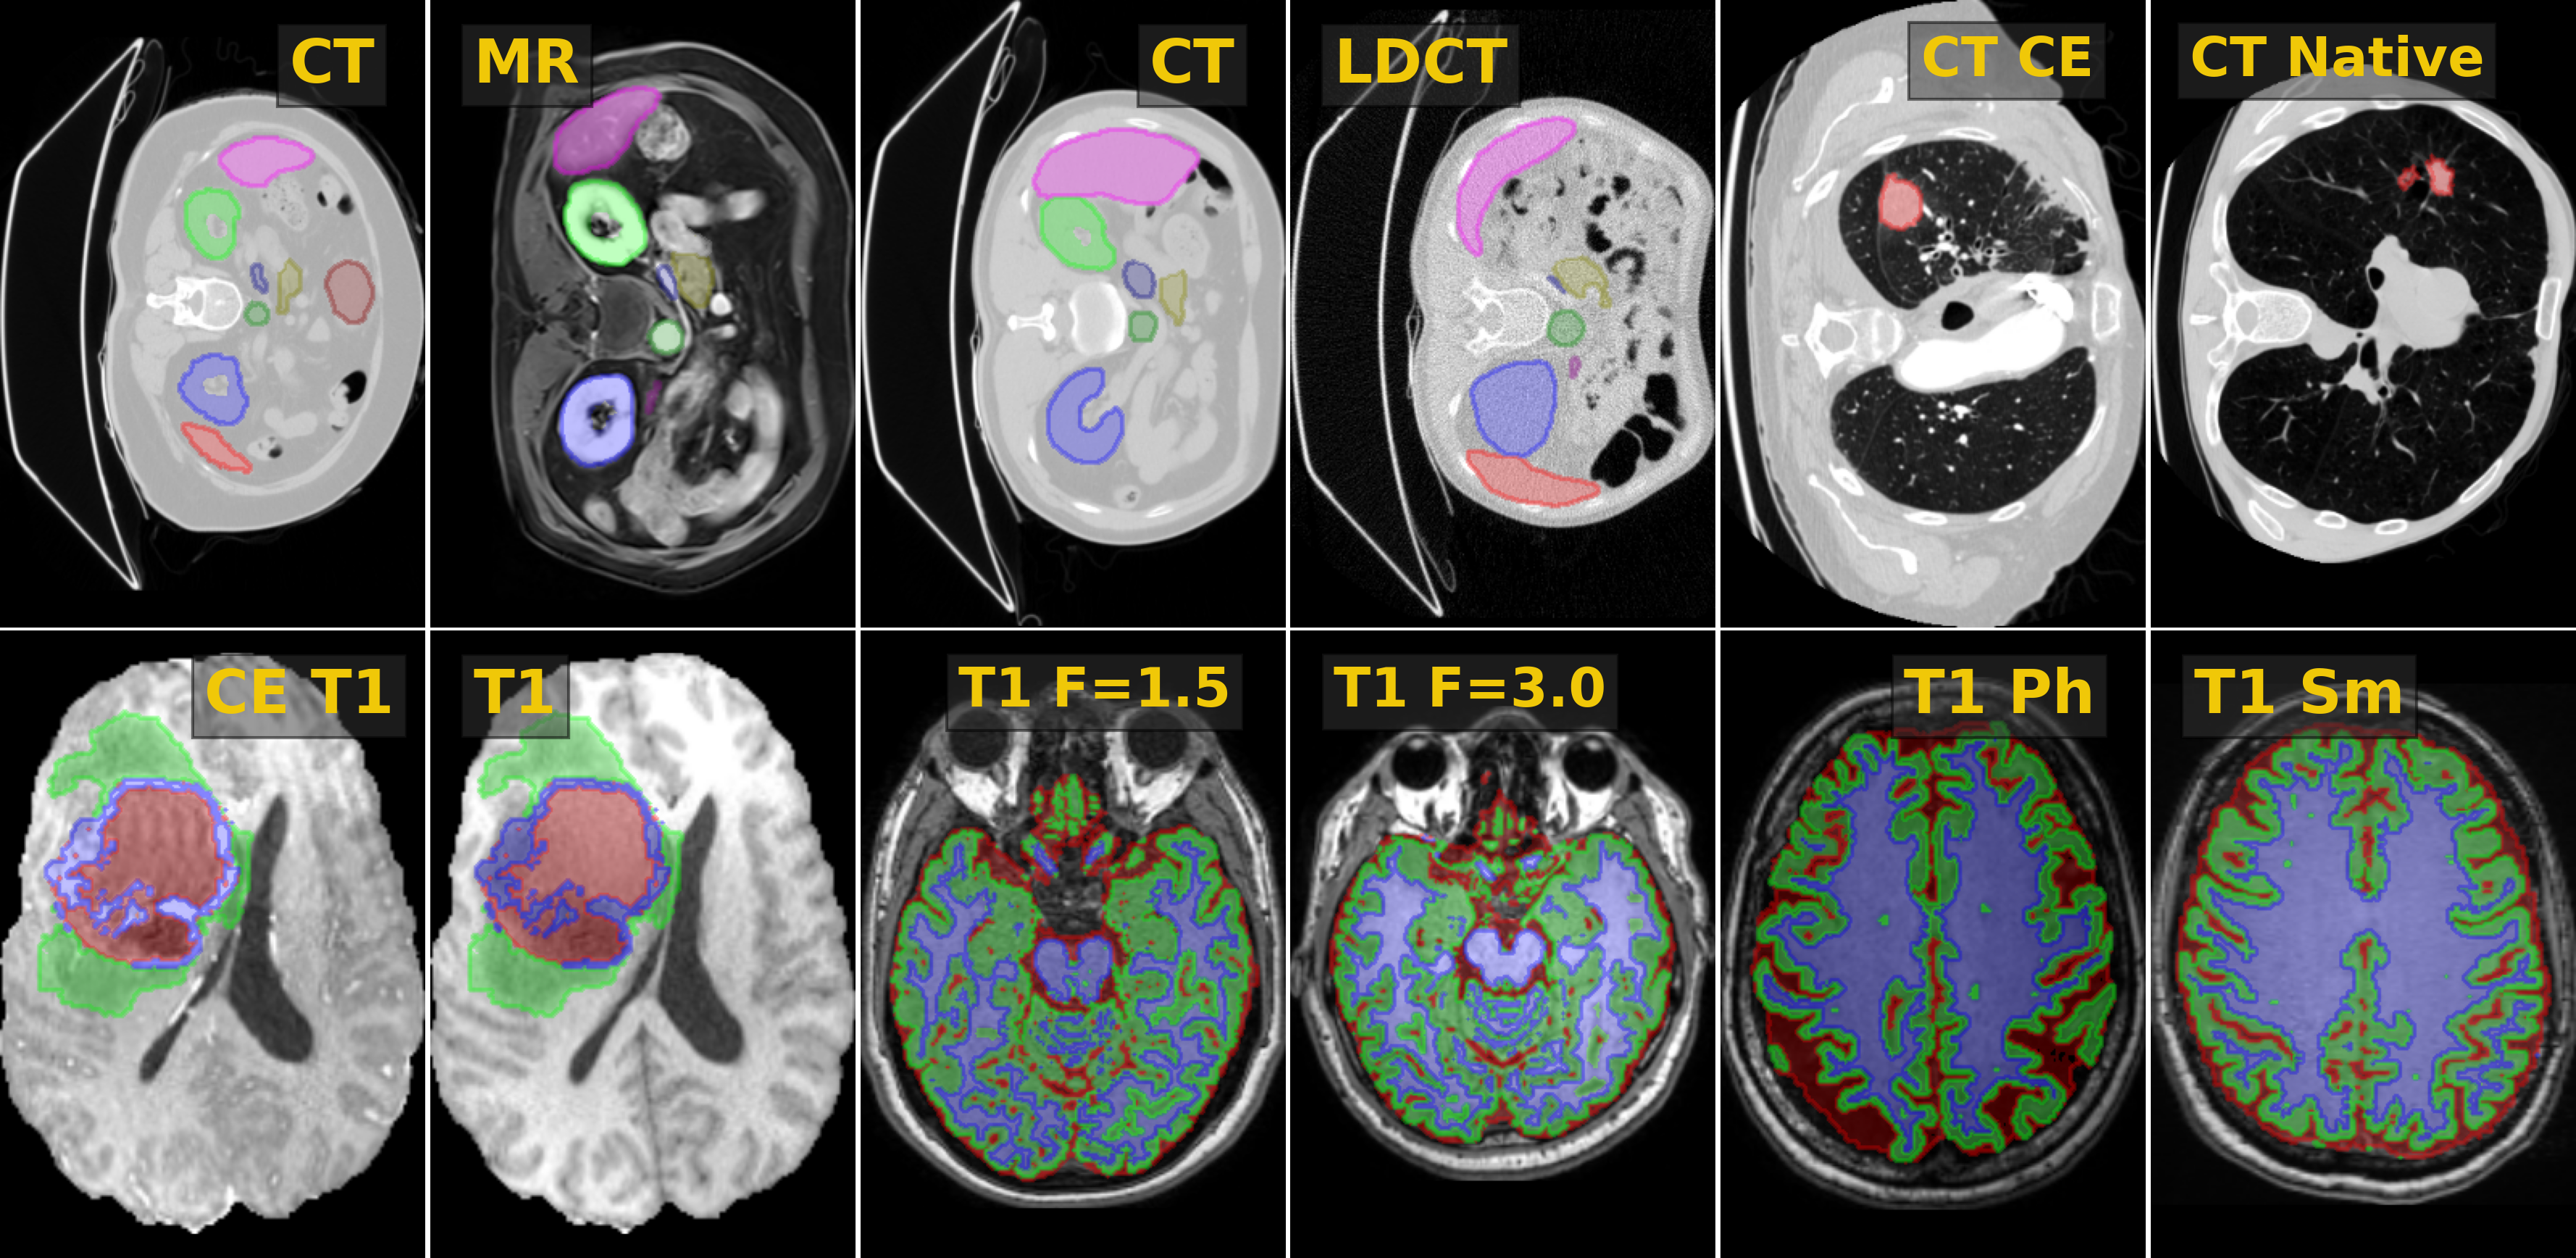
\includegraphics[width=1\linewidth]{Dissertation/Figures/4_da_bench/fig2_bench_contours.png}
	\caption{Examples from individual domains in M3DA with the corresponding segmentation masks. Left to right, top to bottom: CT to MR, CT to LDCT, CT CE to CT native, CE T1 to T1, T1 Field (1.5T to 3T), T1 Scanner (Philips to Siemens). Different colors correspond to different segmentation classes.}
	\label{fig:contours}
\end{figure*}

Recent works have focused on developing DA methods, revealing that 3D medical image segmentation algorithms are particularly susceptible to domain shift. Researchers have tested their methods against various sources of domain shift, including shifts between imaging modalities, the most common being MRI and CT \cite{jiang2020unified,yu2023source,zheng2021hierarchical}. Other sources of domain shift include scanner manufacturers or settings, such as the strength of MR field or CT dosage \cite{zheng2021hierarchical,liu2020shape,chen2022maxstyle,gu2021domain,lennartz2023segmentation,se_medim}, and intra-modality shifts, such as T2 to T1 MRI \cite{han2021deep,crossmoda,dann_medim}.

A systematic comparison of these methods, along with the question of the necessity to develop new ones, is complicated by lack of consistency in the usage of datasets across studies, even when addressing similar domain shifts, as shown in Table~\ref{tab:benchmarks}. In addition, many studies test their proposals on a single domain shift problem, limiting the generalizability of their analysis.  

Recently, the Cross-Modality Domain Adaptation (CrossMoDA) challenge \cite{crossmoda}, conducted at MICCAI in 2021 and repeated in 2022 and 2023, attempted to unify various authors under the same framework. The challenge's setup involved training models on annotated MR T1c with access to unannotated T2 studies, followed by testing on T2 studies. The challenge attracted numerous participants, with the top teams achieving near-supervised performance levels using image-to-image translation techniques paired with multi-stage pseudo-labeling.

Despite its success, the CrossMoDA challenge has certain limitations. Firstly, it only considers a single source of domain shift, the MR sequence. Secondly, the segmentation task is confined to a two-class challenge: segmenting the vestibular schwannoma tumor and the cochlea, both located in very specific anatomical regions. Consequently, top-performing solutions managed to close up to a 97\% score gap between domains. Participants employed various task-specific techniques, such as using only the largest connected component of the segmentation mask to enhance segmentation quality. While this approach may be effective for solving a concrete segmentation task, it is counterproductive for assessing the capabilities of DA methods. It obscures the true impact of adaptation to the unseen domain, hindering a clear understanding of the effectiveness of DA techniques.

\textit{Therefore, we conclude that there is a need for a large, diverse, and publicly available benchmark for DA in 3D medical image segmentation that includes a variety of downstream tasks.} We introduce such a benchmark to encourage further progress in developing scalable DA methods.

We include four publicly available datasets, encompassing 22 segmentation tasks. Based on these datasets, we construct eight domain adaptation problems; see visual examples of individual domains in Figure~\ref{fig:teaser2} with the corresponding segmentation masks in Figure~\ref{fig:contours}. Table~\ref{tab:setup} summarizes all proposed problems with their domain shifts and dataset splits.

To establish a baseline and determine which problems remain unsolved with current methods, we implemented core unsupervised DA (UDA) methods for 3D medical image segmentation. Excluding any task-specific assumptions (e.g., filtering the largest connected component) and human-in-the-loop approaches, the best method within our benchmark closes only 62\% of the performance drop between domains on average. Thus, we highlight the need for further development of robust DA methods in 3D medical image segmentation, with our proposed benchmark serving as a strong foundational point for systematically comparing novel methods. We summarize our contributions as follows:

\begin{itemize}
	
	\item We propose a benchmark for DA in 3D medical image segmentation that includes eight carefully selected domain shifts based on their practical relevance. These shifts cover variations in imaging modalities, scanner settings, and the presence of contrast agents, ensuring that our benchmark reflects real-world challenges in medical image analysis.
	
	\item We provide a comprehensive evaluation of more than ten core domain adaptation methods on our benchmark, covering key categories of UDA approaches. 
	
	\item Our benchmark is designed to be economical, utilizing only four publicly available datasets. This allows for testing new methods against a wide variety of problems with minimal resources, making our benchmark accessible to researchers and encouraging wider adoption.
	
\end{itemize}


\section{M3DA Benchmark}
%\label{sec:bench}

We consider a semantic segmentation problem of 3D medical images, which we call a downstream task. Any downstream model works with input samples $x \in X$ and the corresponding segmentation masks $y \in Y$, where $X$ and $Y$ are some input image and label spaces. If $x \in \R^{H \times W \times D}$, segmentation mask is of the same spatial size $y \in \R^{H \times W \times D}$, where every element belongs to a predefined set of labels $y^{(h,w,d)} \in \{ 0, 1, \dots, C \}$, $0$ is background and $C$ is the number of foreground classes.



\begin{table}[ht]
	\centering
	\caption{Comparison to the existing benchmark (CrossMoDA) and datasets that are commonly used for Domain Adaptation in 3D medical image segmentation. Our proposed benchmark (M3DA) covers all primary domain shifts with the largest publicly available datasets.}
	
	\resizebox{\textwidth}{!}{%
		\begin{tabular}{lccccc}
			\toprule
			\textbf{Paper} & \textbf{Domain shifts} & \textbf{Datasets} & \textbf{Modalities} & \textbf{Region of interest} \\
			\midrule
			Jiang at al., 2020 \cite{jiang2020unified} & inter-modality & BTCV, CHAOS & MRI, CT &  4 thoracic organs  \\
			Al et al., 2021 \cite{al2021olva} & inter-modality & MM-WHS & MRI, CT & heart \\
			Weihsbach at al., 2024 \cite{dg_tta} & inter-modality & AMOS, MM-WHS,  spine & MRI, CT & 15 thoracic organs, brain, spine \\
			Liu et al., 2020 \cite{liu2020shape}             & MRI settings, scanners & 6 public datasets      & MRI              &  prostate         \\
			Gu et al., 2021 \cite{gu2021domain}             & MRI settings, scanners & SAML                   & MRI              &  prostate         \\
			Chen et al., 2022 \cite{chen2022maxstyle}         & MRI settings, scanners & ACDC, M\&Ms            & MRI              &  heart            \\
			Lennartz et al., 2023 \cite{lennartz2023segmentation} & MRI settings, scanners & CC359, ACDC, M\&Ms     & MRI              &  brain, heart     \\
			Wong et al., 2023 \cite{wong2023hartleymha}       & MRI settings, scanners & BraTS                  & MRI              &  brain            \\
			Liu et al., 2022 \cite{liu2022act}               & MRI inter-sequence & BraTS                  & MRI              &  brain            \\
			CrossMoDA, 2023 \cite{crossmoda}                & MRI inter-sequence & Vestibular Schwannoma  & MRI              &  brain            \\
			
			\midrule
			
			\multirow{2}{*}{M3DA (ours)} & inter-modality, inter-sequence & \multirow{2}{*}{AMOS, CC359, BraTS, LIDC} & \multirow{2}{*}{MRI, CT} & brain, tumors, \\
			& CT/MRI settings, scanners, contrast & & & 15 thoracic organs \\
			
			\bottomrule
	\end{tabular}}
	
	\label{tab:benchmarks}
\end{table}



We follow the standard unsupervised domain adaptation (UDA) problem setting, as in \cite{dann}. We assume that two distributions $\mathcal{S}(x, y)$ and $\mathcal{T}(x, y)$ exist on $X \otimes Y$, called \textit{source} and \textit{target} distributions. At the training time, we have a set of source training samples $X^s = \{ x_i^s \}_{i=1}^n$ with the corresponding masks $Y^s = \{ y_i^s \}_{i=1}^n$ and a set of target training samples $X^t_{tr}$ without annotations; source images and masks are considered to be sampled from $\mathcal{S}$, $(x_i^s, y_i^s) \sim \mathcal{S}(x, y)$. Our goal is to predict segmentations $y$ given the input from the marginal distribution of target images, $x \sim \mathcal{T}(x)$. To evaluate algorithms, we have target testing samples $X^t_{ts}$ with masks $Y^t_{ts}$ \textit{available only for evaluation purposes}.

Thus, given domains A and B, one trains a supervised model on domain A while having access to unannotated samples from domain B for adaptation. The goal of UDA is to develop a model that makes accurate predictions on domain B. Importantly, this setup prohibits incorporating annotations from the target domain into the training routine.



\subsection{UDA Problems Motivation}
%\label{ssec:constructing}




\begin{table}[h]
	\centering
	\caption{Summary of the datasets commonly used in DA studies. ROI stands for region of interest, and \#cls denotes the number of foreground segmentation classes. Several datasets do not contain inner domain shifts, i.e., \textit{single source}; they are used in multi-dataset setups.}
	
%	\resizebox{\linewidth}{!}{%
		\begin{tabular}{@{}lcccc@{}}
			\toprule
			\textbf{Dataset} & \textbf{Modality} & \textbf{ROI} & \textbf{\#cls} & \textbf{\#cases} \\
			\midrule
			WMH \cite{wmh} & MRI & Brain & 2 & 60 \\
			BraTS \cite{brats} & MRI & Brain & 3 & 1251 \\
			CC359 \cite{cc359} & MRI & Brain & 5 & 359 \\
			ACDC \cite{bernard2018deep} & MRI & Heart & 2 & 150 \\
			M\&Ms \cite{campello2021multi} & MRI & Heart & 6 & 375 \\
			SCGM \cite{prados2017spinal} & MRI & Spinal Cord & 2 & 80 \\
			IVDM3Seg \cite{IVDM3Seg2018} & MRI & Spinal Cord & 2 & 16 \\
			BTCV \cite{btcv} & CT & Abdomen & 13 & 30 \\
			AMOS \cite{amos} & CT, MRI & Abdomen & 15 & 500, 100 \\
			CHAOS \cite{kavur2021chaos} & CT, MRI & Thorax & 4 & 50 \\
			MM-WHS \cite{zhuang2016multi} & CT, MRI & Heart & 8 & 20, 20 \\
			\bottomrule
	\end{tabular}%}
	\label{tab:datasets}
\end{table}



\paragraph{CT \textbf{$\leftrightarrow$} MRI}

First, we include domain shift from MRI to CT and vice versa. Although the use of CT scans is often clinically justified, it is associated with additional risks, such as 
potentially increasing the risk of cancer \cite{cao2022ct,brenner2007computed}. In contrast, MRI is a safer imaging modality that does not involve radiation exposure \cite{nie2016estimating}. While CT is critical for various clinical applications like radiotherapy treatment planning, there is a recent transition to MRI for these applications \cite{paczona2023magnetic}. Thus, developing algorithms that use decades of collected CT data and adapt them for newly acquired MRI scans is an important avenue of research.

The inverse problem of estimating MRI from CT is also an important application. CT is a much faster imaging modality compared to MRI, making it a better solution in emergency scenarios such as stroke. However, MRI provides more sensitive brain visualization \cite{vymazal2012comparison}. Therefore, having universal algorithms that can adapt to the needed modality at hand is highly beneficial.

While these examples highlight the clinical relevance of domain adaptation between CT and MRI, for the purpose of this benchmark, we utilize a different dataset focusing on thoracic organ segmentation. This choice is motivated by the availability of a dataset that provides both MR and CT images with corresponding segmentation maps for thoracic organs, which is essential for evaluating the performance of UDA algorithms. Despite the difference in the target application, the underlying principles of domain adaptation remain the same, and the insights gained from this benchmark can be applied to various clinical scenarios.


\paragraph{CT $\rightarrow$ low-dose CT}

Second, we include a CT to low-dose CT (LDCT) shift, motivated by the increasing popularity of LDCT. LDCT produces images with a lower signal-to-noise ratio but are still diagnostically effective, resulting in several-fold lower radiation dosage exposure compared to regular CT (allowing for screening purposes \cite{lidc,kubo2016standard}), faster scanning time, mobility to scan underserved populations \cite{raghavan2020initial}, and cost-effectiveness \cite{mohammadshahi2019cost}. Similar to the CT $\leftrightarrow$ MRI domain shift, utilizing publicly available annotated regular CT scans can accelerate the development of automated segmentation models for LDCT. As demonstrated in Table~\ref{tab:metrics_pure}, methods trained on regular CT perform poorly on LDCT. This shift is the only one obtained via simulation, where we algorithmically simulate low-dose CT from regular ones.


\paragraph{Contrast enhancement $\rightarrow$ no contrast enhancement}

Third, we include two tasks, MRI and CT, involving domain transfer from a contrast-enhanced (CE) image to an image without contrast enhancement (native). CE injection is a labor-intensive step, requiring additional training for personnel and carrying a small but additional risk for patients \cite{andreucci2014side,costelloe2020risks}. Again, we suggest benchmarking DA methods against the scenario where models that utilized richer imaging modalities (CE) during supervised training are adapted for safer modalities (non-contrast-enhanced).


\paragraph{MRI settings}

Finally, we include three setups that address the domain shifts caused by variable MRI scanner settings, which are among the most common sources of domain shift encountered in practice \cite{yan2020mri,medim_da_survey_2023}. These setups cover different field strengths (1.5T vs. 3T), different scanner manufacturers, and a combination of both. Domain shifts arising from variations in scanner settings are ubiquitous in multi-source MRI datasets, as differences in field strength and manufacturer-specific acquisition parameters can significantly impact the appearance and quality of the resulting images. Addressing these shifts is crucial for developing robust and generalizable segmentation models that can handle the heterogeneity of MRI data encountered in real-world clinical scenarios.



\subsection{Datasets selection}
%\label{ssec:data}

We base the inclusion of datasets into the benchmark on two criteria. \textbf{Relevance}, we aim to cover as many relevant domain shifts as possible; see Section~\ref{sec:da_bench:exp:limitations} for a list of domain shifts not included in our benchmark. \textbf{Scale}, we prefer a dataset with a larger number of samples, when deciding between two datasets that are both relevant and include similar domain shifts. All reviewed and selected datasets are summarized in Table~\ref{tab:datasets}, and all technical details (e.g., links, download instructions, and licenses) are provided in Appendix~\ref{app:m3da_datasets}.



\begin{table}[h]
	\centering
	\caption{Details of eight tasks in M3DA benchmark. The last three columns correspond to the numbers of cases in \textit{source}, \textit{target train}, and \textit{target test} folds, respectively.}
	
%	\resizebox{\linewidth}{!}{%
		\begin{tabular}{@{}lccccc@{}}
			\toprule
			\textbf{Task name} & \textbf{Domain shift} & \textbf{Dataset} & $|X^s|$ & $|X^t_{tr}|$ & $|X^t_{ts}|$ \\
			\midrule
			MR$\ra$CT & inter-modality & AMOS & 60 & 200 & 150 \\
			CT$\ra$MR & inter-modality & AMOS & 150 & 40 & 60 \\
			CT$\ra$LDCT & CT settings & AMOS & 150 & 200 & 150 \\
			CE CT $\ra$ CT & settings (contrast) & LIDC & 289 & 297 & 297 \\
			% T1$\ra$T2 & intra-modality & BraTS & 625 & 313 & 313 \\
			% T2$\ra$T1 & intra-modality & BraTS & 625 & 313 & 313 \\
			% T1$\ra$T1c & settings (contrast) & BraTS & 625 & 313 & 313 \\
			T1 CE$\ra$T1 & settings (contrast) & BraTS & 625 & 313 & 313 \\
			T1 F & MRI settings & CC359 & 30 & 30 & 30 \\
			% T1 Sc & MRI scanners & CC359 & 30 & 20 & 21 \\  % add unlbl
			T1 Sc & MRI scanners & CC359 & 30 & 30 & 30 \\
			T1 Mix & settings, scanners & CC359 & 29 & 30 & 30 \\
			\bottomrule
	\end{tabular}%}
	
	\label{tab:setup}
\end{table}


We start by selecting a dataset for MRI to CT conversion. This allows for several alternatives. Many authors use datasets such as BTCV and CHAOS for these tasks, both of which include images of the thoracic region. BTCV consists of 30 CT scans with 13 organ annotations, and CHAOS of 40 MRI and 40 CT scans with 4 organ annotations. Another option is MM-WHS, which consists of 20 MRI and 20 CT scans of the heart with 8 annotated classes. Finally, there is the newer AMOS dataset, which consists of 500 CT and 100 MRI scans with 15 annotated thoracic organs. Following our criteria, we include AMOS as it is the largest option. We also use AMOS to simulate LDCT data.

To cover CE CT to native CT task, we add Lung Image Database Consortium image collection (LIDC) \cite{lidc}. LIDC contains chest CT images with and without contrast enhancement with segmentation annotation of lung nodules. LIDC dataset covers lung nodules - an oncology pathology, one of the most common reasons for using contrast enhancement \cite{purysko2016does}. Then, we cover the similar CE-based data shift in multi-sequence MRI data, from T1 CE to T1 modality. BraTS 2021, being one of the largest and most widely used datasets in the medical imaging community, emerges as the natural choice, satisfying our criteria of relevance, and scale.

Finally, we cover variability in the single-sequence MRI acquisition. As evident from Tables \ref{tab:benchmarks} and \ref{tab:datasets}, common choices are the ACDC and M\&Ms datasets. Both include segmentation classes of the heart and are relatively large, consisting of 150 and 375 annotated samples, respectively. Both have several concretely defined MRI domains (e.g., different scanners, parameters, field strengths). Another option is CC359, which has the same rich variability in MRI parameters and is similarly sized, including 359 annotated samples. Both ACDC and M\&Ms images have $1\times 1\times 9~ \text{mm}^3$ spacing, for which a 2D algorithm would often be a more viable choice. In contrast, a significant advantage of CC359 is the fine-grade and consistent voxel spacing, approximately $1\times 1\times 1~ \text{mm}^3$, which concludes our selection. UDA setups from the selected datasets are summarized in Table~\ref{tab:setup}.


\section{Methods for M3DA Benchmark}
\label{sec:methods}


\begin{figure}[!ht]
	\centering
	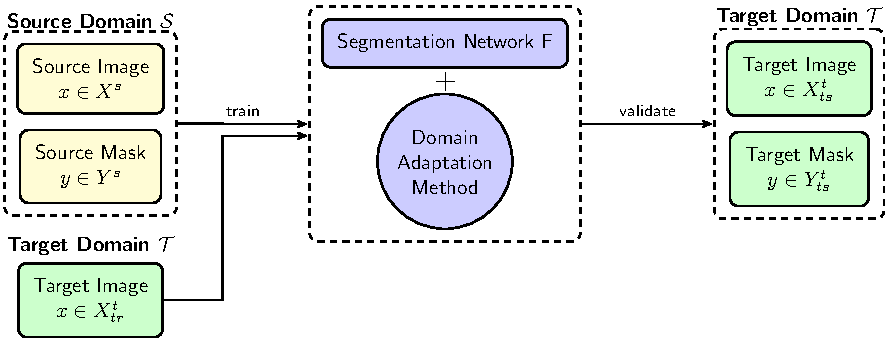
\includegraphics[width=1\columnwidth]{Dissertation/Figures/4_da_bench/uDA_pipeline.pdf}
	\caption{Overview of the UDA pipeline for semantic segmentation. Some methods does not require Target Domain images during training, e.g., nnAugm, IN, AdaBN.}
	\label{fig:pipeline}
\end{figure}

% Since our downstream task is semantic segmentation, a conventional way to solve it is training a convolutional neural network. In particular, U-Net \cite{unet} architecture and its variants are widely adopted in medical image segmentation. We also use an established version of U-Net as a baseline and describe it in Section~\ref{ssec:baseline}. The adaptation to target distribution can be performed in a variety of ways, e.g., transferring images styles between $X^s$ and $X^t_{tr}$ via CycleGAN \cite{cyclegan} or learning domain-invariant features via DANN \cite{dann}. We detail UDA methods included in our benchmark in Section~\ref{ssec:uda}.


\subsection{Segmentation baseline and oracle}
\label{ssec:baseline}

Let $F$ be a segmentation network which takes an image $x \in \R^{H \times W \times D}$ and predicts a soft-segmentation map $p = F(x)$, $p \in \R^{H \times W \times D \times (C + 1)}$. Here, the last layer of $F$ is softmax which outputs a $(C+1)$-dimensional voxel-wise vector $\left[p^{(h, w, d, c)}\right]_c$ behaving as a discrete distribution over classes. The parameters $\theta_F$ of $F$ are learned to minimize some segmentation loss $\mathcal{L}_{seg} (p, y)$. In our case, $\mathcal{L}_{seg}$ is a sum of cross-entropy and Dice losses, as used by default in \cite{nnunet} and many other works. Optimization problem for training on source domain reads:

\begin{equation}
	\min_{\theta_F} \frac{1}{|X^s|} \sum_{(x, y) \in (X^s, Y^s)} \mathcal{L}_{seg} (F(x), y).    
\end{equation}

Further, every DA method depends on $F$, i.e., has the same backbone, so the choice of $F$ is crucial for the benchmark construction. We used the nnU-Net \cite{nnunet} architecture, loss function, and training pipeline, since nnU-Net demonstrated the best performance in several relevant tasks \cite{nnunet,amos,isensee2024nnu}, including AMOS and BraTS. We also compared nnU-Net to its closest alternatives, UNETR \cite{unetr}, Swin UNETR \cite{swinunetr}, and MedNeXt \cite{mednext}, directly within our benchmark tasks and confirmed superior nnU-Net performance; see Table~\ref{tab:backbones}.

To conduct an ablation study of normalization techniques and nnU-Net pipeline components, we replaced the default instance with batch normalization layers. We also removed modality-specific preprocessing, postprocessing, and test-time augmentations, so we could assess the unhindered impact of DA methods. A detailed technical description is given in in Appendix~\ref{app:m3da_methods}, Table~\ref{tab:hyper}.

An nnU-Net pipeline with the changes above is a backbone for all further experiments; we call it simply U-Net. Finally, we define two core methods of the M3DA benchmark. \textbf{Baseline} -- U-Net trained on $(X^s, Y^s)$ and tested on $(X^t_{ts}, Y^t_{ts})$, i.e., naive transfer. \textbf{Oracle} -- U-Net trained and tested via cross-validation on $(X^t_{ts}, Y^t_{ts})$ that might be interpreted as an upper bound estimation for DA methods.

Given baseline and oracle scores, the goal of DA methods therefore is to close the gap between them.


\subsection{UDA Methods}
\label{ssec:uda}

In our methods selection, we mainly follow reviews of DA for medical image analysis \cite{medim_da_survey_2021,medim_da_survey_2023}. We include core methods of DA for open-world images, following the corresponding reviews \cite{da_survey_2018,uda_survey_2020,uda_segm_review_2020}, top-performing solutions to the CrossMoDA challenge \cite{crossmoda}, and most recent Domain Generalization methods \cite{dg_tta}, totaling 12 methods.


\paragraph{Discrepancy-based approaches} are based on incorporating maximum mean discrepancy measure as a regularization or auxilary loss function \cite{mmd_ghifary2014domain,mmd_tzeng2014deep,mmd_long2015learning}. These approaches were soon surpassed by simpler approximations, such as \text{DeepCORAL}~\cite{deepcoral}. However, all of them become computationally intractable due to significantly larger feature space in 3D segmentation task.

Since batch normalization (BN) \cite{bn} became the standard in DL, it allowed to reduce covariate shift by aligning first and second moments of feature distributions. But it introduced discrepancy between train and test by applying train-estimated statistics to the test samples. Here, \textit{Adaptive BN (AdaBN)} \cite{adabn} recalculates BN statistics on the unlabeled target data, helping to adapt to the target domain.

Contrary, \textit{Instance Normalization (IN)} \cite{instance_norm} was proposed for an efficient image stylization, and it calculates statistics for every input independently. This way IN might help adaptation, so we included IN to test it separately.

\textbf{Selected methods:} AdaBN, IN.


\paragraph{Self-training} uses predicted pseudo-labels on the target data to regularize the downstream model. For instance, the authors of \cite{se} proposed \textit{self-ensembling (SE)} for visual DA. The same methodology was implemented for 3D medical image segmentation in \cite{se_medim}. The authors trained the first, student, network on the downstream task and updated the weights of the second, teacher, network via exponential moving average. They additionally imposed a consistency criterion: mean squared error between predictions of the two networks, thus, student network minimizes segmentation and consistency losses. We included SE with hyperparameters recommended in \cite{se_medim}.

Specifically for semantic segmentation, training on self-generated predictions was shown to help in DA \cite{self_training}. Later, the authors of \cite{entropy} noted the connection between self-training and entropy minimization. They also showed that \textit{minimizing the entropy (MinEnt)} of predictions surpasses self-training and other DA methods, so we included MinEnt in our benchmark.

\textbf{Selected methods:} SE, MinEnt.


\paragraph{Adversarial-based approaches} form the basis for the most DA methods, as shown in \cite{uda_segm_review_2020}. The central idea is reversing the gradient from the domain classification network, thus learning domain invariant features for source and target inputs. To this end, the authors of \cite{dann} proposed \textit{Domain Adversarial Neural Network (DANN)} for image classification, noting that their approach is generic and can handle any output label space. Consequently, DANN was implemented for DA in 3D medical image segmentation \cite{dann_medim}.

Although many other DANN modifications exist, e.g., decoupling feature encoders for source and target images \cite{adda} or connecting the domain classification network to the output layer \cite{tsai2018learning}, adapting them for 3D segmentation requires a separate effort. Hence, we focused on testing the core method and proceeded with the close to original DANN implementation of \cite{dann_medim}.

\textbf{Selected methods:} DANN.


\paragraph{Image-level adaptation} is typically achieved using Generative Adversarial Network (GAN) \cite{goodfellow2020generative}. The goal is to learn a mapping function between the source and target domains with a generator network. Then, one can use this generator to transfer images styles between domains. Specifically for UDA, the authors of \cite{cyclegan} proposed \textit{CycleGAN 2D} which additionally enforces the reconstruction loop consistency upon two generators. This method was also designed for 3D medical images in \cite{cyclegan3d}; and it found numerous successful applications to medical image segmentation, e.g., top-3 solutions of the CrossMoDA challenge \cite{crossmoda} used \textit{CycleGAN 3D}. We included both approaches.

Image-level adaptation also includes non-generative approaches, such as Fourier Domain Adaptation (FDA) \cite{fda}, where the style of images is changed by substituting their low frequencies in Fourier space. The authors of \cite{fda_medim} succeeded in applying FDA to 3D medical image segmentation. However, such methods, similar to CT reconstruction kernel modulation \cite{fbpaug}, are not generic and heavily depend on modality-specific features, so we excluded them from further consideration.

\textbf{Selected methods:} CycleGAN 2D, CycleGAN 3D.


\paragraph{Preprocessing and augmentation} are often overlooked when considering DA. On the one hand, we can standardize data characteristics by preprocessing, potentially reducing domain shift. We included two such steps by default: resampling to common spacing and intensity normalization; they are essential for the adequate model training \cite{kondrateva2024negligible}. Many studies demonstrated domain shift in medical images by intensity histograms \cite{crossmoda,se_medim,ihf}. Equalizing this difference might be of interest for adaptation, thus we included \textit{histogram matching (HM)}.

On the other hand, augmentations can expand source distribution, potentially covering the target one. Here, nnUnet framework \cite{nnunet} includes a variety of universal augmentations, so we tested them as a separate method under the name \textit{nnAugm}. We also tested a commonly used and modality-agnostic \textit{gamma correction augmentation (Gamma)} as an ablation study of nnAugm.
% as in \cite{gamma_example}

Finally, several advanced augmentation techniques were developed for domain generalization purposes. We included the most recent of them, \textit{global intensity non-linear (GIN)} \cite{gin} and \textit{modality independent neighborhood descriptor (MIND)} \cite{dg_tta} augmentations.

\textbf{Selected methods:} HM, nnAugm, Gamma, GIN, MIND.\\

Training details, methods' implementation choices, and a complete list of hyperparameters we provide in Appendix~\ref{app:m3da_methods}.


\section{Experiments}


\subsection{Backbone selection}

We evaluated four segmentation backbones (U-Net, UNETR~\cite{unetr}, SwinUNETR~\cite{swinunetr}, and MedNeXt~\cite{mednext}) to determine an optimal baseline architecture for our experiments; see Table~\ref{tab:backbones}. For comparison, we included two pretrained models: SAM-Med3D~\cite{sammed} and UniModel~\cite{unimodel}, which are based on UNETR and SwinUNETR architectures, respectively, and used officially published model weights.



\begin{table}[h!]
	\centering
	\caption{Comparison of various backbones on M3DA benchmark in the \textit{Oracle} setup (training and validating on Target Domain). Numbers are average multiclass Dice score.}  % , so the row U-Net (ours) corresponds to the Oracle reported in the primary results.
	
	% \resizebox{\textwidth}{!}{%
		\resizebox{\columnwidth}{!}{%
			\begin{tabular}{lccccccccc}
				\toprule
				& \multicolumn{3}{c}{AMOS} & LIDC & BraTS & \multicolumn{3}{c}{CC359} & \\
				
				\cmidrule(lr){2-4} \cmidrule(lr){5-5} \cmidrule(lr){6-6} \cmidrule(lr){7-9}
				
				& CT & MR & LDCT & CT & T1 & T1 F & T1 Sc & T1 Mix & \textit{avgDSC} \\
				
				\midrule
				
				% UNETR \cite{unetr} & 0.675 & 0.791 & 0.658 & 0.240 & 0.559 & 0.953 & 0.954 & 0.957 & 0.723 \\
				UNETR & 0.675 & 0.791 & 0.658 & 0.366 & 0.559 & 0.953 & 0.954 & 0.957 & 0.738 \\
				SAM-Med3D & 0.742 & 0.813 & 0.681 & 0.437 & 0.473 & 0.949 & 0.914 & 0.951 & 0.745 \\
				
				% MedNeXt \cite{mednext} & 0.869 & 0.818 & 0.826 & 0.003 & 0.741 & 0.961 & 0.964 & 0.962 & 0.768 \\
				% MedNeXt \cite{mednext} & 0.869 & 0.818 & 0.826 & 0.016 & 0.741 & 0.961 & 0.964 & 0.962 & 0.770 \\
				MedNeXt & 0.869 & 0.818 & 0.826 & 0.000 & 0.741 & 0.961 & 0.964 & 0.962 & 0.768 \\
				% \footnote{Experiments with MedNeXt on LIDC failed to converge on several running attempts.}
				
				SwinUNETR & 0.780 & 0.791 & 0.741 & 0.448 & 0.660 & 0.954 & 0.953 & 0.957 & 0.785 \\
				
				UniModel & 0.819 & 0.812 & 0.776 & 0.504 & 0.630 & 0.955 & 0.920 & 0.958 & 0.797 \\
				
				U-Net & 0.842 & 0.826 & 0.814 & 0.519 & 0.686 & 0.954 & 0.957 & 0.958 & 0.820 \\
				
				nnU-Net & 0.879 & 0.818 & 0.848 & 0.455 & 0.739 & 0.963 & 0.963 & 0.965 & 0.829 \\
				
				\bottomrule
				
		\end{tabular}}
		\label{tab:backbones}
	\end{table}


Our analysis of the foundational models (SAM-Med3D and UniModel) finetuned in supervised fashion yielded three key observations. First, both models demonstrated improved performance compared to their respective base architectures (UNETR and SwinUNETR). Second, we observed that both models slightly underperformed in 4 out of 5 MRI tasks compared to their counterparts trained from scratch, potentially due to their pretraining being predominantly conducted on CT data. Third, neither of them surpassed the performance of a standard U-Net trained from scratch.

MedNeXt performed on par with regular U-Net, however failed to converge on LIDC dataset on multiple runs attempts. % for unknown reason.
Based on these results, we selected the U-Net architecture as our primary backbone.


\subsection{Domain Adaptation methods on M3DA}





% \citeyear{gin}, 
\begin{table*}
	\centering
	\caption{Main results on our benchmark in terms of multiclass average Dice score, where background label is excluded from quantification. The best results in each column are highlighted in \textbf{bold}. Case-wise standard deviations for these experiments are provided in parentheses. Foundational models UniModel and SAM-Med3D were finetuned in the baseline setting, similar to U-Net.}
	
	\resizebox{\textwidth}{!}{%
		\begin{tabular}{lcccccccccc}
			\toprule
			& MR$\rightarrow$CT & CT$\rightarrow$MR & CT$\rightarrow$LDCT & CE CT$\rightarrow$CT & T1 CE$\rightarrow$T1 & T1 F & T1 Sc & T1 Mix & \textit{avg DSC} & \textit{avg gap} \\
			
			\midrule
			
			U-Net (Baseline)      & 0.032 (0.045) & 0.032 (0.038) & 0.133 (0.162) & 0.228 (0.265) & 0.426 (0.172) & 0.741 (0.067) & 0.766 (0.025) & 0.560 (0.159) & 0.365 & 0.0\% \\
			
			SAM-Med3D \cite{sammed} & 0.019 (0.013) & 0.037 (0.031) & 0.524 (0.120) & 0.412 (0.307) & 0.270 (0.155) & 0.645 (0.080) & 0.758 (0.035) & 0.486 (0.274) & 0.394 & -1.0\% \\
			
			
			UniModel \cite{unimodel} & 0.027 (0.017) & 0.012 (0.013) & 0.252 (0.191) & \textbf{0.470 (0.313)} & 0.331 (0.143) & 0.740 (0.064) & 0.736 (0.038) & 0.618 (0.179) & 0.398 & 7.4\%\\
			
			\midrule
			
			HM & 0.331 (0.182) & 0.222 (0.128) & 0.111 (0.174) & 0.133 (0.221) & 0.341 (0.183) & 0.789 (0.069) & 0.748 (0.090) & 0.504 (0.195) & 0.397 & -1.1\% \\
			
			CycleGAN 3D \cite{cyclegan3d} & 0.333 (0.128) & 0.264 (0.113) & 0.326 (0.175) & 0.130 (0.203) & 0.345 (0.175) & 0.791 (0.035) & 0.713 (0.023) & 0.762 (0.017) & 0.458 & 9.5\% \\
			
			MinEnt \cite{entropy} & 0.140 (0.136) & 0.172 (0.149) & 0.505 (0.127) & 0.392 (0.323) & 0.429 (0.168) & 0.770 (0.038) & 0.798 (0.025) & 0.776 (0.088) & 0.498 & 28.5\% \\
			
			CycleGAN 2D \cite{cyclegan} & 0.205 (0.153) & 0.406 (0.144) & 0.530 (0.187) & 0.216 (0.260) & 0.398 (0.181) & 0.852 (0.015) & 0.801 (0.027) & 0.795 (0.024) & 0.525 & 30.2\% \\
			
			GIN \cite{gin} & \textbf{0.589 (0.144)} & \textbf{0.637 (0.105)} & 0.722 (0.108) & 0.163 (0.238) & 0.382 (0.181) & 0.837 (0.066) & 0.709 (0.069) & 0.804 (0.062) & 0.605 & 33.6\% \\
			
			AdaBN \cite{adabn} & 0.322 (0.157) & 0.353 (0.177) & 0.587 (0.202) & 0.295 (0.291) & 0.433 (0.165) & 0.778 (0.042) & 0.833 (0.020) & 0.796 (0.059) & 0.550 & 35.0\% \\
			
			DANN \cite{dann_medim} & 0.296 (0.147) & 0.278 (0.135) & 0.699 (0.148) & 0.409 (0.297) & 0.416 (0.161) & 0.730 (0.078) & 0.833 (0.029) & 0.776 (0.082) & 0.555 & 36.2\% \\
			
			IN \cite{instance_norm} & 0.303 (0.149) & 0.308 (0.143) & 0.668 (0.167) & 0.427 (0.287) & 0.428 (0.155) & 0.756 (0.058) & 0.838 (0.025) & 0.784 (0.078) & 0.564 & 39.6\% \\
			
			MIND \cite{dg_tta} & 0.560 (0.171) & 0.588 (0.125) & 0.237 (0.148) & 0.425 (0.236) & 0.335 (0.162) & 0.865 (0.035) & 0.869 (0.039) & 0.845 (0.033) & 0.590 & 45.9\% \\
			
			Gamma          & 0.349 (0.182) & 0.166 (0.146) & 0.241 (0.230) & 0.441 (0.313) & 0.443 (0.163) & 0.893 (0.018) & \textbf{0.910 (0.006)} & 0.910 (0.012) & 0.544 & 48.3\% \\
			
			SE \cite{se_medim} & 0.391 (0.133) & 0.388 (0.101) & 0.603 (0.189) & 0.332 (0.291) & 0.388 (0.175) & 0.906 (0.023) & 0.893 (0.013) & \textbf{0.918 (0.018)} & 0.602 & 51.7\% \\
			
			nnAugm \cite{nnunet} & 0.166 (0.125) & 0.102 (0.090) & \textbf{0.779 (0.103)} & 0.392 (0.315) & \textbf{0.446 (0.164)} & \textbf{0.910 (0.010)} & 0.897 (0.012) & 0.889 (0.012) & 0.573 & 51.9\% \\
			
			% nnUNet          & 0.397 & 0.355 & 0.750 & 0.373 & 0.330 & 0.923 & 0.914 & 0.907 & 0.619 & 54.9\% \\
			
			% \midrule
			
			% best in setup & 0.589 & 0.637 & 0.779 & 0.470 & 0.446 & 0.910 & 0.910 & 0.918 & 0.704 & 72.9\% \\
			
			\midrule
			
			U-Net (Oracle)        & 0.842 (0.092) & 0.826 (0.035) & 0.814 (0.095) & 0.519 (0.297) & 0.686 (0.178) & 0.954 (0.017) & 0.957 (0.012) & 0.958 (0.009) & 0.820 & 100.0\% \\
			
			\bottomrule
			
	\end{tabular}}
	\label{tab:metrics_pure}
\end{table*}


We evaluated various DA methods on the M3DA benchmark (Table~\ref{tab:metrics_pure}) using multi-class Dice score and the \textit{percentage of performance gap} closed between the Baseline and Oracle setups: $\displaystyle 100\times \frac{\text{Method}_{\text{Dice}} - \text{Baseline}_{\text{Dice}}}{\text{Oracle}_{\text{Dice}} - \text{Baseline}_{\text{Dice}}}$.

Our analysis begins with non-adapted networks (trained solely on source domain) evaluated on target domain images, represented by three baseline models: U-Net, UniModel (SwinUNETR), and SAM-Med3D (UNETR). Standard U-Net without adaptations failed completely on MR $\leftrightarrow$ CT tasks and showed poor performance on CT tasks (low-dose and CE), while maintaining moderate performance on MRI parameter shift tasks. In contrast, generalist models pretrained using contrastive and segment-anything approaches showed slightly inferior performance on MRI tasks but demonstrated remarkable results on CT-related tasks. Notably, UniModel achieved the best overall performance on the CE CT $\rightarrow$ CT task without adaptations, while SAM-Med3D exhibited strong performance on the CT $\rightarrow$ LDCT task. These results constitute, to our knowledge, the first empirical demonstration of zero-shot domain adaptation capabilities in foundational models for 3D medical imaging.

CycleGANs, despite their success in the CrossMoDA challenge, performed relatively poorly in our benchmark, particularly on CT-based tasks. We attribute this underperformance to the increased complexity of full-resolution CT images compared to brain MRI segmentation, including variations in size, localization regions, fine-grained details, and subtle stylistic differences.

Classical visual UDA methods (AdaBN, InstanceNorm, DANN, and Self-En- sembling) consistently outperformed the baseline, demonstrating their robustness across diverse domain shifts. 

Unexpectedly, generic augmentations (nnAugm) and even their subset, Gamma augmentation, outperformed more sophisticated methods on average. This finding strongly suggests the importance of incorporating generic augmentations into DA pipelines, which we explore in the following section.

Finally, recent Domain Generalization methods, GIN and MIND, achieved superior performance on MR $\leftrightarrow$ CT tasks, ranking first and second respectively, with relatively average results across other tasks. We note that these methods were originally developed and evaluated within the MR $\leftrightarrow$ CT setups, so increasing the diversity of a DA benchmark is useful for understanding the true method's capabilities.

Example predictions for different DA methods are provided in Figure~\ref{fig:predicts}.


\subsection{Impact of additional augmentations}




\begin{table}[ht]
	\centering
	\caption{Performance comparison of different methods supplemented with nnU-Net augmentations. Colored numbers show an improvement (or a decline, respectively) over a non-augmented method. GIN and MIND were only trained with nnU-Net augmentations.}
	
	% Add these color definitions to your preamble
	\definecolor{darkGreen}{RGB}{0, 102, 0}     % For improvements > 0.15
	\definecolor{medGreen}{RGB}{0, 153, 0}      % For improvements 0.05 to 0.15
	\definecolor{lightGreen}{RGB}{144, 238, 144} % For small improvements 0 to 0.05
	\definecolor{lightRed}{RGB}{255, 200, 200}   % For negative values
	
	\resizebox{\textwidth}{!}{%
		\begin{tabular}{lcccccccccc}
			\toprule
			& MR$\rightarrow$CT & CT$\rightarrow$MR & CT$\rightarrow$LDCT & CE CT$\rightarrow$CT & T1 CE$\rightarrow$T1 & T1 F & T1 Sc & T1 Mix & \textbf{avg DSC} & \textbf{avg gap} \\
			
			\midrule
			
			% GIN & 0.589 & 0.637 & 0.722 & 0.163 & 0.382 & 0.837 & 0.709 & 0.804 & 0.605 & 33.6\% \\
			
			CycleGAN 3D & 0.364 \textcolor{lightGreen}{$\uparrow$0.031} & 0.464 \textcolor{darkGreen}{$\uparrow$0.200} & 0.679 \textcolor{darkGreen}{$\uparrow$0.353} & 0.221 \textcolor{medGreen}{$\uparrow$0.091} & 0.379 \textcolor{lightGreen}{$\uparrow$0.034} & 0.825 \textcolor{lightGreen}{$\uparrow$0.034} & 0.810 \textcolor{medGreen}{$\uparrow$0.097} & 0.779 \textcolor{lightGreen}{$\uparrow$0.017} & 0.565 \textcolor{medGreen}{$\uparrow$0.107} & 34.1\% \textcolor{darkGreen}{$\uparrow$24.6\%} \\
			CycleGAN 2D & 0.301 \textcolor{medGreen}{$\uparrow$0.096} & 0.461 \textcolor{medGreen}{$\uparrow$0.055} & 0.666 \textcolor{medGreen}{$\uparrow$0.136} & 0.333 \textcolor{medGreen}{$\uparrow$0.117} & 0.416 \textcolor{lightGreen}{$\uparrow$0.018} & 0.865 \textcolor{lightGreen}{$\uparrow$0.013} & 0.850 \textcolor{lightGreen}{$\uparrow$0.049} & 0.815 \textcolor{lightGreen}{$\uparrow$0.020} & 0.588 \textcolor{medGreen}{$\uparrow$0.063} & 45.5\% \textcolor{medGreen}{$\uparrow$15.3\%} \\
			
			% MIND & 0.560 & 0.588 & 0.237 & 0.425 & 0.335 & 0.865 & 0.869 & 0.845 & 0.590 & 45.9\% \\
			
			Baseline (nnAugm) & 0.166 \textcolor{medGreen}{$\uparrow$0.134} & 0.102 \textcolor{medGreen}{$\uparrow$0.070} & 0.779 \textcolor{darkGreen}{$\uparrow$0.646} & 0.392 \textcolor{darkGreen}{$\uparrow$0.164} & 0.446 \textcolor{lightGreen}{$\uparrow$0.020} & 0.910 \textcolor{darkGreen}{$\uparrow$0.169} & 0.897 \textcolor{medGreen}{$\uparrow$0.131} & 0.889 \textcolor{darkGreen}{$\uparrow$0.329} & 0.573 \textcolor{darkGreen}{$\uparrow$0.208} & 51.9\% \textcolor{darkGreen}{$\uparrow$51.9\%} \\  % nnAugm (Baseline)
			DANN        & 0.414 \textcolor{medGreen}{$\uparrow$0.118} & 0.349 \textcolor{medGreen}{$\uparrow$0.071} & 0.809 \textcolor{medGreen}{$\uparrow$0.110} & 0.411 \textcolor{lightGreen}{$\uparrow$0.002} & 0.403 \textcolor{lightRed}{$\downarrow$-0.013} & 0.899 \textcolor{darkGreen}{$\uparrow$0.169} & 0.848 \textcolor{lightGreen}{$\uparrow$0.015} & 0.885 \textcolor{medGreen}{$\uparrow$0.109} & 0.627 \textcolor{medGreen}{$\uparrow$0.072} & 54.9\% \textcolor{darkGreen}{$\uparrow$23.3\%} \\
			
			IN          & 0.422 \textcolor{medGreen}{$\uparrow$0.119} & 0.471 \textcolor{darkGreen}{$\uparrow$0.163} & 0.796 \textcolor{medGreen}{$\uparrow$0.128} & 0.410 \textcolor{lightRed}{$\downarrow$-0.017} & 0.416 \textcolor{lightRed}{$\downarrow$-0.012} & 0.907 \textcolor{darkGreen}{$\uparrow$0.151} & 0.854 \textcolor{lightGreen}{$\uparrow$0.016} & 0.883 \textcolor{medGreen}{$\uparrow$0.099} & 0.645 \textcolor{medGreen}{$\uparrow$0.081} & 58.1\% \textcolor{darkGreen}{$\uparrow$26.6\%} \\
			AdaBN       & 0.495 \textcolor{darkGreen}{$\uparrow$0.173} & 0.532 \textcolor{darkGreen}{$\uparrow$0.179} & 0.604 \textcolor{lightGreen}{$\uparrow$0.017} & 0.365 \textcolor{medGreen}{$\uparrow$0.070} & 0.454 \textcolor{lightGreen}{$\uparrow$0.021} & 0.907 \textcolor{medGreen}{$\uparrow$0.129} & 0.890 \textcolor{medGreen}{$\uparrow$0.057} & 0.892 \textcolor{medGreen}{$\uparrow$0.096} & 0.642 \textcolor{medGreen}{$\uparrow$0.092} & 59.2\% \textcolor{darkGreen}{$\uparrow$24.2\%} \\
			
			SE          & 0.459 \textcolor{medGreen}{$\uparrow$0.068} & 0.571 \textcolor{darkGreen}{$\uparrow$0.183} & 0.768 \textcolor{darkGreen}{$\uparrow$0.165} & 0.389 \textcolor{medGreen}{$\uparrow$0.057} & 0.374 \textcolor{lightRed}{$\downarrow$-0.014} & 0.902 \textcolor{lightRed}{$\downarrow$-0.004} & 0.907 \textcolor{lightGreen}{$\uparrow$0.014} & 0.888 \textcolor{lightRed}{$\downarrow$-0.030} & 0.657 \textcolor{medGreen}{$\uparrow$0.055} & 60.1\% \enspace \textcolor{medGreen}{$\uparrow$8.4\%} \\
			MinEnt      & 0.388 \textcolor{darkGreen}{$\uparrow$0.248} & 0.362 \textcolor{darkGreen}{$\uparrow$0.190} & 0.788 \textcolor{darkGreen}{$\uparrow$0.283} & 0.449 \textcolor{medGreen}{$\uparrow$0.057} & 0.448 \textcolor{lightGreen}{$\uparrow$0.019} & 0.903 \textcolor{medGreen}{$\uparrow$0.133} & 0.901 \textcolor{medGreen}{$\uparrow$0.103} & 0.892 \textcolor{medGreen}{$\uparrow$0.116} & 0.641 \textcolor{medGreen}{$\uparrow$0.143} & 62.0\% \textcolor{darkGreen}{$\uparrow$33.5\%} \\
			
			
			
			
			
			
			\midrule
			% \textbf{Average improvement} & 0.376 \textcolor{medGreen}{$\uparrow$0.123} & 0.414 \textcolor{darkGreen}{$\uparrow$0.139} & 0.736 \textcolor{darkGreen}{$\uparrow$0.230} & 0.371 \textcolor{medGreen}{$\uparrow$0.068} & 0.417 \textcolor{lightGreen}{$\uparrow$0.009} & 0.890 \textcolor{medGreen}{$\uparrow$0.099} & 0.870 \textcolor{medGreen}{$\uparrow$0.060} & 0.865 \textcolor{medGreen}{$\uparrow$0.095} & 0.617 \textcolor{medGreen}{$\uparrow$0.103} \\
			\textbf{average} &\textcolor{medGreen}{$\uparrow$0.123} & \textcolor{darkGreen}{$\uparrow$0.139} & \textcolor{darkGreen}{$\uparrow$0.230} & \textcolor{medGreen}{$\uparrow$0.068} & \textcolor{lightGreen}{$\uparrow$0.009} & \textcolor{medGreen}{$\uparrow$0.099} & \textcolor{medGreen}{$\uparrow$0.060} & \textcolor{medGreen}{$\uparrow$0.095} & \textcolor{medGreen}{$\uparrow$0.103} & \textcolor{darkGreen}{$\uparrow$26.0\%} \\  % 53.2\%
			
			\bottomrule
	\end{tabular}}
	\label{tab:ablation_aug}
\end{table}




% \begin{table*}[ht]
	%     \centering
	%     \caption{Ablation of selected methods on adding augmentations from the nnUNet pipeline.}%during training
	
	%     \resizebox{\textwidth}{!}{%
		%     \begin{tabular}{lcccccccccc}
			%         \toprule
			%         & nnUnet augm & MR$\rightarrow$CT & CT$\rightarrow$MR & CT$\rightarrow$LDCT & CE CT$\rightarrow$CT & T1 CE$\rightarrow$T1 & T1 F & T1 Sc & T1 Mix & \textit{avg DSC} \\
			%         % & \textit{avg gap} \\
			
			%         \midrule
			%         Baseline    & \xmark & 0.032 & 0.032 & 0.133 & 0.228 & 0.426 & 0.741 & 0.766 & 0.560 & 0.365 \\ % & 0.0\% \\
			%         nnAugm      & \cmark & 0.166 & 0.102 & 0.779 & 0.392 & 0.446 & 0.910 & 0.897 & 0.889 & 0.573 \\ % 48.9\% \\
			
			%         % \rowcolor{lightgray}    
			%         CycleGAN 3D & \xmark & 0.333 & 0.264 & 0.326 & 0.130 & 0.345 & 0.791 & 0.713 & 0.762 & 0.458 \\ % & 9.5\% \\
			%         CycleGAN 3D & \cmark & 0.364 & 0.464 & 0.679 & 0.221 & 0.379 & 0.825 & 0.810 & 0.779 & 0.565 \\ % & 34.1\% \\
			
			%         MinEnt      & \xmark & 0.140 & 0.172 & 0.505 & 0.392 & 0.429 & 0.770 & 0.798 & 0.776 & 0.498 \\ % & 28.5\% \\
			%         MinEnt      & \cmark & 0.388 & 0.362 & 0.788 & 0.449 & 0.448 & 0.903 & 0.901 & 0.892 & 0.641 \\ % & 62.0\% \\
			
			%         CycleGAN 2D & \xmark & 0.205 & 0.406 & 0.530 & 0.216 & 0.398 & 0.852 & 0.801 & 0.795 & 0.525 \\
			%         CycleGAN 2D & \cmark & 0.301 & 0.461 & 0.666 & 0.333 & 0.416 & 0.865 & 0.850 & 0.815 & 0.588 \\ % & 45.5\% \\
			
			%         AdaBN       & \xmark & 0.322 & 0.353 & 0.587 & 0.295 & 0.433 & 0.778 & 0.833 & 0.796 & 0.550 \\
			%         AdaBN       & \cmark & 0.495 & 0.532 & 0.604 & 0.365 & 0.454 & 0.907 & 0.890 & 0.892 & 0.642 \\ % & 59.2\% \\
			
			%         DANN        & \xmark & 0.296 & 0.278 & 0.699 & 0.409 & 0.416 & 0.730 & 0.833 & 0.776 & 0.555 \\ % & 31.6\% \\
			%         DANN        & \cmark & 0.414 & 0.349 & 0.809 & 0.411 & 0.403 & 0.899 & 0.848 & 0.885 & 0.627 \\ % & 54.9\% \\
			
			%         IN          & \xmark & 0.303 & 0.308 & 0.668 & 0.427 & 0.428 & 0.756 & 0.838 & 0.784 & 0.564 \\ % & 31.5\% \\
			%         IN          & \cmark & 0.422 & 0.471 & 0.796 & 0.410 & 0.416 & 0.907 & 0.854 & 0.883 & 0.645 \\ % & 58.1\% \\
			
			%         SE          & \xmark & 0.391 & 0.388 & 0.603 & 0.332 & 0.388 & 0.906 & 0.893 & 0.918 & 0.602 \\ % & 51.7% \\
			%         SE          & \cmark & 0.459 & 0.571 & 0.768 & 0.389 & 0.374 & 0.902 & 0.907 & 0.888 & 0.657 \\ % & 60.1% \\
			
			%         % nnUNet          & 0.397 & 0.355 & 0.750 & 0.373 & 0.330 & 0.923 & 0.914 & 0.907 & 0.619 & 54.9\% \\
			
			%         % \midrule
			
			%         % \textit{Oracle} & \xmark & 0.842 & 0.825 & 0.814 & 0.519 & 0.686 & 0.954 & 0.957 & 0.958 & 0.819 & 100\% \\
			
			%         \bottomrule
			
			%     \end{tabular}}
	%     \label{tab:ablation_aug}
	% \end{table*}

\begin{figure}[h]
	\centering
	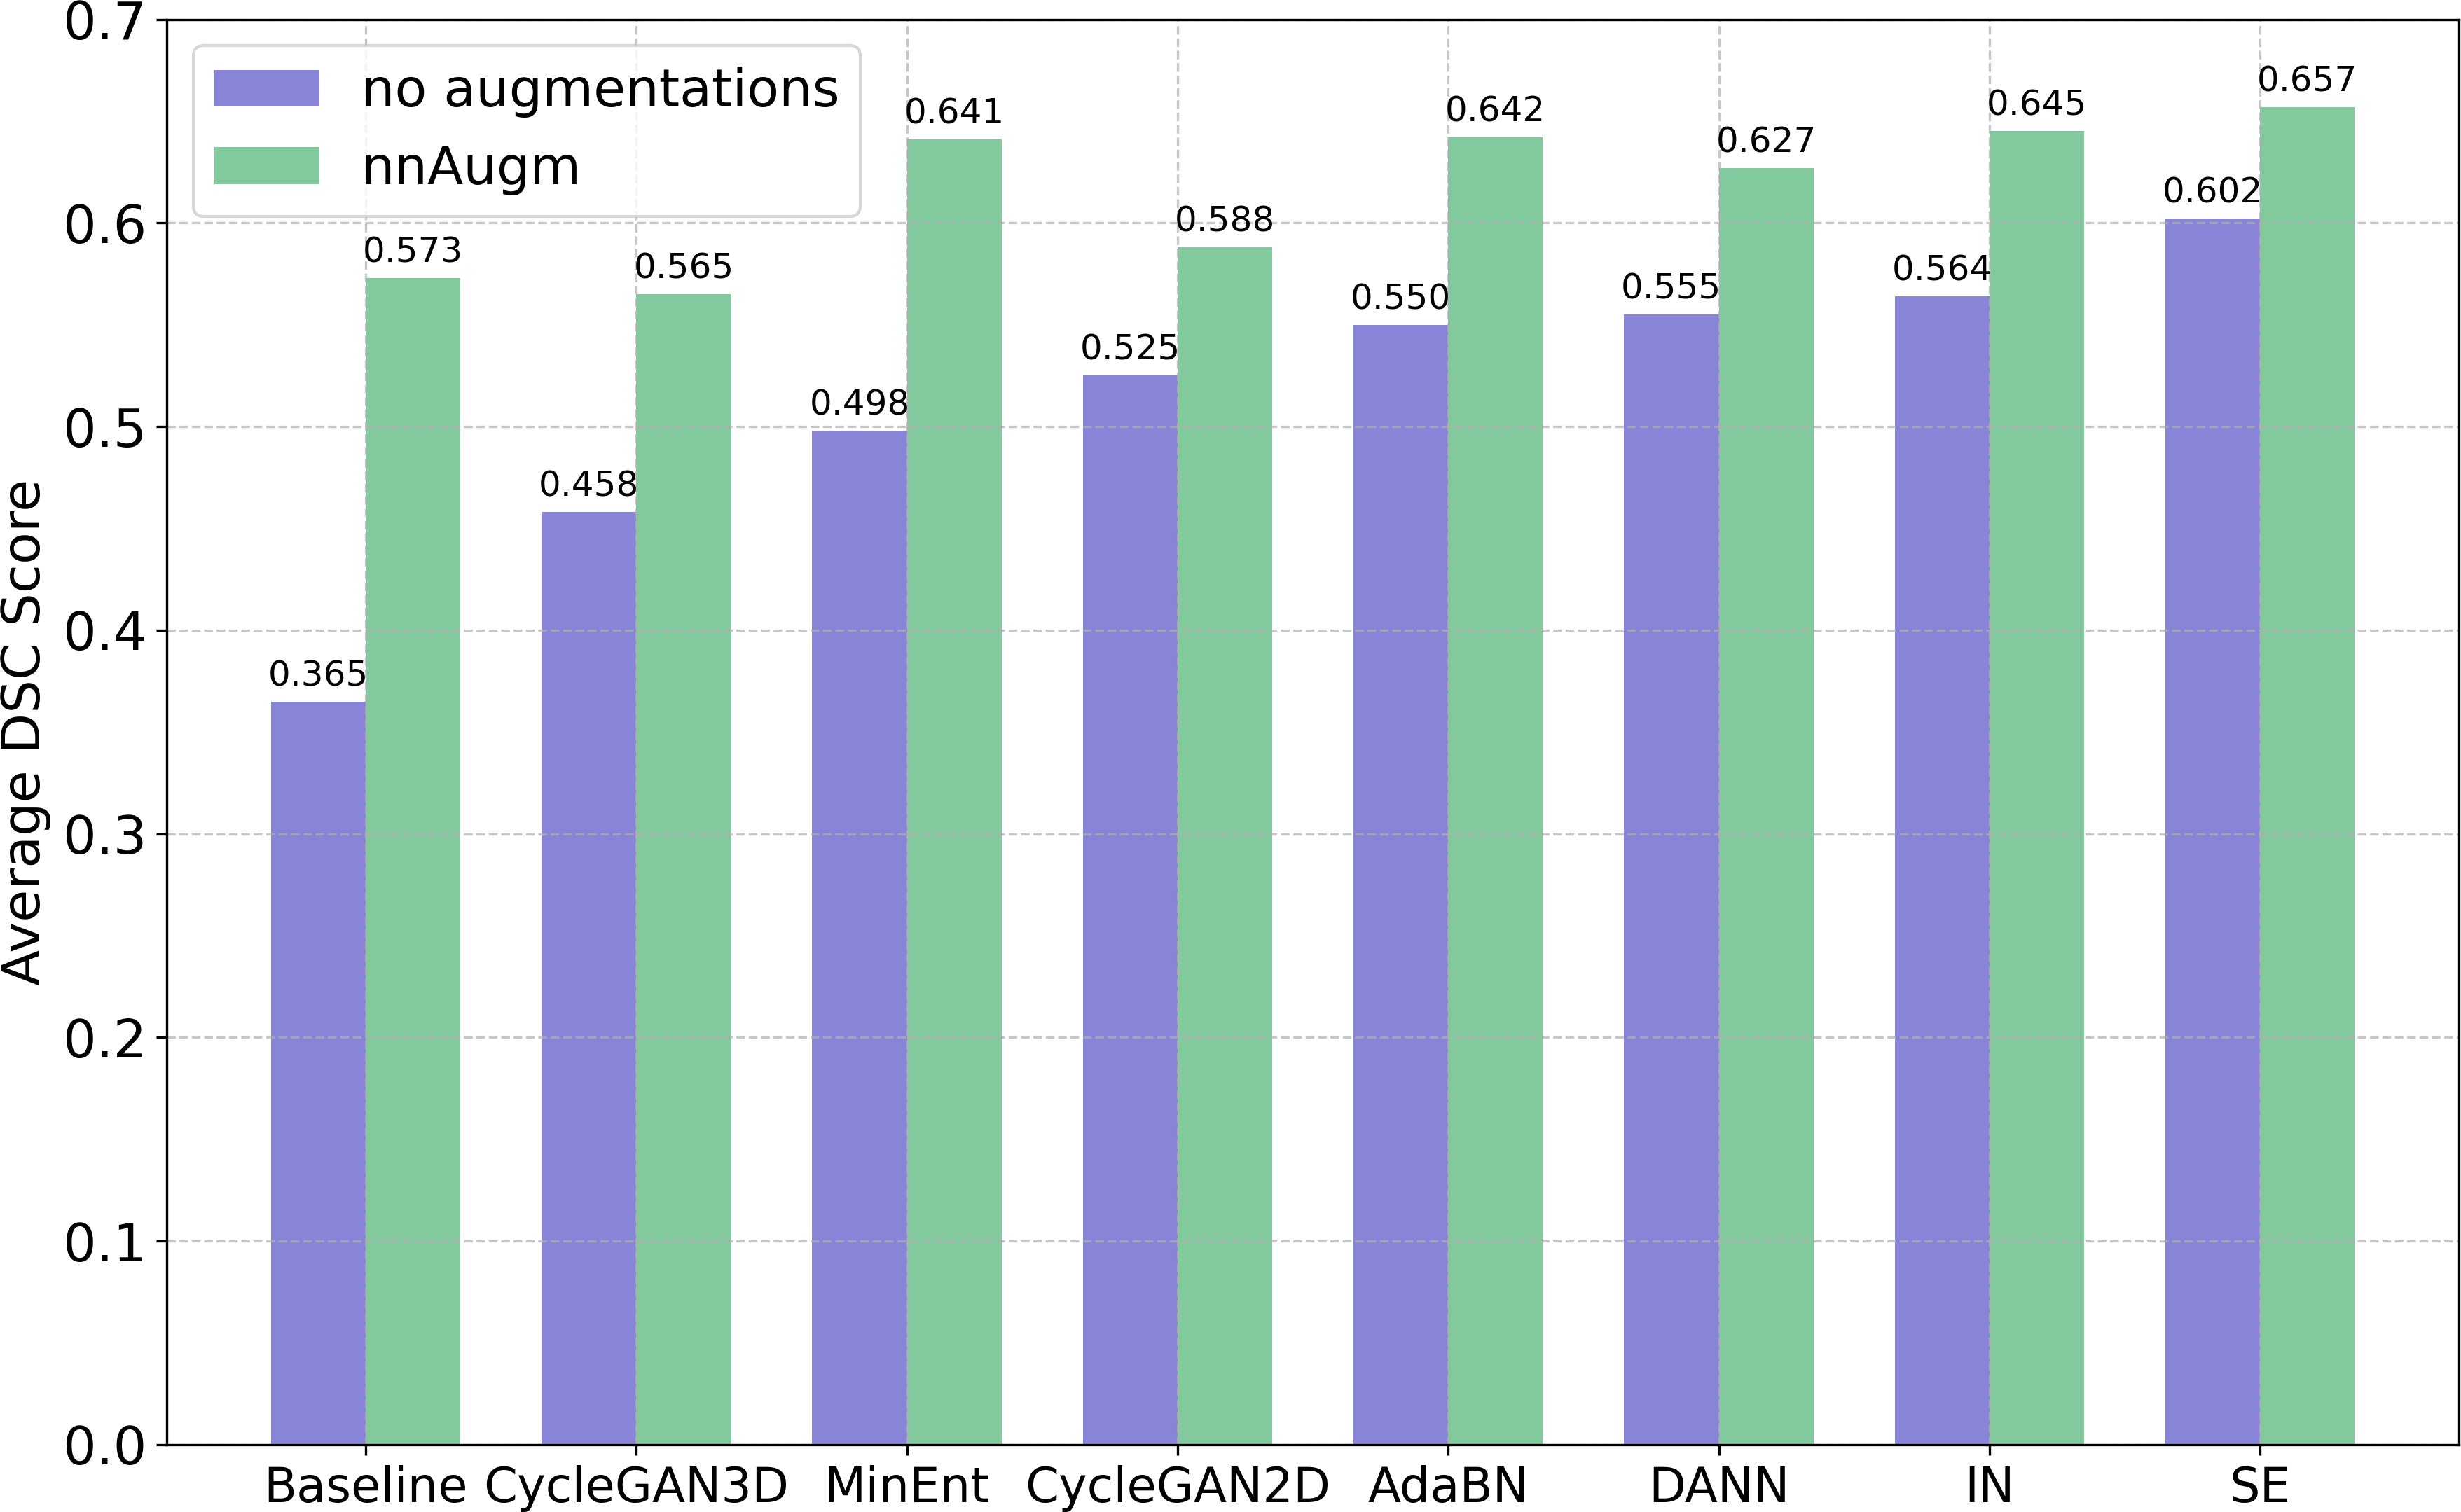
\includegraphics[width=1\linewidth]{Dissertation/Figures/4_da_bench/augm.png}
	\caption{Comparison of DA methods with and without augmentations.}
	\label{fig:augm}
\end{figure}

Finally, we systematically evaluated the effect of incorporating nnU-Net augmentations, nnAugm, into each domain adaptation method. Our results demonstrate consistent improvements across most methods (Figure~\ref{fig:augm}) and datasets (Table~\ref{tab:ablation_aug}), with an average increase of 10.3 percentage points in Dice score. These benefits varied significantly across different domain shifts: CT-related tasks showed the most substantial improvements, while MRI-based tasks exhibited more modest gains.

Different methods also showed varying degrees of improvement when supplemented with augmentations. MinEnt demonstrated the most dramatic enhancement, +33.5 percentage points in average gap, making it the best-performing method overall (Figure~\ref{fig:teaser1}). CycleGAN-based approaches also benefited significantly, especially in CT-related tasks. Self-Ensembling, while being the strongest initial method, showed the least improvement from the additional augmentations, suggesting that it might already benefited from the incorporated augmentations by design \cite{se_medim}. Notably, some methods exhibited slight performance degradation on specific tasks, indicating that aggressive augmentation strategies may occasionally interfere with method-specific adaptation mechanisms.

Viewing these results from the alternative perspective, we can consider each method as an additional adaptation strategy applied on top of the strong nnAugm baseline. From this point of view, the marginal benefit of adding sophisticated DA methods to an already well-augmented model is more modest but still significant. The best-performing methods (SE and MinEnt) provide an additional $10$--$15\%$ improvement over nnAugm, demonstrating that DA techniques can capture domain-specific variations that generic augmentations alone cannot address. This suggests that while extensive augmentations should form the foundation of any domain adaptation pipeline, method-specific adaptation mechanisms provide complementary benefits that warrant their inclusion in the final solution.

To conclude, despite significant advances in deep learning over the past decade, our benchmark reveals a concerning trend (Figure~\ref{fig:teaser3}): DA methods for medical image segmentation have shown minimal improvement since 2017, with recent approaches performing comparably or even worse than earlier ones, suggesting that closing the domain gap remains a fundamental challenge that requires radically new approaches.

\begin{figure}
	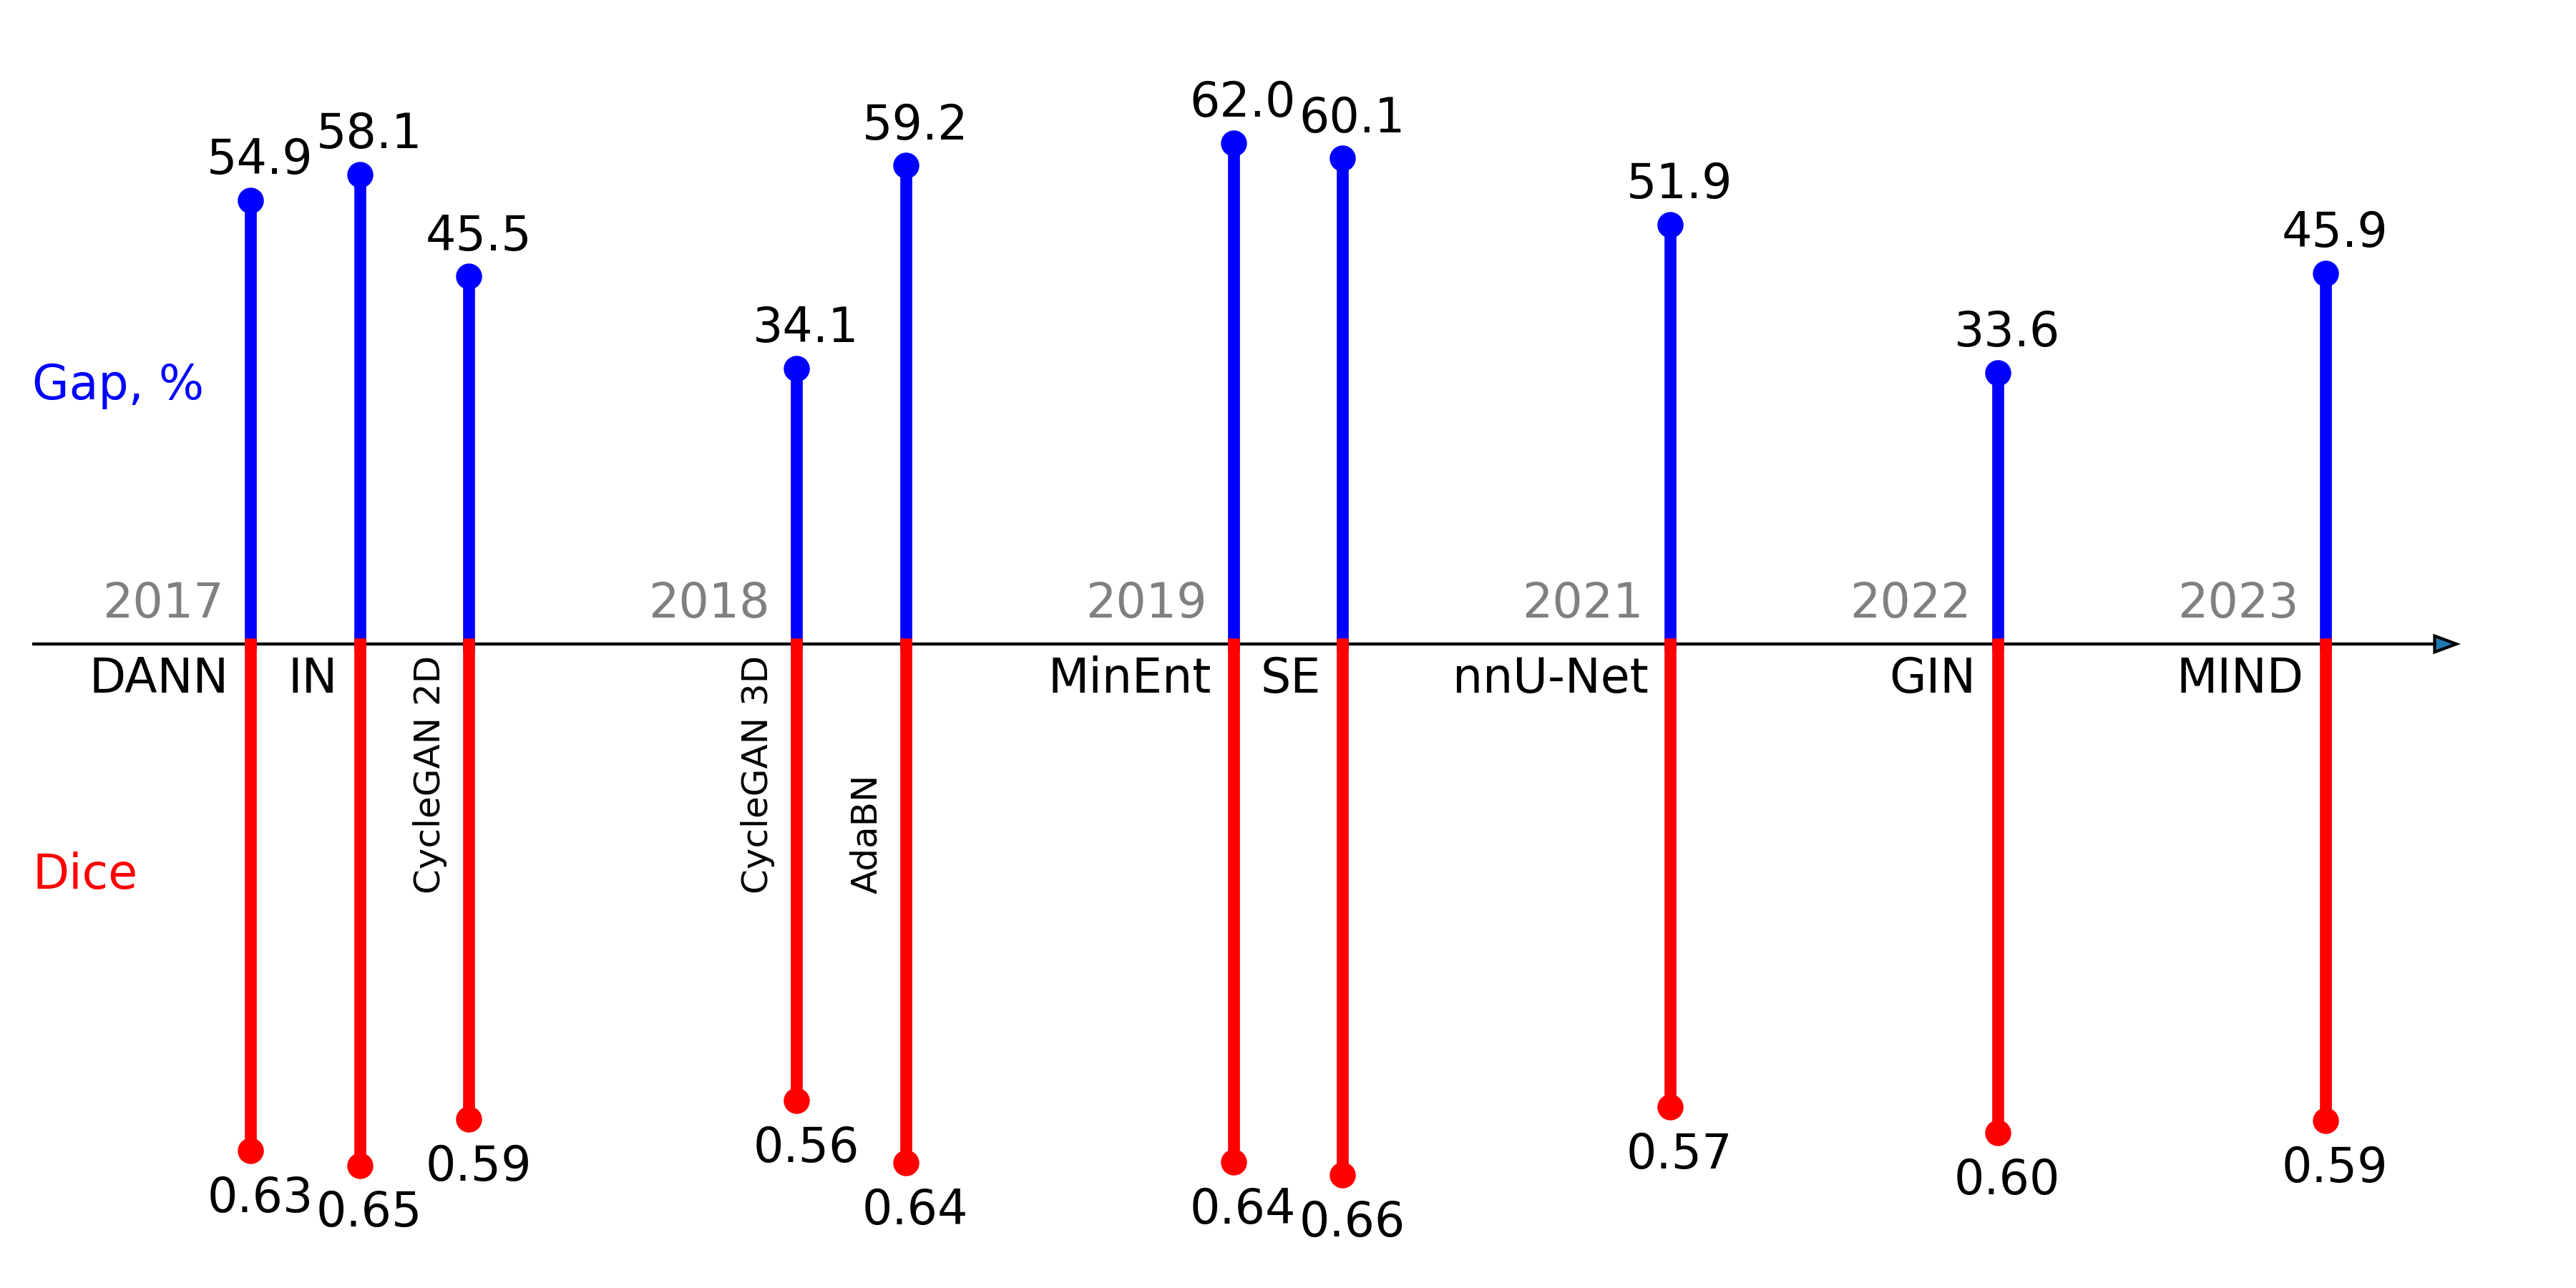
\includegraphics[width=\linewidth]{Dissertation/Figures/4_da_bench/cvpr_m3da_methods_timeline.png}
	\caption{Average performance of domain adaptation approaches on M3DA benchmark; see Table \ref{tab:ablation_aug} for detailed results.}  % objective progress being very little over time
	\label{fig:teaser3}
\end{figure}


\subsection{Supplementary experimental results}

Firstly, Table~\ref{tab:t1t2_soft_hard} provides the results in four domain shift setups which we excluded from the benchmark. Differences in CT reconstruction kernels were excluded due to relative simplicity (Baseline is only marginally worse than the Oracle, and extensive augmentations almost closes this gap). We also excluded the domain shift between T1 and T2 MRI sequences, because, we were not able to find enough clinical justification for the inclusion.



\begin{table}
	\centering
	\caption{Four setups not included in the M3DA benchmark.}
	
	\resizebox{1\textwidth}{!}{%
		\begin{tabular}{lcccc}
			\toprule
			& CT (soft) $\ra$ CT (sharp) & CT (sharp) $\ra$ CT (soft) & T1$\ra$T2 & T2$\ra$T1 \\
			
			\midrule
			
			\textit{Baseline} &  0.796	 &  0.819 &0.329 & 0.180  \\
			
			\midrule
			
			HM & --- & --- & 0.246 & 0.031 \\
			
			% CycleGAN 3D & --- & --- & --- & ---  \\
			
			MinEnt & --- & ---  & 0.322 & 0.094 \\
			
			CycleGAN 2D & --- & --- & 0.425 & 0.080  \\
			
			% GIN & --- & --- & --- & ---  \\
			
			AdaBN & --- & --- & 0.262 & 0.067 \\
			
			DANN &  --- & ---  & 0.228 & 0.028 \\
			
			IN &---	 & --- & 0.243 & 0.038 \\
			
			% MIND & --- & --- & --- & ---  \\
			
			Gamma & ---	 & ---	 & 0.288 & 0.132 \\
			
			SE & --- & --- & 0.000 & 0.000 \\
			
			nnAugm & 0.844 &	0.822 & 0.327 & 0.197 \\
			
			\midrule
			
			\textit{Oracle} &0.847 &0.845 & 0.728 & 0.686\\
			
			\bottomrule
			
	\end{tabular}}
	\label{tab:t1t2_soft_hard}
\end{table}




\section{Discussion}

While we focused our computational experiments on unsupervised DA, M3DA also supports other DA frameworks.

\paragraph{Supervised DA} involves having annotated data from source and target domains. It can potentially close the performance gap more effectively, leveraging the explicit knowledge of target domain characteristics. All datasets and samples in M3DA come with segmentation annotations, allowing supervised DA setup.

\paragraph{Source-free DA} In this setting, the model is trained on the source domain and later adapted to the target domain without accessing source data. This approach is particularly relevant in scenarios with privacy concerns. M3DA allows source-free DA by removing the source data during finetuning.

\paragraph{Test-time DA} focuses on adapting the model during inference. This method adjusts to the target domain using only the data available at the inference time. Similar to source-free DA, one can limit access to the source domain and use online sampling of the target data.

\paragraph{Domain Generalization (DG)} aims to learn domain-invariant features from multiple source domains without accessing any target domain data during training. This approach is particularly valuable in medical imaging where encountering completely new domains is common, such as images from different hospitals or scanner manufacturers. M3DA's diverse collection of datasets from various medical centers and imaging protocols\footnote{LIDC is sourced from seven academic centers and eight medical imaging companies, BraTS is sourced from at least nine different clinical centers, AMOS was collected in two medical centers, from eight different scanners} makes it well-suited for developing and evaluating DG methods.

These alternative DA frameworks showcase the versatility of our benchmark and its potential to support a wide range of research questions and methodologies in the field of domain adaptation for medical image segmentation.


\subsection{Limitations and Future Directions}
\label{sec:da_bench:exp:limitations}

While we incorporate a diverse set of domain shifts, our benchmark is not exhaustive. We exclude several candidate domain shifts due to their simplicity, low relevance, or lack of available public data. First, the CT reconstruction kernel (from sinogram space to voxel space) is an important parameter. As shown in \cite{fbpaug}, this problem can be largely mitigated via simple augmentations or an auxiliary loss function \cite{shimovolos2022adaptation}. We include our results on this shift in Supplementary materials, but as it is almost fully addressed by simple augmentations, we exclude it from the main benchmark. Also, public datasets containing both reconstruction kernel information and segmentation annotations are scarce.

Second, the CC359 dataset consists of data from six distinct domains, allowing for 30 different domain shift scenarios. We selected the three least ``solved'' shifts based on our preliminary analysis. A complete table with results on all 30 domain pairs is provided in Appendix~\ref{app:m3da_datasets}, Table~\ref{tab:wmgmcsf}.

Third, a common critique of the BraTS dataset is that it is heavily preprocessed. Incorporating raw datasets could provide an evaluation of DA methods in a more realistic setting. However, this comes with an inevitable trade-off of added complexity in data preparation. Addressing this issue specifically, we collected and published the BGP dataset~\cite{Zolotova2023Burdenko}, see Section~\ref{sec:da_bench:bgpd} below.

% We also exclude the MRI T1 to T2 domain shift from the main paper. Although we provide the results for this setup in Supplementary materials, we did not find sufficient evidence to support its clinical relevance, leading to its exclusion from our benchmark.

Finally, while the LIDC dataset allows for the CE CT to CT shift, it is primarily designed for object detection tasks, with multiple nodules per image. Despite this limitation, LIDC remains the only publicly available dataset of sufficient size that enables this clinically relevant domain shift.

Future work should focus on expanding M3DA to include more clinically relevant domain shifts, incorporating datasets with unprocessed scans, and exploring novel approaches to domain adaptation.


\section{Burdenko's Glioblastoma Progression Dataset}
\label{sec:da_bench:bgpd}

As we have shown, many researchers develop DA methods tailored to specific types of domain shifts, which limits their ability to generalize across other clinically relevant variations. Even when a method demonstrates uniformly strong performance within the proposed M3DA benchmark, its effectiveness should be validated on a diverse and clinically representative dataset. As an example, one might take the glioblastoma segmentation task, where data is inherently heterogeneous, originating from scanners with different imaging protocols, manufacturers, and varying clinical objectives.

There is an increased interest in automating brain glioma segmentation, facilitated by a BraTS competition~\cite{brats}, whose organizers published pre-operative images of about 2000 subjects with manual (and semi-automatic) segmentation maps of tumor core, enhancing tumor and peritumoral edema, since 2014. Concurrently, there are almost no annotated data collections for contouring gross tumor volume (GTV) on MRI for radiotherapy planning~\cite{menze2021analyzing}. All publicly available datasets are of a small scale of the order of a few dozen patients. Our study is going to partially close this gap.

Furthermore, to highlight difficulties in applying existing algorithms to a related (but a different) task, we demonstrate the performance of competition-winning solutions on a new domain. We assess the complexity of the GTV contouring task by benchmarking five award-winning solutions (in different years) of the BraTS competition on our dataset~\cite{kofler2020brats,isensee2018nnu,kickingereder2019automated,bakas2017advancing}. All algorithms show a significant deterioration in the performance compared to the original task, ranging between 0.40 up to 0.70 Dice score on the GTV annotation task (compared to 0.79 up to 0.90 on the original pre-operative images). This result indicates that although the problems are related (same pathology, same image modalities, same algorithm), solving one does not solve the other.


So we publish the Burdenko's Glioblastoma Progression (BGP) dataset, a systematic data collection of pre-radiotherapy MRI images of 180 patients with primary glioblastoma who undergo treatment at the Burdenko National Medical Research Center of Neurosurgery from 2014 to 2019. For each patient, the dataset includes imaging studies conducted for radiotherapy planning and follow-up studies. The radiotherapy studies consist of 4 MRI sequences (T1, T1C, T2, FLAIR), a topometric CT scan, and associated radiotherapy planning files (RTSTRUCT, RTPLAN, and RTDOSE). Follow-up studies (from 1 to 8-time per patient) include 2-4 MRI sequences (with a minimal set of T1C and FLAIR) per patient. See data examples in Figure~\ref{fig:gbpd}. %Additional genetic information and a treatment response status (tumour progression, tumour pseudoprogression, treatment response) are available for a subset of patients.

\begin{figure}
	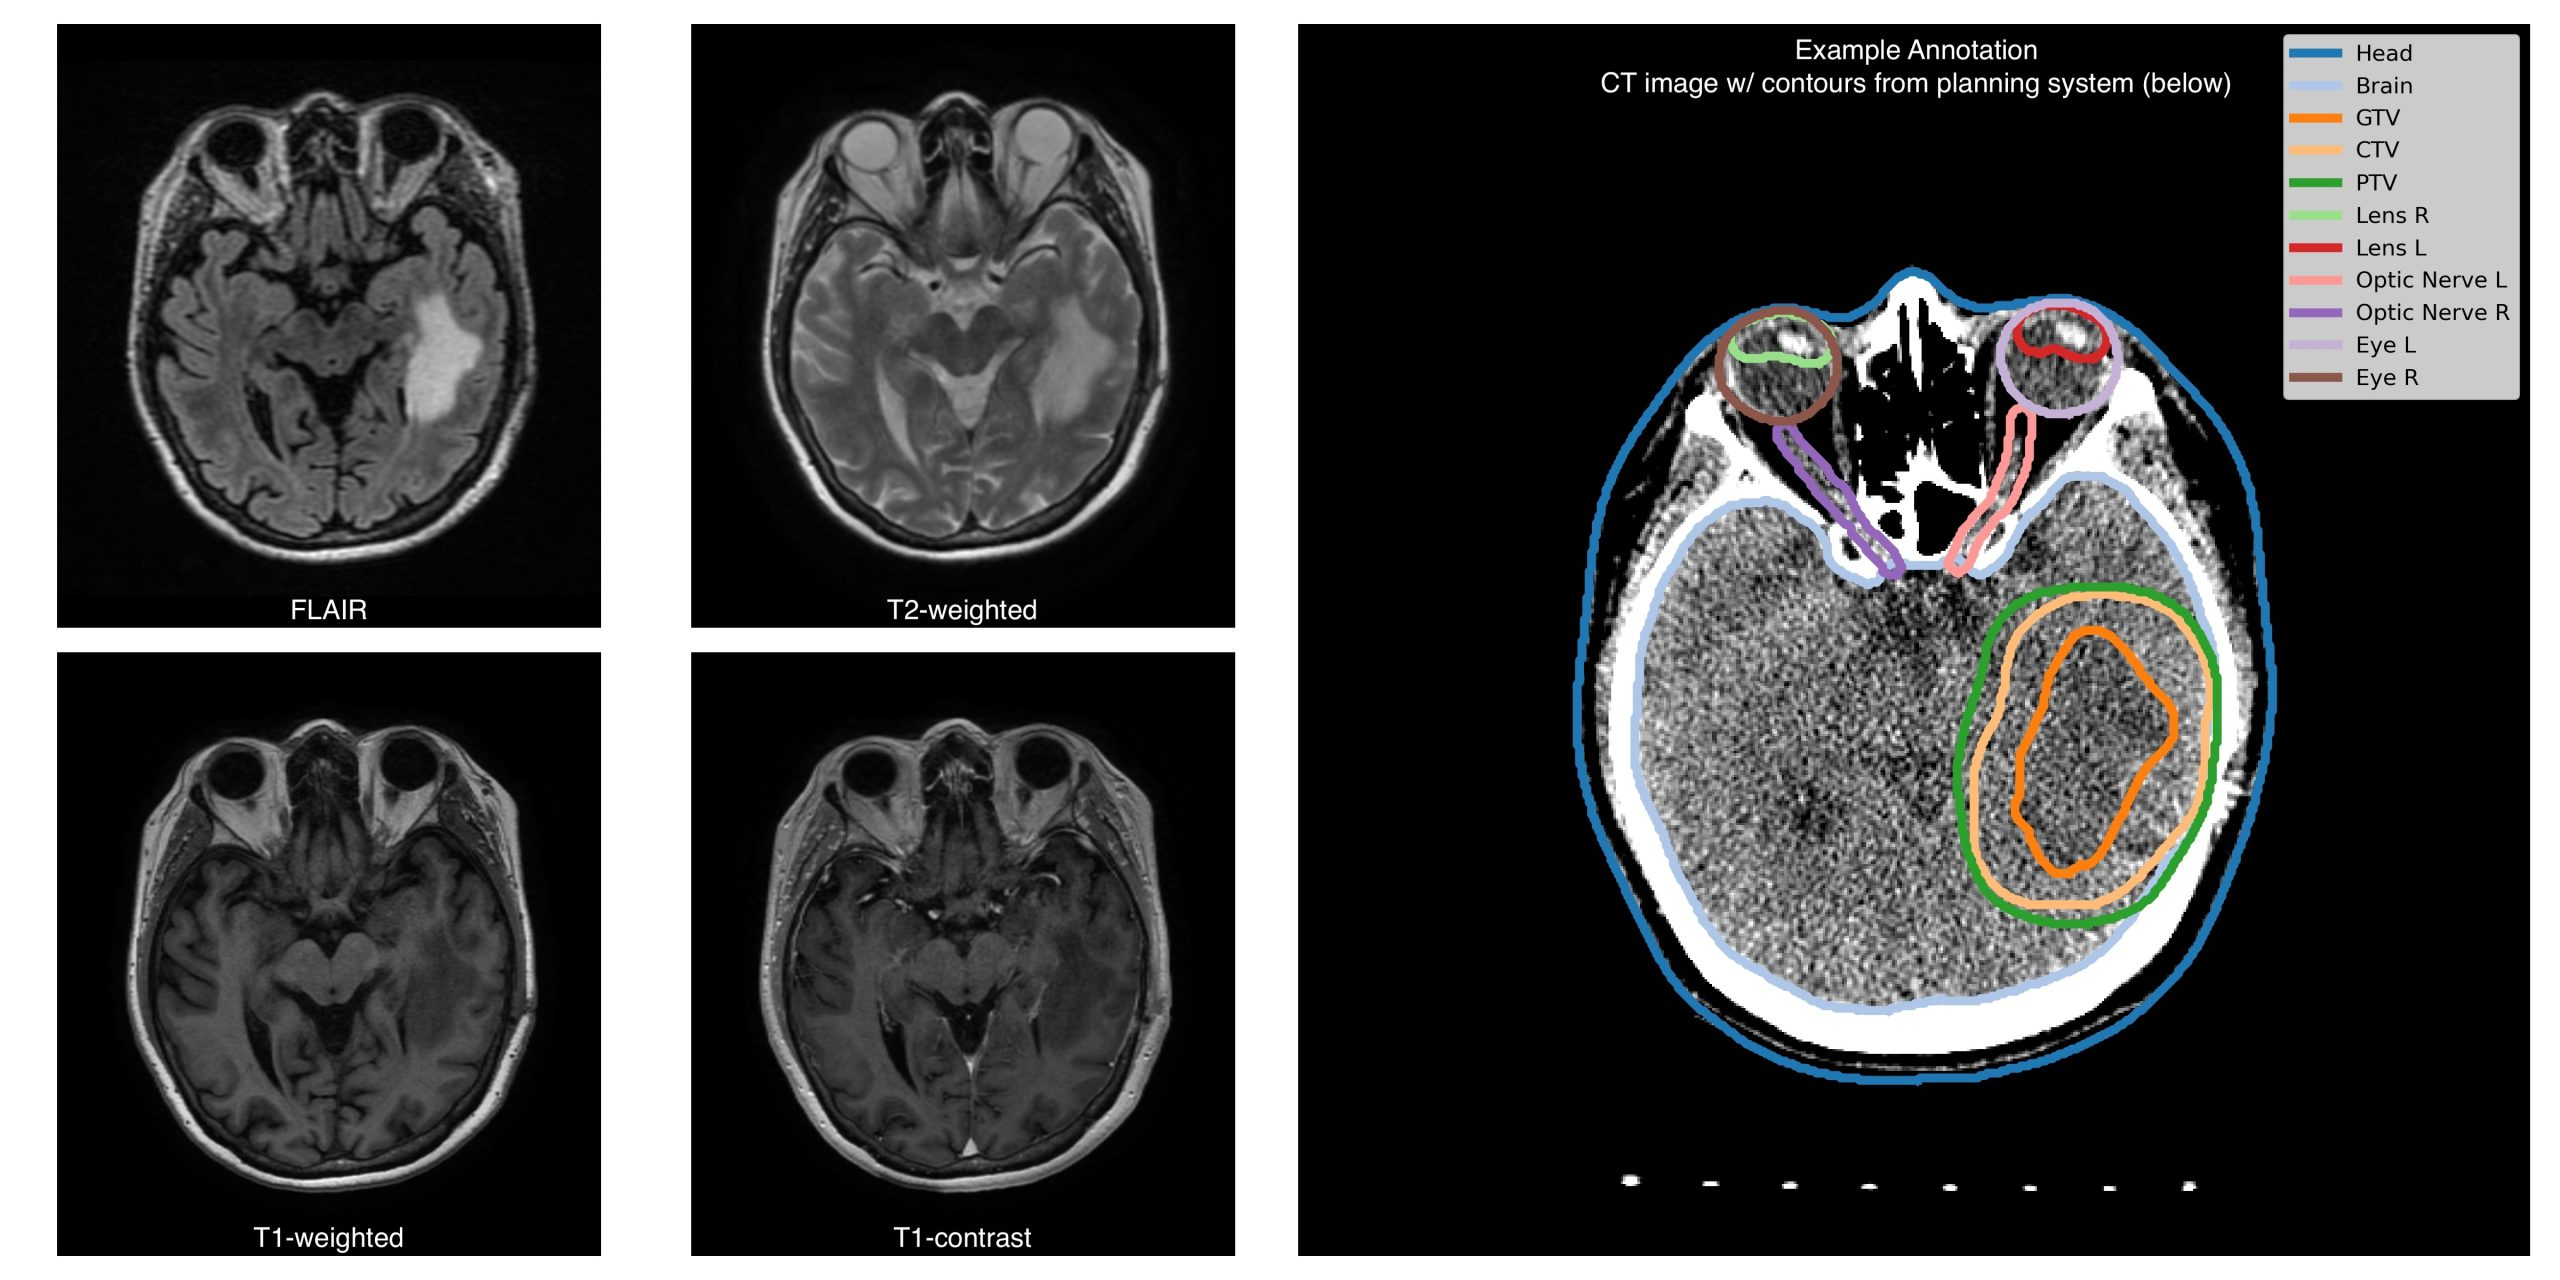
\includegraphics[width=\linewidth]{Dissertation/Figures/4_da_bench/Burdenko-GBM-Progression-scaled.jpg}
	\caption{A data sample from the Burdenko's Glioblastoma Progression dataset.}
	\label{fig:gbpd}
\end{figure}


The MRI studies were obtained from different sites, with scanners from four vendors and varying scanning protocols. %CT studies were obtained using a unified scanning protocol.
By introducing the BGP dataset, we provide, among other contributions, a realistic ``in-the-wild'' domain adaptation setup, where segmentation models must generalize across diverse acquisition conditions and clinical scenarios.


\section{Summary}

In this chapter, we introduced the M3DA benchmark for unsupervised domain adaptation in 3D medical image segmentation. Addressing the widely indicated need for developing DA methods in the medical imaging domain, as emphasized in recent literature~\cite{gulrajani2020search,uda_survey_2020,zhuang2020comprehensive,peng2018visda,zhang2021empirical}, we created a large-scale benchmark to facilitate the development of robust segmentation methods in such a crucial application area. Contrary to previously used setups, we covered a diverse set of domain shift sources while using large, publicly available datasets.

We benchmarked the core adaptation methods, covering all key categories of unsupervised DA approaches \cite{medim_da_survey_2021,medim_da_survey_2023}, and medical foundational models. Our results revealed that adapted segmentation models struggle to generalize beyond their training distribution when tested at scale. Although some DA methods showed promise in particular settings, we revealed they might completely fail in a number of other setups. This highlights a pressing need for creating robust methods for medical image segmentation, and we hope to foster research efforts in improving adaptation methods’ performance in diverse situations.

To further support research in clinically relevant and scalable DA, we introduced and published the Burdenko's Glioblastoma Progression (BGP) dataset, a data collection of pre-radiotherapy MRI studies from multiple clinical sites. The dataset reflects real-world imaging heterogeneity, including scans from four different MRI vendors with varying protocols. Our evaluation of state-of-the-art glioblastoma segmentation models demonstrated a substantial performance drop when applied to this heterogeneous data. Thus, the BGP dataset provides an essential realistic ``in-the-wild'' DA setup, bridging the gap between methodological research and practical deployment.


Finally, we suggested various alternative problem settings within the M3DA benchmark, such as supervised and test-time DA. These settings allow for the evaluation of more complex hypotheses across a broader spectrum of DA methods, encouraging further research into improving adaptation performance in diverse medical imaging contexts.



\begin{figure}[h]
	\centering
	\includegraphics[width=1\linewidth]{Dissertation/Figures/4_da_bench/preds.png}
	\caption{Example predictions for different DA methods. Methods are in rows, starting with ground truth in a first row. All eight benchmark tasks are in columns.}
	\label{fig:predicts}
\end{figure}



	

\chapter{Benchmark for OOD in 3D Medical Image Segmentation}
\label{chap:ood_bench}


Deep Learning (DL) models perform unreliably when the data come from a distribution different from the training one. Above, we have investigated adaptation to the different data distribution, assuming the latter is predefined. In this chapter, we complement our investigation with the detection of novel data distributions. Out-of-distribution (OOD) detection methods help to identify novel data samples with a possibility to prevent erroneous predictions instead of marginally improving performance in the case of adaptation. So we investigate OOD detection effectiveness when applied to 3D medical image segmentation. We designed several OOD challenges representing clinically occurring cases and found that none of the methods achieved acceptable performance. We released the designed challenges as a publicly available benchmark and formulated several criteria to test the generalization of OOD detection beyond the suggested benchmark.

The results presented in this chapter are based on the author’s publication~\cite{vasiliuk2023limitations}.

%In critical applications such as medical imaging, out-of-distribution (OOD) detection methods help to identify such data samples, preventing erroneous predictions. So we investigate OOD detection effectiveness when applied to 3D medical image segmentation. We designed several OOD challenges representing clinically occurring cases and found that none of the methods achieved acceptable performance. Our findings highlight the limitations of the existing OOD detection methods with 3D medical images and present a promising avenue for improving them. To facilitate research in this area, we release the designed challenges as a publicly available benchmark and formulate practical criteria to test the generalization of OOD detection beyond the suggested benchmark.

% Methods not dedicated to segmentation severely failed to perform in the designed setups; the best mean false-positive rate at a 95\% true-positive rate (FPR) was 0.59. Segmentation-dedicated methods still achieved suboptimal performance, with the best mean FPR being 0.31 (lower is better). To indicate this suboptimality, we developed a simple method called Intensity Histogram Features (IHF), which performed comparably or better in the same challenges, with a mean FPR of 0.25.
%  We also propose IHF as a solid baseline to contest emerging methods.


\section{Background}

%In recent years, deep learning (DL) methods have achieved human-level performance in automated medical image processing. However, the development of these methods on a large scale is slowed by several factors. One such factor is the unreliable performance of DL models when the data come from a distribution different from the training one \cite{wang2018deep}. These differences are common in medical imaging: population, demographic, or acquisition parameter changes or new imaging modalities.

One of the factors limiting development of DL methods in medical image processing is when the data come from a distribution different from the training one. These differences are common in medical imaging: population, demographic, or acquisition parameter changes or new imaging modalities. OOD detection helps to identify the data samples with such differences, hence increasing the reliability and safety of a DL model. For instance, detected cases could be marked as rejected, preserving the model performance, or reported to the experts, preventing the model from failing silently. The ability to report or reject unreliable cases is now considered a necessary capability to enable safe clinical deployment \cite{kompa2021second}.

% for X-Rays \cite{berger2021confidence}, skin cancer photos \cite{pacheco2020out}, axial slices of brain MRI \cite{mahmood2020multiscale}
OOD detection with natural images is a well researched area \cite{yang2024generalized} where several established benchmarks \cite{hendrycks2016baseline,basart2022scaling} facilitate its development. Moreover, these methods directly scale to 2D medical images, resulting in multiple algorithms \cite{mahmood2020multiscale,pacheco2020out,berger2021confidence} and also a benchmark \cite{cao2020benchmark}. At the same time, OOD detection with 3D medical images remains poorly explored, although 3D medical image segmentation is one of the most addressed tasks in medical imaging \cite{medim_dl_survey_2017} with outstanding practical usefulness; e.g., diagnostics, quantifying anatomical structures, pathologies, or important biomarkers.

The primary cause of this poor exploration is the lack of datasets and benchmarks with a correct problem design. For example, one party may use private data \cite{karimi2022improving}, while another simulates synthetic anomalies that are unlikely to occur in clinical settings \cite{david_zimmerer_2022_6362313}. A study can be limited to a single distribution shift (e.g., changes in the scanning location \cite{karimi2022improving}), thus lacking the diversity of setups. Also, studies may be restricted to uncertainty estimation~\cite{lambert2022improving} or anomaly detection \cite{david_zimmerer_2022_6362313} methods, leaving the full spectrum of approaches uncovered. Such issues limit the fair comparison of the proposed approaches.

% correct methodology / problem setting
In this chapter, we investigate the effectiveness of OOD detection when applied to 3D medical image segmentation, closing the outlined gaps in prior work. To enable a correct comparison, we thus designed a diverse set of challenges using publicly available data with a downstream segmentation task and simulation of clinically occurring anomaly sources. Besides the problem design, such a study requires appropriately selected state-of-the-art methods. We note that several areas (e.g., anomaly detection and uncertainty estimation) share motivation and methodology with OOD detection. Therefore, we review all related areas and, in contrast to the previous works, present complete methodological coverage.

Extensive evaluation of six selected methods resulted in our main conclusion: state-of-the-art OOD detection falls short of achieving optimal performance with 3D medical images. We show that the methods not designed for segmentation completely failed in most setups, scoring from $0.84$ to $0.59$ for the false-positive rate (FPR) on average, which was not far below the $0.95$~FPR of the random guessing (a lower FPR is better.) Two methods specifically designed for 3D segmentation achieved $0.38$ and $0.31$ mean FPRs, further reducing the error by about two times. At the same time, we show that these errors can be reduced even further with a simple approach.

We show this space for improvement by developing a histogram-based method called Intensity Histogram Features (IHF). IHF achieved comparable and often superior results to its competitors, with a $0.25$ mean FPR. It also scored $0$ for the FPR in multiple challenges, indicating that the distribution shifts in 3D medical imaging can often be detected using image intensity histograms, while the DL-based methods overlook this domain feature. Therefore, we consider current DL-based OOD detection to be far from unveiling its full potential and assume it can be further improved.
% method as a part of methodology
% For example, we can incorporate the histogram information into the network.

Given IHF's negligible computational costs compared to DL, we suggest it as a baseline to contest the emerging OOD detection methods. Furthermore, we propose using the designed challenges as a benchmark for developing new methods. Correct problem setting; in-depth analysis with simple methods, such as IHF; and ablation studies with synthetic data confirm that our benchmark makes it possible to estimate the quality of implementing general OOD detection instead of classifying a priori known anomaly types.% Thus, summarizing our contributions, we outline the following:
% or a starting point to create a more refined one

%\begin{enumerate}	
%	\item We demonstrate the severe limitations of the existing OOD detection methods with 3D medical images.% and indicate a space for improving them.	
%	\item We designed and now release the corresponding benchmark that can be used as a starting point for related research. % formulate practical criteria
%	\item We propose a method, IHF, and suggest it as a solid baseline for OOD detection with 3D medical images.% and a resource-efficient tool for analyzing related datasets. 	
%\end{enumerate}

%Below, we describe the data used in our study and the problem setup (Section~\ref{sec:data}). Then, we review and select state-of-the-art and core methods from the related fields and also detail IHF (Section~\ref{sec:methods}). Finally, we present the results (Section~\ref{sec:results}) and discuss the limitations and implications of our study (Section~\ref{sec:discussion}).


\section{Data}

In contrast to the fields of 2D natural and medical images, no established OOD detection benchmark with a correct problem setting exists for 3D medical images. For example, Karimi et al. \cite{karimi2022improving} used a variety of brain and abdominal CT and MRI datasets but included private ones. The authors also studied only a single distribution shift, changes in the scanning location, which did not allow the estimation of the general performance. Zimmerer et al. \cite{david_zimmerer_2022_6362313} created an OOD detection challenge by simulating synthetic anomalies in brain MR and abdominal CT images. However, their setup lacks a downstream task (e.g., segmentation), so the study is limited to unsupervised anomaly detection methods. Synthesis of local corruptions, as in \cite{david_zimmerer_2022_6362313}, can also lead to evaluation biases, which we show with our analysis. On the other hand, Lambert et al. \cite{lambert2022improving} included datasets with a segmentation task but limited the considered methods to supervised uncertainty estimation.

Given the disagreement of setups, partial problem coverage, or privacy, we designed the OOD detection challenges from scratch following three core principles:

\begin{itemize}
	
	\item We included two large \textit{publicly available} CT and MRI in-distribution (ID) datasets to cover the most frequent volumetric modalities.
	
	\item We ensured both datasets had \textit{a downstream segmentation task}, allowing us to use the full spectrum of methods.
	
	\item We selected \textit{diverse} OOD datasets that simulated the \textit{clinically occurring sources of anomalies}: changes in acquisition protocol, patient population, or anatomical region. All these datasets are publicly available.
	
\end{itemize}

We also synthesized several medical imaging artifacts as anomaly sources. Generating synthetic anomalies is a popular approach, applied for 3D images \cite{david_zimmerer_2022_6362313,lambert2022improving} as well as 2D images \cite{hendrycks2016baseline,basart2022scaling}; this approach also allowed us to conduct controlled ablation studies at different distortion levels.

%We made the resulting benchmark publicly available ({\url{https://github.com/francisso/OOD-benchmark}}, last accessed 13.09.23).
All related CT and MRI datasets and the problem setting are detailed below.


\subsection{Lung Nodules Segmentation}

We constructed a total of 6 challenges on CT data, including two synthetic ones.

\textbf{ID dataset.} As an ID dataset, we used LIDC-IDRI \cite{lidc}. It contains 1018 chest CT images with the lung nodules segmentation task. We removed cases without nodules since they do not contribute to training a segmentation model. Then, we randomly split the remaining 883 images 4:1 into the train and test, stratified by the number of nodules.

\textbf{OOD source: \textit{scanner}.} To simulate a covariate shift, we selected Cancer500 \cite{morozov2021simplified} which has the same downstream task as the ID dataset but is obtained with different scanners and acquisition protocols. It contains 841 chest CT images, excluding images with low resolution (less than 64 axial slices) and no annotated nodules.

\textbf{OOD source: \textit{population}.} To simulate a patient population shift, we used two datasets with similar semantic content but different downstream task: Medseg9 and MIDRC \cite{tsai2021rsna}. They contain 9 and 154 chest CT images, respectively, with COVID-19 cases. Excluding all non-COVID cases, the merged dataset has 120 images.

\textbf{OOD source: \textit{location (liver)}.} To simulate a semantic shift, we selected a dataset of the same modality but a different body region. Here, we used LiTS \cite{bilic2023liver}, a dataset with 201 abdominal CT images.

\textbf{OOD source: \textit{location (head)}.} Similarly, we included CT-ICH \cite{hssayeni2020computed}, a dataset with 75 head CT images.

\textbf{OOD source: \textit{synthetic (image noise)}.} We simulated local image corruptions by applying damaging transformations to the test cases of the ID dataset. The transformations include blurring, changing image contrast, or inserting Gaussian noise in a randomly selected image crop.

\textbf{OOD source: \textit{synthetic (elastic)}.} We simulated tissue anomalies by applying an elastic transform of random severity.



We give visual examples of data samples in Figure~\ref{fig:ood_examples}~(top row).%Segmentation quality of the downstream model is provided in Table~\ref{tab:segm_ct}.

\begin{landscape}
	\begin{figure}[p]
		\centering
		\begin{minipage}{\linewidth}
			\centering
			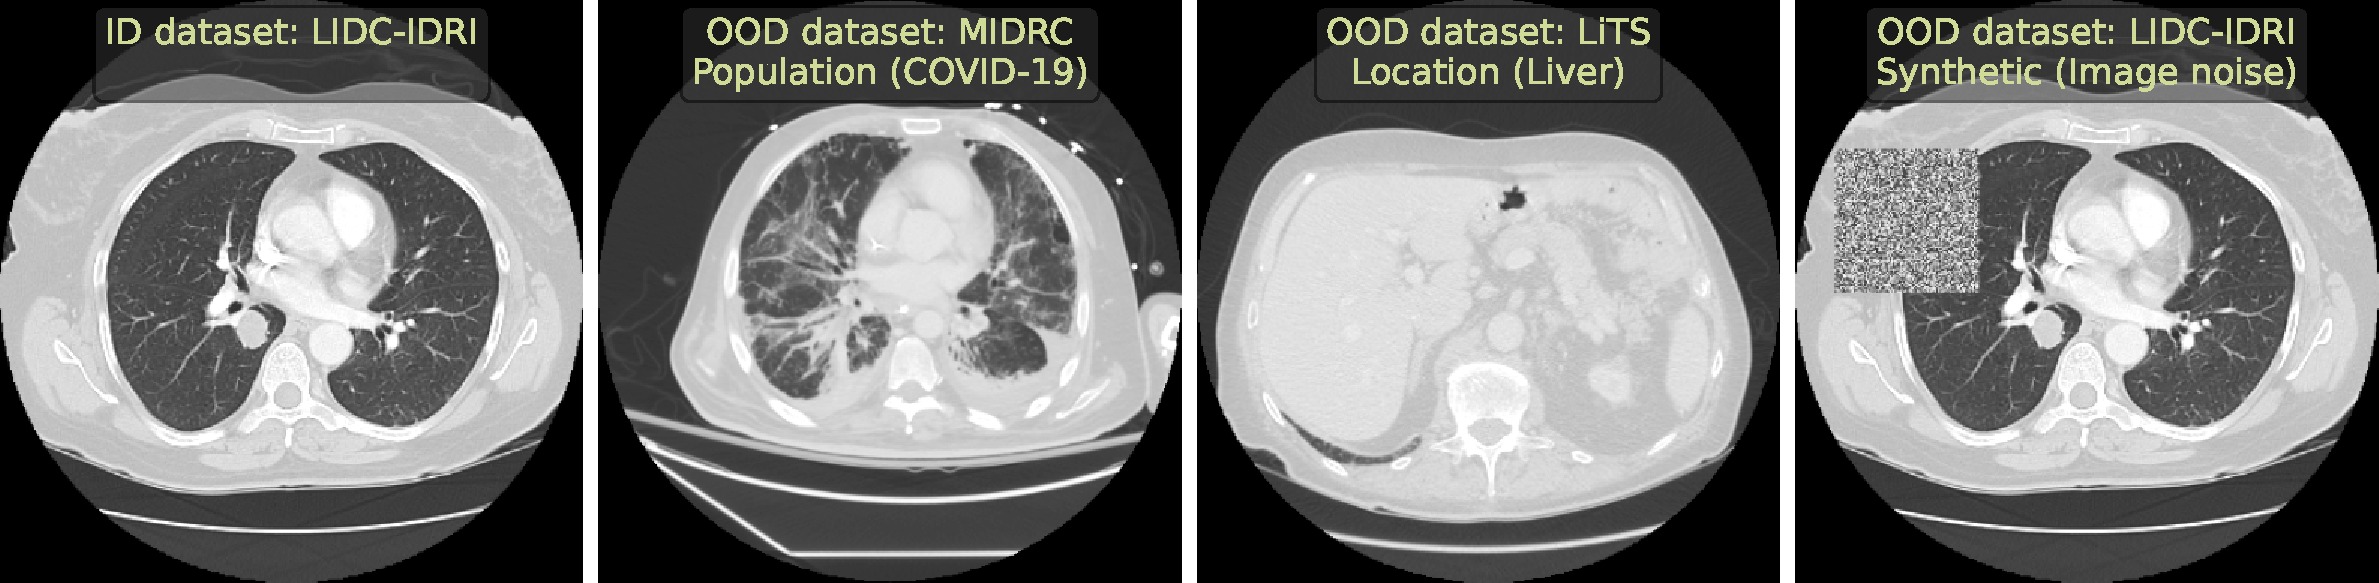
\includegraphics[width=\linewidth]{Dissertation/Figures/5_ood_bench/ct_examples_2.pdf}
			
			\vspace{0.5em} % small vertical gap between rows
			
			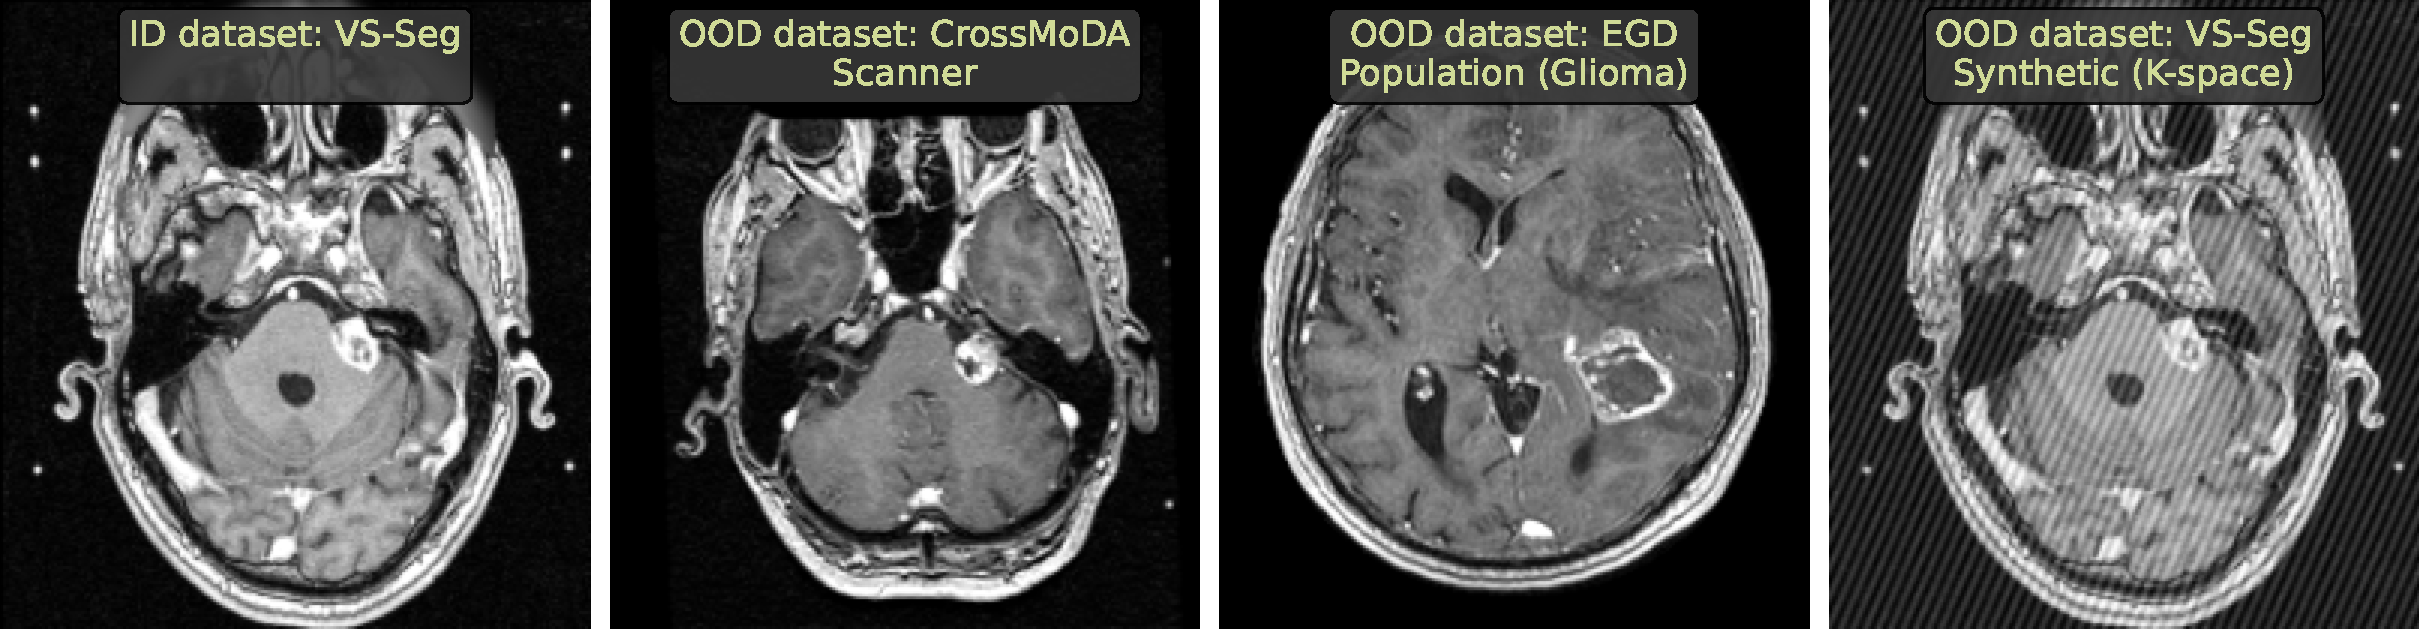
\includegraphics[width=\linewidth]{Dissertation/Figures/5_ood_bench/mri_examples_2.pdf}
		\end{minipage}
		\caption{Examples of (top row) CT and (bottom row) MRI images from different simulated OOD sources in our benchmark.}% (representative axial slices)
		\label{fig:ood_examples}
	\end{figure}
\end{landscape}


%

%\begin{table}[H]
%	\caption{Segmentation quality in the considered CT setups. We provide Dice score (DSC, higher is better $(\uparrow)$) and average number of false-positive detections per image (Avg. FP, lower is better $(\downarrow)$) as our metrics.}
%	\begin{adjustwidth}{-\extralength}{0cm}
%		\centering %% If there is a figure in wide page, please release command \centering
%		%\vspace{.2cm}
%		{%
%			\begin{tabularx}{\fulllength}{lCCCCcCC}
%				\toprule
%				\multirow{2}{*}[-0.2em]{\textbf{Metric}} & \textbf{ID Dataset} & \multicolumn{6}{c}{\textbf{OOD Challenges}} \\
%				\cmidrule{2-8}
%				
%				& \textbf{LIDC} & \textbf{Loc (Head)} & \textbf{Loc (Liver)} & \textbf{Scanner} & \textbf{Pop (COVID)} & \textbf{Syn (Noise)} & \textbf{Syn (Elastic)} \\
%				
%				
%				\midrule
%				DSC $(\uparrow)$ & $0.50 \pm 0.27$ & $0.21 \pm 0.41$ & $0.03 \pm 0.16$ & $0.18 \pm 0.24$ & $0.00 \pm 0.00$ & $0.32 \pm 0.30$ & $0.13 \pm 0.23$ \\
%				
%				
%				Avg. FP $(\downarrow)$ & $5.2 \pm 6.9$ & $2.6 \pm 4.6$ &  $10 \pm 16$ & $ 6 \pm 15$ & $13 \pm 10 $ & $12\pm 25$ & $5.4 \pm 4.5$ \\
%				
%				
%				% avg FP $(\downarrow)$ & $3.6 \pm 0.5$ & $2.9 \pm 0.9$ & $10.5 \pm 1.4$ & $6.1 \pm 0.7$ & $12.0 \pm 4.0$ & $12.3 \pm 1.2$ & $13.8 \pm 1.3$ & $4.6 \pm 0.8$\\
%				\bottomrule
%		\end{tabularx}}
%	\end{adjustwidth}
%	\label{tab:segm_ct}
%\end{table}


\begin{table}[h]
	\centering
	\caption{Segmentation quality in the considered CT setups. We provide Dice score (DSC, higher is better $(\uparrow)$) and average number of false-positive detections per image (Avg. FP, lower is better $(\downarrow)$) as our metrics.}
	\resizebox{\textwidth}{!}{%
	\begin{tabular}{lccccccc}
		\toprule
		\multirow{2}{*}[-0.25em]{\textbf{Metric}} & \textbf{ID Dataset} & \multicolumn{6}{c}{\textbf{OOD Challenges}} \\
		\cmidrule{2-8}
		
		& \textbf{LIDC} & \textbf{Loc (Head)} & \textbf{Loc (Liver)} & \textbf{Scanner} & \textbf{Pop (COVID)} & \textbf{Syn (Noise)} & \textbf{Syn (Elastic)} \\
		
		
		\midrule
		DSC $(\uparrow)$ & $0.50 \pm 0.27$ & $0.21 \pm 0.41$ & $0.03 \pm 0.16$ & $0.18 \pm 0.24$ & $0.00 \pm 0.00$ & $0.32 \pm 0.30$ & $0.13 \pm 0.23$ \\
		
		
		Avg. FP $(\downarrow)$ & $5.2 \pm 6.9$ & $2.6 \pm 4.6$ &  $10 \pm 16$ & $ 6 \pm 15$ & $13 \pm 10 $ & $12\pm 25$ & $5.4 \pm 4.5$ \\
		
		
		% avg FP $(\downarrow)$ & $3.6 \pm 0.5$ & $2.9 \pm 0.9$ & $10.5 \pm 1.4$ & $6.1 \pm 0.7$ & $12.0 \pm 4.0$ & $12.3 \pm 1.2$ & $13.8 \pm 1.3$ & $4.6 \pm 0.8$\\
		\bottomrule
	\end{tabular}}
	\label{tab:segm_ct}
\end{table}

%

%\begin{table}[H]
%	
%	\caption{Segmentation
%		quality in the considered MRI setups in terms of Dice score (DSC, higher is better $(\uparrow)$).}
%	\begin{adjustwidth}{-\extralength}{0cm}
%		\centering %% If there is a figure in wide page, please release command \centering
%		
%		
%		%\vspace{.2cm}
%		{%
%			\begin{tabularx}{\fulllength}{lCCCCCCCC}
%				\toprule
%				\multirow{2}{*}[-0.2em]{\textbf{Metric}\vspace{-12pt}} & \textbf{ID Dataset} & \multicolumn{6}{c}{\textbf{OOD Challenges}} \\
%				\cmidrule{2-9}
%				
%				& \textbf{VS-Seg} & \textbf{Pop (Healthy)} & \textbf{Pop (Glioma)} & \textbf{Scanner} & \textbf{Syn (K-Space)}  & \textbf{Syn (Anisotropy) } & \textbf{Syn (Motion)} & \textbf{Syn (Noise)} \\
%				
%				\midrule
%				DSC $(\uparrow)$ & $0.92 \pm 0.05$ & $0.85 \pm 0.36$ & $0.86 \pm 0.34$ & $0.89 \pm 0.12$ & $0.83 \pm 0.023$ & $0.87 \pm 0.01$ & $0.91 \pm 0.06$ & $0.57 \pm 0.41$ \\
%				
%				\bottomrule
%		\end{tabularx}}
%	\end{adjustwidth}
%	\label{tab:segm_mri}
%\end{table}


\begin{table}[h]
	\centering
	\caption{Segmentation quality in the considered MRI setups in terms of Dice score (DSC, higher is better $(\uparrow)$).}
	\resizebox{\textwidth}{!}{%
	\begin{tabular}{lcccccccc}
		\toprule
		\multirow{2}{*}[-0.25em]{\textbf{Metric}\vspace{-12pt}} & \textbf{ID Dataset} & \multicolumn{6}{c}{\textbf{OOD Challenges}} \\
		\cmidrule{2-9}
		
		& \textbf{VS-Seg} & \textbf{Pop (Healthy)} & \textbf{Pop (Glioma)} & \textbf{Scanner} & \textbf{Syn (K-Space)}  & \textbf{Syn (Anisotropy) } & \textbf{Syn (Motion)} & \textbf{Syn (Noise)} \\
		
		\midrule
		DSC $(\uparrow)$ & $0.92 \pm 0.05$ & $0.85 \pm 0.36$ & $0.86 \pm 0.34$ & $0.89 \pm 0.12$ & $0.83 \pm 0.023$ & $0.87 \pm 0.01$ & $0.91 \pm 0.06$ & $0.57 \pm 0.41$ \\
		
		\bottomrule
	\end{tabular}}
	\label{tab:segm_mri}
\end{table}


\subsection{Vestibular Schwannoma Segmentation}

We constructed a total of 7 challenges on MRI data, including four synthetic ones. We give visual examples of data samples in Figure~\ref{fig:ood_examples} and detail every setup below. %Segmentation quality of the downstream model is provided in Table~\ref{tab:segm_mri}.


\textbf{ID dataset.} As an ID  dataset, we used VS-Seg \cite{shapey2021segmentation}. It contains 242 brain T1c MRIs with the vestibular schwannoma segmentation task. We removed cases with empty target masks and split the remaining 239 images 2:1 into the train and test.

\textbf{OOD source: \textit{scanner}.} To simulate a covariate shift, we selected data with the same semantic content and downstream task but obtained with different scanners and acquisition protocols. Here, we chose CrossMoDA ETZ as a subset of the CrossMoDA 2022 Challenge dataset \cite{reuben_dorent_2022_6504722} with $105$ brain T1c MR images and used it without changes.

\textbf{OOD source: \textit{population (glioblastoma)}.} To simulate a patient population shift, we used EGD \cite{van2021erasmus}, a dataset with 774 brain MRIs of four modalities (FLAIR, T1, T1c, T2) with a glioma segmentation task. We reduced covariate shift by using only the T1c modality from the Siemens Avanto 1.5T scanner, as in VS-Seg, resulting in 262 selected images.

\textbf{OOD source: \textit{population (healthy)}.} Additionally, we simulated a patient population shift using healthy cases instead of changing the pathology. We used the CC359 \cite{cc359} dataset with 359 brain MR images of the T1 modality. We note, however, that CC359 images differ in vendor and scanning protocol and do not contain contrast enhancement, so this setup has a secondary OOD source, a covariate shift.

\textbf{OOD source: \textit{synthetic (K-space noise)}.} We synthesized MR imaging artifacts, known as Herringbone artifacts, at different magnitudes. It resulted in visible spikes across the whole image due to anomaly points in the K-space. 

\textbf{OOD source: \textit{synthetic (anisotropy)}.} We synthesized the wrong resolution by downsampling the image and upsampling it back along one randomly chosen axis.


\textbf{OOD source: \textit{synthetic (motion)}.} We synthesized two types of MR imaging artifacts that can happen due to the patient's motion. One is ghosting, which appears as shifted copies of the original image; the other exploits \texttt{RandomMotion} simulation from the \texttt{torchIO} library \cite{torchio}.

\textbf{OOD source: \textit{synthetic (image noise)}.} The same pipeline as for CT images.


\subsection{Problem Setting}

We define the OOD detection problem as a classification between samples from a source distribution (ID) and abnormal samples from a novel different distribution (OOD). The core assumption is that the abnormal sample distribution is unknown and cannot be computed in advance. Thus, we approximate the anomaly distribution by constructing diverse setups representing clinically occurring cases. Consequently, a reliable method must generalize to novel sources of anomalies besides attaining the desired accuracy on the suggested test set.

Providing a downstream segmentation task, we removed any constraints on the method design. One can use the model's features, uncertainty estimates, or an auxiliary model to detect outliers. In all cases, a method should output a single number called the \textit{OOD score} for every testing image; a higher score means a higher outlier likelihood.


\section{Methods}

\subsection{Methods Selection}

Several sub-topics, including anomaly detection (AD), novelty detection, uncertainty estimation (UE), and outlier detection, share motivation and methodology with OOD detection. Despite subtle differences between these topics, the approaches are similar, and most of them can be applied for OOD detection with minimal changes, as shown in \cite{yang2022openood}. So, we followed the structure of \cite{yang2022openood} and selected core methods from OOD detection, UE, and AD. In our selection, we prioritized methods already implemented for medical imaging (e.g., in \cite{karimi2022improving,jungo2019assessing,zimmerer2022mood}).

As a universal baseline, the maximum probability of a softmax output can be used to detect OOD samples without any model modifications \cite{hendrycks2016baseline}. In practice, however, the entropy of the softmax output (\textbf{Entropy}) is used instead \cite{jungo2019assessing,karimi2022improving,mehrtash2020confidence}. We consider Entropy a starting point for all other approaches and show its performance in our benchmark.

The softmax entropy captures the total uncertainty, while the OOD measure corresponds only to the epistemic uncertainty, as explained in \cite{smith2018understanding}. Thereby, one can use epistemic uncertainty estimation techniques to improve over Entropy. Among the others, Deep \textbf{Ensemble} \cite{lakshminarayanan2017simple} is considered the state-of-the-art approach for UE. To use Ensemble, one computes mutual information or variance over several predictions for a single image to obtain an epistemic uncertainty map. An alternative way to obtain multiple predictions is Monte-Carlo dropout (\textbf{MCD}) \cite{gal2016dropout}, which we also included in our comparison.

Further, we included the approach of \cite{karimi2022improving}, which directly addresses OOD detection on 3D medical images. The authors applied singular value decomposition (\textbf{SVD}) to the network features and used the singular values as image embeddings. OOD score is then the distance from a sample's embedding to its nearest neighbor in the training set.

Better uncertainty estimates can be obtained by modifying the downstream model, although such modifications can harm the model's performance. We included one popular modification, generalized ODIN (\textbf{G-ODIN}) \cite{hsu2020generalized}, in our study. Finally, one can use an auxiliary model dedicated solely to anomaly detection. Such AD methods were extensively compared in the Medical Out-of-Distribution (MOOD) challenge \cite{david_zimmerer_2022_6362313}. We implemented the best solution from MOOD 2022 and included it in our experiments as \textbf{MOOD-1}.

Discussing the auxiliary AD models, we intentionally excluded the reconstruction-based methods (e.g., auto-encoders, generative-adversarial nets) from our consideration. Firstly, these methods performed substantially worse in MOOD 2022 than self-supervised learning-based ones (e.g., MOOD-1) \cite{zimmerer2022mood}. Liang et al. \cite{liang2023omni} also showed them to score far behind self-supervised learning. Moreover, Meissen et al. \cite{meissen2022pitfalls} highlighted the severe limitations of auto-encoders applied to OOD detection in a similar setup. Given this critique, we do not include the reconstruction-based approaches in our experiments.

%So, we consider the following methods: Entropy, Ensemble, MCD, SVD, G-ODIN, and MOOD-1. Since some of them are designed for the downstream classification task, we detail their adaptation to segmentation below.


\subsection{Methods Implementation}

To preserve a fair comparison, we added only trivial and unavoidable modifications. We also tested (in preliminary experiments) any additional component or a critical hyperparameter of every method and selected the best-performing setting.

% \reconsider{Further, to compute an image-level score, one need to aggregate this values. We utilize average score over the predicted foreground as suggested in \cite{Mehrtash_2020} and later confirmed by \cite{karimi2022improving} for calculating image-level uncertainty.}

\textbf{Entropy.} Our downstream task is binary segmentation, where the sigmoid function is applied to the network's outputs. (We note that two-classes softmax can be derived from the sigmoid.) Then, Entropy follows the implementation from \cite{mehrtash2020confidence,karimi2022improving}, computing the average entropy value over the predicted area, i.e., the positive class. We set the OOD score to 0 in the case of the empty predicted mask.

\textbf{Ensemble.} We trained 5 U-Net models with different initializations and calculated the uncertainty map as the voxel-wise standard deviation of the five corresponding predictions. OOD score is the average of this uncertainty map.

\textbf{MCD} We implemented MCD by introducing a dropout layer before every down- and up-sampling U-Net layer. Then, we calculated voxel-wise standard deviations of 5 inference steps with a dropout rate of 0.1. OOD score is the average of the resulting uncertainty map.
% We can use different aggregations such as variance, average entropy, or BALD (mutual information) as suggested in \citep{houlsby2011bayesian}.
% thus, we use only 3 models.
% such aggregation performed better than BALD \citep{houlsby2011bayesian} in our experiments

\textbf{SVD.} We followed \cite{karimi2022improving} without any changes, except using the same backbone architecture as in all other methods.

\textbf{G-ODIN.} We preserved the original structure of the G-ODIN output layer \cite{hsu2020generalized}; the only difference was that we substituted the linear layers with the convolution ones. These convolution layers had kernels of size $1 \times 1 \times 1$, so the procedure remained equal to the classification of every voxel. Then, we used the best-reported \texttt{G-ODIN DeConf-C$^*$} variant to calculate uncertainty. % After averaging the uncertainty map, we compute the OOD score using the same approach as in Volume method.
% However, the observed OOD score is improper, resulting in OOD values smaller than in-distribution for some challenges. Thus we report sample as OOD if its score is below $\frac{q}{2}$-th percentile of ID scores distribution or above $100 - \frac{q}{2}$-th percentile.

% In Ensemble, MCD, and G-ODIN, computing mutual information or entropy and averaging the uncertainty map over only the predicted area, as in Entropy, harmed the performance. Thus, we computed the average uncertainty over the whole image. % simple

\textbf{MOOD-1.} The best-performing MOOD solutions are trained to segment synthetically generated anomalies in a self-supervised fashion \cite{zimmerer2022mood}. So, our MOOD-1 implementation is based on this cut-paste-segment approach, which won MOOD 2021 \cite{cho2021self}. We then supplemented it with technical improvements from 2022's best solution (team CitAI), such as one-cycle learning and ensembling over five models. The subject-level OOD score is calculated as the mean of the top-100 anomaly probabilities.

\textbf{Volume Predictor.} To demonstrate that some semantic differences might be trivial from the model's perspective but not captured by other methods, we used the total volume of a prediction (positive class) as an OOD score. Since a predicted volume can vary in any direction, we considered the sample an outlier if the volume is below $(\frac{q}{2})$-th or above $(100 - \frac{q}{2})$-th percentile of the ID, thus retaining $(100 - q)$ TPR.


\subsection{Intensity Histogram Features}

We propose an unsupervised method based on image intensity histograms as embeddings to contest the DL algorithms. Our design is motivated by two other works. Karimi et al. \cite{karimi2022improving} showed that SVD can efficiently reduce full-image-sized network features. We note a space for improvement in their method---one can optimize the choice of the network's layer to apply SVD. Zakazov et al. \cite{zakazov2021anatomy} suggested that the earlier network's layers contain the most domain-specific information. Following the latter suggestion, we hypothesize that we can extract enough domain-specific information directly from the image (i.e., the zeroth network's layer). A histogram is a convenient way to do so.

Our method, Intensity Histogram Features (IHF), consists of three steps: (1) calculating intensity histograms of images and using them as vectors, (2) reducing their dimensionality with PCA, and (3) running an outlier detection algorithm on these vectors.


\textbf{Step 1: preprocessing and histograms.} All images undergo the same preprocessing pipeline to standardize the intensity distribution:

\begin{enumerate}	
	\item We interpolate images to the median ID spacing. So, in all CT and MRI experiments, we use $1 \times 1 \times 1.5$ mm.
	\item We clip image intensities to $[-1350, 300]$ Hounsfield units for CT (a standard lung window) and [1{th} percentile, 99{th} percentile] for MRI.
	\item We min-max-scale image intensities to the $[0, 1]$ range.
\end{enumerate}

Given a preprocessed image $x$, we compute a probability density function of its intensities in $m$ bins, a histogram $e(x) \in \mathbb{R}^m$, and further use these vectors $e(x)$.


\textbf{Step 2: Principal Component Analysis (PCA).} As an optional step, we use PCA to reduce the dimensions $m$. The main reason to use it is that some outlier detection algorithms at \textit{Step 3} behave unstable in high dimensional spaces. For instance, calculating Mahalanobis distance requires reversing the empirical sample covariance matrix, and this matrix is likely to become ill-conditioned or singular with larger $m$.
% resulting in the IHF numerical instability

% We use the fitted PCA to transform all training vectors and every incoming testing vector.
Therefore, we fit PCA$_v$ once on the training data $E_{tr}$ to preserve $v = 99.99\%$ of the explained variance. This way, we eliminate the potential instability and preserve the distribution properties. $E_{tr}$ consists of row-vectors $e(x_{tr})$ for all training images $x_{tr} \in X_{tr}$. Further, we use transformed vectors $\tilde{e}(x) = \text{PCA}_v (e(x))$. %, $\tilde{E}_{tr} = \text{PCA}_v (E_{tr})$.


\textbf{Step 3: OOD detection algorithm.}
% During training, we have only in-distribution samples $X_{train}$. We calculate embeddings $e(x_{tr}) \in \mathbb{R}^m$ for all images $x_{tr} \in X_{train}$ as described in Step 1. For a testing sample $x$, we calculate its embedding $e(x)$ the same way. \reconsider{Note that we use the same notations $e(x_{tr})$ and $e(x)$ if we apply PCA at Step 2; however, we keep in mind that $e(x) \in \mathbb{R}^n$ in this case, where $n \leq m$.}
To calculate an OOD score for $x$, we can apply any distance- or density-based outlier detection method. As in \cite{lee2018simple}, we can calculate Mahalanobis distance $S_{Mah}(x)$: 
% So we calculate the final OOD score $s(x)$ using Mahalanobis distance, which measures the distance between a test sample and the training distribution:

\begin{equation}
	\label{eq:mah}
	S_{Mah}(x) = \sqrt{ \left( \tilde{e}(x) - \hat{\mu} \right)^T \hat{\Sigma}^{-1} \left( \tilde{e}(x) - \hat{\mu} \right) },
\end{equation}

\noindent
where $\hat{\mu}$ and $\hat{\Sigma}$ are the estimated mean and covariance matrix on the training set, $\hat{\mu} = \frac{1}{|X_{tr}|} \sum_{x_{tr} \in X_{tr}} \tilde{e} \left(x_{tr}\right)$ and $\hat{\Sigma} = \frac{1}{|X_{tr}|} \sum_{x_{tr} \in X_{tr}} \left( \tilde{e} (x_{tr}) - \hat{\mu} \right) \left( \tilde{e} (x_{tr}) - \hat{\mu} \right)^T$. 
% \displaystyle
Alternatively, one can calculate the distance to the nearest neighbor (min-distance) $S_{NN}(x)$, as in \cite{karimi2022improving}:

\begin{equation}
	\label{eq:nn}
	S_{NN}(x) = \min_{x_{tr} \in X_{tr}} || \tilde{e} (x) - \tilde{e} (x_{tr}) ||_2.
\end{equation}

Using $S_{Mah}$ (Equation~\ref{eq:mah}) and $S_{NN}$ (Equation~\ref{eq:nn}) corresponds to the methods IHF-Mah and IHF-NN, respectively. We included them in our experiments independently.


We schematically present our method in Figure~\ref{fig:ihf}. 

\begin{landscape}
\begin{figure}[p]
	\centering
	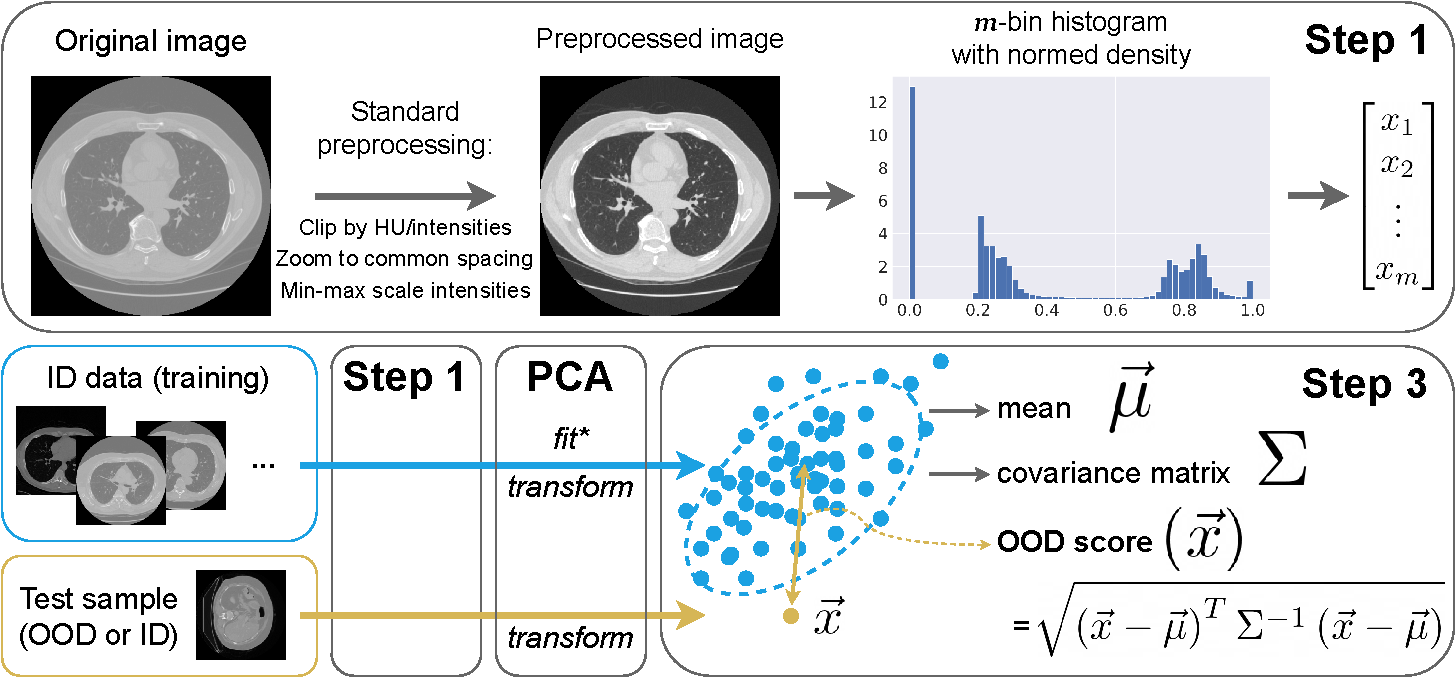
\includegraphics[width=\linewidth]{Dissertation/Figures/5_ood_bench/method-1.pdf}
	\caption{The proposed OOD detection method, called \textit{Intensity Histogram Features (IHF)}.}
	\label{fig:ihf}
\end{figure}
\end{landscape}


\section{Experiments}

\subsection{Experimental Setup}

We have 3D CT and MRI datasets with a segmentation task. So, we adhere to the standard approaches to train a segmentation model in all methods that require the latter.

\textbf{Data preprocessing.} We describe preprocessing in IHF, Step 1; it is the same in all experiments, and it is the minimum allowing the correct DL model training

\textbf{Architecture and training.} In all experiments, we use 3D U-Net \cite{isensee2018no}, a standard architecture for segmentation. We train it on patches of $64$ axial slices, with a batch size of $3$, Adam optimizer, and a learning rate of $10^{-4}$ for $30$ epochs, $1000$ iterations each. We minimize the sum of Binary Cross-Entropy and Focal Tversky losses \cite{abraham2019novel} to achieve high segmentation sensitivity. % In a batch, patches from different images are padded if necessary.

\textbf{OOD detection evaluation.} Given the ID test data, we measure the OOD detection quality against it for all the suggested OOD setups, similarly to the classification task. Outliers occur rarely in practice, so we aim to measure detection quality when most ID samples are being preserved w.r.t. relatively rare OOD events. In this case, one of the most convenient classification metrics is the false-positive rate at a 95\% true-positive rate (FPR), so we report FPR as our primary metric in Table~\ref{tab:res_fpr}. We also show AUROC in Table~\ref{tab:res_auroc} for consistency with other studies.

%\textbf{Segmentation evaluation.} We train all models on the training part of ID datasets. Then, we can evaluate their segmentation quality on the corresponding testing part of the OOD datasets, showing its possible decline. These segmentation results are given in Table~\ref{tab:segm_ct} for the CT and Table~\ref{tab:segm_mri} for the MRI datasets.


\subsection{Results}

%In this section, we start by benchmarking all considered methods, then present the analysis of the benchmark design, and conclude with the ablation study on synthetic data.

Table~\ref{tab:res_fpr} presents the primary results of our study. Uncertainty-based methods, not designed for segmentation, mostly failed in the suggested setups. Entropy, Ensemble, MCD, and G-ODIN gave substantially higher FPR than the other methods, with only G-ODIN slightly surpassing a simple \textit{Volume} predictor. Methods dedicated to segmentation performed better on average. For instance, MOOD-1 achieved 0.36 and 0.41 average FPR on CT and MRI data, respectively. SVD improved further; it appeared to be the only reliable studied method, providing 0.42 and 0.21 mean FPR.



\begin{table}[h]
	\centering
	\caption{Comparison of the considered OOD detection methods in terms of FPR@TPR95\% scores (lower is better). We highlight the best scores in every row in \textbf{bold} and ranked the methods by their average performance. The first and second sections correspond to CT and MRI setups, respectively.}
	\resizebox{\textwidth}{!}{%
		\begin{tabular}{llllllllll}
			\toprule
			\textbf{OOD Setup} &            \textbf{IHF-NN} &             \textbf{SVD} &             \textbf{IHF-Mah} &      \textbf{MOOD-1} &           \textbf{G-ODIN} &             \textbf{Volume} &   \textbf{MCD} & \textbf{Ensemble} &   \textbf{Entropy} \\
			\midrule
			Location (Head)           &  \textbf{0.00}  &  \textbf{0.00}  &  \textbf{0.00}  &            0.12 &            0.55 &            0.53 &  0.36 &     0.51 &  0.56 \\
			Location (Liver)          &            0.51 &  \textbf{0.13}  &            0.64 &            0.56 &            0.56 &            0.84 &  0.89 &     0.93 &  0.78 \\
			Population (COVID-19)     &            0.54 &            0.75 &            0.72 &  \textbf{0.51}  &            0.54 &            0.82 &  0.58 &     0.58 &  0.87 \\
			Scanner                 &            0.88 &            0.89 &            0.85 &  \textbf{0.73}  &            0.92 &            0.86 &  0.89 &     0.90 &  0.83 \\
			Synthetic (Elastic)       &  \textbf{0.15}  &            0.37 &            0.67 &            0.16 &            0.59 &            0.81 &  0.42 &     0.37 &  0.84 \\
			Synthetic (Image noise)  &            0.49 &            0.37 &            0.62 &  \textbf{0.11}  &            0.89 &            0.85 &  0.87 &     0.82 &  0.81 \\
			\midrule
			Population (Glioblastoma) &  \textbf{0.00}  &  \textbf{0.00}  &  \textbf{0.00}  &            0.10 &            0.21 &            0.01 &  0.85 &     0.81 &  0.86 \\
			Population (Healthy)      &  \textbf{0.00}  &  \textbf{0.00}  &  \textbf{0.00}  &            0.11 &  \textbf{0.00}  &  \textbf{0.00}  &  0.88 &     10.0 &  0.85 \\
			Scanner                   &  \textbf{0.00}  &  \textbf{0.00}  &  \textbf{0.00}  &            0.15 &  \textbf{0.00}  &            0.74 &  0.63 &     0.66 &  0.89 \\
			Synthetic (K-space noise) &  \textbf{0.00}  &            0.36 &  \textbf{0.00}  &            0.88 &            0.88 &            0.90 &  0.82 &     0.77 &  0.73 \\
			Synthetic (Anisotropy)    &            0.09 &            0.20 &  \textbf{0.05}  &            0.57 &            0.88 &            0.93 &  0.77 &     0.77 &  0.81 \\
			Synthetic (Motion)        &  \textbf{0.00}  &            0.58 &  \textbf{0.00}  &            0.73 &            0.93 &            0.94 &  0.85 &     0.88 &  0.91 \\
			Synthetic (Image noise)   &            0.47 &            0.33 &            0.47 &  \textbf{0.30}  &            0.56 &            0.71 &  0.78 &     0.75 &  0.75 \\
			\midrule
			CT average                &            0.43 &            0.42 &            0.58 &  \textbf{0.36}  &            0.67 &            0.79 &  0.67 &     0.68 &  0.78 \\
			MRI average               &            0.08 &            0.21 &  \textbf{0.07}  &            0.41 &            0.50 &            0.60 &  0.80 &     0.81 &  0.83 \\
			\bottomrule
	\end{tabular}}
	\label{tab:res_fpr}
\end{table}


Then, we contested SVD performance by the proposed IHF. In combination with min-distance, IHF-NN provided the best average score across studied challenges: 0.43 and 0.08 FPR, respectively. In combination with Mahalanobis distance, IHF-Mah provided practically worse results in the CT setups. Although IHF-Mah is not the best version, it was historically the first, and we submitted it to MOOD 2022 ($m=150$, no PCA). We placed second as team AIRI (\url{http://medicalood.dkfz.de/web/}, visited on 09/13/23) with the earliest IHF version, supporting its robustness by the independent evaluation.

We also conducted an ablation study to verify IHF robustness. As shown in Figure~\ref{fig:ihf_hyp}, we tested IHF performance by varying its two parameters, the number of bins ($m$) and explained variance ratio ($v$). Our findings indicated a consistent behavior regardless of the parameter choice, with a slight trend of improved quality at a larger $m$.

\begin{figure}[h]
	\centering
	% 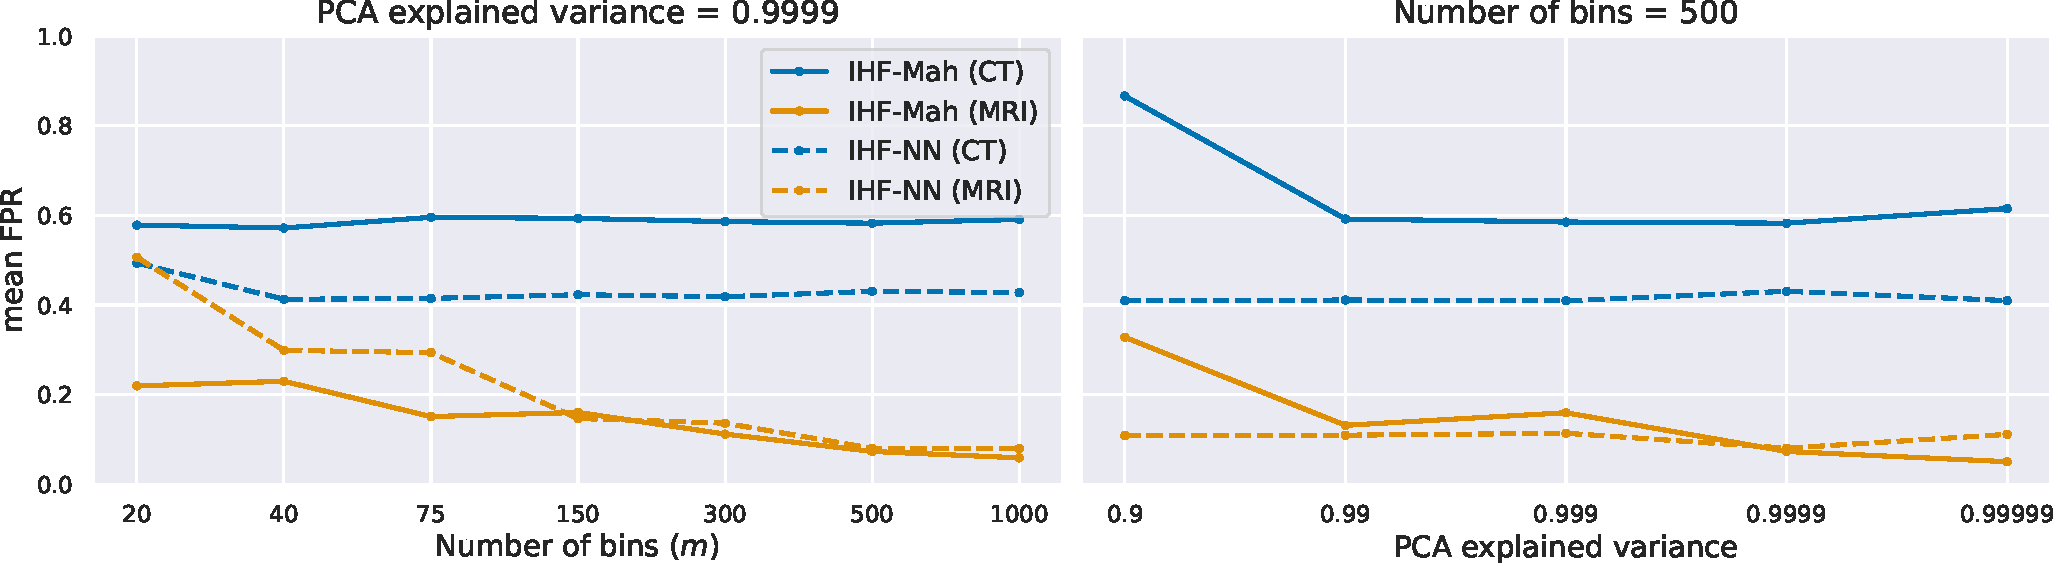
\includegraphics[width=\linewidth]{Dissertation/Figures/5_ood_bench/ihf_hyp.pdf}
	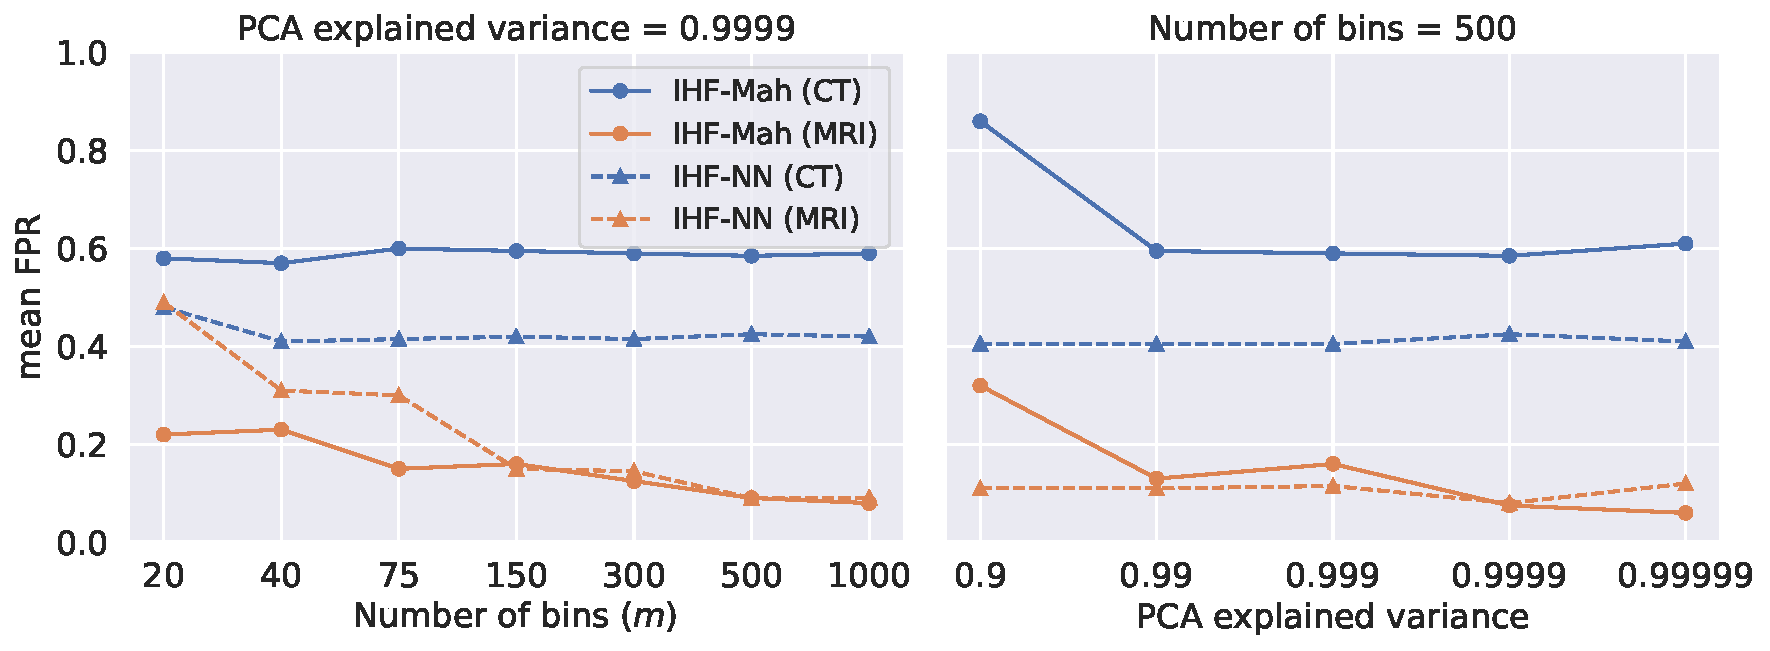
\includegraphics[width=\linewidth]{Dissertation/Figures/5_ood_bench/ihf_hyp_gost.pdf}
	\caption{Dependence of IHF on its two hyperparameters: the number of histogram bins ($m$) and explained variance in PCA ($v$).}% We give the results for both IHF variants and CT and MRI setups.}
\label{fig:ihf_hyp}
\end{figure}

Both IHF variants performed comparably or better on average than SVD and, consequently, the other studied methods. Therefore, we conclude that the histograms of image intensities are descriptive enough to detect most of the suggested OOD cases. At the same time, neural networks might omit important domain features in this problem. We thus hypothesize that neural networks-based OOD detection can be further improved and leave this promising direction for future research.

We present the same comparison in terms of AUROC in Table~\ref{tab:res_auroc}. Although AUROC is not our primary metric, it roughly preserves the same relative ranking of the studied methods, not contradicting our main message.



\begin{table}[h]
	\centering
	\caption{Comparison of OOD detection methods in terms of AUROC scores (higher is better). We highlight the best scores in every row in \textbf{bold} and ranked the methods by their average performance. The first and second sections correspond to CT and MRI setups, respectively.}
	\resizebox{\textwidth}{!}{%
		\begin{tabular}{llllllllll}
			\toprule
			\textbf{OOD Setup} &            \textbf{IHF-NN} &             \textbf{IHF-Mah} &             \textbf{SVD} &           \textbf{G-ODIN} &   \textbf{Volume} & \textbf{MOOD-1} &   \textbf{MCD} & \textbf{Ensemble} &   \textbf{Entropy} \\
			\midrule
			Location (Head)           &  \textbf{1.0}  &  \textbf{1.0}  &  \textbf{1.0}  &            0.83 &  0.73 &       0.83 &  0.85 &     0.79 &  0.62 \\
			Location (Liver)          &            0.89 &            0.85 &  \textbf{0.97}  &            0.88 &  0.65 &       0.61 &  0.42 &     0.45 &  0.67 \\
			Population (COVID-19)     &  \textbf{0.88}  &            0.83 &            0.74 &            0.86 &  0.76 &       0.66 &  0.79 &     0.80 &  0.72 \\
			Scanner                 &  \textbf{0.73}  &  \textbf{0.73}  &            0.58 &            0.72 &  0.68 &       0.51 &  0.58 &     0.55 &  0.65 \\
			Synthetic (Elastic)       &  \textbf{0.97}  &            0.83 &            0.86 &            0.85 &  0.77 &       0.78 &  0.84 &     0.85 &  0.65 \\
			Synthetic (Image noise)  &            0.81 &            0.77 &  \textbf{0.84}  &            0.75 &  0.67 &       0.80 &  0.56 &     0.61 &  0.59 \\
			\midrule
			Population (Glioblastoma) &  \textbf{1.0}  &  \textbf{1.0}  &  \textbf{1.0}  &            0.96 &  0.68 &       0.87 &  0.44 &     0.41 &  0.14 \\
			Population (Healthy)      &  \textbf{1.0}  &  \textbf{1.0}  &  \textbf{1.0}  &  \textbf{1.0}  &  0.68 &       0.86 &  0.44 &     0.16 &  0.15 \\
			Scanner                   &  \textbf{1.0}  &  \textbf{1.0}  &  \textbf{1.0}  &  \textbf{1.0}  &  0.77 &       0.83 &  0.70 &     0.74 &  0.59 \\
			Synthetic (K-space noise) &  \textbf{1.0}  &  \textbf{1.0}  &            0.86 &            0.81 &  0.66 &       0.24 &  0.56 &     0.63 &  0.66 \\
			Synthetic (Anisotropy)    &  \textbf{0.98}  &  \textbf{0.98}  &            0.94 &            0.81 &  0.68 &       0.57 &  0.63 &     0.63 &  0.71 \\
			Synthetic (Motion)        &           0.99 &  \textbf{1.0}  &            0.75 &            0.78 &  0.68 &       0.48 &  0.57 &     0.54 &  0.57 \\
			Synthetic (Image noise)   &            0.81 &            0.83 &            0.85 &  \textbf{0.88}  &  0.66 &       0.77 &  0.58 &     0.58 &  0.56 \\
			\midrule
			CT average                &  \textbf{0.88}  &            0.84 &            0.83 &            0.82 &  0.71 &       0.70 &  0.67 &     0.68 &  0.65 \\
			MRI average               &  \textbf{0.97}  &  \textbf{0.97}  &            0.92 &            0.89 &  0.69 &       0.66 &  0.56 &     0.53 &  0.48 \\
			\bottomrule
		\end{tabular}  
		
	}
	\label{tab:res_auroc}
\end{table}



\subsection{In-Depth Benchmark Analysis}

Further, we emphasize the significance of constructing a \textit{correct} benchmark to study the methods. Analysis of our experimental results suggests the following:

\begin{itemize}	
	\item OOD methods should be studied under a benchmark with diverse OOD challenges
	\item Setups should represent clinically occurring cases
	\item Potential biases in the benchmark should be explored using simple methods, such as IHF or Volume predictor
\end{itemize}

It is often possible to develop a method tailored to specific OOD sources where it thrives but fails in the other setups. For example, G-ODIN demonstrated near-perfect results in the Population and Scanner setups on MRI data but yielded the worst scores in the others. In practice, however, the precise anomaly source is always unknown, and a general OOD detector with an acceptable average performance is needed. The true method effectiveness can be estimated only in the context of diverse setups.

Secondly, OOD sources should accurately represent or simulate the clinically occurring cases. For instance, the Synthetic (Noise) setup, as introduced in \cite{zimmerer2022mood} and reproduced in our study, is not supported by any medical imaging process. MOOD-1 achieved the highest performance in this setup because its training objective is closely aligned with the anomaly synthesis process. However, performing well in this and similar cases is of no clinical value and, consequently, biases the methods' evaluation towards explicitly unrealistic scenarios.

Finally, our analysis revealed that OOD challenges might contain implicit but trivial features. If a benchmark focuses solely on any such feature, we can design a method that exploits this feature, leading to deceptive conclusions about the generalized performance. Instead, we suggest using simple methods to reveal biased features beforehand. For example, near-perfect IHF results in several setups demonstrated that certain anomalies are actually trivial intensity changes, reinforcing the need to design diverse benchmarks.

To ensure the methods' generalization, we calculate the Fechner correlation between their results and the results of the \textit{simple methods}. We show that, apart from SVD, the others exhibit a weak correlation with the Volume or IHF scores (Table~\ref{tab:res_corr}). So, the examined methods mostly do not rely on trivial features, such as image intensity distribution. However, SVD showed a correlation of 0.54 with the Volume scores, suggesting its hindered generalization on new data sources with a small difference in the predicted area volume.




\begin{table}[ht]
	\centering
	\caption{Fechner correlation coefficients between IHF-NN, Volume and the other studied methods' performance.}
	%\resizebox{\textwidth}{!}{%
		\begin{tabular}{lccccccccc}
			\toprule
			% Base method
			&  IHF-NN & SVD & IHF-M & MOOD & Godin & Vol & MCD & Ens & Ent \\
			\midrule
			IHF-NN           &  1.00 & 0.38 & \textbf{0.85} & 0.23 & -0.08 & 0.23 & 0.08 & -0.08 & -0.23 \\
			Volume          &   0.23 & \textbf{0.54} & 0.38 & 0.38 & 0.38 & 1.00 & 0.23 & 0.08 & 0.23  \\
			\bottomrule
	\end{tabular}%}
	\label{tab:res_corr}
\end{table}



\subsection{Ablation Study on Synthetic Data}

We show the OOD detection results on synthetic data for different distortion levels in Figure~\ref{fig:fpr_sev}. Distortion levels were chosen perceptually from 1 (barely noticeable distortion) to 5 (heavily distorted image). The general trend is that more distorted images are easier to detect. Here, SVD exhibited the steepest average slope and behaved almost linearly with the increasing severity level, suggesting that we have considered challenging but solvable tasks. Different methods exhibited different sensitivity to the level of distortion required for detection. Entropy and the other UE methods started to operate effectively only at level 3, while IHF detected anomalies at a minimal level. So, we conclude that the methods should be studied across a wide range of anomaly severity levels. Additionally, we show that MOOD-1 depends more on the OOD source than the severity level: it failed in Motion and K-space setups while almost perfectly detecting Noise and Elastic deformations independently of the severity level. Moreover, MOOD-1 and IHF behaved inversely to each other in Noise and Elastic setups. Such diverse behavior suggests the need to study methods across a wide range of anomaly types.

\begin{landscape}
\begin{figure}[p]
	\centering
	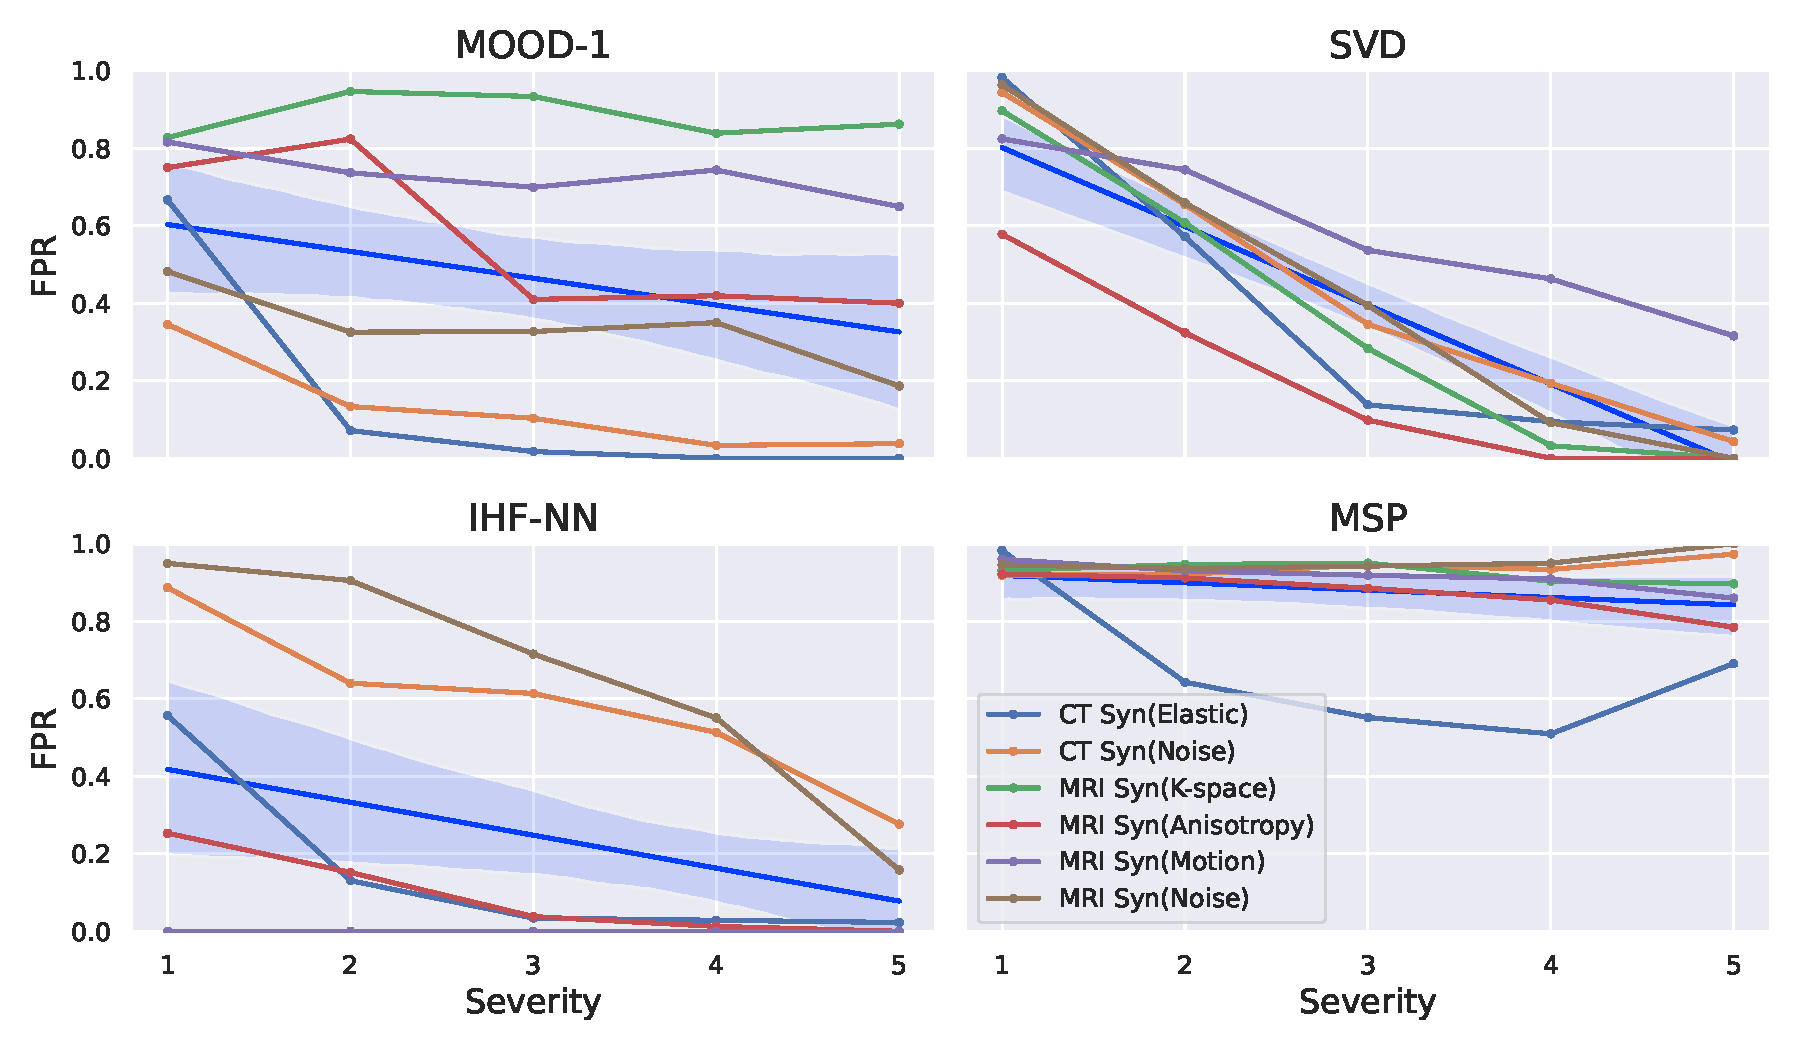
\includegraphics[width=\linewidth]{Dissertation/Figures/5_ood_bench/fpr_sev.pdf}
	\caption{FPR under synthetically distorted data for every distortion severity level. Blue line indicates method's average trend across presented challenges with 95\% confidence interval. The other UE methods (MCD, Ensemble, and G-ODIN) are excluded since their average trend is similar to Entropy.}
	\label{fig:fpr_sev}
\end{figure}
\end{landscape}



\section{Summary}

In this chapter, we have conducted an extensive investigation of OOD detection on 3D medical images. Our results revealed that the established approaches, including uncertainty estimation and anomaly detection, do not provide reliable performance. These methods predicted an unacceptably high number of false positives (0.31 mean FPR at best) and failed to generalize. We also showed that they possess a space for improvement. To do so, we developed a histogram-based method, IHF, that achieved comparable and often superior results to its competitors. Thereby, we indicated that the distribution shifts in 3D medical imaging can often be detected using intensity histograms, while the DL algorithms neglect this domain feature. Although IHF achieved better average results, its performance was surpassed in multiple challenges, emphasizing the need and possibility for developing a robust and general OOD detection method. We constructed and released the corresponding challenges as a benchmark for OOD detection on 3D medical images.%, proposing IHF as a solid baseline to contest new methods.






	\addcontentsline{toc}{chapter}{Conclusion}
\chapter*{Conclusion}


%1. Restate the Research Problem and Objectives
%Begin by briefly restating the research problem and the primary objectives of your thesis. This reminds readers of the central focus of your work.

% Example:
% "In this thesis, we addressed the challenge of integrating renewable energy sources into power systems, with a focus on improving reliability and optimizing power flow under uncertainty. Our primary objectives were to develop advanced methods for reliability assessment and to propose novel optimization techniques for chance-constrained optimal power flow."

% 2. Summarize Key Findings
% Summarize the key findings and contributions of your research. Highlight the most important results and how they address the research problem.

% Example:
% "Our research led to the development of an adaptive importance sampling method, which significantly improves the accuracy and efficiency of risk estimation for reliability constraints. Additionally, the proposed A-priori Reduced Scenario Approximation (AR-SA) method reduces the number of samples required for reliable solutions in joint chance-constrained dynamic optimal power flow problems. These methods were validated through extensive simulations, demonstrating their effectiveness in handling uncertainties in power systems."

% 3. Discuss the Significance and Impact
% Discuss the broader significance and impact of your findings. Explain how your research contributes to the field and its potential real-world applications.

% Example:
% "The findings of this thesis have significant implications for the integration of renewable energy sources into power systems. By enhancing the reliability and efficiency of power system operations, our methods support the transition to sustainable energy solutions, contributing to global efforts to reduce greenhouse gas emissions and improve energy security. Furthermore, the proposed techniques can be applied to other areas of power systems engineering, offering a foundation for future advancements in the field."

% 4. Address Limitations
% Acknowledge any limitations of your research. Being transparent about the constraints and challenges you encountered adds credibility to your work.

% Example:
% "While our methods offer substantial improvements, there are limitations to consider. The adaptive importance sampling method relies on accurate physical information, which may not always be readily available. Additionally, the computational complexity of the AR-SA method, though reduced, may still pose challenges for extremely large-scale power systems."

% 5. Suggest Future Work
% Suggest directions for future research based on your findings. Identify areas that require further investigation and how they can build on your work.

% Example:
% "Future research could explore the application of the adaptive importance sampling method to real-time power system operations, addressing the challenge of obtaining real-time physical data. Further development of the AR-SA method could focus on enhancing its scalability and applicability to even larger power grids. Additionally, integrating these methods with emerging technologies, such as smart grid systems and advanced forecasting techniques, presents a promising avenue for future work."


% 6. Final Thoughts
% Conclude with a few final thoughts that encapsulate the essence of your research and its potential to inspire further advancements in the field.

% Example:
% "In conclusion, this thesis contributes to the ongoing efforts to integrate renewable energy sources into power systems more effectively. The developed methods not only address current challenges but also pave the way for future innovations. As the global energy landscape continues to evolve, the insights gained from this research will be instrumental in shaping a sustainable and resilient energy future."


%In this thesis, we have explored various challenges and developed several methods in domain adaptation (DA) and out-of-distribution (OOD) detection within the context of 3D medical image segmentation. Throughout the chapters, a consistent theme emerges: the critical need to address distribution shifts to improve the reliability and robustness of medical image segmentation models.
%
%Starting with the analysis in Chapter~\ref{chap:mri}, we identified that low-level feature maps are particularly susceptible to domain shifts, leading to significant performance degradation. To mitigate this, we proposed fine-tuning the initial layers of the network, which proved more effective than fine-tuning the entire model, particularly in data-limited scenarios. The development of SpotTUnet further advanced this approach by autonomously determining the most affected layers, enhancing the adaptability of segmentation models across diverse medical imaging tasks.
%
%In Chapter~\ref{chap:ct}, we addressed domain shifts in CT images caused by different reconstruction kernels. We introduced FBPAug, a knowledge-driven augmentation method that improves the consistency of predictions across domains. Additionally, we developed F-Consistency, an unsupervised DA method that leverages paired CT images to achieve superior performance, particularly in challenging COVID-19 segmentation tasks. These methods collectively contribute to creating more robust segmentation models that can generalize better to unseen CT images.
%
%The M3DA benchmark introduced in Chapter~\ref{chap:da_bench} underscored the need for robust domain adaptation in medical imaging. By providing a comprehensive benchmark that covers a wide array of domain shift scenarios, we highlighted the limitations of current unsupervised DA methods, which often struggle to generalize beyond a single setup. The alternative problem settings proposed within M3DA pave the way for future research, encouraging the development of more versatile and resilient segmentation techniques. Complementing this, the BGP dataset offers a clinically realistic domain adaptation scenario with high inter-site variability, bridging the gap between methodological advances and deployment in real-world heterogeneous medical data.
%
%Finally, in Chapter~\ref{chap:ood_bench}, our investigation into OOD detection also revealed the shortcomings of existing approaches, which frequently resulted in high false-positive detection rates and thus poor model's generalization. We developed a simple (histogram-based) yet state-of-the-art (two second places in Medical Out Of Distribution Challenge 2022 and 2023 and superior performance in our proposed benchmark) method, called IHF. It could serve as a valuable tool in detecting distribution shifts that deep learning algorithms typically overlook.
%
%In conclusion, this thesis has contributed valuable insights and tools for detecting and addressing domain shifts in 3D medical image segmentation, setting the stage for further advancements in creating reliable, adaptable, and safe medical image segmentation algorithms.

This dissertation is devoted to the development of mathematically grounded and practically robust deep learning methods for domain adaptation and out-of-distribution detection in 3D medical image segmentation. The work systematically addresses the challenge of domain shift, which remains a critical obstacle to the reliable deployment of machine learning systems in clinical environments.

\begin{enumerate}
	
	\item A gradient-based supervised domain adaptation method, SpotTUnet, was proposed to address the problem of layer-wise adaptation in convolutional neural networks for medical image segmentation. The method optimizes a learnable layer selection policy, allowing to fine-tune the most shift-sensitive layers. The effectiveness of this approach was confirmed through extensive experimental validation, including statistically significant improvements over common fine-tuning baselines in few-shot adaptation scenarios. From a practical standpoint, SpotTUnet provides interpretable visualizations of domain shift sensitivity across network layers, which we further used to guide the design of F-Consistency and to enhance performance of existing DA algorithms, such as DANN~\cite{dann}, on the M3DA benchmark. Moreover, conclusions drawn from SpotTUnet contributed to the development of the IHF method for out-of-distribution detection.
	
	\item Two complementary DA methods were proposed to address performance degradation in CT segmentation caused by variations in reconstruction kernels. First, a knowledge-driven augmentation technique, Filtered Back-Projection Augmentation (FBPAug), was developed to simulate such kernel-induced domain shifts by modeling the mathematics of CT image formation in sinogram space. Second, a data-driven unsupervised DA method, F-Consistency, was introduced to align internal network representations of paired CT images reconstructed with different kernels. Both methods demonstrated statistically significant improvements over state-of-the-art approaches: FBPAug achieved high consistency in the zero-shot adaptation setting, while F-Consistency further increased segmentation quality in the standard unsupervised DA setting. FBPAug has been integrated into the production pipeline of a medical imaging startup, where it significantly improved the robustness and accuracy of CT-based segmentation models used in clinical practice.
	
	\item A large-scale benchmark, M3DA, was developed to evaluate unsupervised DA methods in 3D medical image segmentation under realistic and diverse shift scenarios. The benchmark reveals that existing methods close only 62\% of the performance gap on average. To support clinical relevance, a new multi-modal dataset, BGP, was published for glioblastoma segmentation with high intra-institution variability. These contributions enable systematic comparison of methods and guide the design of robust and generalizable DA algorithms.
	
	\item A benchmark for OOD detection in 3D medical segmentation was constructed, including clinically relevant scenarios, and was used to identify fundamental limitations of current methods. A lightweight method, IHF, was proposed as an interpretable and computationally efficient baseline, achieving top-2 in the MOOD 2022 and 2023 challenges. The benchmark and IHF serve as a foundation for further theoretical study of distributional uncertainty in medical imaging data.
	
\end{enumerate}

The results and insights of this dissertation have already served as a foundation for several subsequent scientific works. Firstly, we used the proposed OOD benchmark to develop a novel OOD detection metric and theoretically justified framework~\cite{vasiliuk2023redesigning}. We also used components of this benchmark to analyze predictive uncertainty at the level of distinct predicted components~\cite{vasiliuk2022exploring}. Finally, several colleagues’ papers~\cite{goncharov2023vox2vec,goncharov2024anatomical,goncharov2025screener} have already complemented our research by integrating FBPAug into a self-supervised learning (SSL) framework, realizing a direction for augmentation that was originally suggested in this dissertation. These works demonstrate the relevance of the presented contributions and point toward continued progress in the robust deployment of deep learning in medical imaging.

While the dissertation advances the state of domain adaptation and out-of-distribution detection in 3D medical image segmentation, several limitations define promising directions for future research.

First, SpotTUnet currently operates in a supervised DA setup and relies on annotated target samples to optimize its layer-wise adaptation policy. Extending this method to an unsupervised setting -- by introducing auxiliary domain shift criteria, e.g., domain adversarial loss function, -- could substantially increase its applicability in other experimental settings. Furthermore, as transformer-based architectures~\cite{unetr} increasingly replace convolutional backbones in segmentation models, developing analogous interpretable adaptation strategies for these architectures becomes an important task.

Second, although FBPAug and F-Consistency address the CT reconstruction kernel domain shift from complementary theoretical perspectives, they remain independent methods. A natural next step is to integrate FBPAug-generated synthetic pairs within the F-Consistency framework, thereby combining knowledge-driven and data-driven adaptation strategies into a unified self-supervised learning (SSL) approach, that may result in the inherently robust CT segmentation model. The follow-up work has already included FBPAug as an essential augmentation method into their contrastive SSL pretraining frameworks~\cite{goncharov2023vox2vec,goncharov2024anatomical}.

% the M3DA benchmark and BGP dataset currently focus on conventional convolutional DA methods. 
Third, future research should systematically evaluate emerging SSL and diffusion-based models within the M3DA and BGP benchmarks, as well as develop SSL paradigms explicitly aware of domain shifts in loss formulation. In particular, DA-aware contrastive objectives may provide a principled way to learn domain-invariant yet semantically consistent representations.

Fourth, future work in the field of OOD detection could extend the developed state-of-the-art IHF algorithm from image-level to a pixel-level one, resulting in a segmentation-level detection of anomalies. Recent progress in SSL-based anomaly localization~\cite{goncharov2025screener} highlights the feasibility of this direction, suggesting that combining pixel-wise uncertainty estimation with feature-space distribution modeling could substantially improve model interpretability and safety in clinical use. 

Overall, the presented research constitutes a systematic investigation into the reliability and robustness of deep learning models for 3D medical image segmentation under domain shift. By introducing theoretically grounded methods, publicly available benchmarks, and practically validated algorithms, this dissertation bridges the gap between academic methodology and clinical application. The results contribute to the broader effort of building \textit{trusted machine learning} in medicine -- systems that not only achieve high accuracy but also remain consistent, interpretable, and safe under real-world variability. These foundations pave the way toward the next generation of adaptive and self-aware medical artificial intelligence systems.


\section*{Acknowledgments}
The dissertation was completed at the {\thesisOrganizationEnNonTitle}.

I would like to thank everyone who has supported me throughout my academic journey and during the preparation of this thesis.

First and foremost, I am deeply thankful to my primary supervisor, Mikhail Belyaev, for his unwavering support and guidance during my Bachelor's, Master's, and Ph.D. studies. His insights into the research world and the knowledge he has shared have been invaluable in my academic and personal growth. Much of my scientific success is the result of our close collaboration and the work with his research team.

I am also deeply thankful to my collaborators and co-authors, who have greatly contributed to my scientific journey (in alphabetical order): Alexandra Dalechina, Daria Frolova, Mikhail Goncharov, Egor Krivov, Anvar Kurmukov, Ivan Oseledets, Maxim Panov, Mikhail Pautov, Maxim Pisov, Talgat Saparov, Alexey Shevtsov, Anton Vasiliuk, and Ivan Zakazov. I am fortunate to have had the opportunity to work with and learn from such brilliant people.

I am deeply thankful to my family for their constant help and belief in me.


% \newpage
% % \addcontentsline{toc}{chapter}{List of figures}
% \listoffigures

% % \addcontentsline{toc}{chapter}{List of tables}
% \listoftables
	
	\ifnumequal{\value{contnumfig}}{1}{\counterwithout{figure}{chapter}
	}{\counterwithin{figure}{chapter}}
	\ifnumequal{\value{contnumtab}}{1}{\counterwithout{table}{chapter}
	}{\counterwithin{table}{chapter}}
	
	
	
	% \printnomenclature[3.5cm] % Значение ширины столбца с обозначениями стоит подбирать вручную


\addcontentsline{toc}{chapter}{List of symbols and abbreviations}
\chapter*{List of symbols and abbreviations}

\begin{tabularx}{0.9\textwidth}{lX}
	AD & Anomaly Detection \\
	AUROC & Area Under Receiver Operating Characteristic (Curve) \\
	BCE & Binary Cross-Entropy \\
	BGP & Burdenko’s Glioblastoma Progression \\
	BN & Batch Normalization \\
	CE & Contrast Enhancement \\
	CNN & Convolutional Neural Network \\
	COVID-19 & Coronavirus Disease 2019 \\
	CT & Computer Tomography \\
	DA & Domain Adaptation \\
	DANN & Domain Adversarial Neural Network \\
	DL & Deep Learning \\
	DNN & Deep Neural Network \\
	DSC & Dice Similarity Coefficient \\
	FBP & Filtered Back-Projection \\
	% FDA & Fourier Domain Adaptation \\
	FPR & False-Positive Rate \\
	GAN & Generative Adversarial Network \\
	GGO & Ground-Glass Opasity \\
	GTV & Gross Tumor Volume \\
	HM & Histogram Matching \\
	HU & Hounsfield Units \\
	ID & In-Distribution \\
	IHF & Intensity Histogram Features \\
	IN & Instance Normalization \\
	LDCT & Low Dose Computer Tomography \\
	MCD & Monte-Carlo Dropout \\
	MRI & Magnetic Resonance Imaging \\
	MSE & Mean Squared Error \\
	NN & Neural Network \\
	OOD & Out-of-Distribution \\
	PCA & Principal Component Analysis \\
	ROI & Region of Interest \\
	
	
	 %%%%%%%%
	
%    $I$ & Identity matrix \\
%    $1$ & Vector of ones \\
%    $A^*$ & Complex conjugate of a matrix \\
%    $A^\top$ & Transpose of a matrix \\
%    $\|A\|_p$ & Operator $p$-norm of a linear operator, $2$-norm of a linear operator if not specified \\
%    $\mathbbm{C}$ & The field of complex numbers \\
    
%    $\mathbb{P}$ & Probability measure \\
%    $\mathbb{E}$ & Mathematical expectation \\
%    $\mathbb{V}$ & Variance \\
%    $\textup{KL}$ & Kullback-Leibler divergence \\
%    $\mathcal{N}(\mu, \Sigma)$ & Gaussian distribution with mean vector $\mu$ and covariance matrix $\Sigma$\\
%    $1\left[A\right]$ & Indicator of the event $A$ \\
%    $\rmi$ & Imaginary unit \\
%    $\nabla $ & Nabla operator \\
%    $\Phi(\cdot)$ & Cumulative Distribution Function (CDF) of the standard Gaussian distribution\\
\end{tabularx}

\begin{tabularx}{0.9\textwidth}{lX}
	SDA & Supervised Domain Adaptation \\
	% SE & Self-Ensembling \\
	SGD & Stochastic Gradient Descent \\
	SVD & Singular Value Decomposition \\
	T & Tesla, unit of magnetic flux density \\
	TPR & True-Positive Rate \\
	TL & Transfer Learning \\
	UDA & Unsupervised Domain Adaptation \\
	UE & Uncertainty Estimation \\
	$\R$ & The field of real numbers \\
	$\mathcal{F}\left[ \cdot \right]$ & Fourier transform of the input function \\
	$\kappa(t)$ & Ramp filter \\
	$\mathcal{R}\left( \cdot \right)$ & Radon transform of the input image \\
%    $I$ & Identity matrix \\
%    $1$ & Vector of ones \\
%    $A^*$ & Complex conjugate of a matrix \\
    $A^\top$ & Transpose of a matrix \\
    $\| \cdot \|_p$ & Operator $p$-norm of a tensor \\%, $2$-norm of a linear operator if not specified \\
%    $\mathbbm{C}$ & The field of complex numbers \\
%    $\mathbb{P}$ & Probability measure \\
%    $\mathbb{E}$ & Mathematical expectation \\
%    $\mathbb{V}$ & Variance \\
%    $\textup{KL}$ & Kullback-Leibler divergence \\
%    $\mathcal{N}(\mu, \Sigma)$ & Gaussian distribution with mean vector $\mu$ and covariance matrix $\Sigma$\\
%    $1\left[A\right]$ & Indicator of the event $A$ \\
%    $\rmi$ & Imaginary unit \\
%    $\nabla $ & Nabla operator \\
%    $\Phi(\cdot)$ & Cumulative Distribution Function (CDF) of the standard Gaussian distribution\\
\end{tabularx}

%\item 
%\item FBPAug -- Filtered Back-Projection Augmentation
%\item 
%\item 

%\item         % Список сокращений и условных обозначений
	% \chapter*{Словарь терминов}             % Заголовок
\addcontentsline{toc}{chapter}{Словарь терминов}  % Добавляем его в оглавление

\textbf{TeX} : Cистема компьютерной вёрстки, разработанная американским профессором информатики Дональдом Кнутом

\textbf{панграмма} : Короткий текст, использующий все или почти все буквы алфавита
      % Словарь терминов
	\clearpage                                  % В том числе гарантирует, что список литературы в оглавлении будет с правильным номером страницы
\urlstyle{rm}                               % ссылки URL обычным шрифтом
\ifdefmacro{\microtypesetup}{\microtypesetup{protrusion=false}}{} % не рекомендуется применять пакет микротипографики к автоматически генерируемому списку литературы

% Подсчёт общего числа записей
%\printbibliography[env=counter, keyword=bibliofull, section=0, heading=nobibheading]

%\insertbibliofull                           % Подключаем Bib-базы: все статьи единым списком
\insertbiblioexternal                      % Подключаем Bib-базы: статьи, не являющиеся статьями автора по теме диссертации
\insertbiblioauthor                        % Подключаем Bib-базы: работы автора единым списком 
%\insertbiblioauthorgrouped                 % Подключаем Bib-базы: работы автора сгруппированные (ВАК, WoS, Scopus и т.д.)
\insertbiblioregistered


\printbibliography[env=counter, keyword=bibliofull, heading=nobibheading]


\ifdefmacro{\microtypesetup}{\microtypesetup{protrusion=true}}{}
\urlstyle{tt}                               % возвращаем установки шрифта ссылок URL      % Список литературы
	\clearpage
\ifdefmacro{\microtypesetup}{\microtypesetup{protrusion=false}}{} % не рекомендуется применять пакет микротипографики к автоматически генерируемым спискам
\listoffigures  % Список изображений

%%% Список таблиц %%%
% (ГОСТ Р 7.0.11-2011, 5.3.10)
\clearpage
\listoftables   % Список таблиц
\ifdefmacro{\microtypesetup}{\microtypesetup{protrusion=true}}{}
\newpage           % Списки таблиц и изображений (иллюстративный материал)
	
	\setcounter{totalchapter}{\value{chapter}} % Подсчёт количества глав
	
	
	%%% Настройки для приложений
	\appendix
	% Оформление заголовков приложений ближе к ГОСТ:
	\setlength{\midchapskip}{20pt}
	\renewcommand*{\afterchapternum}{\par\nobreak\vskip \midchapskip}
	%\chapter{M3DA datasets description}
%\label{app:m3da_datasets}
%
%
%Below we provide an extended description of datasets used in M3DA benchmark, download and usage examples are available in the published repository\footnote{\href{https://github.com/BorisShirokikh/M3DA}{https://github.com/BorisShirokikh/M3DA}}. Example 2D slices from every dataset for visual comparison between domains are given in Figure~\ref{fig:contours}. Summary of licenses and data access is given in Table~\ref{tab:supp_datasets}.
%
%\begin{table}[h]
	\centering
	\caption{Datasets licenses and independent source links.}
	
	\resizebox{\linewidth}{!}{%
		\begin{tabular}{@{}lcc@{}}
			\toprule
			\textbf{Dataset} & license & link to dataset \\
			\midrule
			BraTS \cite{brats} & CC BY 4.0  & \href{https://www.cancerimagingarchive.net/analysis-result/rsna-asnr-miccai-brats-2021/}{https://www.cancerimagingarchive.net/analysis-result/rsna-asnr-miccai-brats-2021/} \\
			
			CC359 \cite{cc359} & CC BY-ND 4.0 & \href{https://www.ccdataset.com/download}{https://www.ccdataset.com/download}  \\
			
			AMOS \cite{amos} & CC BY 4.0 & \href{https://zenodo.org/records/7262581}{https://zenodo.org/records/7262581} \\
			
			AMOS LDCT & CC BY 4.0 & \href{https://zenodo.org/records/13373720}{https://zenodo.org/records/13373720} \\
			
			LIDC \cite{lidc} & CC BY 3.0 & \href{https://www.cancerimagingarchive.net/collection/lidc-idri/}{https://www.cancerimagingarchive.net/collection/lidc-idri/}\\
			
			\bottomrule
		\end{tabular}
	}
	\label{tab:supp_datasets}
\end{table}
%
%
%\section{AMOS}
%
%The AMOS dataset \cite{amos} contains 500 CT and 100 MRI abdominal scans with the multi-organ segmentation task: liver, stomach, spleen, left and right kidneys, bladder, aorta, pancreas, inferior vena cava, duodenum, prostate/uterus, gallbladder, esophagus, left and right adrenals. As a largest available dataset for inter-modality segmentation, we employed it in MR$\ra$CT and CT$\ra$MR domain shift setups. 
%
%We used all 60 labeled MRIs as the \textit{source} set in MR$\ra$CT setup and the \textit{target test} set in CT$\ra$MR. Then, 200 unlabeled CTs and 40 unlabeled MRIs were used as the \textit{target train} sets for adaptation purposes in the MR$\ra$CT and CT$\ra$MR setups, respectively. The remaining 300 labeled CTs were evenly split in two groups: the first is a source set in CT$\ra$MR, and the second is a target test set in MR$\ra$CT.
%
%Furthermore, we used AMOS CT images to create one of the most clinically relevant domain shift setups -- difference in the radiation dose during scanning. 
%% In CT$\ra$LDCT, we employed the first group of 150 labeled CTs as a source set, 200 unlabeled CTs as a target train set, and the second group of 150 labeled CTs as a target test set. 
%For the LDCT domain, we simulated low radiation dose using the algorithm provided in \cite{ldct}, simulated data are available at \href{https://zenodo.org/records/13373720}{https://zenodo.org/records/13373720}.
%
%
%\section{BraTS}
%
%BraTS \cite{brats} is comprised of 2000 brain MRI cases, each consisting of four sequences: T1, T1c, T2, FLAIR, with a glioblastoma segmentation classes (3 foreground classes and background).  We only used 1251 cases with publicly available annotations and T1, T1c MRI sequences for T1 CE$\ra$T1 shift. Since sequences of the same case provide information about the same subject, we ensured source-target splits so that every case falls into exactly one fold and split cases with 50:25:25 ratio into source, target train, and target test folds.
%
%
%\section{CC359}
%
%The CC359 dataset \cite{cc359} contains 359 brain MR T1 images from three scanners, namely, GE, Philips (PH), and Siemens (SM), obtained using two magnetic field strength values, $1.5$ and $3.0$T. The dataset can be split into six domains defined by two different field strengths $\times$ three vendors, each with approximately 60 images, so it yields 30 possible domain adaptation pairs. 
%
%CC359 also offers three tasks: brain, hippocampus, and white matter, gray matter, and cerebrospinal fluid (WMGMCSF) segmentation. We ommited hippocampus segmentation task from the benchmark, because our preliminary experiments showed it is not significantly affected by domain shifts, the relative performance drop is less than $2\%$ in every domain pair; see Table~\ref{tab:hippo}. We also omitted the brain segmentation task for the same reason, see results in \cite{shirokikh2020first}.
%
%

\begin{table}[h]
	\centering
	\caption{Baseline and oracle results on the CC359 WMGMSCF segmentation task.}
	\label{tab:wmgmcsf}
	
	% \resizebox{\columnwidth}{!}{%
		\begin{tabular}{|c|l||c|c|c|c|c|c|}
			
			\hline
			\multicolumn{2}{|l||}{\multirow{2}{*}{}}  & \multicolumn{6}{c|}{Target domains}\\ 
			\cline{3-8}
			\multicolumn{2}{|l||}{} & GE1.5 & PH1.5 & SM1.5 & GE3.0 & PH3.0 & SM3.0\\ 
			\hline
			\hline
			
			% \clrtb
			
			\multirow{6}{*}{{\rotatebox[origin=c]{90}{Source domains}}}
			& GE 1.5 & 95.8 & 82.1 & 90.8 & 82.1 & 92.6 & 80.8 \\
			\cline{2-8}
			
			& PH 1.5 & 80.1 & 92.7 & 90.8 & 93.4 & \textbf{74.1} & 90.1 \\
			\cline{2-8}
			
			& SM 1.5 & 89.7 & 85.3 & 95.6 & 86.2 & 86.2 & 84.5 \\
			\cline{2-8}
			
			& GE 3.0 & 76.6 & 89.9 & 90.3 & 95.9 & 72.0 & 91.4 \\
			\cline{2-8}
			
			& PH 3.0 & 90.6 & 74.7 & 86.0 & 75.4 & 95.4 & \textbf{76.6} \\
			\cline{2-8}
			
			& SM 3.0 & \textbf{56.0} & 88.6 & 84.9 & 92.4 & 68.4 & 95.7 \\
			\hline
			
		\end{tabular}%}
\end{table}


\begin{table}[h]
	\centering
	\caption{Baseline and oracle results on the CC359 hippocampus segmentation task.}
	\label{tab:hippo}
			
	%\resizebox{\columnwidth}{!}{%
		\begin{tabular}{|c|l||c|c|c|c|c|c|} 
			\hline
			\multicolumn{2}{|l||}{\multirow{2}{*}{}}  & \multicolumn{6}{c|}{Target domains}\\ 
			\cline{3-8}
			\multicolumn{2}{|l||}{} & GE1.5 & PH1.5 & SM1.5 & GE3.0 & PH3.0 & SM3.0 \\ 
			\hline
			\hline
			
			% \clrtb
			
			\multirow{6}{*}{{\rotatebox[origin=c]{90}{Source domains}}}
			& GE 1.5 & 92.3 & 86.7 & 88.7 & 87.8 & 91.2 & 91.2 \\
			\cline{2-8}
			
			& PH 1.5 & 91.3 & 86.9 & 87.7 & 87.7 & 89.7 & 89.9 \\
			\cline{2-8}
			
			& SM 1.5 & 91.7 & 86.6 & 89.3 & 88.2 & 90.9 & 90.8 \\
			\cline{2-8}
			
			& GE 3.0 & 91.4 & 86.4 & 88.0 & 89.1 & 90.5 & 91.3 \\
			\cline{2-8}
			
			& PH 3.0 & 91.5 & 86.5 & 88.3 & 87.7 & 92.0 & 91.0 \\
			\cline{2-8}
			
			& SM 3.0 & 90.8 & 86.5 & 87.8 & 88.0 & 90.6 & 92.1 \\
			\hline
			
	\end{tabular}%}
\end{table}

%
%Therefore, we focus only on the WMGMCSF segmentation task in CC359: white matter, gray matter and cerebral spinal fluid segmentation classes and background. From 30 possible domain pairs, we selected three with the maximum performance drop, highlighted in \textbf{bold},  Table~\ref{tab:wmgmcsf}): changing field strength with a fixed scanner PH 1.5T $\ra$ PH 3.0T (drop from 95.4 to 74.1 Dice score), changing scanner with the fixed field strength PH 3.0T $\ra$ SM 3.0T (drop from 95.7 to 76.6), and changing both parameters SM 3.0T $\ra$ GE 1.5T (drop from 95.8 to 56.0). We denote them as T1 F, T1 Sc, and T1 Mix, respectively.
%
%
%\section{LIDC}
%
%LIDC \cite{lidc} is a multi-center collection of diagnostic and lung cancer screening thoracic CT scans with annotated lesions. It includes 1308 studies (of which 1018 include CT studies) from 1010 patients. Lung's nodules is one of the few clinical applications where both CE CT and CT are used, first for the initial scan, and second for the follow-ups \cite{purysko2016does}. We used LIDC for CE CT $\ra$ CT domain shift, we split data into three roughly equal groups, ommiting scans with empty masks: contrast enhanced CT (source domain) $X^s$, CT without contrast enhancement $X^t_{tr}$ (training part, target domain), and CT without contrast enhancement  $X^t_{ts}$ (test part, target domain). $X^t_{tr}$ and $X^t_{ts}$ were stratified by the number of lesions.
%
%
%\chapter{M3DA methods description}
%\label{app:m3da_methods}
%
%As mentioned above, we used an nnU-Net \cite{nnunet} backbone as segmentation network architecture in all methods. We preserved most of the nnU-Net training pipeline except for several methodological changes, which allow us to evaluate DA methods, such as AdaBN and InstanceNorm, separately and run the ablation studies. These changes along with the other training hyper-parameters are summarized in Table~\ref{tab:hyper}.
%
%Firstly, we replaced the default InstanceNorm with BatchNorm layers and removed test-time augmentation, so we can compare different normalizations and adaptive normalizations (AdaBN) and assess the unhindered impact of DA methods. Secondly, we reduced the patch size and number of the network features, so all experiments fit in a single 16 GB NVIDIA Tesla V100 and our benchmark remains economical. We set the number of epochs to 600 in all experiments, so that any method could complete its training in three days. All experiments were conducted on the Zhores supercomputer~\cite{zacharov2019zhores}.
%
%

\begin{table}[h]
	\centering
	\caption{Hyper-parameters.}
	\label{tab:hyper}
	%\resizebox{\linewidth}{!}{
		\begin{tabular}{lcc}
			\toprule 
			\textbf{hyper-parameter} & \textbf{nnUNet} & \textbf{U-Net (ours)}  \\ 
			\midrule
			architecture & auto & auto \\
			base features & 32 & 24 \\
			normalization & instance (IN) & batch (BN) \\
			batch size & 2 & 2 \\
			patch size & (160, 192, 64) & (160, 160, 64) \\
			epochs & 600 & 600 \\
			batches per epoch & 250 & 250 \\
			loss & Dice Loss + CE & Dice Loss + CE \\
			% loss masking based on intensity & \cmark & \xmark \\
			oversampling rate & 0.66 & 0.75 \\
			optimizer & SGD & SGD \\
			momentum & 0.99 & 0.99 \\
			weight decay & $3 \times 10^{-5}$  & $3 \times 10^{-5}$ \\
			initial learning rate & $10^{-2}$ & $10^{-2}$ \\
			learning rate schedule & poly decay & poly decay \\
			learning rate decay power & 0.9 & 0.9 \\
			test-time augmentation & \cmark & \xmark \\
			\bottomrule
	\end{tabular}%}
\end{table}

%
%Below, we provide DA methods implementation details:
%
%\paragraph{Histogram matching} uses the baseline training pipeline, except all image intensity histograms are equalized to an average histogram computed over the train set. 
%
%\paragraph{Gamma augmentation} also uses the baseline training pipeline, and we perform gamma correction with randomly selected $\gamma \sim U[0.5, 2]$ on every input image.
%
%\paragraph{nnAugm} similarly supplements the same baseline training with the original set of nnUNet \cite{nnunet} augmentations.
%
%\paragraph{InstanceNorm} substitutes BN layers, while the training pipeline remains the same as in baseline.
%
%\paragraph{Adaptive BN} performs additional 1000 inference steps with batch size 4 over the baseline, updating the running statistics of BN layers on target training data.
%
%\paragraph{Self-ensembling} design and all parameters are reproduced from \cite{se_medim} with our architecture.
%
%\paragraph{MinEnt} adds a predictions entropy minimization criterion on target images. So we extended our training pipeline with the second step using target train images, and added entropy loss with the recommended in \cite{entropy} weight $\lambda = 0.001$.
%
%\paragraph{DANN} introduces an auxiliary network called discriminator. Similar to recent studies \cite{entropy}, we used DCGAN~\cite{dcgan} discriminator architecture, replacing 2D convolutions with 3D ones. The losses weighting parameter is taken from \cite{dann_medim}, e.g., $\alpha = 0.01$.
%
%\paragraph{CycleGAN 2D} is fully reused from the original study \cite{cyclegan}. We trained a standalone CycleGAN 2D to map between source and target train images, where we sample axial slices from our volumetric images and rescale them into 256 $\times$ 256 gray scale images. Before predicting with the baseline segmentation model, we applied one of the generators to target test images (slice-by-slice) to transform them into fake source ones.
%
%\paragraph{CycleGAN 3D} is fully reused from the original study \cite{cyclegan3d}. We trained a standalone CycleGAN 3D to map between source and target train images, where we sample patches of size (128, 128, 96) from our volumetric images. Before predicting with the baseline segmentation model, we applied one of the generators to target test images (via overlapping grid) to transform them into fake source ones.
%
%\paragraph{GIN} is fully reused from \cite{gin} with the implementation based on the nnU-Net framework.
%
%\paragraph{MIND} is fully reused from \cite{dg_tta} with the implementation based on the nnUNet framework.\\
%
%
%All experiments are available at \href{https://github.com/BorisShirokikh/M3DA-exp}{github.com/BorisShirokikh/M3DA-exp}.


%\chapter{Evidence of Industrial Application}
%\label{app:m3da_datasets}
\chapter{Certificate of Registration}
\label{app:reg}

\begin{center}
	%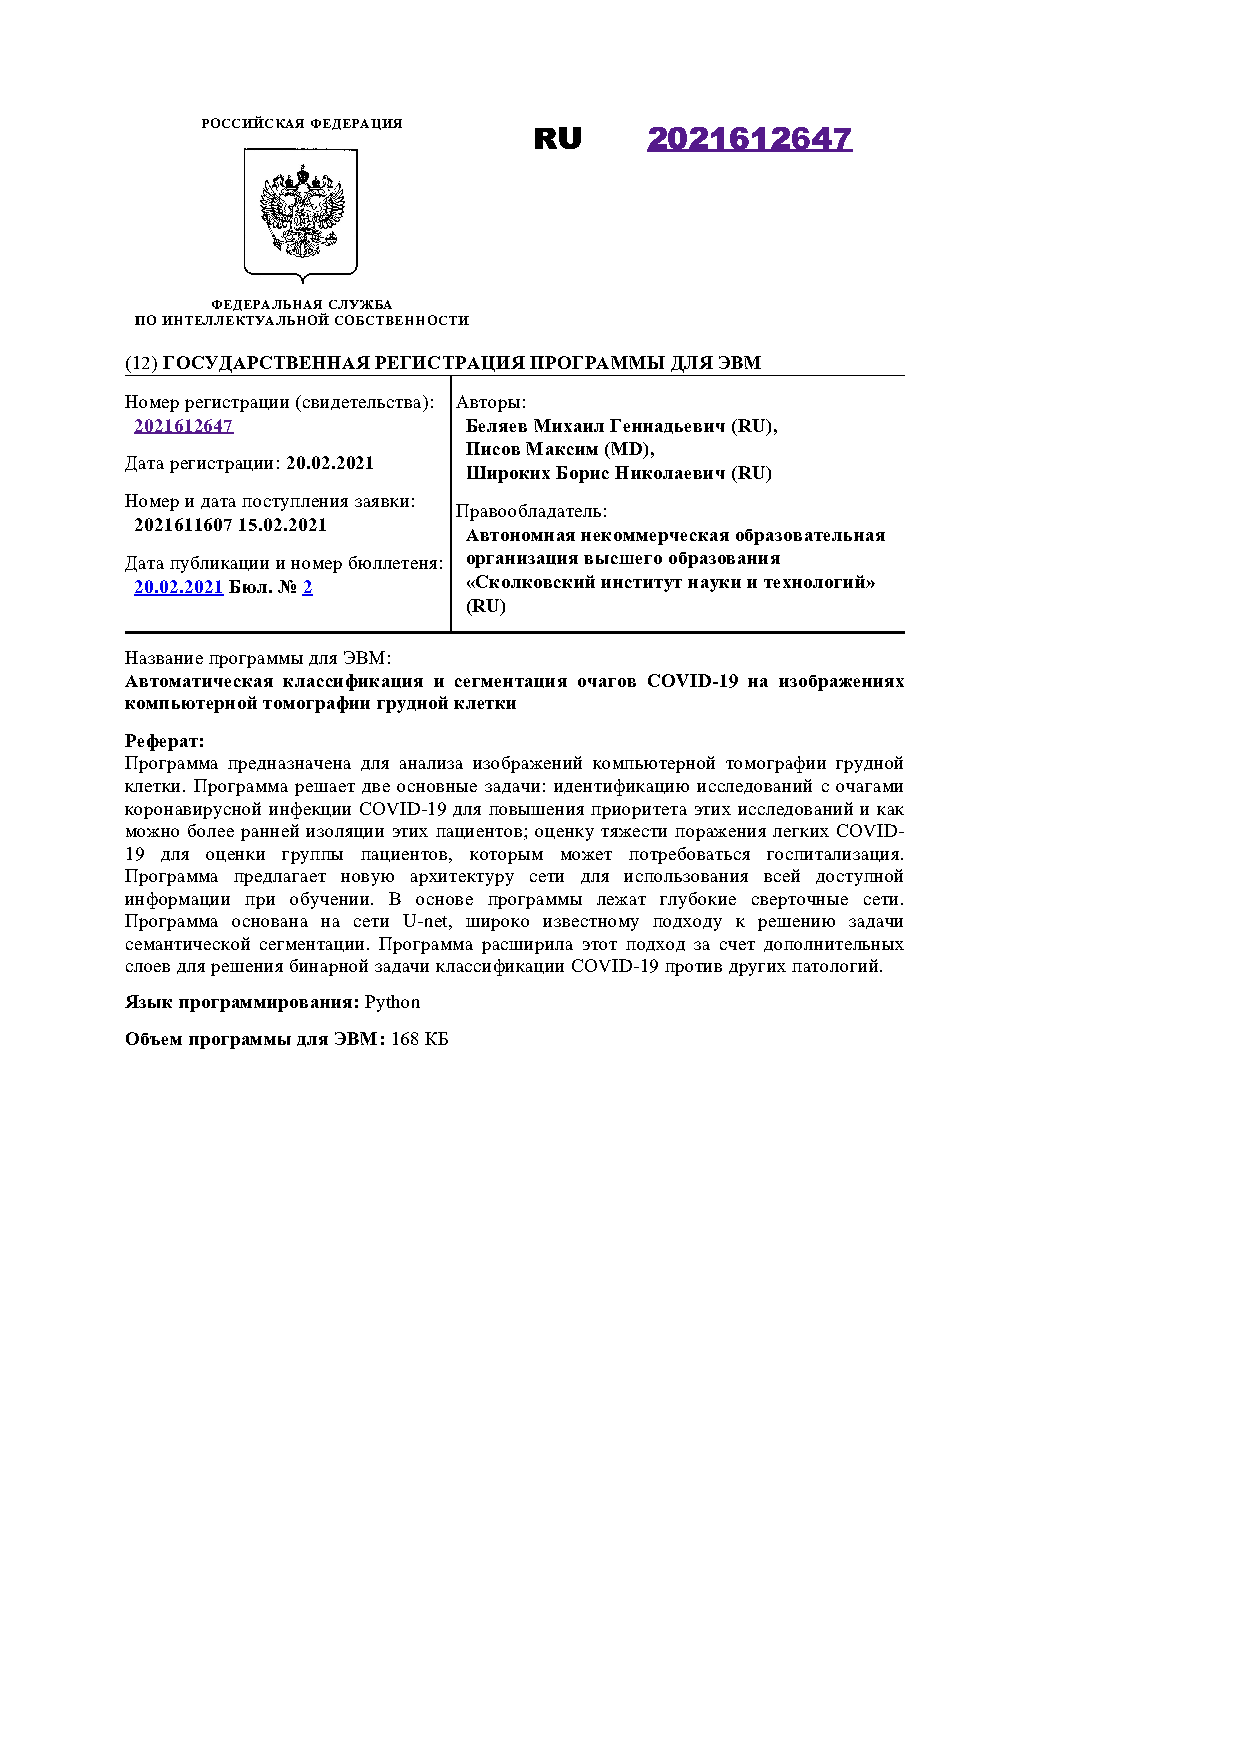
\includegraphics[width=\textwidth]{Dissertation/Figures/6_appendix/output.pdf}
	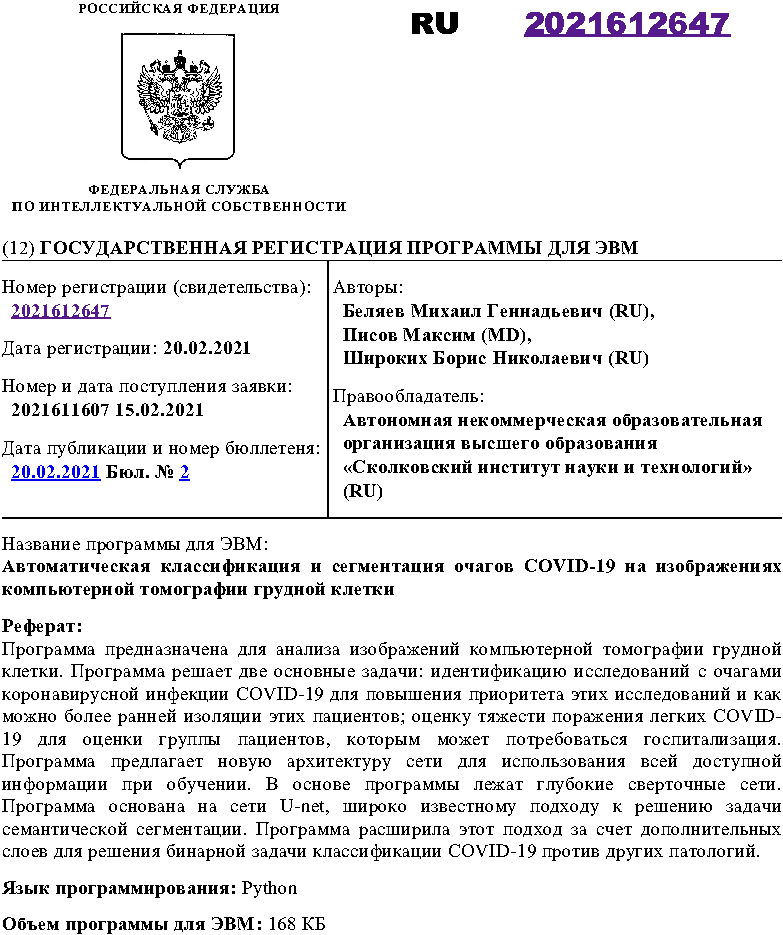
\includegraphics[width=0.95\textwidth]{Dissertation/Figures/6_appendix/output_crop.pdf}
\end{center}

        % Приложения
	
	\setcounter{totalappendix}{\value{chapter}} % Подсчёт количества приложений
	
\end{document}
